\documentclass[a4paper,11pt]{article}
\usepackage[table]{xcolor}



\newcommand{\defeq}{\mathrel{\doteq}}

\newcommand{\lzero}{0}

\newcommand{\kw}[1]{\mathtt{#1}}

\newcommand{\expr}{e}
\newcommand{\vall}{w}
\newcommand{\valr}{v}
\newcommand{\eif}{\kw{if}}
\newcommand{\eapp}{\;}
\newcommand{\eprojl}{\kw{fst}}
\newcommand{\eprojr}{\kw{snd}}
%\newcommand{\eprov}[1]{\eta_{#1}}
\newcommand{\etrue}{\kw{true}}
\newcommand{\efalse}{\kw{false}}
\newcommand{\econst}{c}
\newcommand{\eop}{\delta}
\newcommand{\efix}{\mathop{\kw{fix}}}
%\newcommand{\labelA}{\ell}

\newcommand{\tr}{T}
\newcommand{\trift}{\eif^{\kw{t}}}
\newcommand{\triff}{\eif^{\kw{f}}}
\newcommand{\trprojl}{\eprojl}
\newcommand{\trprojr}{\eprojr}
\newcommand{\trtrue}{\etrue}
\newcommand{\trfalse}{\efalse}
\newcommand{\trconst}{\econst}
\newcommand{\trop}{\eop}
\newcommand{\trfix}{\efix}
\newcommand{\trapp}[5]{#1 \; #2 \mathrel{\triangleright} {\efix #3(#4).#5}}

\newcommand{\adap}{\kw{adap}}
\newcommand{\ddep}[1]{\kw{depth}_{#1}}
\newcommand{\nat}{\mathbb{N}}
\newcommand{\natb}{\nat_{\bot}}
\newcommand{\natbi}{\natb^\infty}
\newcommand{\nnatA}{n}
\newcommand{\nnatB}{m}
\newcommand{\nnatbA}{s}
\newcommand{\nnatbB}{t}
\newcommand{\nnatbiA}{q}
\newcommand{\nnatbiB}{r}

\newcommand{\type}{\tau}
\newcommand{\tbase}{\kw{b}}
\newcommand{\tbool}{\kw{bool}}
\newcommand{\tarr}[5]{#1; #3 \xrightarrow{#4; \, #5} #2}
\newcommand{\env}{\theta}

\newcommand{\bigstep}{\mathrel{\Downarrow}}

\newcommand{\dmap}{\rho}
\newcommand{\dmapb}{\bot_\dmap}
\newcommand{\supp}{\kw{supp}}
\newcommand{\dom}{\kw{dom}}

\newcommand{\tvdash}[1]{\vdash_{#1}}

%Packages
\usepackage[T1]{fontenc}
\usepackage{fourier} 
\usepackage[english]{babel} 
\usepackage{amsmath,amsfonts} 
\usepackage{amsthm} 
\usepackage{color}   %May be necessary if you want to color links
\usepackage{hyperref}
\usepackage{lscape}
\usepackage{geometry}
\usepackage{amsmath}
\usepackage{algorithm}
\usepackage{algorithmic}
\usepackage{amssymb}
\usepackage{amsfonts}
\usepackage{times}
\usepackage{bm}
\usepackage{ stmaryrd }
\SetSymbolFont{stmry}{bold}{U}{stmry}{m}{n}

\usepackage{ amssymb }
\usepackage{ textcomp }
\usepackage[normalem]{ulem}
% For derivation rules
\usepackage{mathpartir}
\usepackage{color}
\usepackage{a4wide}
\usepackage{caption}
\usepackage{subcaption}
\usepackage{mathpartir}
\usepackage{amsmath,amsfonts}
\usepackage{ amssymb }
\usepackage{color}
\usepackage{algorithm}
\usepackage{algorithmic}
\usepackage{microtype}
\usepackage{eucal}
\usepackage{url}
\usepackage{xspace}
\usepackage{array}
\usepackage{listings}

\usepackage{tikz}
\usetikzlibrary{shapes.geometric}
\usetikzlibrary{arrows.meta,arrows}
\usetikzlibrary{decorations.text}
% % % % 


\usepackage{multirow}


%%%%%%%%%%%%%%%%%%%%%%%%%%%%%%%%%%%%%%%%%%%%%%%%%%%%%Packages And Definitions For Listing the Code%%%%%%%%%%%%%%%%%%%%%%%%%%%%%%%%%%%%%%%%%%%%%%%%%%%%%%%%%%%%%%%%%%%%%%%%
\usepackage{listings}
\usepackage{xcolor}

\definecolor{codegreen}{rgb}{0,0.6,0}
\definecolor{codegray}{rgb}{0.5,0.5,0.5}
\definecolor{codepurple}{rgb}{0.58,0,0.82}
\definecolor{backcolour}{rgb}{0.95,0.95,0.92}

\lstdefinestyle{mystyle}{
    backgroundcolor=\color{backcolour},   
    commentstyle=\color{codegreen},
    keywordstyle=\color{magenta},
    numberstyle=\tiny\color{codegray},
    stringstyle=\color{codepurple},
    basicstyle=\ttfamily\footnotesize,
    breakatwhitespace=false,         
    breaklines=true,                 
    captionpos=b,                    
    keepspaces=true,                 
    numbers=left,                    
    numbersep=5pt,                  
    showspaces=false,                
    showstringspaces=false,
    showtabs=false,                  
    tabsize=2
}

\lstset{style=mystyle}

\usepackage{tikz}
\usetikzlibrary{shapes,arrows}
\newcommand{\THESYSTEM}{\textsf{AdaptFun}}

% Define block styles
\tikzstyle{decision} = [diamond, draw, fill=blue!20, 
    text width=4.5em, text badly centered, node distance=3cm, inner sep=0pt]
\tikzstyle{block} = [rectangle, draw, fill=blue!20, 
    text width=5em, text centered, rounded corners, minimum height=4em]
\tikzstyle{line} = [draw, -latex']
\tikzstyle{cloud} = [draw, ellipse,fill=red!20, node distance=3cm,
    minimum height=2em]

\begin{document}
\title{Program Analysis for Adaptivity Analysis}

\author{}

\date{}

\maketitle


\tableofcontents


% \section{Introduction}
\section{System Overview}


\section{Labeled {\tt While} Language}
\label{sec:while_language}
%
\subsection{Syntax and Semantics}
%
\paragraph{Language}
\begin{figure}[h]
	$$
	\begin{array}{rcl}
		\text{Types} & \quad & \tau ::= b \sep \tau \multimap \tau' \sep !_n \tau \sep
		\tau \times \tau \sep \tforallN{i}{\tau} \sep \query \\[2mm]
   
		\text{Term} & \quad & t ::= c \sep \fix{t} \sep \app{t}{t} \sep !t \sep (t_1,t_2) \sep  \letx{!x}{t_1}{t_2} \sep \Lambda.t \sep t[] \sep \abs{x}{t} \sep  M(t) \sep x \sep q \sep\\
		&& \quad   \tcaseof{t}\ \{c_i \Rightarrow t_i\}_{c_i \in b}  \sep \letx{(x_1,x_2)}{t_1}{t_2} \\[2mm]
		 
		\text{Normal Form} &\quad & v ::=  c \sep \fix{t} \sep !t \sep (v_1, v_2) \sep \Lambda. t \sep \abs{x}{t}  \sep x \sep q \sep \tcaseof{v}\ \{c_i \Rightarrow v_i\}_{c_i \in b_i} \sep\\
		&& \enil \sep \econs(v_1,v_2)  \\[2mm]
   
		\text{Mechanisms} &\quad & M ::=  {\tt gauss} \sep {\tt thdt} \\[2mm]
   
   
	   \text{Tree} &\quad& T_b :: = c \sep M(T_{query}) \sep \tcaseof{T_b}\ \{ c_i \Rightarrow T_{b_i}\}_{c_i \in b} \\
   
	   \text{} &\quad& T_{query} :: = q \sep \tcaseof{T_b}\ \{ c_i \Rightarrow T_{query_i}\}_{c_i \in b} \\[2mm]
		\text{Depth} &\quad&   \depth(c) = 0 \\
		  &\quad& \depth(!t) = \depth(t) \\
			  &\quad&      \depth( \app{t_1}{t_2} ) = \max(\depth(t_1), \depth(t_2)) \\
			   &\quad&  \depth(M(t)) = 1 + \depth(t) \\
				&\quad&  \depth(\abs{x}{t}) = \depth(t) \\
				 &\quad& \depth(x) = 0 \\
				 & \quad & \depth(q) = 0 \\
				 & \quad & \depth((t_1, t_2)) = \max(\depth(t_1), \depth(t_2))\\
				 & \quad & \depth(\letx{(x_1, x_2)}{t}{t'}) = \max(\depth(t), \depth(t'))\\
				 & \quad & \depth(\letx{!x}{t}{t'}) = \max(\depth(t), \depth(t'))\\
				 & \quad & \depth(\tcaseof{t}\ \{c_i \Rightarrow t_i\}_{c_i \in b}) = \max(\depth(t), \depth(t_i))\\
			   & \quad & \depth(\Lambda.t) = \depth(t)\\
				 & \quad & \depth(t\, []) = \depth(t)\\
   \end{array}
   $$
   \caption{syntax}
   \end{figure}
   

\subsection{ Trace-based Adaptivity}
%
We define adaptivity through a query-based dependency graph. In our model, an \emph{analyst} asks a sequence of queries to the mechanism, and the analyst receives the answers to these queries from the mechanism. A query is adaptively chosen by the analyst when the choice of this query is affected by answers from previous queries. In this model, the adaptivity we are interested in is the length of the longest sequence of such adaptively chosen queries, among all the queries the data analyst asks to the mechanism.  Also, when the analyst asks a query, the only information the analyst will have will be the answers to previous queries and the state of the program. It means that when we want to know if this query is adaptively chosen, we only need to check whether the choice of this query will be affected by changes of answers to previous queries. There are two possible situations that can  affect the choice of a query,  
either the query argument directly uses the results of previous queries (data dependency), or the control flow of the program with respect to a query (whether to ask this query or not) depends on the results of previous queries (control flow dependency).

{
As a first step, we give a definition of when one query may depend on a previous query, which is supposed to consider both control dependency and data dependency. We first look at two possible candidates:
\begin{enumerate}
    \item One query may depend on a previous query if and only if a change of the answer to the previous query may also change the result of the query.
    \item One query may depend on a previous query if and only if a change of the answer to the previous query may also change the appearance of the query.
\end{enumerate}
}

{
   The first candidate works well by witnessing the result of one query according to the change of the answer of another query. We can easily find that the two queries have nothing to do with each other in a simple example   
%
    $ c = \assign{x}{\query(\chi(1))} ; \assign{y}{\query(\chi(2))}$. This candidate definition works well with respect to data dependency. 
    However, if fails to handle control dependency since it just monitors the changes to the answer of a query when the answer of previous queries returned change. 
    The key point is that this query may also not be asked because of an analyst decision which depend on the answers of previous queries. 
    An example of this situation is shown in program $c_1$ as follows.
    \[
      c_1 = \assign{x}{\query(\chi(1))} ; \eif( x > 2 ,\assign{y}{\query(\chi(2))}, \eskip )
   	\]
	%   
   	We choose the second candidate, which performs well by witnessing the appearance of one query $\query(\chi(2))$ upon the change of the result of one previous query $\query(\chi(1))$ in $c_1$. 
   	It considers the control dependency, and at the same, does not miss the data dependency.
   	In particular, the arguments of a query characterizes it.
   	In this sense, if the data used in the arguments changes due to a different answer to a certain previous query, the appearance of the query may change as well.
   	This situation is also captured by our definition. 
   	Let us look at another variant of program $c$, $p_2$, in which the queries equipped with functions using previously assigned variables storing answer of its previous query.
    \[
      c_2 = \assign{x}{\query(\chi(2))} ; \assign{y}{\query(x+\chi(3))}
   	\]
    As a reminder, in the {\tt While} language, the query request is composed by two components: a symbol $\query$ representing a linear query type and the argument $\expr$, which represents the function specifying what the query asks. 
    So we do think $\query(\chi(1))$ is different from $\query(\chi(2))$.
    Informally, we think $\query(x+\chi(3))$ may depend on the query $\query(\chi(2))$, because equipped function of the former $x+\chi(3)$ depend on the data assigned with $\query(\chi(2))$.
    We can see the appearance definition catches data dependency in such a way, 
    since $\query(x+\chi(2))$ will not be the same query if the value of $x$ is changed.    
}

   We give a formal definition of variable may dependency based on the trace-based operational semantics as follows.
%
% 
%
% \begin{defn}
% \todo{[Remove ? Query May Dependency]}.
% \label{def:query_dep}
% \\
% \jl{
% One annotated query $\av_2 = ({\qval}_2,l_2, w_2)$ may depend on another query 
% $\av_1 = ({\qval}_1, l_1, w_1)$ in a program $c$,
% with a starting memory $m$ and a hidden database $D$, denoted as 
% %
% $\qdep(\av_1, \av_2, c, m, D)$ is defined below. 
% %
% \[
% \exists m_1,m_3,t_1,t_3,c_2,v_1.
% \\
% \left (
%   \begin{array}{l}   
% 	\config{m, c, [], []} \rightarrow^{*} 
% 	\config{m_1, [\assign{x}{\query({\qval}_1)}]^{l_1} ; c_2,  t_1, w_1} 
% 	\rightarrow^{\textbf{query-v}} 
% 	\\ 
% 	\config{m_1[v_1/x], c_2,
% 	t_1++[\av_1], w_1} \rightarrow^{*} \config{m_3, \eskip,
% 	t_3,w_3}
% 	 \\ 
% 	 \bigwedge
% 	 \left( 
% 	 \begin{array}{l}
% 		\av_2 \avin (t_3 - (t_1 ++ [\av_1])) 
% 		\\
% 		\implies 
% 		\exists v \in \qdom, v \neq v_1, m_3', t_3', w_3'.
% 		\config{m_1[v/x], {c_2}, t_1 ++ [\av_1], w_1} 
% 		\\ 
% 		\quad \quad 
% 		\rightarrow^{*}
% 		(\config{m_3', \eskip, t_3', w_3'} 
% 		\\ 
% 		\quad \quad 
% 		\land 
% 		\av_2 \not \avin (t_3'-(t_1 ++ [\av_1])))
% 	\end{array} 
% 	\right)
% 	\\
% 	\bigwedge
% 	\left( 
%     \begin{array}{l}
% 		\av_2 \not\avin (t_3 - (t_1 ++ [\av_1]))
% 	  	\\
% 	  	\implies 
% 		\exists v \in \qdom, v \neq v_1, m_3', t_3', w_3'. 
% 		\config{m_1[v/x], {c_2}, t_1 ++ [\av_1], w_1}
% 		\\ 
% 		\quad \quad 
% 		\rightarrow^{*} 
% 		(\config{m_3', \eskip, t_3', w_3'} 
% 		\\ 
% 		\quad \quad 
% 		\land 
% 		\av_2  \avin (t_3' - (t_1 ++ [\av_1])))
% 	\end{array} 
% 	\right)
% \end{array}
% \right )
% \]
% }
% \end{defn}
% %
% \begin{defn}
% [remove :?: Query Variable May Dependency].
% \label{def:qvar_dep}
% \\
% {
% One annotated ssa variable $\av_2 = (\ssa{x}_2,l_2, w_2)$ may depend on another one 
% $\av_1 = (\ssa{x}_1, l_1, w_1)$ in a program $c$,
% with a starting memory $m$ and a hidden database $D$, denoted as 
% %
% $\vardep^{ssa}(\av_1, \av_2, c, m, D)$ is defined below. 
% %
% \[
% \exists \qval_1, \qval_2. ~
% \aq_1 = (\qval_1, l_1, w_1)
% \land
% \aq_2 = (\qval_2, l_2, w_2)
% \land 
% \qdep^{ssa}(\aq_1, \aq_2, c, m, D)
% \]
% }
% \end{defn}
%
\jl{
\begin{defn}
[Annotated Variables May Dependency]
\label{def:avar_dep}.
\\
One annotated variable $\av_2 = (x_2, v_2, l_2, n_2)$ may depend on another one 
$\av_1 = (x_1, v_1, l_1, n_1)$ in a program $c$,
with a starting memory $m$ and  hidden database $D$, denoted as 
%
$\avdep(\av_1, \av_2, c, m, D)$ is defined below. 
%
%
\[
\begin{array}{l}
\exists \ssa{m}_1, \ssa{m}_3, \vtrace_1, \vtrace_3, \ssa{c}_2, v_1, ({\qval}_1 \lor \sexpr_1).\\
  \left (\begin{array}{l}   
\config{\ssa{m}, \ssa{c}, [], []} \rightarrow^{*} 
\config{\ssa{m}_1, [\assign{\ssa{x}_1}{\query({\qval}_1) (/ \sexpr_1)}]^{l_1} ; \ssa{c}_1, \qtrace_1,  \vtrace_1, w_1} 
\rightarrow^{\textbf{ssa-query-v (/ assn-v)}} 
\\ 
\config{\ssa{m}_1[v_1/\ssa{x}], c_2, \qtrace_1', \vtrace_1 ++ [\av_1], w_1} 
\rightarrow^{*} \config{\ssa{m}_3, \eskip, \qtrace_3, \vtrace_3, w_3}
  % 
 \\ \bigwedge
  \left( 
  \begin{array}{l}
  \av_2 \in (\vtrace_3'-(\vtrace_1 ++ [\av_1])) 
  % 
  \\
  \implies 
  \exists v \in \qdom, v \neq v_1, \ssa{m}_3', \qtrace_3', \vtrace_3', w_3'.  
  \config{\ssa{m}_1[v/\ssa{x}], {\ssa{c}_2}, \qtrace_1', \vtrace_1 ++ [\av_1], w_1} 
  \\ 
  \quad \quad 
  \rightarrow^{*}
  (\config{\ssa{m}_3', \eskip, \qtrace_3', \vtrace_3', w_3'} 
		\\ 
		\quad \quad 
  \land 
  \av_2 \not\in (\vtrace_3'-(\vtrace_1 ++ [\av_1])))
\end{array} \right )
\\\bigwedge
\left( 
  \begin{array}{l}
  	\av_2 \notin (\vtrace_3 - (\vtrace_1 ++ [\av_1]))
  	% 
  	\\
  	\implies 
	\exists v \in \qdom, v \neq v_1, \ssa{m}_3', \qtrace_3', \vtrace_3', w_3'. 
	\config{\ssa{m}_1[v /\ssa{x}], {\ssa{c}_2}, \qtrace_1', \vtrace_1 ++ [\av_1], w_1}
	\\ 
	\quad \quad 
	\rightarrow^{*} 
	(\config{\ssa{m}_3', \eskip, \qtrace_3', \vtrace_3', w_3'} 
		\\ 
		\quad \quad 
	\land 
	\av_2  \in (\vtrace_3' - (\vtrace_1 ++ [\av_1])))
\end{array} \right )
\end{array} \right )
\end{array}
\]
%
\end{defn}
%
\begin{defn}
[Annotated Variables May Dependency -- Version 2]
\label{def:avar_dep2}.
\\
One annotated variable $\av_2 = (x_2, v_2, l_2, n_2)$ may depend on another one  $\av_1 = (x_1, v_1, l_1, n_1)$in a program $\ssa{c}$,
with a starting memory $\ssa{m}$ and hidden database $D$, denoted as 
%
$\avdep(\av_1, \av_2, c, m, D)$ is defined below. 
%
\[
\begin{array}{l}
\exists \ssa{m}, \ssa{m}_1, \ssa{m}_2, \ssa{m}_3, \ssa{m}_2', \ssa{m}_3', 
\vtrace_1, \vtrace_2, \vtrace_2', t_1, t_2, t_2', \ssa{c}_1, \ssa{c}_2, v_1'.
\\
  \left(
  \begin{array}{l}   
\config{\ssa{m}, \ssa{c}, []} \rightarrow^{*} 
\config{\ssa{m}_1, [\assign{\ssa{x}_1}{\query({\qval}_1) (/ \sexpr_1)}]^{l_1} ; \ssa{c}_1, \vtrace_1, t_1} 
\\ 
 \bigwedge
 \config{\ssa{m}_1[v_1/\ssa{x}_1], c_1, \vtrace_1 ++ [\av_1], t_1[\ssa{x}_1]++} 
\rightarrow^{*} 
\config{\ssa{m}_2, [\assign{\ssa/{x}_2}{\query({\qval}_2) (/ \sexpr_2)}]^{l_2} ; \ssa{c}_2, \vtrace_2, t_2} 
\\
\qquad \rightarrow^{\textbf{{ssa-query-v} (/ assn-v)}} 
\config{\ssa{m}_3, \ssa{c}_2,  \vtrace_2 ++ [\av_2], t_2[\ssa{x}_2]++} 
  % 
 \\ 
 \bigwedge
 \config{\ssa{m}_1[v_1'/\ssa{x}_1], \ssa{c}_1, \vtrace_1, t_1} 
\rightarrow^{*} 
\config{\ssa{m}_2', \ssa{c}_2,  \vtrace_2', t_2'}
\\
\bigwedge
\av_2 \notin \vtrace_2'
\end{array}
\right)
\end{array}
 \]
%
\end{defn}
%
\begin{defn}[Variable May Dependency].
\label{def:var_dep}
\\
Given a program $\ssa{c}$ with its assigned variables $\avar_{\ssa{c}}$, 
one variable $\ssa{x}_2 \in \avar_{\ssa{c}}$ may depend on another variable 
$\ssa{x}_1 \in \avar_{\ssa{c}}$ in $\ssa{c}$ denoted as 
%
$\vardep(\ssa{x}_1, \ssa{x}_2, \ssa{c})$ is defined below.
%
\[
\exists v_1, v_2, n_1, n_2, m, D. ~
\av_1 = (x_1, v_1, l_1, n_1)
\land
\av_2 = (x_2, v_2, l_2, n_2)
\land 
\avdep(\av_1, \av_2, c, m, D)
\] 
%
%
\end{defn}
%
%
\begin{defn}[Execution Based Dependency Graph].
\\
Given a program $c$, a database $D$, a starting memory $m$ with its assigned variables $\avar_c$ and initial variable counter $\vcounter^0_{c}$ with its corresponding execution:
$\config{m, c, [], \vcounter^0_{c}} 
\to^{*}
\config{\ssa{m'}, \eskip, \vtrace, \vcounter}$,
the dependency graph $\traceG(c, m, D) = (\vertxs, \edges, \weights, \qflag)$ is defined as:
%
\[
\begin{array}{rlcl}
	\text{Vertices} &
	\vertxs & := & \left\{ 
	x \in \mathcal{VAR}
	~ \middle\vert ~
	x = \avar_{c}(i); i = 0, \ldots, |\avar_{c}| 
	\right\}
	\\
	\text{Directed Edges} &
	\edges & := & 
	\left\{ 
	(x, x') \in \mathcal{VAR} \times \mathcal{VAR}
	~ \middle\vert ~
	\vardep(x, x', c); 
	x = \avar_{c}(i); x' = \avar_{c}(j); i,j = 0, \ldots, |\avar_{c}| 
	\right\}
	\\
	\text{Weights} &
	\weights & := & 
	\left\{ 
	(x, n) \in \mathcal{VAR} \times \mathbb{N}
	~ \middle\vert ~
	n = \vcounter(x); x = \avar_{c}(i); i = 0, \ldots, |\avar_{c}|
	\right\}
	\\
	\text{Query Flags} &
	\qflag & := & 
	\left\{(x, n)  \in \vertxs \times \{0, 1\} 
	~ \middle\vert ~
	\left\{
	\begin{array}{ll}
	n = 1 & x \in \qvar_{c} \\ 
	n = 0 & o.w.
	\end{array}
	\right\};
	x = \avar_{c}(i); i = 0, \ldots, |\avar_{c}|
	\right\}
\end{array}
\]
\end{defn}
%
%
\begin{defn}[Finite Walk ($k$)].
\label{def:finitewalk}
\\
Given a labeled weighted graph $G = (\vertxs, \edges, \weights, \qflag)$, a \emph{finite walk} $k$ in $G$ is a sequence of edges $(e_1 \ldots e_{n - 1})$ 
for which there is a sequence of vertices $(v_1, \ldots, v_{n})$ such that:
\begin{itemize}
    \item $e_i = (v_{i},v_{i + 1})$ for every $1 \leq i < n$.
    \item every vertex $v \in \vertxs$ appears in this vertices sequence $(v_1, \ldots, v_{n})$ of $k$ at most $W(v)$ times.  
\end{itemize}
$(v_1, \ldots, v_{n})$ is the vertex sequence of this walk.
\\
%
Length of this finite walk $k$ is the number of vertices in its vertex sequence, i.e., $\len(k) = n$.
\end{defn}
%
Given a labeled weighted graph $G = (\vertxs, \edges, \weights, \qflag)$, 
we use $\walks(G)$ to denote a set containing all finite walks $k$ in $G$;
and $k_{v_1 \to v_2} \in \walks(G)$where $v_1, v_2 \in \vertxs$ denotes the walk from vertex $v_1$ to $v_2$ .
%
%
\begin{defn}[Length of Finite Walk w.r.t. Query ($\qlen$)].
\label{def:qlen}
\\
Given a labeled weighted graph $G = (\vertxs, \edges, \weights, \qflag)$ and a \emph{finite walk} $k$ in $G$ with its vertex sequence $(v_1, \ldots, v_{n})$, the length of $k$ w.r.t query is defined as:
\[
	\qlen(k) = \len\big(
	v \mid v \in (v_1, \ldots, v_{n}) \land \flag(v) = 1 \big)
\]
, where $\big(v \mid v \in (v_1, \ldots, v_{n}) \land \flag(v) = 1 \big)$ is a subsequence of $k$'s vertex sequence.
\end{defn}
%
Given a program $c$ with a starting memory $m$ and database $D$, we generate its program-based graph 
$\traceG(c, m, D) = (\vertxs, \edges, \weights, \qflag)$.
%
Then the adaptivity bound based on program analysis for $\ssa{c}$ is the number of query vertices on a finite walk in $\progG(\ssa{c})$. This finite walk satisfies:
%
\begin{itemize}
\item the number of query vertices on this walk is maximum
\item the visiting times of each vertex $v$ on this walk is bound by its weight $\weights(v)$.
\end{itemize}
%
It is formally defined in \ref{def:trace_adapt}.
%
\begin{defn}
[Adaptivity of A Program].
\label{def:trace_adapt}
\\
Given a program $\ssa{c}$ in SSA language, 
its adaptivity is defined for all possible starting SSA memory $\ssa{m}$ and database $D$ as follows:
%
$$
A(c) = \max \big 
\{ \qlen(k) \mid \ssa{m} \in \mathcal{SM},D \in \dbdom , k \in \walks(\traceG(c, m, D) \big \} 
$$
\end{defn}
}
\\
%
%
We proved some useful properties for our language.
\\
%
\todo{
\begin{defn}[Well-formed Trace]
\label{def:wf_trace}
A trace $t$ is well formed if and only if it preserves the following two properties:
\begin{itemize}
	\item{\emph{(Uniqueness)}} $\forall \av_1, \av_2 \avin t. ~ (\av_1 \avneq \av_2)$
	%
	\item{\emph{(Ordering)}} $\forall \av_1, \av_2 \avin t. ~ 
	(\av_1 \avlt \av_2) \Longleftrightarrow
	\exists t_1, t_2, t_3, \av_1', \av_2'. ~ s.t.,~ 
	(\av_1 \aveq \av_1') \land (\av_2 \aveq \av_2') \land t_1 ++ [\av_1'] ++ t_2 ++ [\av_2'] ++ t_3 = t$
\end{itemize}
\end{defn}
}
\\
\todo{
\begin{thm}[Variable Trace Generated from Operational Semantics is Well-formed].
\label{thm:os_wf_trace}
\\
Given a program $c$, 
with arbitrary starting memory $m$, trace $\vtrace$ and variable counter $\vcounter$
if $\config{m, c, \vtrace, \vcounter} \to^{*} 
\config{m', \eskip, \vtrace', \vcounter'}$, then $(\vtrace' - \vtrace)$ is a well formed trace with respect to program $c$, $m$ and $w$, denoted as $m, c \vDash \vtrace' - \vtrace$.
% \wq{ we call a trace $t$ satisfies the program $c$ in the memory $m$, denoted as $m, c \vDash t$, if
% there exists the evaluation 
% $\config{m, c, [], []} \to^{*} \config{m', \eskip, t, w}$, and
% $t$ is well-formed. }
\end{thm}
\begin{proof}
Proof in File: {\tt ``thm\_os\_wf\_trace.tex''}.
% {
By induction on the program $c$, we have following cases:
%
\caseL{ $[\assign x \expr]^{l}$}
%
We assume a configuration $\config{m,[\assign x \expr]^{l} , t, w}$ s.t. .
\\
From the evaluation rule \rname{assn1} and rule \rname{assn2}, we know there exists an evaluation as follows:
%
\[
	\config{m, [\assign x \expr]^{l}, t, w} \to \config{m', \eskip, t, w}
\]
%
when we assume $\config{m,e} \to^{*} v$. 
%
\\
The resulting trace is $t$. 
\\
By unfolding the trace subtraction operation, we know $t - t = []$ is an empty list, which is well formed according to Definition~\ref{def:wf_trace}.
}
\caseL{$[\assign{x}{\query(\qexpr)}]^{l}$}
By repeatedly applying the operational semantics rule \rname{query-e}, we know there exist $\qval$ s.t.,:
%
\[
\config{m, [\assign{x}{\query(\qexpr)}]^{l}, t, w} \to^{*} \config{m', [\assign{x}{\query(\qval)}]^{l}, t, w}
\]
%
According to the evaluation rule \rname{query-v}, we have the following transition:
\[
	\config{m', [\assign{x}{\query(\qval)}]^{l}, t, w} \to \config{m', \eskip, t ++ [(\qval, l, w)], w}
\]
%
The resulting trace is $t ++ [(\qval, l, w)]$.
\\
By unfolding the trace subtraction operation, we know $(t ++ [(\qval, l, w)]) - t = [(\qval, l, w)]$,
which is well formed by Definition~\ref{def:wf_trace}.
%%
\caseL{$\eif([b]^l, c_1, c_2)$}
Let $\config{m', \eskip, t, w} ~ (\star)$ be the configuration 
s.t. $\config{m, \eif([b]^l, c_1, c_2), t, w} \to^{*} \config{m', \eskip, t', w'}$.
It is sufficient to show that $t' - t$ is well-formed.
\\
According to the evaluation rule \rname{if}, we know there exists an evaluation by repeatedly applying \rname{if} 
%
\[
\config{m, \eif([b]^l, c_1, c_2), t, w} \to^{*} \config{m, \eif([v]^l, c_1, c_2), t, w} ~ (1)
\]
%
, where $\config{m, b} \barrow v$ and $v$ is either $\etrue$ or $\efalse$.
\\
Considering 2 subcases where $v$ is either $\etrue$ or $\efalse$:
%
\subcaseL{$v = \etrue$}
%
By applying the evaluation rule \rname{if-t}, we have:
\[
\config{m, \eif([\etrue]^l, c_1, c_2), t, w} \to \config{m, c_1, t, w} ~ (t1)
\]
%
By induction hypothesis on $c_1$ with starting memory $m$, trace $t$ and while map $w$, 
let $\config{m_1, \eskip, t_1, w_1}$ be the configuration s.t.
\[
	\config{m, c_1, t, w} \to^{*} \config{m_1, \eskip, t_1, w_1} ~(t2)
\]
we know $(t_1 - t)$ is a well formed trace.
\\
According to the evaluation $(a)$, $(t1)$ and $(t2)$, we know $\config{m_1, \eskip, t_1, w_1}$ 
is the assumed configuration $\config{m', \eskip, t', w'}$ such that
\[
	\config{m, \eif([b]^l, c_1, c_2), t, w} \to^{*} \config{m_1, \eskip, t_1, w_1}
\]
%
Since $(t_1 - t)$ is well-formed and $t' - t = t_1 - t$, this subcase is proved.
%
\subcaseL{$v = \efalse$}
%
By applying the evaluation rule \rname{if-f}, we have:
\[
\config{m, \eif([\efalse]^l, c_1, c_2), t, w} \to \config{m, c_2, t, w} ~ (f1)
\]
%
By induction hypothesis on $c_1$ with starting memory $m$, trace $t$ and while map $w$, 
let $\config{m_2, \eskip, t_2, w_2}$ be the configuration s.t.
\[
	\config{m, c_2, t, w} \to^{*} \config{m_2, \eskip, t_2, w_2} ~(f2)
\]
we know $(t_2 - t)$ is a well formed trace.
\\
According to the evaluation $(a)$, $(f1)$ and $(f2)$, we know $\config{m_2, \eskip, t_2, w_2}$ 
is the assumed configuration $\config{m', \eskip, t', w'}$ in $(\star)$ such that
\[
	\config{m, \eif([b]^l, c_1, c_2), t, w} \to^{*} \config{m_2, \eskip, t_2, w_2}
\]
%
Since $(t_2 - t)$ is well-formed and $t' = t_2$, this subcase is proved.
%
\caseL{$c_1; c_2$}
%
According to the evaluation rule \rname{seq1}, we have the following evaluation by repeatedly applying \rname{seq1} 
%
\[
\config{m, c_1;c_2, t, w} \to^{*} \config{m_1, [\eskip]^l;c_2,  t_1, w_1} ~ (1)
\]
%
where 
%
\[
	\config{m, c_1, t, w} \to^{*} \config{m_1, [\eskip]^l, t_1, w_1]} ~ (2)
\]
%
%
By induction hypothesis on $c_1$ and $(2)$, we know $(t_1 - t)$ is well-formed.
%
According to the evaluation rule \rname{seq2}, we have:
%
\[
\config{m_1, [\eskip]^l;c_2,  t_1, w_1} \to \config{m_1, c_2, t_1, w_1} ~ (3)
\]
%   
%
By induction hypothesis on $c_2$ and let $\config{m_2, \eskip, t_2, w_2]}$ be the configuration s.t.,:
%
\[
	\config{m_1, c_2, t_1, w_1} \to^{*} \config{m_2, \eskip, t_2, w_2]} ~ (4)
\]
%
we know $(t_2 - t_1)$ is well-formed.
%
\\
According to evaluations $(1), (2), (3)$ and $(4)$, we have following evaluation:
%
\[
	\config{m, c_1;c_2, t, w} \to^{*} \config{m_2, \eskip, t_2, w_2]}
\]
%
It is sufficient to show $(t_2 - t)$ is well-formed.
%
Unfolding the definition~\ref{def:wf_trace}, it is sufficient to show that the trace $(t_2 - t)$ holds both the \emph{Uniqueness} and \emph{Ordering} property.
\\
Let $t_1' = t_1 - t$ and $t_2' = t_2 - t_1$, unfolding the subtraction operations, we have:
\[
	(t_2 - t) = t_1' ++ t_2'
\]
%
%
\caseL{Uniqueness $(\diamond)$} 
By the distinction properties of labels in program $c$, 
\[
	\forall \aq_1 \in t_1', \aq_2 \in t_2'. ~ \aq_1 \aqneq \aq_2
\] 
%
Since $t = t_1' ++ t_2'$ and both $t_1'$ and $t_2'$ are well-formed, we know:
\[
	\forall \aq_1, \aq_2 \in (t_1' ++ t_2'). ~ \aq_1 \aqneq \aq_2
\]
%
THe Uniqueness property for $(t_2 - t)$ is proved.
%
\caseL{Ordering $(\square)$}
%
By the definition of ordering property, we need to show $\forall \aq_1, \aq_2 \aqin (t_2 - t)$:
\[
	(\aq_1 <_{aq} \aq_2) \Longleftrightarrow
	\exists t^1, t^2, t^3, \aq_1', \aq_2'. ~ s.t.,~ 
	(\aq_1 \aqeq \aq_1') \land (\aq_2 \aqeq \aq_2') \land t^1 ++ [\aq_1'] ++ t^2 ++ [\aq_2'] ++ t^3 = t
\]
%
Since $(t_2 - t) = t_1' ++ t_2'$, there are 4 cases need to be proved:
\\
$(1) ~ \aq_1, \aq_2 \aqin t_1'$
\\
$(2) ~ \aq_2, \aq_2 \aqin t_2'$
\\
$(3) ~ \aq_2 \aqin t_1', \aq_1 \aqin t_2'$ 
\\
$(4) ~ \aq_1 \aqin t_1', \aq_2 \aqin t_2'$
\\
Given both $t_1'$ and $t_2'$ are well-formed, we know this property is true in case $(1)$ and $(2)$.
\\
By the ordering properties of labels in program $c_1; c_2$,
we know all the labels in $c_2$ are greater than the labels in $c_1$, i.e.,
\[
	\forall \aq_1 \aqin t_1', \aq_2 \aqin t_2'. ~ \aq_1 <_{aq} \aq_2 ~ (a)
\]
%
Then we have the case $(3)$ proved because the premise is $\efalse$ in this case.
%
To prove the ordering property in case $(4)$, it is sufficient to show the following 2 implications:
\[
	(\aq_1 <_{aq} \aq_2) 
	\Longrightarrow
	\exists t^1, t^2, t^3, \aq_1', \aq_2'. ~ s.t.,~ 
	(\aq_1 \aqeq \aq_1') \land (\aq_2 \aqeq \aq_2') \land t^1 ++ [\aq_1'] ++ t^2 ++ [\aq_2'] ++ t^3 = t
\]
%
\[
	% \forall \aq_1, \aq_2 \aqin t. ~
	\exists t^1, t^2, t^3, \aq_1', \aq_2'. ~ s.t.,~ 
	(\aq_1 \aqeq \aq_1') \land (\aq_2 \aqeq \aq_2') \land t^1 ++ [\aq_1'] ++ t^2 ++ [\aq_2'] ++ t^3 = t
	 \Longrightarrow
	(\aq_1 <_{aq} \aq_2)
\]
%
By Corollary~\ref{coro:aqintrace} and the hypothesis $(4)$, we know:
%
\[
	\exists t_{11}, t_{12}, \aq_1'. ~ (\aq_1 \aqeq \aq_1') \land t_{11} ++ [\aq_1'] ++ t_{12} = t_1'
\]
%
\[
	\exists t_{21}, t_{22}, \aq_2'. ~ (\aq_2 \aqeq \aq_2') \land t_{21} ++ [\aq_2'] ++ t_{22} = t_2'
\]
%
Then according to the list concatenation operations, we have:
%
\[
	\exists t_{11}, t_{12}, \aq_1', t_{21}, t_{22}, \aq_2'. ~ (\aq_1 \aqeq \aq_1') \land (\aq_2 \aqeq \aq_2') \land 
	t_{11} ++ [\aq_1'] ++ t_{12} ++ t_{21} ++ [\aq_2'] ++ t_{22} = t_1' ++ t_2'
\]
%
Let $t^1 = t_{11}$, $t^2 = t_{12} ++ t_{21}$ and $t^3 = t_{22}$, since $(t_2 - t) = t_1' ++ t_2'$, we have:
%
\[
	\exists t^1, t^2, t^3, \aq_1', \aq_2'. ~ s.t.,~ 
	(\aq_1 \aqeq \aq_1') \land (\aq_2 \aqeq \aq_2') \land t^1 ++ [\aq_1'] ++ t^2 ++ [\aq_2'] ++ t^3 = (t_2 - t)
\]
%
This case is proved.
%
\\
%
For the other directions, according to the hypothesis $(4)$ and $(a)$ proved above, we know:
\[
	(\aq_1 <_{aq} \aq_2)
\]
%
This case is proved.
%
\caseL{$\ewhile [b]^l \edo c'$}
%
According to the \rname{while-b} and \rname{ifw-b} rule, we have following evaluation:
\[
	\config{m, \ewhile [b]^l \edo c', t, w} \to^{*}
	\config{m, \eif_w([v]^l, c';\ewhile [b]^l, 2 \edo c', \eskip), t, w} ~ (w1)
\]
%
where $\config{m, b} \barrow^{*} v$ and $v$ is either $\etrue$ or $\efalse$.
%
\subcaseL{$v = \etrue$ }
%
By evaluation rule \rname{ifw-true}, we have:
%
\[
	\config{m, \eif_w([\etrue]^l, c';\ewhile [b]^l, 2 \edo c', \eskip), t, w} 
	\to^{*} \config{m, c';\ewhile [b]^l, 2 \edo c', t, [l \mapsto 1]} ~ (w2)
\]
%
By rule \rname{seq1}, we have the following evaluation:
%
\[
	\config{m, c';\ewhile [b]^l, 2 \edo c', t, [l \mapsto 1]} \to^{*} \config{m', \eskip;\ewhile [b]^l, 2 \edo c', t', w'} ~ (w3)
\] 
%
where $\config{m, c', t, [l \mapsto 1]} \to^{*} \config{m', \eskip, t', w'} ~ (w4)$. 
\\
%
By induction hypothesis on $c'$ and the evaluation $(w4)$, we know $t' - t$ is well-formed.
\\
By the rule \rname{seq2}, we have:
%
\[
	\config{m', \eskip;\ewhile [b]^l, 2 \edo c', t', w'} \to \config{m', \ewhile [b]^l, 2 \edo c', t', w'} ~ (w5)
\]
%
By the termination of the while loop, we know there exist an evaluation by repeating the evaluation in $(w1), (w2), (w3)$ and $(w5)$:
%
\[
	\config{m', \ewhile [b]^l, 2 \edo c', t', w'} \to^{*} \config{m^n, \eif_w([\efalse]^l, c';\ewhile [b]^l, n + 1, \edo c', \eskip), t^n, w^n}
\]
%
By the conclusion from $(w3)$ and $(w4)$, i.e., $(t' - t)$ is well-formed, 
we know for every resulting trace $t^i$ in the evaluation of each iteration $i = 2, \ldots, n$, where $n \geq 1$,
the following invariant holds:
\\
$t^i - t^{i - 1}$ is well formed.
\\
%
By evaluation rule \rname{ifw-false}, we have:
%
\[
	\config{m, \eif_w([\efalse]^l, c';\ewhile [b]^l, n + 1 \edo c', \eskip), t^n, w^n} 
	\to^{*} \config{m, \eskip, t^n, w^n/l}
\]
%
%
It is sufficient to show $(t^n - t)$ is well-formed.
\\
%
Unfolding the definition~\ref{def:wf_trace}, it is sufficient to show that the trace $(t^n - t)$ holds both the \emph{Uniqueness} and \emph{Ordering} property.
\\
Let $t_1 = t' - t$ and $t_i = t^{i} - t^{i - 1}$ for $i = 2, \ldots, n$, unfolding the subtraction operations, we have:
\[
	(t^n - t) = t_1 ++ t_2 ++ \ldots ++ t_n
\]
\\
By repeating the proof $(\diamond)$ and $(\square)$ in the sequence case, we have this case proved. 
%
\subcaseL{$v = \efalse$}
%
By evaluation rule \rname{ifw-false}, we have:
%
\[
	\config{m, \eif_w([\efalse]^l, c';\ewhile [b]^l \edo c', \eskip), t, w} 
	\to^{*} \config{m, \eskip, t, w/l}
\]
%
%
Because $t - t = []$, this sub-case is proved.
%

\end{proof}
}
%
% \\
%
%
\todo{
\begin{lem}[While Map Remains Unchanged (Invariant)]
\label{lem:wunchange}
Given a program $c$ with a starting memory $m$, trace $t$ and while map $w$, s.t.,
$\config{m, c, t, w} \to^{*} \config{m', \eskip, t', w'}$ and $Labels(c) \cap Keys(w) = \emptyset$, then 
\[
	w = w'
\]
\end{lem}
\begin{subproof}[Proof of Lemma~\ref{lem:wunchange}]
%
Proof in File: {\tt ``lem\_wunchange.tex''}
% 
%
\todo{
\begin{lem}[While Map Remains Unchanged (Invariant)]
\label{lem:wunchange}
Given a program $c$ with a starting memory $m$, trace $t$ and while map $w$, s.t.,
$\config{m, c, t, w} \to^{*} \config{m', \eskip, t', w'}$ and $Labels(c) \cap Keys(w) = \emptyset$, then 
\[
	w = w'
\]
\end{lem}
\begin{subproof}[Proof of Lemma~\ref{lem:wunchange}]
%
By induction on program $c$, we have following cases:
%
\caseL{$[\assign x \expr]^{l}$}
%
From the evaluation rule \rname{assn1} and rule \rname{assn2}, we know there exists an evaluation
$$
\config{m, [\assign x \expr]^{l}, t, w} \to^{*} \config{m[v/x], \eskip, t', w}
$$
%
, where $\config{m,e} \to^{*} v$.
%
The resulting while map is $w$, this case is proved because $w = w$.
%
\caseL{$[\assign{x}{\query(\qexpr)}]^{l}$}
%
By repeatedly applying the operational semantics rule \rname{query-e}, we know there exist $\qval$ s.t.,:
%
\[
\config{m, [\assign{x}{\query(\qexpr)}]^{l}, t, w} \to^{*} \config{m', [\assign{x}{\query(\qval)}]^{l}, t', w}
\]
%
According to the evaluation rule \rname{query-v}, we have the following transition:
\[
	\config{m', [\assign{x}{\query(\qval)}]^{l}, t', []} \to \config{m', \eskip, t' ++ [(\qval, l, w)], w}
\]
%
The resulting while map is $w$, this case is proved because $w = w$.
%%
\caseL{$\eif([b]^l, c_1, c_2)$}
%
According to the evaluation rule \rname{if}, we know there exists an evaluation by repeatedly applying the rule \rname{if}: 
%
\[
\config{m, \eif([b]^l, c_1, c_2), t, w} \to^{*} \config{m_b, \eif([v]^l, c_1, c_2), t', w} ~ (1)
\]
%
where $v$ is either $\etrue$ or $\efalse$.
\\
Considering 2 subcases where $v$ is either $\etrue$ or $\efalse$:
%
\subcaseL{$v = \etrue$}
%
By applying the evaluation rule \rname{if-t}, we have:
\[
\config{m_b, \eif([\etrue]^l, c_1, c_2), t', w} \to \config{m_b, c_1, t', w} ~ (t1)
\]
%
By induction hypothesis on $c_1$ with starting memory $m_b$, trace $t'$ and while map $w$, let $\config{m_1, \eskip, t_1, w_1}$ be the configuration s.t.
\[
	\config{m_b, c_1, t', w} \to^{*} \config{m_1, \eskip, t_1, w_1} ~(t2)
\]
we know $w_1 = w$.
\\
According to the evaluation $(a)$, $(t1)$ and $(t2)$, we have the following evaluation:
% 
\[
	\config{m, \eif([b]^l, c_1, c_2), t, w} \to^{*} \config{m_1, \eskip, t_1, w}
\]
%
, where the resulting while map is still $w$, this sub-case is proved.
%
\subcaseL{$v = \efalse$}
%
By applying the evaluation rule \rname{if-f}, we have:
\[
\config{m_b, \eif([\efalse]^l, c_1, c_2), t', w} \to \config{m', c_2, t', w} ~ (f1)
\]
%
By induction hypothesis on $c_1$ with starting memory $m_b$, trace $t'$ and while map $w$, 
let $\config{m_2, \eskip, t_2, w_2}$ be the configuration s.t.
\[
	\config{m_b, c_2, t', w} \to^{*} \config{m_2, \eskip, t_2, w_2} ~(f2)
\]
we know $w_2 = w$.
\\
According to the evaluation $(a)$, $(f1)$ and $(f2)$, we the following evaluation:
\[
	\config{m, \eif([b]^l, c_1, c_2), t, w} \to^{*} \config{m_2, \eskip, t_2, w}
\]
%
, where the resulting while map is still $w$, this sub-case is proved.
%
\caseL{$c_1; c_2$}
%
According to the evaluation rule \rname{seq1}, we have the following evaluation by repeatedly applying \rname{seq1} 
%
\[
\config{m, c_1;c_2, t, w} \to^{*} \config{m_1, [\eskip]^l;c_2,  t_1, w_1} ~ (1)
\]
%
where 
%
\[
	\config{m, c_1, t, w} \to^{*} \config{m_1, [\eskip]^l, t_1, w_1]} ~ (2)
\]
%
By induction hypothesis on $c_1$ and $(2)$, we know $w_1 = w$.
%
According to the evaluation rule \rname{seq2}, we have:
%
\[
\config{m_1, [\eskip]^l;c_2,  t_1, w} \to \config{m_1, c_2, t_1, w} ~ (3)
\]
%
let $\config{m_2, [\eskip]^l, t_2, w_2]}$ be the configuration s.t.,:
%
\[
	\config{m_1, c_2, t_1, w} \to^{*} \config{m_2, [\eskip]^l, t_2, w_2]}~ (4).
\]
%
%
By induction hypothesis on $c_2$, $m_1$, $t_1$, $w$ and $(4)$, we know $w_2 = w$.
%
\\
According to the evaluations $(1)$, $(3)$ and $(4)$, we have:
\[
	\config{m, c_1;c_2, t, w} \to^{*} \config{m', [\eskip]^l, t', w}
\]
%
This case is proved.
%
\caseL{$\ewhile [b]^l \edo c'$}
%
According to the \rname{while-b} and \rname{ifw-b} rule, we have following evaluation:
\[
	\config{m, \ewhile [b]^l \edo c', t, w} \to^{*}
	\config{m, \eif_w([v]^l, c', \eskip), t, w} ~ (w1)
\]
%
where $v$ is either $\etrue$ or $\efalse$.
%
\subcaseL{$v = \etrue$ }
%
By evaluation rule \rname{ifw-true}, we have:
%
\[
	\config{m, \eif_w([\etrue]^l, c';\ewhile [b]^l \edo c', \eskip), t, w} 
	\to^{*} \config{m, c';\ewhile [b]^l \edo c', t, w+l} ~ (w2)
\]
%
By rule \rname{seq1}, we have the following evaluation:
%
\[
	\config{m, c';\ewhile [b]^l \edo c', t, w+l} \to^{*} \config{m', \eskip;\ewhile [b]^l \edo c', t', w'} ~ (w3)
\] 
%
where $\config{m, c', t, w+l} \to^{*} \config{m', \eskip, t', w'} ~ (w4)$. 
%
By induction hypothesis on $c'$ and the evaluation $(w4)$, we know $w' = w + l$. Then we have $\config{m, c', t, w+l} \to^{*} \config{m', \eskip, t', w+l} ~ (w5)$.
%
By the rule \rname{seq2}, we have:
%
\[
	\config{m', \eskip;\ewhile [b]^l \edo c', t', w + l} \to \config{m', \ewhile [b]^l \edo c', t', w + l} ~ (w6)
\]
%
By the termination of the while loop, we know there exist an evaluation by repeating the evaluation in $(w1), (w2), (w3)$ and $(w6)$:
%
\[
	\config{m', \ewhile [b]^l \edo c', t', w + l} \to^{*} \config{m', \eif_w([\efalse]^l, c';\ewhile [b]^l \edo c', \eskip), t'', w''}
\]
%
By the evaluation $(w5)$, we know in the evaluation of each iterations, the resulting while map is always $w + l$. So we have $w'' = w + l$.
%
By evaluation rule \rname{ifw-false}, we have:
%
\[
	\config{m, \eif_w([\efalse]^l, c';\ewhile [b]^l \edo c', \eskip), t'', w + l} 
	\to^{*} \config{m, \eskip, t, (w + l)/l}
\]
%
By the hypothesis that $l \notin Keys(w)$, unfolding the $(w + l)/l$ operation, we have:
%
\[
	w = (w + l)/l.
\]
%
This sub-case is proved.
%
\subcaseL{$v = \efalse$}
%
By evaluation rule \rname{ifw-false}, we have:
%
\[
	\config{m, \eif_w([\efalse]^l, c';\ewhile [b]^l \edo c', \eskip), t, w} 
	\to^{*} \config{m, \eskip, t, w/l}
\]
%
By the hypothesis that $l \notin Keys(w)$, unfolding the $w/l$ operation, we have:
%
\[
	w = w/l.
\]
%
This sub-case is proved.
%
\end{subproof}
}



%
\end{subproof}
}
%
\todo{
\begin{lem}[Trace is Written Only]
\label{lem:twriteonly}
Given a program $c$ with starting trace $t_1$ and $t_2$,
for arbitrary starting memory $m$ and while map $w$,
if there exist evaluations
$$\config{m, c, t_1, w} \to^{*} \config{m_1', \eskip, t_1', w_1'}$$
% 
$$\config{m, c, t_2, w} \to^{*} \config{m_2', \eskip, t_2', w_2'}$$
%
then:
%
\[
	m_1' = m_2' \land w_1' = w_2'
\]
\end{lem}
%
\begin{subproof}[Proof of Lemma~\ref{lem:twriteonly}]
%
Proof in File: {\tt ``lem\_twriteonly.tex''}
% \todo{
\begin{lem}[Trace is Written Only]
\label{lem:twriteonly}
Given a program $c$ with starting trace $t_1$ and $t_2$,
for arbitrary starting memory $m$ and while map $w$,
if there exist evaluations
$$\config{m, c, t_1, w} \to^{*} \config{m_1', \eskip, t_1', w_1'}$$
% 
$$\config{m, c, t_2, w} \to^{*} \config{m_2', \eskip, t_2', w_2'}$$
%
then:
%
\[
	m_1' = m_2' \land w_1' = w_2'
\]
\end{lem}
%
\begin{subproof}[Proof of Lemma~\ref{lem:tunique}]
%
By induction on program $c$, we have following cases:
%
\caseL{ $[\assign x \expr]^{l}$}
%
From the evaluation rule \rname{assn1} and rule \rname{assn2}, we know there exist evaluations
$$
\config{m, [\assign x \expr]^{l}, t_1, w} \to^{*} \config{m[v/x], \eskip, t_1, w}
$$
%
\[
\config{m, [\assign x \expr]^{l}, t_2, w} \to^{*} \config{m[v/x], \eskip, t_2, w}
\]
%
for starting trace $t_1$ and $t_2$ respectively, where $\config{m, \expr} \aarrow^{*} v$.
%
Since the resulting memories and while maps in the 2 evaluations are still $m$ and $w$, this case is proved.
%
\caseL{$[\assign{x}{\query(\qexpr)}]^{l}$}
%
By repeatedly applying the operational semantics rule \rname{query-e}, we know there exist evaluations
%
\[
\config{m, [\assign{x}{\query(\qexpr)}]^{l}, t_1, w} \to^{*} \config{m, [\assign{x}{\query(\qval)}]^{l}, t_1, w}
\]
%
\[
\config{m, [\assign{x}{\query(\qexpr)}]^{l}, t_2, w} \to^{*} \config{m, [\assign{x}{\query(\qval)}]^{l}, t_2, w}
\]
%
for starting trace $t_1$ and $t_2$ respectively, where $\config{m, \qexpr} \qarrow^{*} \qval$.
%
\\
%
According to the evaluation rule \rname{query-v}, we then have the following 2 transitions with starting trace $t_1$ and $t_2$ respectively:
%
\[
\config{m, [\assign{x}{\query(\qval)}]^{l}, t_1, w} \to \config{m[\qval/x], \eskip, t_1 ++ [(\qval, l, w)], w}
\]
%
\[
\config{m, [\assign{x}{\query(\qval)}]^{l}, t_2, w} \to \config{m[\qval/x], \eskip, t_2 ++ [(\qval, l, w)], w}
\]
%
The resulting memories in the two evaluations are both $m[\qval/x]$, and resulting while map are $w$.
\\
%
This case is proved.
%%
\caseL{$\eif([b]^l, c_1, c_2)$}
%
According to the evaluation rule \rname{if}, we know there exist 2 evaluations for $t_1$ and $t_2$ respectively by repeatedly applying the rule \rname{if}: 
%
\[
\config{m, \eif([b]^l, c_1, c_2), t_1, w} \to^{*} \config{m, \eif([v]^l, c_1, c_2), t_1, w} ~ (1)
\]
%
\[
\config{m, \eif([b]^l, c_1, c_2), t_2, w} \to^{*} \config{m, \eif([v]^l, c_1, c_2), t_2, w} ~ (2)
\]
%
, where $\config{m, b} \barrow^{*} v$ and $v$ is either $\etrue$ or $\efalse$.
\\
Considering 2 subcases where $v$ is either $\etrue$ or $\efalse$:
%
\subcaseL{$v = \etrue$}
%
By applying the evaluation rule \rname{if-t}, we have:
\[
\config{m, \eif([\etrue]^l, c_1, c_2), t_1, w} \to \config{m, c_1, t_1, w} ~ (3)
\]
%
\[
\config{m, \eif([\etrue]^l, c_1, c_2), t_2, w} \to \config{m, c_1, t_2, w} ~ (4)
\]
%
By induction hypothesis on $c_1$ with $m$, $w$ $t_1$ and $t_2$, we know there exist 2 evaluations:
\[
	\config{m, c_1, t_1, w} \to^{*} \config{m_1, \eskip, t_1', w_1} ~ (5)
\]
%
\[
	\config{m, c_1, t_2, w} \to^{*} \config{m_2, \eskip, t_2', w_2} ~ (6)
\]
%
, where $m_1 = m_2$ and $w_1 = w_2$.
\\
According to the evaluations $(1), (3), (5)$ and $(2), (4), (6)$, we have the following 2 evaluations:
% 
\[
	\config{m, \eif([b]^l, c_1, c_2), t_1, w} \to^{*} \config{m_1, \eskip, t_1', w_1}
\]
%
\[
	\config{m, \eif([b]^l, c_1, c_2), t_2, w} \to^{*} \config{m_2, \eskip, t_2', w_2}
\]
%
Since $m_1 = m_2$ and $w_1 = w_2$, this sub-case is proved.
%
\subcaseL{$v = \efalse$}
%
By applying the evaluation rule \rname{if-f}, we have:
%
\[
\config{m, \eif([\efalse]^l, c_1, c_2), t_1, w} \to \config{m, c_2, t_1, w} ~ (3)
\]
%
\[
\config{m, \eif([\efalse]^l, c_1, c_2), t_2, w} \to \config{m, c_2, t_2, w} ~ (4)
\]
%
By induction hypothesis on $c_2$ with $m$, $w$ $t_1$ and $t_2$, we know there exist evaluations:
\[
	\config{m, c_2, t_1, w} \to^{*} \config{m_1', \eskip, t_1'', w_1'} ~ (5)
\]
%
\[
	\config{m, c_2, t_2, w} \to^{*} \config{m_2', \eskip, t_2'', w_2'} ~ (6)
\]
%
, where $m_1' = m_2'$ and $w_1' = w_2'$.
\\
According to the evaluations $(1), (3), (5)$ and $(2), (4), (6)$, we have the following 2 evaluations:
% 
\[
	\config{m, \eif([b]^l, c_1, c_2), t_1, w} \to^{*} \config{m_1', \eskip, t_1'', w_1'}
\]
%
\[
	\config{m, \eif([b]^l, c_1, c_2), t_2, w} \to^{*} \config{m_2', \eskip, t_2'', w_2'}
\]
%
Since $m_1' = m_2'$ and $w_1' = w_2'$, this sub-case is proved.
%
\caseL{$c_1; c_2$}
%
According to the evaluation rule \rname{seq1}, we have the following 2 evaluations by repeatedly applying \rname{seq1} 
%
\[
\config{m, c_1;c_2, t_1, w} \to^{*} \config{m_1^1, [\eskip]^l;c_2,  t_1^1, w_1^1} ~ (1)
\]
%
%
\[
\config{m, c_1;c_2, t_2, w} \to^{*} \config{m_2^1, [\eskip]^l;c_2,  t_2^1, w_2^1} ~ (2)
\]
%
where 
%
\[
	\config{m, c_1, t_1, w} \to^{*} \config{m_1^1, [\eskip]^l, t_1^1, w_1^1]} ~ (3)
\]
%
%
\[
\config{m, c_1, t_2, w} \to^{*} \config{m_2^1, [\eskip]^l,  t_2^1, w_2^1} ~ (4)
\]
%
%
By induction hypothesis on $c_1$ and $(3), (4)$, we know $m_1^1= m_2^1$ and $w_1^1= w_2^1$.
%
\\
%
According to the evaluation rule \rname{seq2}, let $m^1 = m_1^1= m_2^1$ and $w^1 = w_1^1= w_2^1$, we have:
%
\[
\config{m^1, [\eskip]^l;c_2, t_1^1, w^1} \to \config{m^1, c_2, t_1^1, w^1}
\]
%
\[
\config{m^1, [\eskip]^l;c_2, t_2^1, w^1} \to \config{m^1, c_2, t_2^1, w^1}
\]
%
%
%
By induction hypothesis on $c_2$, $m^1$, $w^1$, $t_2^1$ and $t_1^1$ we have the following 2 evaluations 
%
\[
	\config{m^1, c_2, t_1^1, w^1} \to^{*} \config{m_1^2, \eskip, t_1^2, w_1^2]}
\]
%
\[
	\config{m^1, c_2, t_2^1, w^1} \to^{*} \config{m_2^2, \eskip, t_2^2, w_2^2]}
\]
%
and $m_1^2= m_2^2$ and $w_1^2= w_2^2$.
%
%
This case is proved.
%
\caseL{$\ewhile [b]^l \edo c'$}
%
According to the \rname{while-b} and \rname{ifw-b} rule, we have following 2 evaluations:
%
\[
	\config{m, \ewhile [b]^l \edo c', t_1, w} \to^{*}
	\config{m, \eif_w([v]^l, c';\ewhile [b]^l, 2 \edo c', \eskip), t_1, w} ~ (w1)
\]
%
\[
	\config{m, \ewhile [b]^l \edo c', t_2, w} \to^{*}
	\config{m, \eif_w([v]^l, c';\ewhile [b]^l, 2 \edo c', \eskip), t_2, w}
\]
%
where $v$ is either $\etrue$ or $\efalse$.
%
\subcaseL{$v = \etrue$ }
%
By evaluation rule \rname{ifw-true}, we have:
%
\[
	\config{m, \eif_w([\etrue]^l, c';\ewhile [b]^l \edo c', \eskip), t_1, w} 
	\to^{*} \config{m, c';\ewhile [b]^l, 2 \edo c', t_1, w+l} ~ (w2)
\]
%
\[
	\config{m, \eif_w([\etrue]^l, c';\ewhile [b]^l \edo c', \eskip), t_2, w} 
	\to^{*} \config{m, c';\ewhile [b]^l, 2 \edo c', t_2, w+l} 
\]
%
%
By rule \rname{seq1}, we have the following evaluations:
%
\[
	\config{m, c';\ewhile [b]^l \edo c', t_1, w+l} \to^{*} \config{m_1', \eskip;\ewhile [b]^l \edo c', t_1', w_1'}~ (w3)
\] 
%
%
\[
	\config{m, c';\ewhile [b]^l \edo c', t_2, w+l} \to^{*} \config{m_2', \eskip;\ewhile [b]^l \edo c', t_2', w_2'}
\] 
%
, where 
$\config{m, c', t_1, w+l} \to^{*} \config{m_1', \eskip, t_1', w_1'} ~ (w4)$
and
$\config{m, c', t_2, w+l} \to^{*} \config{m_2', \eskip, t_2', w_2'}$. 
%
\\
%
By induction hypothesis on $c'$, we know:
\[
m_1' = m_2' \land w_1' = w_2'.
\]
%
By the rule \rname{seq2}, let $m' = m_1' = m_2'$ and $w' = w_1' = w_2'$ we have:
%
\[
	\config{m', \eskip;\ewhile [b]^l \edo c', t_1', w'} \to \config{m', \ewhile [b]^l, 2 \edo c', t_1', w'} ~ (w5)
\]
%
\[
	\config{m', \eskip;\ewhile [b]^l \edo c', t_2', w'} \to \config{m', \ewhile [b]^l, 2 \edo c', t_2', w'}
\]
%
By the termination of the while loop, we know there exist 2 evaluations for $t_1'$ and $t_2'$ respectively,
by repeating the evaluation in $(w1), (w2), (w3)$ and $(w5)$:
%
\[
	\config{m', \ewhile [b]^l \edo c', t_1', w'} \to^{*} \config{m_1^n, \eif_w([\efalse]^l, c';\ewhile [b]^l, n + 1 \edo c', \eskip), t_1^n, w_1^n}
\]
%
\[
	\config{m', \ewhile [b]^l \edo c', t_2', w'} \to^{*} \config{m_2^n, \eif_w([\efalse]^l, c';\ewhile [b]^l, n + 1 \edo c', \eskip), t_2^n, w_2^n}
\]
%
By the evaluation $(w4)$ and induction hypothesis on each iteration, we know the following invariant holds for the resulted memories $m_1^i, m_2^i$ and while maps $w_1^i, w_2^i$,
in evaluation results of each iteration $i = 2, \ldots, n$, where $n \geq 1$. 
%
\[
m_1^i = m_2^i \land w_1^i = w_2^i. ~ (w6)
\]
%
%
By evaluation rule \rname{ifw-false}, we have:
%
\[
	\config{m_1^n, \eif_w([\efalse]^l, c';\ewhile [b]^l \edo c', \eskip), t_1^n, w_1^n} 
	\to^{*} \config{m_1^n, \eskip, t_1^n, w_1^n - l}
\]
%
\[
	\config{m_2^n, \eif_w([\efalse]^l, c';\ewhile [b]^l \edo c', \eskip), t_2^n, w_2^n} 
	\to^{*} \config{m_2^n, \eskip, t_2^n, w_2^n - l}
\]
%
Since $m_1^n = m_2^n$ and $w_1^n - l = w_2^n - l.$, this sub-case is proved.
%
\subcaseL{$v = \efalse$}
%
By evaluation rule \rname{ifw-false}, we have:
%
\[
	\config{m, \eif_w([\efalse]^l, c';\ewhile [b]^l \edo c', \eskip), t_1, w} 
	\to^{*} \config{m, \eskip, t_1, w - l}
\]
%
%
\[
	\config{m, \eif_w([\efalse]^l, c';\ewhile [b]^l \edo c', \eskip), t_2, w} 
	\to^{*} \config{m, \eskip, t_2, w - l}
\]
%
Because $w - l = w - l$ and $m = m$, this sub-case is proved.
%
\end{subproof}
}
\end{subproof}
}
%
\todo{
\begin{lem}[Trace Uniqueness]
\label{lem:tunique}
Given a program $c$ with a starting memory $m$, \wq{a while map w,}
for any starting trace $t_1$ and $t_2$, if there exist evaluations
$$\config{m, c, t_1, w} \to^{*} \config{m_1', \eskip, t_1', w_1'}$$
% 
$$\config{m, c, t_2, w} \to^{*} \config{m_2', \eskip, t_2', w_2'}$$
%
then:
%
\[
	t_1' - t_1 = t_2' - t_2
\]
\end{lem}
%
\begin{subproof}[Proof of Lemma~\ref{lem:tunique}]
%
Proof in File: {\tt ``lem\_tunique.tex''}
% \todo{
\begin{lem}[Trace Uniqueness]
\label{lem:tunique}
Given a program $c$ with a starting memory $m$, 
for any starting trace $t_1$ and $t_2$, if there exist evaluations
$$\config{m, c, t_1, []} \to^{*} \config{m_1', \eskip, t_1', w_1'}$$
% 
$$\config{m, c, t_2, []} \to^{*} \config{m_2', \eskip, t_2', w_2'}$$
%
then:
%
\[
	t_1' - t_1 = t_2' - t_2
\]
\end{lem}
%
\begin{subproof}[Proof of Lemma~\ref{lem:tunique}]
%
By induction on program $c$, we have following cases:
%
\caseL{ $[\assign x \expr]^{l}$}
%
From the evaluation rule \rname{assn1} and rule \rname{assn2}, we know there exist evaluations
$$
\config{m, [\assign x \expr]^{l}, t_1, w} \to^{*} \config{m[v/x], \eskip, t_1, w}
$$
%
\[
\config{m, [\assign x \expr]^{l}, t_2, w} \to^{*} \config{m[v/x], \eskip, t_2, w}
\]
%
for starting trace $t_1$ and $t_2$ respectively, where $\config{m,e} \aarrow^{*} v$.
%
Since the resulting traces in the 2 evaluations are still $t_1$ and $t_2$, 
and $t_1 - t_1 = t_2 - t_2 = []$, this case is proved.
%
\caseL{$[\assign{x}{\query(\qexpr)}]^{l}$}
%
By repeatedly applying the operational semantics rule \rname{query-e}, we know there exist evaluations
%
\[
\config{m, [\assign{x}{\query(\qexpr)}]^{l}, t_1, w} \to^{*} \config{m, [\assign{x}{\query(\qval)}]^{l}, t_1, w}
\]
%
\[
\config{m, [\assign{x}{\query(\qexpr)}]^{l}, t_2, w} \to^{*} \config{m, [\assign{x}{\query(\qval)}]^{l}, t_2, w}
\]
%
for starting trace $t_1$ and $t_2$ respectively, where $\config{m, \qexpr} \qarrow^{*} \qval$.
%
\\
%
According to the evaluation rule \rname{query-v}, we then have the following 2 transitions with starting trace $t_1$ and $t_2$ respectively:
%
\[
\config{m, [\assign{x}{\query(\qval)}]^{l}, t_1, w} \to \config{m_1, \eskip, t_1 ++ [(\qval, l, w)], w}
\]
%
\[
\config{m, [\assign{x}{\query(\qval)}]^{l}, t_2, w} \to \config{m_2, \eskip, t_2 ++ [(\qval, l, w)], w}
\]
%
The resulting traces are $t_1 ++ [(\qval, l, w)]$, and $t_2 ++ [(\qval, l, w)]$. 
\\
By unfolding the trace subtraction operation, we have:
\[
(t_1 ++ [(\qval, l, w)]) - t_1 = [(\qval, l, w)]
%
\land
%
(t_2 ++ [(\qval, l, w)]) - t_2 = [(\qval, l, w)]
\]
%
This case is proved.
%%
\caseL{$\eif([b]^l, c_1, c_2)$}
%
According to the evaluation rule \rname{if}, we know there exist 2 evaluations for $t_1$ and $t_2$ respectively by repeatedly applying the rule \rname{if}: 
%
\[
\config{m, \eif([b]^l, c_1, c_2), t_1, w} \to^{*} \config{m, \eif([v]^l, c_1, c_2), t_1, w} ~ (1)
\]
%
\[
\config{m, \eif([b]^l, c_1, c_2), t_2, w} \to^{*} \config{m, \eif([v]^l, c_1, c_2), t_2, w} ~ (2)
\]
%
, where $\config{m, b} \barrow^{*} v$ and $v$ is either $\etrue$ or $\efalse$.
\\
Considering 2 subcases where $v$ is either $\etrue$ or $\efalse$:
%
\subcaseL{$v = \etrue$}
%
By applying the evaluation rule \rname{if-t}, we have:
\[
\config{m, \eif([\etrue]^l, c_1, c_2), t_1, w} \to \config{m, c_1, t_1, w} ~ (3)
\]
%
\[
\config{m, \eif([\etrue]^l, c_1, c_2), t_2, w} \to \config{m, c_1, t_2, w} ~ (4)
\]
%
By induction hypothesis on $c_1$ with $m$, $w$ $t_1$ and $t_2$, we know there exist evaluations:
\[
	\config{m, c_1, t_1, w} \to^{*} \config{m_1, \eskip, t_1', w_1} ~ (5)
\]
%
\[
	\config{m, c_1, t_2, w} \to^{*} \config{m_2, \eskip, t_2', w_2} ~ (6)
\]
%
, where $t_1' - t_1 = t_2' - t_2$.
\\
According to the evaluations $(1), (3), (5)$ and $(2), (4), (6)$, we have the following 2 evaluations:
% 
\[
	\config{m, \eif([b]^l, c_1, c_2), t_1, w} \to^{*} \config{m_1, \eskip, t_1', w_1}
\]
%
\[
	\config{m, \eif([b]^l, c_1, c_2), t_2, w} \to^{*} \config{m_2, \eskip, t_2', w_2}
\]
%
Since $t_1' - t_1 = t_2' - t_2$, this sub-case is proved.
%
\subcaseL{$v = \efalse$}
%
By applying the evaluation rule \rname{if-f}, we have:
%
\[
\config{m, \eif([\efalse]^l, c_1, c_2), t_1, w} \to \config{m, c_2, t_1, w} ~ (3)
\]
%
\[
\config{m, \eif([\efalse]^l, c_1, c_2), t_2, w} \to \config{m, c_2, t_2, w} ~ (4)
\]
%
By induction hypothesis on $c_2$ with $m$, $w$ $t_1$ and $t_2$, we know there exist evaluations:
\[
	\config{m, c_2, t_1, w} \to^{*} \config{m_1', \eskip, t_1'', w_1'} ~ (5)
\]
%
\[
	\config{m, c_2, t_2, w} \to^{*} \config{m_2', \eskip, t_2'', w_2'} ~ (6)
\]
%
, where $t_1'' - t_1 = t_2'' - t_2$.
\\
According to the evaluations $(1), (3), (5)$ and $(2), (4), (6)$, we have the following 2 evaluations:
% 
\[
	\config{m, \eif([b]^l, c_1, c_2), t_1, w} \to^{*} \config{m_1', \eskip, t_1'', w_1'}
\]
%
\[
	\config{m, \eif([b]^l, c_1, c_2), t_2, w} \to^{*} \config{m_2', \eskip, t_2'', w_2'}
\]
%
Since $t_1'' - t_1 = t_2'' - t_2$, this sub-case is proved.
%
\caseL{$c_1; c_2$}
%
According to the evaluation rule \rname{seq1}, we have the following 2 evaluations by repeatedly applying \rname{seq1} 
%
\[
\config{m, c_1;c_2, t_1, w} \to^{*} \config{m_1^1, [\eskip]^l;c_2,  t_1^1, w_1^1} ~ (1)
\]
%
%
\[
\config{m, c_1;c_2, t_2, w} \to^{*} \config{m_2^1, [\eskip]^l;c_2,  t_2^1, w_2^1} ~ (2)
\]
%
where 
%
\[
	\config{m, c_1, t_1, w} \to^{*} \config{m_1^1, [\eskip]^l, t_1^1, w_1^1]} ~ (3)
\]
%
%
\[
\config{m, c_1, t_2, w} \to^{*} \config{m_2^1, [\eskip]^l,  t_2^1, w_2^1} ~ (4)
\]
%
%
By induction hypothesis on $c_1$ and $(3), (4)$, we know $t_1^1 - t_1 = t_2^1 - t_2 ~ (a)$.
%
\\
%
By Lemma~\ref{lem:twriteonly}, we know $m_1^1= m_2^1$ and $w_1^1= w_2^1$.
%
%
According to the evaluation rule \rname{seq2}, let $m^1 = m_1^1= m_2^1$ and $w^1 = w_1^1= w_2^1$, we have:
%
\[
\config{m^1, [\eskip]^l;c_2, t_1^1, w^1} \to \config{m^1, c_2, t_1^1, w^1}
\]
%
\[
\config{m^1, [\eskip]^l;c_2, t_2^1, w^1} \to \config{m^1, c_2, t_2^1, w^1}
\]
%
%
By induction hypothesis on $c_2$, $m^1$, $w^1$, $t_2^1$ and $t_1^1$ we have the following 2 evaluations 
%
\[
	\config{m^1, c_2, t_1^1, w^1} \to^{*} \config{m_1^2, \eskip, t_1^2, w_1^2]}
\]
%
\[
	\config{m^1, c_2, t_2^1, w^1} \to^{*} \config{m_2^2, \eskip, t_2^2, w_2^2]}
\]
%
and $t_1^2 - t_1^1 = t_2^2 - t_2^1 ~ (b)$.
%
\\
By $(a)$ and $(b)$, unfolding the trace subtraction operation, we know
%
\[
\exists t_1', t_1'', t_2', t_2''. ~ 
t_1 ++ t_1' = t_1^1 \land t_1^1 ++ t_1'' = t_1^2 
\land t_2 ++ t_2' = t_2^1 \land t_2^1 ++ t_2'' = t_2^2 
\]
%
By writing, we have:
%
\[
\exists t_1', t_1'', t_2', t_2''. ~ 
t_1 ++ t_1' ++ t_1'' = t_1^2 
\land t_2 ++ t_2' ++ t_2'' = t_2^2 
\]
%
Again, by the definition of trace subtraction, we have:
%
\[
	t_2^2 - t_2 = t_1^2 - t_1
\]
%
This case is proved.
%
\caseL{$\ewhile [b]^l \edo c'$}
%
According to the \rname{while-b} and \rname{ifw-b} rule, we have following 2 evaluations:
%
\[
	\config{m, \ewhile [b]^l \edo c', t_1, w} \to^{*}
	\config{m, \eif_w([v]^l, c'; \ewhile [b]^l, 2 \edo c', \eskip), t_1, w}
\]
%
\[
	\config{m, \ewhile [b]^l \edo c', t_2, w} \to^{*}
	\config{m, \eif_w([v]^l, c'; \ewhile [b]^l, 2 \edo c', \eskip), t_2, w}
\]
%
where $v$ is either $\etrue$ or $\efalse$.
%
\subcaseL{$v = \etrue$ }
%
By evaluation rule \rname{ifw-true}, we have:
%
\[
	\config{m, \eif_w([\etrue]^l, c';\ewhile [b]^l, 2 \edo c', \eskip), t_1, w} 
	\to^{*} \config{m, c';\ewhile [b]^l , 2 \edo c', t_1, w+l} ~ (w2)
\]
%
\[
	\config{m, \eif_w([\etrue]^l, c';\ewhile [b]^l, 2 \edo c', \eskip), t_2, w} 
	\to^{*} \config{m, c';\ewhile [b]^l, 2 \edo c', t_2, w+l} ~ (w2')
\]
%
%
By rule \rname{seq1}, we have the following evaluations:
%
\[
	\config{m, c';\ewhile [b]^l, 2 \edo c', t_1, w+l} \to^{*} \config{m_1', \eskip;\ewhile [b]^l, 2 \edo c', t_1', w_1'}
	~ (w3)
\] 
%
%
\[
	\config{m, c';\ewhile [b]^l , 2 \edo c', t_2, w+l} \to^{*} \config{m_2', \eskip;\ewhile [b]^l, 2 \edo c', t_2', w_2'}
	~ (w3')
\] 
%
, where 
$\config{m, c', t_1, w+l} \to^{*} \config{m_1', \eskip, t_1', w_1'} ~ (w4)$
and
$\config{m, c', t_2, w+l} \to^{*} \config{m_2', \eskip, t_2', w_2'} ~ (w4')$. 
%%
\\
%
By induction hypothesis on $c'$, we know:
\[
t_1' - t_1 = t_2' - t_2.
\]
%
By Lemma~\ref{lem:twriteonly}, we also have $m_1' = m_2' \land w_1' = w_2'$.
%
\\
%
By the rule \rname{seq2}, let $m' = m_1' = m_2'$ and $w' = w_1' = w_2'$ we have:
%
\[
	\config{m', \eskip;\ewhile [b]^l \edo c', t_1', w'} \to \config{m', \ewhile [b]^l, 2 \edo c', t_1', w'} ~ (w5)
\]
%
\[
	\config{m', \eskip;\ewhile [b]^l \edo c', t_2', w'} \to \config{m', \ewhile [b]^l, 2 \edo c', t_2', w'} ~ (w5')
\]
%
By the termination of the while loop, we know there exist 2 evaluations for $t_1'$ and $t_2'$ respectively,
by repeating the evaluation in $(w2) - (w5)$, and $(w2') - (w5')$:
%
\[
	\config{m', \ewhile [b]^l \edo c', t_1', w'} \to^{*} \config{m_1^n, \eif_w([\efalse]^l, c';\ewhile [b]^l, n + 1 \edo c', \eskip), t_1^n, w_1^n}
\]
%
\[
	\config{m', \ewhile [b]^l \edo c', t_2', w'} \to^{*} \config{m_2^n, \eif_w([\efalse]^l, c';\ewhile [b]^l, n + 1 \edo c', \eskip), t_2^n, w_2^n}
\]
%
By the evaluation $(w4)$ and induction hypothesis on each iteration, we know the following invariant holds for the resulted trace $t_1^i$ and $t_2^i$ in the evaluation of each iteration $i = 2, \ldots, n$, where $n \geq 1$: 
%
%
\[
(t_1^i - t_1^{i - 1} = t_2^i - t_2^{i - 1}) \land (m_1^i = m_2^i) \land (w_1^i = w_2^i)
\]
%
By unfolding the trace subtraction operation, we have:
%
\[
	t_1^n - t_1 = t_2^n - t_2
\]
%
By evaluation rule \rname{ifw-false}, we have:
%
\[
	\config{m_1^n, \eif_w([\efalse]^l, c';\ewhile [b]^l \edo c', \eskip), t_1^n, w_1^n} 
	\to^{*} \config{m_1^n, \eskip, t_1^n, w_1^n - l}
\]
%
\[
	\config{m_2^n, \eif_w([\efalse]^l, c';\ewhile [b]^l \edo c', \eskip), t_2^n, w_2^n} 
	\to^{*} \config{m_2^n, \eskip, t_2^n, w_2^n - l}
\]
%
Since $t_1^n - t_1 = t_2^n - t_2$, this sub-case is proved.
%
\subcaseL{$v = \efalse$}
%
By evaluation rule \rname{ifw-false}, we have:
%
\[
	\config{m, \eif_w([\efalse]^l, c';\ewhile [b]^l \edo c', \eskip), t_1, w} 
	\to^{*} \config{m, \eskip, t_1, w - l}
\]
%
%
\[
	\config{m, \eif_w([\efalse]^l, c';\ewhile [b]^l \edo c', \eskip), t_2, w} 
	\to^{*} \config{m, \eskip, t_2, w - l}
\]
%
Because $t_1 - t_1 = t_2 - t_2 = []$, this sub-case is proved.
%
\end{subproof}
}
\end{subproof}
}
%
\todo{
\begin{coro}
\label{coro:aqintrace}
\[
\av \avin t \implies \exists t_1, t_2, \av'. ~ s.t., ~ (\av \aveq \av') \land t_1 ++ [\av'] ++ t_2 = t	
\]
\end{coro}
\begin{subproof}
Proof in File: {\tt ``coro\_aqintrace.tex''}
% \begin{coro}
\label{coro:aqintrace}
\[
\aq \aqin t \implies \exists t_1, t_2, \aq'. ~ s.t., ~ (\aq \aqeq \aq') \land t_1 ++ [\aq'] ++ t_2 = t	
\]
\end{coro}
\begin{subproof}
Proof in File: {\tt ``coro\_aqintrace.tex''}
% \begin{coro}
\label{coro:aqintrace}
\[
\aq \aqin t \implies \exists t_1, t_2, \aq'. ~ s.t., ~ (\aq \aqeq \aq') \land t_1 ++ [\aq'] ++ t_2 = t	
\]
\end{coro}
\begin{subproof}
Proof in File: {\tt ``coro\_aqintrace.tex''}
% \begin{coro}
\label{coro:aqintrace}
\[
\aq \aqin t \implies \exists t_1, t_2, \aq'. ~ s.t., ~ (\aq \aqeq \aq') \land t_1 ++ [\aq'] ++ t_2 = t	
\]
\end{coro}
\begin{subproof}
Proof in File: {\tt ``coro\_aqintrace.tex''}
% \input{coro_aqintrace}
By unfolding the $\aq \aqin t$, we have the following cases:
%
\caseL{$t = []$} The hypothesis is $\efalse$, this case is proved.
%
\caseL{$t = \aq'::t' \land \aq' \aqeq \aq $}
%
Let $t_1 = []$ and $t_2 = t'$, by unfolding the list concatenation operation, we have:
%
\[
	t_1 ++ [\aq'] ++ t_2 = [] ++ [\aq'] ++ t' = t
\]
%
Since $\aq' \aqeq \aq$ by the hypothesis, this case is proved.
%
\caseL{$t = \aq'::t' \land \aq' \aqneq \aq $}
%
By induction hypothesis on $\aq \aqin t'$, we know:
%
\[
	\exists t_1', t_2', \aq''. ~ s.t., ~ (\aq \aqeq \aq'') \land t_1' ++ [\aq''] ++ t_2' = t'	
\]
%
Let $t_1 = \aq'::t_1'$ and $t_2 = t_2'$, by unfolding the list concatenation operation, we have:
%
\[
	t_1 ++ [\aq''] ++ t_2 = (\aq':: t_1') ++ [\aq''] ++ t_2' = \aq'::t' = t
\]
%
Since $\aq'' \aqeq \aq$ by the hypothesis, this case is proved.
%
\end{subproof}
By unfolding the $\aq \aqin t$, we have the following cases:
%
\caseL{$t = []$} The hypothesis is $\efalse$, this case is proved.
%
\caseL{$t = \aq'::t' \land \aq' \aqeq \aq $}
%
Let $t_1 = []$ and $t_2 = t'$, by unfolding the list concatenation operation, we have:
%
\[
	t_1 ++ [\aq'] ++ t_2 = [] ++ [\aq'] ++ t' = t
\]
%
Since $\aq' \aqeq \aq$ by the hypothesis, this case is proved.
%
\caseL{$t = \aq'::t' \land \aq' \aqneq \aq $}
%
By induction hypothesis on $\aq \aqin t'$, we know:
%
\[
	\exists t_1', t_2', \aq''. ~ s.t., ~ (\aq \aqeq \aq'') \land t_1' ++ [\aq''] ++ t_2' = t'	
\]
%
Let $t_1 = \aq'::t_1'$ and $t_2 = t_2'$, by unfolding the list concatenation operation, we have:
%
\[
	t_1 ++ [\aq''] ++ t_2 = (\aq':: t_1') ++ [\aq''] ++ t_2' = \aq'::t' = t
\]
%
Since $\aq'' \aqeq \aq$ by the hypothesis, this case is proved.
%
\end{subproof}
By unfolding the $\aq \aqin t$, we have the following cases:
%
\caseL{$t = []$} The hypothesis is $\efalse$, this case is proved.
%
\caseL{$t = \aq'::t' \land \aq' \aqeq \aq $}
%
Let $t_1 = []$ and $t_2 = t'$, by unfolding the list concatenation operation, we have:
%
\[
	t_1 ++ [\aq'] ++ t_2 = [] ++ [\aq'] ++ t' = t
\]
%
Since $\aq' \aqeq \aq$ by the hypothesis, this case is proved.
%
\caseL{$t = \aq'::t' \land \aq' \aqneq \aq $}
%
By induction hypothesis on $\aq \aqin t'$, we know:
%
\[
	\exists t_1', t_2', \aq''. ~ s.t., ~ (\aq \aqeq \aq'') \land t_1' ++ [\aq''] ++ t_2' = t'	
\]
%
Let $t_1 = \aq'::t_1'$ and $t_2 = t_2'$, by unfolding the list concatenation operation, we have:
%
\[
	t_1 ++ [\aq''] ++ t_2 = (\aq':: t_1') ++ [\aq''] ++ t_2' = \aq'::t' = t
\]
%
Since $\aq'' \aqeq \aq$ by the hypothesis, this case is proved.
%
\end{subproof}
%
\end{subproof}
}
%
\begin{lem}
[Trace Non-Decreasing].
\\
\jl{
For any program $c$ with a starting memory $m$, trace $t$ and while map $w$: 
$$
\config{m, c, t, w} 
\rightarrow
\config{m, c', t', w'} \implies \exists ~ t'', ~ s.t., ~ t ++ t'' = t'
$$
}
\end{lem}
%
\begin{proof}
{
Proof is obvious by induction on the operational semantic rules applied in the transition 
.
\\
By induction on the operational semantic rules applied in the transition $\config{m, c, t, w} 
\rightarrow
\config{m, c', t', w'}$, 
we have cases for each rule.
By observation on the rules, 
the trace $t$ remains unchanged in all the rules except the only one \textbf{query-v}.
So, the rule \textbf{query-v} is the only interesting case to be discussed as following.
\begin{itemize}
\caseL{
\[
	\inferrule
	{
	\query(\qval) = v
	}
	{
	\config{m, [\assign{x}{\query(\qval)}]^l, t, w} \xrightarrow{}  
	\config{m, \eskip, t ++ [(\qval, l, w)], w}
	}
	~\textbf{query-v}
\]
}
%
In this case, we have $c' = \eskip$, 
$t' = t ++ [(\qval, l, w)]$, $m' = m[v/x]$ and $w' = w$.
\\
Let $t'' = [(\qval, l, w)]$, we have $t ++ [(\qval, l, w)] = t'$,
i.e., $t ++ t'' = t'$. This case is proved.
\end{itemize}
}
\end{proof}
%
%
\todo{
The following lemma describes a property of the trace-based dependency graph.
For any program $c$ with a database $D$ and a starting memory $m$,
the directed edges in its trace-based dependency graph can only be constructed from nodes representing 
smaller annotated queries to annotated queries of greater order.
There doesn't exist backward edges with direction from greater annotated queries to smaller ones.
}
\begin{lem}
\label{lem:edgeforwarding}
[Edges are Forwarding Only].
\\
%
{
Given a program $c$, a database $D$, a starting memory $m$ and the corresponding trace-based dependency graph $G(c,D,m) = (\vertxs, \edges)$, 
for any directed edge $(\av', \av) \in \edges$, 
this is not the case that:
%
$$\av' \avgeq \av$$
%
}
\end{lem}
%
\begin{proof}
Proof in File: {\tt ``edge\_forward.tex''}.
% \begin{proof}
This lemma is proved by showing there is a contradiction. 

\jl{
Assume there exists an edge  $(\av', \av) \in \edges$ and $\av' \avgeq \av$, where $\av' = ({\qval}',l',w')$ and $\av = ({\qval},l,w)$.
%
According to the Definition~\ref{def:trace-based_graph}, we have:
%
$$
DEP(\av', \av, c, m, D) ~ (1)
$$
%
%
Unfolding the Definition \ref{def:query_dep} in $(1)$,
we know: there exists $t_1, t_3, m_1, m_3, c_2$ s.t.,
%
\[
\config{m, c, [], []} \rightarrow^{*} 
\config{m_1, [\assign{x}{\query({\qval'})}]^{l'} ; c_2,
  t_1, w'} 
\rightarrow^{\textbf{query-v}} 
\config{m_1[v_1/x], c_2,
(t_1 ++ [\av'], w_1} \rightarrow^{*} \config{m_3, \eskip, t_3,w_3} ~ (a)  
\]
%
and
%
\[
 \bigwedge
 \begin{array}{l}   
  % 
  \left( 
  \begin{array}{l}
  \av \avin (t_3 - (t_1 ++ [\av'])) 
  % 
  \\
  \implies 
  \exists v \in \qdom, v \neq v_1, m_3', t_3', w_3'. ~  
  \config{m_1[v/x], {c_2}, t_1 ++ [\av'], w_1} 
  \\ 
  \quad \quad 
  \rightarrow^{*}
  (\config{m_3', \eskip, t_3', w_3'} 
  \land 
  \av \not \avin (t_3'-(t_1 ++ [\av'])))
\end{array} \right ) ~(b)
\\
\left( 
  \begin{array}{l}
  \av \not\avin (t_3 - (t_1 ++ [\av']))
    % 
    \\
    \implies 
  \exists v \in \qdom, v \neq v_1, m_3', t_3', w_3'. 
  \config{m_1[v/x], {c_2}, t_1 ++ [\av'], w_1}
  \\ 
  \quad \quad 
  \rightarrow^{*} 
  (\config{m_3', \eskip, t_3', w_3'} 
  \land 
  \av  \avin (t_3' - (t_1 ++ [\av'])))
\end{array} \right ) ~ (c)
\end{array}
\]
%
%
According to the Theorem \ref{thm:os_wf_trace} and $(a)$, we know both $t_1$, $t_3$ are well-formed traces.
% }
% \\
% \jl{
\\
Consider 2 cases:
 \[\av \avin (t_3 - (t_1 ++[\av'])) ~(d) ~~ \lor ~~ \av \notin_{aq} (t_3 - (t_1 ++[\av'])) ~(e)\]
%
\begin{itemize}
%
  \caseL{ (d) \[\av \avin (t_3 - (t_1 ++[\av'])) ~ (d)\]}
  By unfolding the trace subtraction operations, we have;
  \[
    \exists t_2. ~ s.t., ~ t_1 ++[\av'] ++ t_2 = t_3 \land \av \avin t_2 ~ (3)
  \]
%
%
According to the Corollary~\ref{coro:aqintrace} and $\av \avin t_2$, we have:
%
\[
  \exists t_{21}, t_{22}, \av' ~ s.t.,~ (\av \aveq \av') \land t_{21} ++ [\av'] ++ t_{22} = t_2 ~ (4)
\]
%
By rewriting $(4)$ inside $(3)$, we have:
%
\[
  \exists t_{21}, t_{22}, \av'' ~ s.t.,~ (\av \aveq \av'') \land t_1 ++[\av'] ++ t_{21} ++ [\av''] ++ t_{22} = t_3 ~ \star
\]
%
By the \emph{ordering} property in definition \ref{def:wf_trace} and $(\star)$, we know
%
\[
  \av' <_{aq} \av
\]
%
This is contradict to our assumption, where $\av' \avgeq \av$. 
%
%
\caseL{(e), \[\av \notin_{aq} (t_3 - (t_1 ++[\av'])) ~(e)\]} 
%
According to the condition $(c)$, we know: $\exists v \in \qdom, v \neq v_1, m_3', t_3', w_3'.$
    % 
\[ 
  \config{m_1[v/x], {c_2}, t_1 ++ [\av'], w_1} 
  \rightarrow^{*} (\config{m_3', \eskip, t_3', w_3'} ~ (5)
  \land \av  \in_{q} (t_3' - (t_1 ++ [\av']))) ~ (6)
\] 
%
According to the Theorem \ref{thm:os_wf_trace}, Sub-Lemma-t and $(5)$,
we know $t_3'- (t_1 ++ [\av'])$ is a well-formed trace.
\\
From $(a)$, we know that the minimal line number of $c_2$ is greater than $l'$, so we know that : 
\[
  \forall \av'' \in t_3'- (t_1 ++ [\av']), \av''>_{aq} \av'
\]
%
Unfolding the trace subtraction operations in $(6)$, we have;
\[
  \exists t_2'. ~ s.t., ~ t_1 ++[\av'] ++ t_2' = t_3' \land \av \avin t_2' ~ (7)
\]
%
%
According to the sub-lemma and $(7)$, we have:
%
\[
  \exists t_{21}', t_{22}' ~ s.t.,~ t_{21}' ++ [\av] ++ t_{22}' = t_2' ~ (8)
\]
%
By rewriting $(8)$ inside $(7)$, we have:
%
\[
  t_1 ++[\av'] ++ t_{21}' ++ [\av] ++ t_{22}' = t_3' ~ \diamond
\]
%
By the \emph{ordering} property in definition \ref{def:wf_trace} and $(\diamond)$, we know
%
\[
  \av' <_{aq} \av
\]
%
This is contradict to the assumption,  $\av' \avgeq \av$.
%
\end{itemize}
%
From both cases, we derive $\av' \avgeq \av$, which is contradict to the hypothesis, i.e., $\av' \avgeq \av$.
Then, we can conclude that 
for any directed edge $(\av', \av) \in \edges$, 
this is not the case that:
%
$$\av' \avgeq \av$$
%
}
\end{proof}
%
%
%
\end{proof}
%
%
%
\begin{lem}
\label{lem:DAG}
[Trace-based Dependency Graph is Directed Acyclic].
\\
%
{
Every trace-based dependency graph is a directed acyclic graph.
}
\end{lem}
%
{
\begin{proof}
Proof is obvious based on the Lemma \ref{lem:edgeforwarding}.
\end{proof}
}
%
\begin{lem}
[Adaptivity is Bounded].
\\
{
Given the program $c$ with a certain database $D$ and starting memory $m$, the $A(c)$ w.r.t. the $D$ and $m$ is bounded, i.e.,:
%
\[
\config{m, c, [], []} 
\rightarrow^{*} 
\config{m', \eskip, t', w'} 
\implies
A_{D, m}(c) \leq |t'|
\]
}
\end{lem}
%
\begin{proof}
{
Proof is obvious based on the Lemma \ref{lem:DAG}.
}
\end{proof}
%
%
\clearpage
%
%
\section{Labeled SSA Language}
%
{
\subsection{The Limit of {\tt While} Language}
we see the power of the labelled loop language to achieve the adaptivity semantically, from its being capable to express many adaptive data analysis algorithm,  allowing the construction of the query-based dependency graph using traces from the execution, and so on.
However, it is not powerful enough to reach the adaptivity syntactically. The main difficulty is its implicit control flow which raises extra complexity to figure out where some variables used come from. We use three simple but relevant examples to show why the loop language suffers. We use $\query(0),\query(1)$ to represent linear queries.
%
\[
 c_1 = \begin{array}{l}
      \clabel{ \assign{x}{\query(0)}}^{1} ; \\
      \eif  [(x < 0 )]^{2} \\
      \ethen \clabel{\assign{x}{\query(1)}}^{3}\\
      \eelse \clabel{\eskip}^{4} ; \\
      \clabel{\assign{y}{\query(x+\chi(3))}}^{5}
 \end{array}
 ~~~~~
 c_2 = \begin{array}{l}
      \clabel{ \assign{x}{\query(0)}}^{1} ; \\
      \eif  [(x < 0 )]^{2} \\
      \ethen \clabel{\assign{x}{\query(1)}}^{3}\\
      \eelse \clabel{\assign{x}{\query(2)}}^{4} ; \\
      \clabel{\assign{y}{\query(x+\chi(3))}}^{5}
 \end{array}
 ~~~~~~~~
  c_3 = \begin{array}{l}
      \clabel{ \assign{x}{\query(0)}}^{1} ; \\
      \eif  [(x < 0 )]^{2} \\
      \ethen \clabel{\assign{z}{\query(1)}}^{3}\\
      \eelse \clabel{\eskip}^{4} ; \\
      \clabel{\assign{y}{\query(x+\chi(3)}}^{5}
 \end{array}
\]
In these three examples, the variable $x$ at line $5$ is implicit. In program $c_1$, it refers to the either $x$ at line $1$, or $x$ at line $3$, which means the result of query request $\query(x+\chi(3))$ assigned to the variable $y$ may depend on $\query(0)$(bound to $x$ at line $1$) or $\query(1)$($x$ at line $3$). When we have a look at the other two programs $c_2$ and $c_3$, it is another talk. We think $\query(x+\chi(3))$ may depend on either $\query(1)$($x$ at line $3$) or $\query(x+\chi(3))$($x$ at line $4$) in $c_2$,     
while $\query(x+\chi(3))$ only depends on $\query(0)$ at line $1$ in program $c_3$. 
These three examples are structural similar in loop language, however, the dependency between variables are quite dissimilar. We consider variables here because query request is also bound to variables. To solve this dilemma, we move to single static assignment as follows.   
\[
 c_1^{ssa} = \begin{array}{l}
      \clabel{ \assign{{\ssa{x}_1}}{\query(0)}}^{1} ; \\
      \eif  [({\ssa{x_1} }< 0 )]^{2}\\
      ([], [{ \ssa{x_3, x_1,x_2} }], []) \\
      \ethen \clabel{\assign{{\ssa{x_2}}}{\query(1)}}^{3}\\
      \eelse \clabel{\eskip}^{4} ; \\
      \clabel{\assign{{\ssa{y_1}}}{\query({\ssa{x_3} + \chi(3)})}}^{5}
 \end{array}
 ~~~~~
  c_2^{ssa} = \begin{array}{l}
      \clabel{ \assign{{\ssa{x_1}}}{\query(0)}}^{1} ; \\
      \eif  [({\ssa{x_1}} < 0 )]^{2}, \\
      ( [{\ssa{x_4, x_2,x_3}}], [], [] ) \\
      \ethen \clabel{\assign{{\ssa{x_2}}}{\query(1)}}^{3}\\
      \eelse \clabel{\assign{{\ssa{x_3}}}{\query(2)}}^{4} ; \\
      \clabel{\assign{{\ssa{y_1}}}{\query({\ssa{x_4}}+\chi(3))}}^{5}
 \end{array}
 ~~~~~~~~
  c_3^{ssa} = \begin{array}{l}
      \clabel{ \assign{{\ssa{x_1}}}{\query(0)}}^{1} ; \\
      \eif  [({\ssa{x_1}} < 0 )]^{2} \\
       ( [], [], [] ) \\
      \ethen \clabel{\assign{{\ssa{z_1}}}{\query(1)}}^{3}\\
      \eelse \clabel{\eskip}^{4} ; \\
      \clabel{\assign{{\ssa{y_1}}}{\query({\ssa{x_1}}+\chi(3))}}^{5}
 \end{array}
\]
To distinguish between the loop language and in ssa form, we denote the ssa variable ${\ssa{x_1}}$ in bold. As we can see, the data flow becomes explicit in ssa form and the analysis on the dependency between variables in the program becomes much clear now. Considering this advantage, we aim to estimate the adaptivity through an analysis on program in ssa form. 
}
%s
%
\subsection{SSA form Language}
\[
\begin{array}{llll}
 \mbox{Arithmetic Operators} 
& \oplus_a & ::= & + ~|~ - ~|~ \times 
%
~|~ \div \\  
\mbox{Boolean Operators} 
& \oplus_b & ::= & \lor ~|~ \land
\\
  %
\mbox{Relational Operators} 
& \sim & ::= & < ~|~ \leq ~|~ == 
\\  
%
\mbox{Label} 
& l & := & \mathbb{N} 
\\ 
%
\mbox{SSA Arithmetic Expression} 
& \saexpr & ::= & 
n ~|~ \ssa{x} ~|~ \saexpr \oplus_a \saexpr  
\\
%
\mbox{SSA Boolean Expression} & \sbexpr & ::= & 
	%
	\etrue ~|~ \efalse  ~|~ \neg \sbexpr
	 ~|~ \sbexpr \oplus_b \sbexpr
	%
	~|~ \saexpr \sim \saexpr 
	\\
%
\mbox{SSA Query Expression} 
& \ssa{\qexpr} & ::= 
& { \qval ~|~ \saexpr ~|~ \qexpr \oplus_a \qexpr} 
\\
%
\mbox{Query Value} & \qval & ::= 
& {n ~|~ \chi[n] ~|~ \chi[n] \oplus_a  \chi[n] ~|~ n \oplus_a  \chi[n]
~|~ \chi[n] \oplus_a  n}
\\
%
\mbox{Value} 
& v & ::= & { n \sep \etrue \sep \efalse ~|~ [] ~|~ [v, \dots, v]}  
\\
%
\mbox{SSA Expression} & \sexpr & ::= & v ~|~ \saexpr \sep \sbexpr ~|~ [\expr, \dots, \expr]
\\	
%
\mbox{Labeled SSA Command} 
& \ssa{c} & ::= &   [\assign {\ssa{x}}{ \ssa{\expr}}]^{l} ~|~  [\assign {\ssa{x} } {\ssa{\query(\qexpr)}}]^{l}
%
~|~  {{\eifvar(\bar{\ssa{x}}, \bar{\ssa{x}}')}} 
%
\\ 
&&& 
{\ewhile ~ [ \sbexpr ]^{l} , n,
~ 
[\bar{\ssa{x}}, \bar{\ssa{x_1}}, \bar{\ssa{x_2}}] 
~ \edo ~  \ssa{c} }
\\
&&&
~|~ \ssa{c};\ssa{c}  
~|~ [\eif(\sbexpr, [\bar{\ssa{x}}, \bar{\ssa{x_1}}, \bar{\ssa{x_2}}] , \ssa{c}, \ssa{c})]^l 
~|~ [\eskip]^{l} 
\\
%
\mbox{SSA Memory} 
& \ssa{m} & ::= & [] ~|~  (\ssa{x} \to v) :: \ssa{m } 
\\
%
\mbox{Annotated Variable / Event} 
& \av & ::= & (\ssa{x}, v, l, n) | (\ssa{x}, \qval, l, n)
\\
%
\mbox{Trace} & \vtrace
& ::= & [] | \av :: \vtrace
\\
%
\mbox{Variable Counter} & \vcounter
& ::= & \mathcal{SVAR} \to \mathbb{N}
\end{array}
\]
We use following notations to represent the set of corresponding definitions:
\[
\begin{array}{lll}
\mathcal{SVAR} & : & \mbox{Set of Variables}  
\\ 
%
\mathcal{VAL} & : & \mbox{Set of Values} 
\\ 
%
%
 \mathcal{AV}  & : & \mbox{Set of Annotated Variables}  
\\
%
\mathcal{SM}  & : & \mbox{{Set of SSA Memories}} 
\\
%
\dbdom  & : & \mbox{{Set of Databases}} 
\\
%
\qdom = {[-1,1]} & : & \mbox{{Domain of Query Results}}
\end{array}
\]
%
%
\paragraph{Consistences to the {\tt While} Language}
Each command is labeled with a label $l$, a natural number standing for the line of code where the command appears. Notice that we associate the label $l$ to the conditional predicate $\bexpr$ in the if statement, and to the guard $\bexpr$ in the while statement. 
\\
  %%% trace, queries
A memory is standard, a map from labeled variables to values. 
%
\\
%
The variable counter $\vcounter$ maps every variable to a natural number $n \in \mathbb{N}$ in a certain execution of program $\ssa{c}$. This natural number $n$ represents the visiting times of this variable in this certain execution.
%
We use variable name $x$ within parenthesis to denote the access to the associated natural number of this variable in the variable counter $\vcounter_{c}$, 
$\vcounter_{c}(x)$ denote the visiting times of variable $x$.
%
\\
The annotated variable / event $\av = (x, l, n, v) $ or $\av = (x, l, n, \qval) $  is a quaternary tuple contains 4 elements. 
$\qval$ is a query value representing the corresponding query request $\assign{x}{\query(\qval)}$ during the execution of the program.
%
\\
A variable trace $\vtrace$ is a list of annotated queries accumulated along the execution of the program. 
A trace can be regarded as the program history, where this history consists of all the queries asked by the analyst during the execution of the program. 
%
\\
A configuration, $\config{\ssa{m, c, \vtrace, \vcounter}}$, contains four elements: a SSA memory $\ssa{m}$, the command $\ssa{c}$ to be evaluated, a trace $t$ and variable $\vcounter$. 
%
\\
 %% trace
We collect the trace with a trace-based small-step operational semantics based on transitions of the program configuration $\config{m, c, \vtrace, \vcounter}$,
of form $ \config{m,c, \vtrace, \vcounter} \to \config{m', \eskip, \vtrace', \vcounter'} $. 
%
\\
%
\paragraph{Differences in SSA form Language}
We use $\ssa{\aexpr}$ to express arithmetic expressions which now contains ssa variable $\ssa{x} \in \mathcal{SVAR}$, 
and the boolean expression as $\ssa{\bexpr}$. 
%
The ssa expression can be either $\ssa{a}$ and $\ssa{b}$. 
We also have the ssa variables annotated in a similar way as the annotated queries in the while language.
%
The labeled commands $\ssa{c}$ are now in the ssa form. 
% assignment
In the assignment command $[\assign {\ssa{x}}{ \ssa{\expr}}]^{l}$ and query request command 
$[\assign {{\ssa{x}} } {\query({\ssa{\qexpr}})}]^{l}$ , 
the expression ${\ssa{\expr}}$ and query expression 
$\ssa{\qexpr}$ is now in their corresponding ssa forms. 

{
% if
The if command now contains the extra part 
$([\bar{\ssa{x}}, \bar{\ssa{x_1}}, \bar{\ssa{x_2}}] , 
[\bar{\ssa{y}}, \bar{\ssa{y_1}}, \bar{\ssa{y_2}}],
[\bar{\ssa{z}}, \bar{\ssa{z_1}}, \bar{\ssa{z_2}}] )$, 
which helps to track the dependency of new assigned variables in both branches($[\bar{\ssa{x}}, \bar{\ssa{x_1}}, \bar{\ssa{x_2}}]$), 
then branch $[\bar{\ssa{y}}, \bar{\ssa{y_1}}, \bar{\ssa{y_2}}]$, 
and else branch $[\bar{\ssa{z}}, \bar{\ssa{z_1}}, \bar{\ssa{z_2}}] $. 
The $\bar{\ssa{x}}$ is a list of ssa variables, in which every element $\ssa{x}$ may depends on the corresponding element $\ssa{x_1}$ from $\bar{\ssa{x_1}}$ collected in the then branch or the corresponding element $\ssa{x_2}$ from $\bar{\ssa{x_2}}$ collected in the else branch. 
%
Every tuple $(\ssa{x,x_1,x_2 })$ from $[\bar{\ssa{x}}, \bar{\ssa{x_1}}, \bar{\ssa{x_2}}]$ can be understood as $\ssa{x} = \phi(\ssa{x_1,x_2})$ in the normal ssa form. 
The previous example $c_2^{s}$ can be used for reference. 
The second part $[\bar{\ssa{y}}, \bar{\ssa{y_1}}, \bar{\ssa{y_2}}]$ focuses on the then branch. 
The list of ssa variables $y_1$ stores the assigned ssa variables before the if command, whose non-ssa version (variables in the while language) will be modified only in the then branch. 
We can look at program $c_1$ as a reference,in which $x$ at line $1$ may be modified only in the then branch at line $3$. 
The list $\bar{\ssa{y_2}}$ tracks the ssa variables assigned only in the then branch. 
If the variables are assigned in both branches such as in the program $c_2$, they goes into $[\bar{\ssa{x}}, \bar{\ssa{x_1}}, \bar{\ssa{x_2}}]$. Then we think every ssa variable in $\bar{\ssa{y}}$ may come from the corresponding variable $\ssa{y_1}$ in $\bar{\ssa{y_1}}$ before the if command or $\ssa{y_2}$ in $\bar{\ssa{y_2}}$ in the then branch. 
In this sense, we can also regard every tuple $(\ssa{y,y_1,y_2 })$ from $[\bar{\ssa{y}}, \bar{\ssa{y_1}}, \bar{\ssa{y_2}}]$ as $\ssa{y} = \phi(\ssa{y_1,y_2})$. 
The rest part $[\bar{\ssa{z}}, \bar{\ssa{z_1}}, \bar{\ssa{z_2}}]$ focus on the else branch and can be understood similarly. 
}

The while command also has similar part $ [\bar{\ssa{x}}, \bar{\ssa{x_1}}, \bar{\ssa{x_2}}]$, focusing on the while body. 
The new command ${{\eifvar(\bar{\ssa{x}}, \bar{\ssa{x}}')}}$ does not have explicit label because it is only used for evaluation internally, we will discuss more about it when in the 
small-step operational semantics for SSA language. 
%
\\
The SSA memory $\ssa{m}$ is a map from SSA variables $\ssa{x}$ to values.
%
\\
The others remain the same in SSA form language as in the {\tt While} language.
%
%
%
\subsection{Trace-based Operational Semantics for SSA Language}
{
%
%
The small-step transition states that a configuration $\config{m,c, \vtrace, \vcounter}$ evaluates to another configuration with the trace and while map updated along with the evaluation of the command $c$ to the normal form of the command $\eskip$.  
We define rules of the trace-based operational semantics in Figure~\ref{fig:evaluation}.
%
%
The rule $\textbf{query-e}$ evaluates the argument of a query request. When the argument is in normal form, this query will be answered.
%
The rule $\textbf{query-v}$ modifies the starting memory $m$ to $m[\qval/x]$ using the answer $\qval$ of the query $\query(\qval)$ from the mechanism, 
with the trace expanded by appending the query $\query(\qval)$ with the current annotation $(l,w)$. 
%
The rule for assignment is standard and the trace remains unchanged.%
The sequence rule keeps tracking the modification of the trace, and the evaluation rule for if conditional goes into one branch based on the result of the conditional predicate $\bexpr$. 
%
The rules for while modify the while map $w$. 
In the rule $\textbf{ifw-true}$, the while map $w$ is updated by $w + l$ because the execution goes into another iteration when the condition $n >0$ is satisfied. 
%
When $n$ reaches $0$, the loop exits and the while map $w$ eliminates the label $l$ of this while statement by $w - l$ in the rule $\textbf{ifw-false}$.  
With the operational semantics and relations between annotated queries, we restrict the well-formed trace w.r.t. the execution of a program $c$ in Definition~\ref{def:wf_trace}.
%
%
%
%
\begin{figure}
\jl{
  \begin{mathpar}
  \boxed{
  Memory  \times Command \times VTrace \times VCounter
  \xrightarrow{}
  Memory  \times Command \times VTrace \times VCounter
  }
  \\
  \boxed{\config{\ssa{m, c, \vtrace, \vcounter}}
  \xrightarrow{} 
  \config{\ssa{m', c',  \vtrace', \vcounter'}}
  }
  \\
  \inferrule
  {
   \config{\ssa{m, \expr}} \xrightarrow{}  \ssa{\expr'}
  }
  {
  \config{\ssa{m, [\assign{x}{\ssa{\expr}}]^{l},  \vtrace, \vcounter}}
  \xrightarrow{} 
  \config{\ssa{m, [\assign{x}{\ssa{\expr}'}]^{l}, \vtrace, \vcounter}}
  }
  ~\textbf{assn-e}
  %
  ~~~~~~~
  %
  \inferrule
  {
  \vcounter'[\ssa{x}] = \vcounter(\ssa{x}) + 1
  \and 
  \av = (\ssa{x}, l, \vcounter'(\ssa{x}), v)
  }
  {
  \config{\ssa{m}, [\assign{\ssa{x}}{v}]^{l},  \vtrace, \vcounter} 
  \xrightarrow{} 
  \config{\ssa{m}[v/\ssa{x}], [\eskip]^{l}, \vtrace ++ [\av], \vcounter'}
  }
  ~\textbf{assn-v}
  %
  \and
  %
  \inferrule
  {
   \empty
  }
  {
  \config{\ssa{m, \ewhile ~ [b]^{l}, n, [\bar{{x}}', \bar{{x_1}}, \bar{{x_2}}] ~ \edo ~ c, \vtrace, \vcounter}}
  \\
  \xrightarrow{} 
  \config{\ssa{ m, 
  \eif_w (b, n, [\bar{x_i}/\bar{x'}],  [\bar{{x}}', \bar{{x_1}}, \bar{{x_2}}], 
  c[\bar{x_i}/\bar{x'}]; \ewhile ~ [b]^{l}, (n + 1), [\bar{{x}}', \bar{{x_1}}, \bar{{x_2}}]  ~ \edo ~ c,  \eskip),
  \vtrace, \vcounter}}
  }
  ~\textbf{ssa-while-b}
  %
  \and
  %
  \inferrule
  {
   \ssa{\config{m, b} \xrightarrow{} b'}
  }
  {
  \config{\ssa{m, \eif_w (b, n, [\bar{{x}}', \bar{{x_1}}, \bar{{x_2}}] , n,  c_1,  c_2)} ,  \vtrace, \vcounter}
  \xrightarrow{} 
  \config{\ssa{m, 
   \eif_w (b', n, [\bar{{x}}',\bar{{x_1}}, \bar{{x_2}}] , n , c_1 , c_2 )}, \vtrace, \vcounter}
  }
  ~\textbf{ssa-ifw-b}
  %
  \and
  %
 \inferrule
  {
   \empty
  }
  {
  \config{
  \ssa{
  m, 
  \eif_w (\etrue, [\bar{{x}}', \bar{{x_1}}, \bar{{x_2}}], n,  
  c; \ssa{\ewhile ~ [b]^{l}, n, [\bar{{x}}', \bar{{x_1}}, \bar{{x_2}}]  ~ \edo ~ c},
  \eskip), \vtrace, \vcounter
  }}
  \\
  \xrightarrow{} 
  \config{
  \ssa{m, 
  {
  \eif_w (\etrue, [\bar{{x}}', \bar{{x_1}}, \bar{{x_2}}], n,  
  c; \ssa{\ewhile ~ [b]^{l}, n, [\bar{{x}}', \bar{{x_1}}, \bar{{x_2}}]  ~ \edo ~ c},
  }
  }
  \vtrace, \vcounter}
  }
  ~\textbf{ssa-ifw-true}
%
  \and
  %
  \inferrule
  {
  { n = 0 \rightarrow i = 1 }
  \and
  {n > 0 \rightarrow i =2}
  }
  {
  \config{\ssa{
  m, \eif_w (
  \efalse, [\bar{{x}}', \bar{{x_1}}, \bar{{x_2}}],  n, 
  c; \ssa{\ewhile ~ [b]^{l}, n, [\bar{{x}}', \bar{{x_1}}, \bar{{x_2}}]  ~ \edo ~ c},
  \eskip)),\vtrace, \vcounter }}
  \\
  \xrightarrow{} 
  \config{\ssa{m, {\eskip}; \eifvar(\bar{x'}, \bar{x_i}) }, \vtrace, \vcounter }
  }
  ~\textbf{ssa-ifw-false}
  %
  \and
  %
  {
  \inferrule
  {
  \config{\ssa{m,\qexpr}} \qarrow \qexpr'
  }
  {
  \config{\ssa{m, [\assign{x}{\query(\qexpr)}]^l, \vtrace, \vcounter}} \xrightarrow{}  
  \config{\ssa{m, [\assign{x}{\query(\qexpr')}]^l, \vtrace, \vcounter}}
  }
  ~\textbf{ssa-query-e}
  }
  \and
  {
  \inferrule
  {
  \query(\qval) = v
  \and
  \vcounter'[\ssa{x}] = \vcounter[\ssa{x}] + 1
  \and 
  \av = (\ssa{x}, \qval, l, \vcounter'[\ssa{x}])
  }
  {
  \config{\ssa{m, [\assign{x}{\query(\qval)}]^l, \vtrace, \vcounter}}
  \xrightarrow{} 
  \config{\ssa{m[v/ x], \eskip,  \vtrace ++ [\av], \vcounter'} }
  }
  ~\textbf{ssa-query-v}
  }
  %
  \and
  %
  %
  \inferrule
  {
  \config{\ssa{m, c_1, \vtrace, \vcounter}}
  \xrightarrow{}
  \config{\ssa{m', c_1',  \vtrace', \vcounter'}}
  }
  {
  \config{\ssa{m, c_1; c_2, \vtrace, \vcounter}} 
  \xrightarrow{} 
  \config{\ssa{m', c_1'; c_2, \vtrace', \vcounter'}}
  }
  ~\textbf{ssa-seq1}
  %
  ~~~~~~~
  %
  \inferrule
  {
  }
  {
  \config{\ssa{m, [\eskip]^{l} ; c_2, \vtrace, \vcounter}} \xrightarrow{} \config{\ssa{m, c_2, \vtrace, \vcounter}}
  }
  ~\textbf{ssa-seq2}
  %
  \and
  %
  \inferrule
  {
  \config{\ssa{m, \sbexpr}} \barrow \sbexpr'
  }
  {
  \config{\ssa{m, 
  \eif([\sbexpr]^l, [\bar{{x}}, \bar{{x_1}}, \bar{{x_2}}],
  [\bar{\ssa{y}}, \bar{\ssa{y_1}}, \bar{\ssa{y_2}}],
  [\bar{\ssa{z}},\bar{\ssa{z_1}}, \bar{\ssa{z_2}}], c_1, c_2), 
  \vtrace, \vcounter}} 
  \\
  \xrightarrow{} 
  \config{\ssa{m,  
  [\eif([\sbexpr']^l,[ \bar{{x}}, \bar{{x_1}}, \bar{{x_2}}],
  [\bar{\ssa{y}}, \bar{\ssa{y_1}}, \bar{\ssa{y_2}}],
  [\bar{\ssa{z}},\bar{\ssa{z_1}}, \bar{\ssa{z_2}}] , c_1, c_2)]^{l}, 
  \vtrace, \vcounter}}
  }
  ~\textbf{ssa-if-b}
  %
  \and
  %
  \inferrule
  {
  }
  {
  \config{\ssa{m, 
  \eif([\etrue]^{l}, [\bar{{x}}, \bar{{x_1}}, \bar{{x_2}}],
  [\bar{\ssa{y}}, \bar{\ssa{y_1}}, \bar{\ssa{y_2}}],
  [\bar{\ssa{z}},\bar{\ssa{z_1}}, \bar{\ssa{z_2}}], c_1, c_2), 
  \vtrace, \vcounter}}
  \\
  \xrightarrow{} 
  \config{\ssa{m, 
  c_1; 
  \eifvar(\bar{\ssa{x}},\bar{\ssa{x_2}}); 
  \eifvar(\bar{\ssa{y}},\bar{\ssa{y_1}});
  \eifvar(\bar{\ssa{z}},\bar{\ssa{z_2}}), 
  \vtrace, \vcounter}}
  }
  ~\textbf{ssa-if-t}
  %
  \and
  %
  \inferrule
  {
  }
  {
  \config{\ssa{m, 
  \eif([\efalse]^{l},[\bar{{x}}, \bar{{x_1}}, \bar{{x_2}}],
  [\bar{\ssa{y}}, \bar{\ssa{y_1}}, \bar{\ssa{y_2}}],
  [\bar{\ssa{z}},\bar{\ssa{z_1}}, \bar{\ssa{z_2}}], c_1, c_2), \vtrace, \vcounter}}
  \\
  \xrightarrow{} 
  \config{\ssa{m, 
  c_2;
  \eifvar(\bar{\ssa{x}},\bar{\ssa{x_2}}); 
  \eifvar(\bar{\ssa{y}},\bar{\ssa{y_1}});
  \eifvar(\bar{\ssa{z}},\bar{\ssa{z_2}}), 
  \vtrace, \vcounter}}
  }
  ~\textbf{ssa-if-f}
  %
  \and
  %
  \inferrule
  {
  }
  {
   \config{\ssa{m}, \eifvar(\ssa{\bar{x}, \bar{x}'}), \ssa{\vtrace, \vcounter}} 
   \to 
   \config{\ssa{(\bar{x} \to m(\bar{x}'))::m, \eskip, \vtrace, \vcounter}}
  }~\textbf{ssa-\eifvar}
  % %
  %
  %
  \end{mathpar}
}
  % \end{subfigure}
      \caption{Trace-based Operational Semantics for SSA Language.}
      \label{fig:os_ssa}
  \end{figure}
  %
%
{
When switching to the SSA language, we show that we are still able to achieve what we can get in Section~\ref{sec:while_language}. 
The operational semantics of the SSA language mimics its counterpart, of the form $\config{\ssa{m}, \ssa{c}, t, w} \to \config{\ssa{m'}, \eskip, t', w'}$. 
The SSA memory $\ssa{m}$ is a map from SSA variable $\ssa{x}$ to values.
It still uses a trace to track the query requests during the execution, starting from an SSA configuration with an SSA memory $\ssa{m}$ and a program in its SSA form $\ssa{c}$, 
which allows a similar construction of the query-based dependency graph in the SSA language as in the {\tt While} language.
We show the evaluation rules in Figure~\ref{fig:os_ssa}.
}
%
The command 
$\mathsf{\eifvar}(\bar{x},\bar{x}')$ stores the variable map during the run time, which is a map from ssa variable $\ssa{x}$ to variable $\ssa{x}_i$. 
This map is designed for $\eif$ command, when the variable may comes from two branches and this command records which branch the variable comes from. 
%
%
{
The key idea underneath the operational semantics is to have the trace and the execution path being constructed in a similar way as in the loop language.
Take the query request as an example, the argument $\ssa{\expr}$ which contains ssa variables will be evaluated to a value $v$ first before the request is sent to the database in rule $\textbf{ssa-query-arg}$. 
The trace expands in the rule $\textbf{ssa-query}$ likewise in the loop language. 
The query $q$, a primitive symbol representing the abstract query in both the ssa language and  the loop language, makes no difference in the two languages. 
Since we add the extra part $[\bar{\ssa{x}}, \bar{\ssa{x_1}}, \bar{\ssa{x_2}}] ,[\bar{\ssa{y}}, \bar{\ssa{y_1}}, \bar{\ssa{y_2}}] ,[\bar{\ssa{z}},\bar{\ssa{z_1}}, \bar{\ssa{z_2}}]  $ 
in the if command compared to its counterpart in the while language, 
the rules relevant to the if condition ($\textbf{ssa-if-t}$ and $\textbf{ssa-if-f}$) use the command $\eifvar(\ssa{\bar{x}, \bar{x}'})$ to update the ssa memory $\ssa{m}$ with the mapping from the new generated variable $\ssa{x}$ in $\bar{\ssa{x}}$ to the appropriate value $\ssa{m(x')}$ where $\ssa{x'}$ is the corresponding variable w.r.t $\ssa{x}$ in $\bar{\ssa{x'}}$.
%
The rule $\textbf{ssa-\eifvar}$ reflects the usage of $\eifvar(\ssa{\bar{x}, \bar{x}'})$.
%
It is easier to understand the usage of $\eifvar(\ssa{\bar{x}, \bar{x}'})$ in the rule $\textbf{ssa-if-t}$ when we think about how ssa works: 
in the ssa form, when a variable to be used may come from two sources (e.g. $\ssa{x_1}$ and $\ssa{x_2}$ in the rule), it generates a new variable $\ssa{x}$, assigning it with $\phi(\ssa{x_1}, \ssa{x_2})$,  and replaces the variable to be used with newly assigned $\ssa{x}$. 
We know that in the future program after the if command, 
only the variables $\bar{\ssa{x}}$ will be available instead of $\bar{\ssa{x_1}}, \bar{\ssa{x_2}}$ from two branches.
For the evaluation of the program after the if command, we need to tell the memory the exact value of the newly generated variable $\ssa{x}$, which is the value stored in $\ssa{x_1}$ when the conditional $\ssa{b}$ is true, 
or the value in $\ssa{x}_2$ when $\sbexpr$ is false. To this end, the internal command $\eifvar(\ssa{\bar{x}, \bar{x}'})$ plays its role. 
For the if rule, w
e need to instantiate the variables from $\bar{\ssa{x}}$ whose values come from two branches, 
$\bar{\ssa{y}}$ whose values from then branch or assignment before the if command, and $\bar{\ssa{z}}$ whose values from else branch or before the if command. 
Correspondingly, we need to have three ifvar commands.   
}
\\
  The evaluation of while depends on the while iteration counter $\ssa{n}$ and the guard $\ssa{\bexpr}$. 
  When $\ssa{\bexpr}$ is evaluated to $\etrue$, the while is still executing, and all the variables $\ssa{x}$ in $\bar{\ssa{x}}$ of the loop body $\ssa{c}$ are replaced as the corresponding variables in $\bar{\ssa{x_1}}$ in the first iteration($n=0$), or $\bar{\ssa{x_2}}$ in other iterations($n > 0$). 
  The while turns to an exit when $\ssa{n} > 0$, 
  and the memory $\ssa{m}$ updates the mapping of variables in $\bar{\ssa{x}}$ with $\bar{\ssa{x_1}}$ if the guard $\bexpr$ evaluates to $\efalse$, 
  which means the while body is not executed once. 
  When the while enters the exit after executing the body a few times($n$), the variables in $\bar{\ssa{x}}$ is instantiated with the value from the body $\ssa{m}(\bar{\ssa{x_2}})$. 
%
%
\subsection{Event and Trace}
%
%
\todo{
%
Events preserve the order of execution. The order relation is defined in Definition~\ref{def:query_dir}.
%
\begin{defn}[Order of Annotated Variables / Events].
\label{def:query_dir}
\\
Given 2 annotated queries 
$\av_1 = (x_1, v_1, l_1, n_1), 
\av_2 = (x_2, v_2, l_2, n_2)$
:
%
\[
\av_1 \avlt \av_2
 \triangleq 
 \left\{
 \begin{array}{ll}
    n_1 < n_2  
    & l_1 = l_2
    \\
    w_1 <_w w_2 & o.w.
\end{array}  
\right.
\]
%
$\av_1 \avgeq \av_2$  is defined vice versa.
\end{defn}
}
%
%
%
Given the evaluation rules for query expression, we define its equivalence relation in Definition~\ref{def:query_equal}.
%
\begin{defn}[Equivalence of Query].
%
\label{def:query_equal}
 Given a memory $m$ and 2 query expressions $\qexpr_1$, $\qexpr_2$ s.t., $FV(\qexpr_1) \in \dom(m)$ and $FV(\qexpr_2) \in \dom(m)$:
$$
\qexpr_1 =_{q}^{m} \qexpr_2 \triangleq
\left\{
    \begin{array}{ll} 
      \etrue      
      & 
    \exists \qval_1, \qval_2.
    \begin{array}{l} 
      (\config{m,  \qexpr_1} \qarrow \qval_1 \land \config{m,  \qexpr_2 } \qarrow \qval_2) 
      \\
      \land (\forall r \in \qdom. \exists v. ~ s.t., ~ 
            \config{m, \qval_1[r/\chi]} \aarrow v \land \config{m,  \qval_2[r/\chi] } \aarrow v)  
    \end{array}\\
      \efalse         
      & \text{o.w.} 
    \end{array}
    \right.
$$
%
, where $FV(\qexpr)$ is the set of free variables in the query expression $\qexpr$.
$\qexpr_1 \neq_{q}^{m} \qexpr_2$  is defined vice versa.
%
We use $=_{q}$  and $\neq_{q}$ as the shorthands for $=_{q}^{[]}$ and $\neq^{[]}_{q}$.
\end{defn}
%
Then, we have the corresponding equivalence relation between 2 annotated queries defined in Definition~\ref{def:av_equal}:
%
\todo{
\begin{defn}[Equivalence of Annotated Variables / Events]
%
\label{def:av_equal}
Given 2 annotated queries 
$ \av_1 = (x_1, v_1, l_1, n_1), 
\av_2 = (x_2, v_2, l_2, n_2)$
:
%
\[
\av_1 \aveq \av_2
 \triangleq (l_1 = l_2 \land  w_1 =_w w_2 \land 
 \qval_1 =_q \qval_2) 
\]
%
$\av_1 \avneq \av_2$  is defined vice versa.
%
\end{defn}
}
%
%
%
\todo{
Given an annotated variable $\av$ and a trace $t$,
the appending operation $\av :: t$ is 
the standard list appending operation, appends $\av$ to the head of trace $t$.
%
The concatenation operation between 2 traces $t_1$ and $t_2$, i.e., $t_1 ++ t_2$ is the standard list concatenation operation as follows:
\begin{equation}
    t_1 ++ t_2  
    \triangleq \left\{
    \begin{array}{ll} 
      t_2         & t_1 = []\\
      \av::(t_1' ++ t_2)  & t_1 = \av::t_1'
    \end{array}
    \right.
  \end{equation}
%
%
The subtraction operation between 2 traces $t_1$ and $t_2$, i.e., $t_1 - t_2$ is defined as follows:
\begin{equation}
    t_1 - t_2  
    \triangleq t_3 ~ s.t., t_2 ++ t_3 = t_1
  \end{equation}
%
Given an annotated query $\av$, $\av$ belongs to a trace $t$, i.e., $\av \avin t$ are defined as follows:
    %
\begin{equation}
    \av \avin t  
    \triangleq \left\{
    \begin{array}{ll} 
      \efalse       & t = []      \\
      \etrue        & t = \av'::t'  \quad \av \aveq \av'\\ 
      \av \in t'      & t = \av'::t'  \quad \av \avneq \av'
    \end{array}
    \right.
  \end{equation}
  %
  %
}
%
\todo{
\begin{defn}[Equivalence of Program]
%
\label{def:aq_prog}
Given 2 programs $c_1$ and $c_2$:
\[
c_1 =_{c} c_2
 \triangleq 
 \left\{
    \begin{array}{ll} 
      \etrue        
      & c_1 = \eskip \land c_2 = \eskip
      \\ 
      \forall m. \exists v. ~ \config{m, \expr_1} \aarrow^{*} v \land \config{m, \expr_1} \aarrow^{*} v     
      & c_1 = \assign{x}{\expr_1} \land c_2 = \assign{x}{\expr_2} 
      \\ 
      \qexpr_1 =_{q} \qexpr_2       
      & c_1 = \assign{x}{\query(\qexpr_1)} \land c_1 = \assign{x}{\query(\qexpr_2)} 
      \\
      c_1^f =_{c} c_2^f \land c_1^t =_{c} c_2^t
      & c_1 = \eif(b, c_1^t, c_1^f) \land c_2 = \eif(b, c_2^t, c_2^f)
      \\ 
      c_1' =_{c} c_2'         
      & c_1 = \ewhile b \edo c_1' \land c_2 = \ewhile b \edo c_2'
      \\ 
      c_1^h =_{c} c_2^h \land c_1^t =_{c} c_2^t
      & c_1 = c_1^h;c_1^t \land c_2 = c_2^h;c_2^t 
    \end{array}
    \right.
\]
%
$c_1 \neq_{c} c_2$  is defined vice versa.
%
\end{defn}
%
Given 2 programs $c$ and $c'$, $c'$ is a sub-program of$c$, i.e., $c' \in_{c} c$ is defined as:
\begin{equation}
c' \in_{c} c \triangleq \exists c_1, c_2, c''. ~ s.t.,~
c =_{c} c_1; c''; c_2 \land c' =_{c} c''
\end{equation} 
}
%
\todo{
\begin{defn}[Assigned Variables ($\avar$)]
Given a program $\ssa{c}$, its assigned variables $\avar$ is a vector containing all variables newly assigned in the program preserving the order. 
It is defined as follows:
$$
  \avar_{\ssa{c}} \triangleq
  \left\{
  \begin{array}{ll}
      [\ssa{x}]                   
      & \ssa{c} = [\ssa{\assign x e}]^{(l, w)} 
      \\
      \left[ \ssa{x} \right]                  
      & \ssa{c} = [\ssa{\assign x \query(\qexpr)}]^{(l, w)} 
      \\
      \avar_{\ssa{c_1}} ++ \avar_{\ssa{c_2}}  
      & \ssa{c} = \ssa{c_1};\ssa{c_2}
      \\
      \avar_{\ssa{c_1}} ++ \avar_{\ssa{c_2}} ++ \ssa{[\bar{x}, \bar{y}, \bar{z}]} 
      & \ssa{c} =\eif([\sbexpr]^{(l, w)} , \ssa{[\bar{x}, \bar{x_2}, \bar{x_2}], 
      [\bar{y}, \bar{y_2}, \bar{y_3}], 
      [\bar{z}, \bar{z_2}, \bar{z_3}], c_1, c_2}) 
      \\
      \avar_{\ssa{c}'} ++ [\ssa{\bar{x}}]
      & \ssa{c}   = \ewhile ([\sbexpr]^{(l, w)}, [\ssa{\bar{x}, \bar{x_2}, \bar{x_2}}], \ssa{c}')
\end{array}
\right.
$$
\end{defn}
%
\begin{defn}[Query Variables ($\qvar$)].
\\
Given a program $c$, its query variables $\qvar$ is a vector containing all variables newly assigned by a query in the programm, $\qvar \subset \mathcal{VAR}$.
It is defined as follows:
$$
  \qvar_{\ssa{c}} \triangleq
  \left\{
  \begin{array}{ll}
      []                  
      & \ssa{c} = [\ssa{\assign x e}]^{(l, w)} 
      \\
      \left[ \ssa{x} \right]                  
      & \ssa{c} = [\ssa{\assign x \query(\qexpr)}]^{(l, w)} 
      \\
      \avar_{\ssa{c_1}} ++ \avar_{\ssa{c_2}}  
      & \ssa{c} = \ssa{c_1};\ssa{c_2}
      \\
      \avar_{\ssa{c_1}} ++ \avar_{\ssa{c_2}} ++ \ssa{[\bar{x}, \bar{y}, \bar{z}]} 
      & \ssa{c} =\eif([\sbexpr]^{(l, w)} , \ssa{[\bar{x}, \bar{x_2}, \bar{x_2}], 
      [\bar{y}, \bar{y_2}, \bar{y_3}], 
      [\bar{z}, \bar{z_2}, \bar{z_3}], c_1, c_2}) 
      \\
      \avar_{\ssa{c}'} ++ [\ssa{\bar{x}}]
      & \ssa{c}   = \ewhile ([\sbexpr]^{(l, w)}, [\ssa{\bar{x}, \bar{x_2}, \bar{x_2}}], \ssa{c}')
\end{array}
\right.
$$
\end{defn}
%
We are abusing the notations and operators from list here. 
The notation $[]$ represents an empty vector
and $x::A$ represents add an element $x$ to the head of the vector $A$.
The concatenation operation between 2 vectors $A_1$ and $A_2$, i.e., $A_1 ++ A_2$ is mimic the standard list concatenation operations as follows:
%
\begin{equation}
    A_1 ++ A_2  
    \triangleq \left\{
    \begin{array}{ll} 
      A_2         & A_1 = []\\
      x::(A_1' ++ A_2)  & A_1 = x::A_1'
    \end{array}
    \right.
\end{equation}
%
We use index within parenthesis to denote the access to the element of corresponding location,
$A(i)$ denotes the element at location $i$ in the vector $A$ and 
$M(i, j)$ denotes the element at location $i$-th raw, $i$-th column in the matrix $M$. 
%
%
%
\begin{defn}[Initial Variable Counter $\vcounter^0_{c}$]
Given a program $c$ with its assigned variables $\avar_{c}$ of length $N$, its initial variable counter $\vcounter^0_{c}$ maps all the variable to $0$, i.e.:
\[
  \vcounter^0_{c}(x) = 0, x = \avar_{c}(i) \forall i = 1, \ldots, N 
\]
\end{defn}
%
We define some properties and prove lemmas for trace and event w.r.t. the operational semantics as follows.
%
\todo{
\begin{defn}[Well-formed Trace]
\label{def:wf_trace}
A trace $t$ is well formed if and only if it preserves the following two properties:
\begin{itemize}
  \item{\emph{(Uniqueness)}} $\forall \av_1, \av_2 \avin t. ~ (\av_1 \avneq \av_2)$
  %
  \item{\emph{(Ordering)}} $\forall \av_1, \av_2 \avin t. ~ 
  (\av_1 \avlt \av_2) \Longleftrightarrow
  \exists t_1, t_2, t_3, \av_1', \av_2'. ~ s.t.,~ 
  (\av_1 \aveq \av_1') \land (\av_2 \aveq \av_2') \land t_1 ++ [\av_1'] ++ t_2 ++ [\av_2'] ++ t_3 = t$
\end{itemize}
\end{defn}
}
\\
\todo{
\begin{thm}[Variable Trace Generated from Operational Semantics is Well-formed].
\label{thm:os_wf_trace}
\\
Given a program $c$, 
with arbitrary starting memory $m$, trace $\vtrace$ and variable counter $\vcounter$
if $\config{m, c, \vtrace, \vcounter} \to^{*} 
\config{m', \eskip, \vtrace', \vcounter'}$, then $(\vtrace' - \vtrace)$ is a well formed trace with respect to program $c$, $m$ and $w$, denoted as $m, c \vDash \vtrace' - \vtrace$.
% \wq{ we call a trace $t$ satisfies the program $c$ in the memory $m$, denoted as $m, c \vDash t$, if
% there exists the evaluation 
% $\config{m, c, [], []} \to^{*} \config{m', \eskip, t, w}$, and
% $t$ is well-formed. }
\end{thm}
\begin{proof}
Proof in File: {\tt ``thm\_os\_wf\_trace.tex''}.
% {
By induction on the program $c$, we have following cases:
%
\caseL{ $[\assign x \expr]^{l}$}
%
We assume a configuration $\config{m,[\assign x \expr]^{l} , t, w}$ s.t. .
\\
From the evaluation rule \rname{assn1} and rule \rname{assn2}, we know there exists an evaluation as follows:
%
\[
	\config{m, [\assign x \expr]^{l}, t, w} \to \config{m', \eskip, t, w}
\]
%
when we assume $\config{m,e} \to^{*} v$. 
%
\\
The resulting trace is $t$. 
\\
By unfolding the trace subtraction operation, we know $t - t = []$ is an empty list, which is well formed according to Definition~\ref{def:wf_trace}.
}
\caseL{$[\assign{x}{\query(\qexpr)}]^{l}$}
By repeatedly applying the operational semantics rule \rname{query-e}, we know there exist $\qval$ s.t.,:
%
\[
\config{m, [\assign{x}{\query(\qexpr)}]^{l}, t, w} \to^{*} \config{m', [\assign{x}{\query(\qval)}]^{l}, t, w}
\]
%
According to the evaluation rule \rname{query-v}, we have the following transition:
\[
	\config{m', [\assign{x}{\query(\qval)}]^{l}, t, w} \to \config{m', \eskip, t ++ [(\qval, l, w)], w}
\]
%
The resulting trace is $t ++ [(\qval, l, w)]$.
\\
By unfolding the trace subtraction operation, we know $(t ++ [(\qval, l, w)]) - t = [(\qval, l, w)]$,
which is well formed by Definition~\ref{def:wf_trace}.
%%
\caseL{$\eif([b]^l, c_1, c_2)$}
Let $\config{m', \eskip, t, w} ~ (\star)$ be the configuration 
s.t. $\config{m, \eif([b]^l, c_1, c_2), t, w} \to^{*} \config{m', \eskip, t', w'}$.
It is sufficient to show that $t' - t$ is well-formed.
\\
According to the evaluation rule \rname{if}, we know there exists an evaluation by repeatedly applying \rname{if} 
%
\[
\config{m, \eif([b]^l, c_1, c_2), t, w} \to^{*} \config{m, \eif([v]^l, c_1, c_2), t, w} ~ (1)
\]
%
, where $\config{m, b} \barrow v$ and $v$ is either $\etrue$ or $\efalse$.
\\
Considering 2 subcases where $v$ is either $\etrue$ or $\efalse$:
%
\subcaseL{$v = \etrue$}
%
By applying the evaluation rule \rname{if-t}, we have:
\[
\config{m, \eif([\etrue]^l, c_1, c_2), t, w} \to \config{m, c_1, t, w} ~ (t1)
\]
%
By induction hypothesis on $c_1$ with starting memory $m$, trace $t$ and while map $w$, 
let $\config{m_1, \eskip, t_1, w_1}$ be the configuration s.t.
\[
	\config{m, c_1, t, w} \to^{*} \config{m_1, \eskip, t_1, w_1} ~(t2)
\]
we know $(t_1 - t)$ is a well formed trace.
\\
According to the evaluation $(a)$, $(t1)$ and $(t2)$, we know $\config{m_1, \eskip, t_1, w_1}$ 
is the assumed configuration $\config{m', \eskip, t', w'}$ such that
\[
	\config{m, \eif([b]^l, c_1, c_2), t, w} \to^{*} \config{m_1, \eskip, t_1, w_1}
\]
%
Since $(t_1 - t)$ is well-formed and $t' - t = t_1 - t$, this subcase is proved.
%
\subcaseL{$v = \efalse$}
%
By applying the evaluation rule \rname{if-f}, we have:
\[
\config{m, \eif([\efalse]^l, c_1, c_2), t, w} \to \config{m, c_2, t, w} ~ (f1)
\]
%
By induction hypothesis on $c_1$ with starting memory $m$, trace $t$ and while map $w$, 
let $\config{m_2, \eskip, t_2, w_2}$ be the configuration s.t.
\[
	\config{m, c_2, t, w} \to^{*} \config{m_2, \eskip, t_2, w_2} ~(f2)
\]
we know $(t_2 - t)$ is a well formed trace.
\\
According to the evaluation $(a)$, $(f1)$ and $(f2)$, we know $\config{m_2, \eskip, t_2, w_2}$ 
is the assumed configuration $\config{m', \eskip, t', w'}$ in $(\star)$ such that
\[
	\config{m, \eif([b]^l, c_1, c_2), t, w} \to^{*} \config{m_2, \eskip, t_2, w_2}
\]
%
Since $(t_2 - t)$ is well-formed and $t' = t_2$, this subcase is proved.
%
\caseL{$c_1; c_2$}
%
According to the evaluation rule \rname{seq1}, we have the following evaluation by repeatedly applying \rname{seq1} 
%
\[
\config{m, c_1;c_2, t, w} \to^{*} \config{m_1, [\eskip]^l;c_2,  t_1, w_1} ~ (1)
\]
%
where 
%
\[
	\config{m, c_1, t, w} \to^{*} \config{m_1, [\eskip]^l, t_1, w_1]} ~ (2)
\]
%
%
By induction hypothesis on $c_1$ and $(2)$, we know $(t_1 - t)$ is well-formed.
%
According to the evaluation rule \rname{seq2}, we have:
%
\[
\config{m_1, [\eskip]^l;c_2,  t_1, w_1} \to \config{m_1, c_2, t_1, w_1} ~ (3)
\]
%   
%
By induction hypothesis on $c_2$ and let $\config{m_2, \eskip, t_2, w_2]}$ be the configuration s.t.,:
%
\[
	\config{m_1, c_2, t_1, w_1} \to^{*} \config{m_2, \eskip, t_2, w_2]} ~ (4)
\]
%
we know $(t_2 - t_1)$ is well-formed.
%
\\
According to evaluations $(1), (2), (3)$ and $(4)$, we have following evaluation:
%
\[
	\config{m, c_1;c_2, t, w} \to^{*} \config{m_2, \eskip, t_2, w_2]}
\]
%
It is sufficient to show $(t_2 - t)$ is well-formed.
%
Unfolding the definition~\ref{def:wf_trace}, it is sufficient to show that the trace $(t_2 - t)$ holds both the \emph{Uniqueness} and \emph{Ordering} property.
\\
Let $t_1' = t_1 - t$ and $t_2' = t_2 - t_1$, unfolding the subtraction operations, we have:
\[
	(t_2 - t) = t_1' ++ t_2'
\]
%
%
\caseL{Uniqueness $(\diamond)$} 
By the distinction properties of labels in program $c$, 
\[
	\forall \aq_1 \in t_1', \aq_2 \in t_2'. ~ \aq_1 \aqneq \aq_2
\] 
%
Since $t = t_1' ++ t_2'$ and both $t_1'$ and $t_2'$ are well-formed, we know:
\[
	\forall \aq_1, \aq_2 \in (t_1' ++ t_2'). ~ \aq_1 \aqneq \aq_2
\]
%
THe Uniqueness property for $(t_2 - t)$ is proved.
%
\caseL{Ordering $(\square)$}
%
By the definition of ordering property, we need to show $\forall \aq_1, \aq_2 \aqin (t_2 - t)$:
\[
	(\aq_1 <_{aq} \aq_2) \Longleftrightarrow
	\exists t^1, t^2, t^3, \aq_1', \aq_2'. ~ s.t.,~ 
	(\aq_1 \aqeq \aq_1') \land (\aq_2 \aqeq \aq_2') \land t^1 ++ [\aq_1'] ++ t^2 ++ [\aq_2'] ++ t^3 = t
\]
%
Since $(t_2 - t) = t_1' ++ t_2'$, there are 4 cases need to be proved:
\\
$(1) ~ \aq_1, \aq_2 \aqin t_1'$
\\
$(2) ~ \aq_2, \aq_2 \aqin t_2'$
\\
$(3) ~ \aq_2 \aqin t_1', \aq_1 \aqin t_2'$ 
\\
$(4) ~ \aq_1 \aqin t_1', \aq_2 \aqin t_2'$
\\
Given both $t_1'$ and $t_2'$ are well-formed, we know this property is true in case $(1)$ and $(2)$.
\\
By the ordering properties of labels in program $c_1; c_2$,
we know all the labels in $c_2$ are greater than the labels in $c_1$, i.e.,
\[
	\forall \aq_1 \aqin t_1', \aq_2 \aqin t_2'. ~ \aq_1 <_{aq} \aq_2 ~ (a)
\]
%
Then we have the case $(3)$ proved because the premise is $\efalse$ in this case.
%
To prove the ordering property in case $(4)$, it is sufficient to show the following 2 implications:
\[
	(\aq_1 <_{aq} \aq_2) 
	\Longrightarrow
	\exists t^1, t^2, t^3, \aq_1', \aq_2'. ~ s.t.,~ 
	(\aq_1 \aqeq \aq_1') \land (\aq_2 \aqeq \aq_2') \land t^1 ++ [\aq_1'] ++ t^2 ++ [\aq_2'] ++ t^3 = t
\]
%
\[
	% \forall \aq_1, \aq_2 \aqin t. ~
	\exists t^1, t^2, t^3, \aq_1', \aq_2'. ~ s.t.,~ 
	(\aq_1 \aqeq \aq_1') \land (\aq_2 \aqeq \aq_2') \land t^1 ++ [\aq_1'] ++ t^2 ++ [\aq_2'] ++ t^3 = t
	 \Longrightarrow
	(\aq_1 <_{aq} \aq_2)
\]
%
By Corollary~\ref{coro:aqintrace} and the hypothesis $(4)$, we know:
%
\[
	\exists t_{11}, t_{12}, \aq_1'. ~ (\aq_1 \aqeq \aq_1') \land t_{11} ++ [\aq_1'] ++ t_{12} = t_1'
\]
%
\[
	\exists t_{21}, t_{22}, \aq_2'. ~ (\aq_2 \aqeq \aq_2') \land t_{21} ++ [\aq_2'] ++ t_{22} = t_2'
\]
%
Then according to the list concatenation operations, we have:
%
\[
	\exists t_{11}, t_{12}, \aq_1', t_{21}, t_{22}, \aq_2'. ~ (\aq_1 \aqeq \aq_1') \land (\aq_2 \aqeq \aq_2') \land 
	t_{11} ++ [\aq_1'] ++ t_{12} ++ t_{21} ++ [\aq_2'] ++ t_{22} = t_1' ++ t_2'
\]
%
Let $t^1 = t_{11}$, $t^2 = t_{12} ++ t_{21}$ and $t^3 = t_{22}$, since $(t_2 - t) = t_1' ++ t_2'$, we have:
%
\[
	\exists t^1, t^2, t^3, \aq_1', \aq_2'. ~ s.t.,~ 
	(\aq_1 \aqeq \aq_1') \land (\aq_2 \aqeq \aq_2') \land t^1 ++ [\aq_1'] ++ t^2 ++ [\aq_2'] ++ t^3 = (t_2 - t)
\]
%
This case is proved.
%
\\
%
For the other directions, according to the hypothesis $(4)$ and $(a)$ proved above, we know:
\[
	(\aq_1 <_{aq} \aq_2)
\]
%
This case is proved.
%
\caseL{$\ewhile [b]^l \edo c'$}
%
According to the \rname{while-b} and \rname{ifw-b} rule, we have following evaluation:
\[
	\config{m, \ewhile [b]^l \edo c', t, w} \to^{*}
	\config{m, \eif_w([v]^l, c';\ewhile [b]^l, 2 \edo c', \eskip), t, w} ~ (w1)
\]
%
where $\config{m, b} \barrow^{*} v$ and $v$ is either $\etrue$ or $\efalse$.
%
\subcaseL{$v = \etrue$ }
%
By evaluation rule \rname{ifw-true}, we have:
%
\[
	\config{m, \eif_w([\etrue]^l, c';\ewhile [b]^l, 2 \edo c', \eskip), t, w} 
	\to^{*} \config{m, c';\ewhile [b]^l, 2 \edo c', t, [l \mapsto 1]} ~ (w2)
\]
%
By rule \rname{seq1}, we have the following evaluation:
%
\[
	\config{m, c';\ewhile [b]^l, 2 \edo c', t, [l \mapsto 1]} \to^{*} \config{m', \eskip;\ewhile [b]^l, 2 \edo c', t', w'} ~ (w3)
\] 
%
where $\config{m, c', t, [l \mapsto 1]} \to^{*} \config{m', \eskip, t', w'} ~ (w4)$. 
\\
%
By induction hypothesis on $c'$ and the evaluation $(w4)$, we know $t' - t$ is well-formed.
\\
By the rule \rname{seq2}, we have:
%
\[
	\config{m', \eskip;\ewhile [b]^l, 2 \edo c', t', w'} \to \config{m', \ewhile [b]^l, 2 \edo c', t', w'} ~ (w5)
\]
%
By the termination of the while loop, we know there exist an evaluation by repeating the evaluation in $(w1), (w2), (w3)$ and $(w5)$:
%
\[
	\config{m', \ewhile [b]^l, 2 \edo c', t', w'} \to^{*} \config{m^n, \eif_w([\efalse]^l, c';\ewhile [b]^l, n + 1, \edo c', \eskip), t^n, w^n}
\]
%
By the conclusion from $(w3)$ and $(w4)$, i.e., $(t' - t)$ is well-formed, 
we know for every resulting trace $t^i$ in the evaluation of each iteration $i = 2, \ldots, n$, where $n \geq 1$,
the following invariant holds:
\\
$t^i - t^{i - 1}$ is well formed.
\\
%
By evaluation rule \rname{ifw-false}, we have:
%
\[
	\config{m, \eif_w([\efalse]^l, c';\ewhile [b]^l, n + 1 \edo c', \eskip), t^n, w^n} 
	\to^{*} \config{m, \eskip, t^n, w^n/l}
\]
%
%
It is sufficient to show $(t^n - t)$ is well-formed.
\\
%
Unfolding the definition~\ref{def:wf_trace}, it is sufficient to show that the trace $(t^n - t)$ holds both the \emph{Uniqueness} and \emph{Ordering} property.
\\
Let $t_1 = t' - t$ and $t_i = t^{i} - t^{i - 1}$ for $i = 2, \ldots, n$, unfolding the subtraction operations, we have:
\[
	(t^n - t) = t_1 ++ t_2 ++ \ldots ++ t_n
\]
\\
By repeating the proof $(\diamond)$ and $(\square)$ in the sequence case, we have this case proved. 
%
\subcaseL{$v = \efalse$}
%
By evaluation rule \rname{ifw-false}, we have:
%
\[
	\config{m, \eif_w([\efalse]^l, c';\ewhile [b]^l \edo c', \eskip), t, w} 
	\to^{*} \config{m, \eskip, t, w/l}
\]
%
%
Because $t - t = []$, this sub-case is proved.
%

\end{proof}
}
%
% \\
%
%
\todo{
\begin{lem}[While Map Remains Unchanged (Invariant)]
\label{lem:wunchange}
Given a program $c$ with a starting memory $m$, trace $t$ and while map $w$, s.t.,
$\config{m, c, t, w} \to^{*} \config{m', \eskip, t', w'}$ and $Labels(c) \cap Keys(w) = \emptyset$, then 
\[
  w = w'
\]
\end{lem}
\begin{subproof}[Proof of Lemma~\ref{lem:wunchange}]
%
Proof in File: {\tt ``lem\_wunchange.tex''}
% 
%
\todo{
\begin{lem}[While Map Remains Unchanged (Invariant)]
\label{lem:wunchange}
Given a program $c$ with a starting memory $m$, trace $t$ and while map $w$, s.t.,
$\config{m, c, t, w} \to^{*} \config{m', \eskip, t', w'}$ and $Labels(c) \cap Keys(w) = \emptyset$, then 
\[
	w = w'
\]
\end{lem}
\begin{subproof}[Proof of Lemma~\ref{lem:wunchange}]
%
By induction on program $c$, we have following cases:
%
\caseL{$[\assign x \expr]^{l}$}
%
From the evaluation rule \rname{assn1} and rule \rname{assn2}, we know there exists an evaluation
$$
\config{m, [\assign x \expr]^{l}, t, w} \to^{*} \config{m[v/x], \eskip, t', w}
$$
%
, where $\config{m,e} \to^{*} v$.
%
The resulting while map is $w$, this case is proved because $w = w$.
%
\caseL{$[\assign{x}{\query(\qexpr)}]^{l}$}
%
By repeatedly applying the operational semantics rule \rname{query-e}, we know there exist $\qval$ s.t.,:
%
\[
\config{m, [\assign{x}{\query(\qexpr)}]^{l}, t, w} \to^{*} \config{m', [\assign{x}{\query(\qval)}]^{l}, t', w}
\]
%
According to the evaluation rule \rname{query-v}, we have the following transition:
\[
	\config{m', [\assign{x}{\query(\qval)}]^{l}, t', []} \to \config{m', \eskip, t' ++ [(\qval, l, w)], w}
\]
%
The resulting while map is $w$, this case is proved because $w = w$.
%%
\caseL{$\eif([b]^l, c_1, c_2)$}
%
According to the evaluation rule \rname{if}, we know there exists an evaluation by repeatedly applying the rule \rname{if}: 
%
\[
\config{m, \eif([b]^l, c_1, c_2), t, w} \to^{*} \config{m_b, \eif([v]^l, c_1, c_2), t', w} ~ (1)
\]
%
where $v$ is either $\etrue$ or $\efalse$.
\\
Considering 2 subcases where $v$ is either $\etrue$ or $\efalse$:
%
\subcaseL{$v = \etrue$}
%
By applying the evaluation rule \rname{if-t}, we have:
\[
\config{m_b, \eif([\etrue]^l, c_1, c_2), t', w} \to \config{m_b, c_1, t', w} ~ (t1)
\]
%
By induction hypothesis on $c_1$ with starting memory $m_b$, trace $t'$ and while map $w$, let $\config{m_1, \eskip, t_1, w_1}$ be the configuration s.t.
\[
	\config{m_b, c_1, t', w} \to^{*} \config{m_1, \eskip, t_1, w_1} ~(t2)
\]
we know $w_1 = w$.
\\
According to the evaluation $(a)$, $(t1)$ and $(t2)$, we have the following evaluation:
% 
\[
	\config{m, \eif([b]^l, c_1, c_2), t, w} \to^{*} \config{m_1, \eskip, t_1, w}
\]
%
, where the resulting while map is still $w$, this sub-case is proved.
%
\subcaseL{$v = \efalse$}
%
By applying the evaluation rule \rname{if-f}, we have:
\[
\config{m_b, \eif([\efalse]^l, c_1, c_2), t', w} \to \config{m', c_2, t', w} ~ (f1)
\]
%
By induction hypothesis on $c_1$ with starting memory $m_b$, trace $t'$ and while map $w$, 
let $\config{m_2, \eskip, t_2, w_2}$ be the configuration s.t.
\[
	\config{m_b, c_2, t', w} \to^{*} \config{m_2, \eskip, t_2, w_2} ~(f2)
\]
we know $w_2 = w$.
\\
According to the evaluation $(a)$, $(f1)$ and $(f2)$, we the following evaluation:
\[
	\config{m, \eif([b]^l, c_1, c_2), t, w} \to^{*} \config{m_2, \eskip, t_2, w}
\]
%
, where the resulting while map is still $w$, this sub-case is proved.
%
\caseL{$c_1; c_2$}
%
According to the evaluation rule \rname{seq1}, we have the following evaluation by repeatedly applying \rname{seq1} 
%
\[
\config{m, c_1;c_2, t, w} \to^{*} \config{m_1, [\eskip]^l;c_2,  t_1, w_1} ~ (1)
\]
%
where 
%
\[
	\config{m, c_1, t, w} \to^{*} \config{m_1, [\eskip]^l, t_1, w_1]} ~ (2)
\]
%
By induction hypothesis on $c_1$ and $(2)$, we know $w_1 = w$.
%
According to the evaluation rule \rname{seq2}, we have:
%
\[
\config{m_1, [\eskip]^l;c_2,  t_1, w} \to \config{m_1, c_2, t_1, w} ~ (3)
\]
%
let $\config{m_2, [\eskip]^l, t_2, w_2]}$ be the configuration s.t.,:
%
\[
	\config{m_1, c_2, t_1, w} \to^{*} \config{m_2, [\eskip]^l, t_2, w_2]}~ (4).
\]
%
%
By induction hypothesis on $c_2$, $m_1$, $t_1$, $w$ and $(4)$, we know $w_2 = w$.
%
\\
According to the evaluations $(1)$, $(3)$ and $(4)$, we have:
\[
	\config{m, c_1;c_2, t, w} \to^{*} \config{m', [\eskip]^l, t', w}
\]
%
This case is proved.
%
\caseL{$\ewhile [b]^l \edo c'$}
%
According to the \rname{while-b} and \rname{ifw-b} rule, we have following evaluation:
\[
	\config{m, \ewhile [b]^l \edo c', t, w} \to^{*}
	\config{m, \eif_w([v]^l, c', \eskip), t, w} ~ (w1)
\]
%
where $v$ is either $\etrue$ or $\efalse$.
%
\subcaseL{$v = \etrue$ }
%
By evaluation rule \rname{ifw-true}, we have:
%
\[
	\config{m, \eif_w([\etrue]^l, c';\ewhile [b]^l \edo c', \eskip), t, w} 
	\to^{*} \config{m, c';\ewhile [b]^l \edo c', t, w+l} ~ (w2)
\]
%
By rule \rname{seq1}, we have the following evaluation:
%
\[
	\config{m, c';\ewhile [b]^l \edo c', t, w+l} \to^{*} \config{m', \eskip;\ewhile [b]^l \edo c', t', w'} ~ (w3)
\] 
%
where $\config{m, c', t, w+l} \to^{*} \config{m', \eskip, t', w'} ~ (w4)$. 
%
By induction hypothesis on $c'$ and the evaluation $(w4)$, we know $w' = w + l$. Then we have $\config{m, c', t, w+l} \to^{*} \config{m', \eskip, t', w+l} ~ (w5)$.
%
By the rule \rname{seq2}, we have:
%
\[
	\config{m', \eskip;\ewhile [b]^l \edo c', t', w + l} \to \config{m', \ewhile [b]^l \edo c', t', w + l} ~ (w6)
\]
%
By the termination of the while loop, we know there exist an evaluation by repeating the evaluation in $(w1), (w2), (w3)$ and $(w6)$:
%
\[
	\config{m', \ewhile [b]^l \edo c', t', w + l} \to^{*} \config{m', \eif_w([\efalse]^l, c';\ewhile [b]^l \edo c', \eskip), t'', w''}
\]
%
By the evaluation $(w5)$, we know in the evaluation of each iterations, the resulting while map is always $w + l$. So we have $w'' = w + l$.
%
By evaluation rule \rname{ifw-false}, we have:
%
\[
	\config{m, \eif_w([\efalse]^l, c';\ewhile [b]^l \edo c', \eskip), t'', w + l} 
	\to^{*} \config{m, \eskip, t, (w + l)/l}
\]
%
By the hypothesis that $l \notin Keys(w)$, unfolding the $(w + l)/l$ operation, we have:
%
\[
	w = (w + l)/l.
\]
%
This sub-case is proved.
%
\subcaseL{$v = \efalse$}
%
By evaluation rule \rname{ifw-false}, we have:
%
\[
	\config{m, \eif_w([\efalse]^l, c';\ewhile [b]^l \edo c', \eskip), t, w} 
	\to^{*} \config{m, \eskip, t, w/l}
\]
%
By the hypothesis that $l \notin Keys(w)$, unfolding the $w/l$ operation, we have:
%
\[
	w = w/l.
\]
%
This sub-case is proved.
%
\end{subproof}
}



%
\end{subproof}
}
%
\todo{
\begin{lem}[Trace is Written Only]
\label{lem:twriteonly}
Given a program $c$ with starting trace $t_1$ and $t_2$,
for arbitrary starting memory $m$ and while map $w$,
if there exist evaluations
$$\config{m, c, t_1, w} \to^{*} \config{m_1', \eskip, t_1', w_1'}$$
% 
$$\config{m, c, t_2, w} \to^{*} \config{m_2', \eskip, t_2', w_2'}$$
%
then:
%
\[
  m_1' = m_2' \land w_1' = w_2'
\]
\end{lem}
%
\begin{subproof}[Proof of Lemma~\ref{lem:twriteonly}]
%
Proof in File: {\tt ``lem\_twriteonly.tex''}
% \todo{
\begin{lem}[Trace is Written Only]
\label{lem:twriteonly}
Given a program $c$ with starting trace $t_1$ and $t_2$,
for arbitrary starting memory $m$ and while map $w$,
if there exist evaluations
$$\config{m, c, t_1, w} \to^{*} \config{m_1', \eskip, t_1', w_1'}$$
% 
$$\config{m, c, t_2, w} \to^{*} \config{m_2', \eskip, t_2', w_2'}$$
%
then:
%
\[
	m_1' = m_2' \land w_1' = w_2'
\]
\end{lem}
%
\begin{subproof}[Proof of Lemma~\ref{lem:tunique}]
%
By induction on program $c$, we have following cases:
%
\caseL{ $[\assign x \expr]^{l}$}
%
From the evaluation rule \rname{assn1} and rule \rname{assn2}, we know there exist evaluations
$$
\config{m, [\assign x \expr]^{l}, t_1, w} \to^{*} \config{m[v/x], \eskip, t_1, w}
$$
%
\[
\config{m, [\assign x \expr]^{l}, t_2, w} \to^{*} \config{m[v/x], \eskip, t_2, w}
\]
%
for starting trace $t_1$ and $t_2$ respectively, where $\config{m, \expr} \aarrow^{*} v$.
%
Since the resulting memories and while maps in the 2 evaluations are still $m$ and $w$, this case is proved.
%
\caseL{$[\assign{x}{\query(\qexpr)}]^{l}$}
%
By repeatedly applying the operational semantics rule \rname{query-e}, we know there exist evaluations
%
\[
\config{m, [\assign{x}{\query(\qexpr)}]^{l}, t_1, w} \to^{*} \config{m, [\assign{x}{\query(\qval)}]^{l}, t_1, w}
\]
%
\[
\config{m, [\assign{x}{\query(\qexpr)}]^{l}, t_2, w} \to^{*} \config{m, [\assign{x}{\query(\qval)}]^{l}, t_2, w}
\]
%
for starting trace $t_1$ and $t_2$ respectively, where $\config{m, \qexpr} \qarrow^{*} \qval$.
%
\\
%
According to the evaluation rule \rname{query-v}, we then have the following 2 transitions with starting trace $t_1$ and $t_2$ respectively:
%
\[
\config{m, [\assign{x}{\query(\qval)}]^{l}, t_1, w} \to \config{m[\qval/x], \eskip, t_1 ++ [(\qval, l, w)], w}
\]
%
\[
\config{m, [\assign{x}{\query(\qval)}]^{l}, t_2, w} \to \config{m[\qval/x], \eskip, t_2 ++ [(\qval, l, w)], w}
\]
%
The resulting memories in the two evaluations are both $m[\qval/x]$, and resulting while map are $w$.
\\
%
This case is proved.
%%
\caseL{$\eif([b]^l, c_1, c_2)$}
%
According to the evaluation rule \rname{if}, we know there exist 2 evaluations for $t_1$ and $t_2$ respectively by repeatedly applying the rule \rname{if}: 
%
\[
\config{m, \eif([b]^l, c_1, c_2), t_1, w} \to^{*} \config{m, \eif([v]^l, c_1, c_2), t_1, w} ~ (1)
\]
%
\[
\config{m, \eif([b]^l, c_1, c_2), t_2, w} \to^{*} \config{m, \eif([v]^l, c_1, c_2), t_2, w} ~ (2)
\]
%
, where $\config{m, b} \barrow^{*} v$ and $v$ is either $\etrue$ or $\efalse$.
\\
Considering 2 subcases where $v$ is either $\etrue$ or $\efalse$:
%
\subcaseL{$v = \etrue$}
%
By applying the evaluation rule \rname{if-t}, we have:
\[
\config{m, \eif([\etrue]^l, c_1, c_2), t_1, w} \to \config{m, c_1, t_1, w} ~ (3)
\]
%
\[
\config{m, \eif([\etrue]^l, c_1, c_2), t_2, w} \to \config{m, c_1, t_2, w} ~ (4)
\]
%
By induction hypothesis on $c_1$ with $m$, $w$ $t_1$ and $t_2$, we know there exist 2 evaluations:
\[
	\config{m, c_1, t_1, w} \to^{*} \config{m_1, \eskip, t_1', w_1} ~ (5)
\]
%
\[
	\config{m, c_1, t_2, w} \to^{*} \config{m_2, \eskip, t_2', w_2} ~ (6)
\]
%
, where $m_1 = m_2$ and $w_1 = w_2$.
\\
According to the evaluations $(1), (3), (5)$ and $(2), (4), (6)$, we have the following 2 evaluations:
% 
\[
	\config{m, \eif([b]^l, c_1, c_2), t_1, w} \to^{*} \config{m_1, \eskip, t_1', w_1}
\]
%
\[
	\config{m, \eif([b]^l, c_1, c_2), t_2, w} \to^{*} \config{m_2, \eskip, t_2', w_2}
\]
%
Since $m_1 = m_2$ and $w_1 = w_2$, this sub-case is proved.
%
\subcaseL{$v = \efalse$}
%
By applying the evaluation rule \rname{if-f}, we have:
%
\[
\config{m, \eif([\efalse]^l, c_1, c_2), t_1, w} \to \config{m, c_2, t_1, w} ~ (3)
\]
%
\[
\config{m, \eif([\efalse]^l, c_1, c_2), t_2, w} \to \config{m, c_2, t_2, w} ~ (4)
\]
%
By induction hypothesis on $c_2$ with $m$, $w$ $t_1$ and $t_2$, we know there exist evaluations:
\[
	\config{m, c_2, t_1, w} \to^{*} \config{m_1', \eskip, t_1'', w_1'} ~ (5)
\]
%
\[
	\config{m, c_2, t_2, w} \to^{*} \config{m_2', \eskip, t_2'', w_2'} ~ (6)
\]
%
, where $m_1' = m_2'$ and $w_1' = w_2'$.
\\
According to the evaluations $(1), (3), (5)$ and $(2), (4), (6)$, we have the following 2 evaluations:
% 
\[
	\config{m, \eif([b]^l, c_1, c_2), t_1, w} \to^{*} \config{m_1', \eskip, t_1'', w_1'}
\]
%
\[
	\config{m, \eif([b]^l, c_1, c_2), t_2, w} \to^{*} \config{m_2', \eskip, t_2'', w_2'}
\]
%
Since $m_1' = m_2'$ and $w_1' = w_2'$, this sub-case is proved.
%
\caseL{$c_1; c_2$}
%
According to the evaluation rule \rname{seq1}, we have the following 2 evaluations by repeatedly applying \rname{seq1} 
%
\[
\config{m, c_1;c_2, t_1, w} \to^{*} \config{m_1^1, [\eskip]^l;c_2,  t_1^1, w_1^1} ~ (1)
\]
%
%
\[
\config{m, c_1;c_2, t_2, w} \to^{*} \config{m_2^1, [\eskip]^l;c_2,  t_2^1, w_2^1} ~ (2)
\]
%
where 
%
\[
	\config{m, c_1, t_1, w} \to^{*} \config{m_1^1, [\eskip]^l, t_1^1, w_1^1]} ~ (3)
\]
%
%
\[
\config{m, c_1, t_2, w} \to^{*} \config{m_2^1, [\eskip]^l,  t_2^1, w_2^1} ~ (4)
\]
%
%
By induction hypothesis on $c_1$ and $(3), (4)$, we know $m_1^1= m_2^1$ and $w_1^1= w_2^1$.
%
\\
%
According to the evaluation rule \rname{seq2}, let $m^1 = m_1^1= m_2^1$ and $w^1 = w_1^1= w_2^1$, we have:
%
\[
\config{m^1, [\eskip]^l;c_2, t_1^1, w^1} \to \config{m^1, c_2, t_1^1, w^1}
\]
%
\[
\config{m^1, [\eskip]^l;c_2, t_2^1, w^1} \to \config{m^1, c_2, t_2^1, w^1}
\]
%
%
%
By induction hypothesis on $c_2$, $m^1$, $w^1$, $t_2^1$ and $t_1^1$ we have the following 2 evaluations 
%
\[
	\config{m^1, c_2, t_1^1, w^1} \to^{*} \config{m_1^2, \eskip, t_1^2, w_1^2]}
\]
%
\[
	\config{m^1, c_2, t_2^1, w^1} \to^{*} \config{m_2^2, \eskip, t_2^2, w_2^2]}
\]
%
and $m_1^2= m_2^2$ and $w_1^2= w_2^2$.
%
%
This case is proved.
%
\caseL{$\ewhile [b]^l \edo c'$}
%
According to the \rname{while-b} and \rname{ifw-b} rule, we have following 2 evaluations:
%
\[
	\config{m, \ewhile [b]^l \edo c', t_1, w} \to^{*}
	\config{m, \eif_w([v]^l, c';\ewhile [b]^l, 2 \edo c', \eskip), t_1, w} ~ (w1)
\]
%
\[
	\config{m, \ewhile [b]^l \edo c', t_2, w} \to^{*}
	\config{m, \eif_w([v]^l, c';\ewhile [b]^l, 2 \edo c', \eskip), t_2, w}
\]
%
where $v$ is either $\etrue$ or $\efalse$.
%
\subcaseL{$v = \etrue$ }
%
By evaluation rule \rname{ifw-true}, we have:
%
\[
	\config{m, \eif_w([\etrue]^l, c';\ewhile [b]^l \edo c', \eskip), t_1, w} 
	\to^{*} \config{m, c';\ewhile [b]^l, 2 \edo c', t_1, w+l} ~ (w2)
\]
%
\[
	\config{m, \eif_w([\etrue]^l, c';\ewhile [b]^l \edo c', \eskip), t_2, w} 
	\to^{*} \config{m, c';\ewhile [b]^l, 2 \edo c', t_2, w+l} 
\]
%
%
By rule \rname{seq1}, we have the following evaluations:
%
\[
	\config{m, c';\ewhile [b]^l \edo c', t_1, w+l} \to^{*} \config{m_1', \eskip;\ewhile [b]^l \edo c', t_1', w_1'}~ (w3)
\] 
%
%
\[
	\config{m, c';\ewhile [b]^l \edo c', t_2, w+l} \to^{*} \config{m_2', \eskip;\ewhile [b]^l \edo c', t_2', w_2'}
\] 
%
, where 
$\config{m, c', t_1, w+l} \to^{*} \config{m_1', \eskip, t_1', w_1'} ~ (w4)$
and
$\config{m, c', t_2, w+l} \to^{*} \config{m_2', \eskip, t_2', w_2'}$. 
%
\\
%
By induction hypothesis on $c'$, we know:
\[
m_1' = m_2' \land w_1' = w_2'.
\]
%
By the rule \rname{seq2}, let $m' = m_1' = m_2'$ and $w' = w_1' = w_2'$ we have:
%
\[
	\config{m', \eskip;\ewhile [b]^l \edo c', t_1', w'} \to \config{m', \ewhile [b]^l, 2 \edo c', t_1', w'} ~ (w5)
\]
%
\[
	\config{m', \eskip;\ewhile [b]^l \edo c', t_2', w'} \to \config{m', \ewhile [b]^l, 2 \edo c', t_2', w'}
\]
%
By the termination of the while loop, we know there exist 2 evaluations for $t_1'$ and $t_2'$ respectively,
by repeating the evaluation in $(w1), (w2), (w3)$ and $(w5)$:
%
\[
	\config{m', \ewhile [b]^l \edo c', t_1', w'} \to^{*} \config{m_1^n, \eif_w([\efalse]^l, c';\ewhile [b]^l, n + 1 \edo c', \eskip), t_1^n, w_1^n}
\]
%
\[
	\config{m', \ewhile [b]^l \edo c', t_2', w'} \to^{*} \config{m_2^n, \eif_w([\efalse]^l, c';\ewhile [b]^l, n + 1 \edo c', \eskip), t_2^n, w_2^n}
\]
%
By the evaluation $(w4)$ and induction hypothesis on each iteration, we know the following invariant holds for the resulted memories $m_1^i, m_2^i$ and while maps $w_1^i, w_2^i$,
in evaluation results of each iteration $i = 2, \ldots, n$, where $n \geq 1$. 
%
\[
m_1^i = m_2^i \land w_1^i = w_2^i. ~ (w6)
\]
%
%
By evaluation rule \rname{ifw-false}, we have:
%
\[
	\config{m_1^n, \eif_w([\efalse]^l, c';\ewhile [b]^l \edo c', \eskip), t_1^n, w_1^n} 
	\to^{*} \config{m_1^n, \eskip, t_1^n, w_1^n - l}
\]
%
\[
	\config{m_2^n, \eif_w([\efalse]^l, c';\ewhile [b]^l \edo c', \eskip), t_2^n, w_2^n} 
	\to^{*} \config{m_2^n, \eskip, t_2^n, w_2^n - l}
\]
%
Since $m_1^n = m_2^n$ and $w_1^n - l = w_2^n - l.$, this sub-case is proved.
%
\subcaseL{$v = \efalse$}
%
By evaluation rule \rname{ifw-false}, we have:
%
\[
	\config{m, \eif_w([\efalse]^l, c';\ewhile [b]^l \edo c', \eskip), t_1, w} 
	\to^{*} \config{m, \eskip, t_1, w - l}
\]
%
%
\[
	\config{m, \eif_w([\efalse]^l, c';\ewhile [b]^l \edo c', \eskip), t_2, w} 
	\to^{*} \config{m, \eskip, t_2, w - l}
\]
%
Because $w - l = w - l$ and $m = m$, this sub-case is proved.
%
\end{subproof}
}
\end{subproof}
}
%
\todo{
\begin{lem}[Trace Uniqueness]
\label{lem:tunique}
Given a program $c$ with a starting memory $m$, \wq{a while map w,}
for any starting trace $t_1$ and $t_2$, if there exist evaluations
$$\config{m, c, t_1, w} \to^{*} \config{m_1', \eskip, t_1', w_1'}$$
% 
$$\config{m, c, t_2, w} \to^{*} \config{m_2', \eskip, t_2', w_2'}$$
%
then:
%
\[
  t_1' - t_1 = t_2' - t_2
\]
\end{lem}
%
\begin{subproof}[Proof of Lemma~\ref{lem:tunique}]
%
Proof in File: {\tt ``lem\_tunique.tex''}
% \todo{
\begin{lem}[Trace Uniqueness]
\label{lem:tunique}
Given a program $c$ with a starting memory $m$, 
for any starting trace $t_1$ and $t_2$, if there exist evaluations
$$\config{m, c, t_1, []} \to^{*} \config{m_1', \eskip, t_1', w_1'}$$
% 
$$\config{m, c, t_2, []} \to^{*} \config{m_2', \eskip, t_2', w_2'}$$
%
then:
%
\[
	t_1' - t_1 = t_2' - t_2
\]
\end{lem}
%
\begin{subproof}[Proof of Lemma~\ref{lem:tunique}]
%
By induction on program $c$, we have following cases:
%
\caseL{ $[\assign x \expr]^{l}$}
%
From the evaluation rule \rname{assn1} and rule \rname{assn2}, we know there exist evaluations
$$
\config{m, [\assign x \expr]^{l}, t_1, w} \to^{*} \config{m[v/x], \eskip, t_1, w}
$$
%
\[
\config{m, [\assign x \expr]^{l}, t_2, w} \to^{*} \config{m[v/x], \eskip, t_2, w}
\]
%
for starting trace $t_1$ and $t_2$ respectively, where $\config{m,e} \aarrow^{*} v$.
%
Since the resulting traces in the 2 evaluations are still $t_1$ and $t_2$, 
and $t_1 - t_1 = t_2 - t_2 = []$, this case is proved.
%
\caseL{$[\assign{x}{\query(\qexpr)}]^{l}$}
%
By repeatedly applying the operational semantics rule \rname{query-e}, we know there exist evaluations
%
\[
\config{m, [\assign{x}{\query(\qexpr)}]^{l}, t_1, w} \to^{*} \config{m, [\assign{x}{\query(\qval)}]^{l}, t_1, w}
\]
%
\[
\config{m, [\assign{x}{\query(\qexpr)}]^{l}, t_2, w} \to^{*} \config{m, [\assign{x}{\query(\qval)}]^{l}, t_2, w}
\]
%
for starting trace $t_1$ and $t_2$ respectively, where $\config{m, \qexpr} \qarrow^{*} \qval$.
%
\\
%
According to the evaluation rule \rname{query-v}, we then have the following 2 transitions with starting trace $t_1$ and $t_2$ respectively:
%
\[
\config{m, [\assign{x}{\query(\qval)}]^{l}, t_1, w} \to \config{m_1, \eskip, t_1 ++ [(\qval, l, w)], w}
\]
%
\[
\config{m, [\assign{x}{\query(\qval)}]^{l}, t_2, w} \to \config{m_2, \eskip, t_2 ++ [(\qval, l, w)], w}
\]
%
The resulting traces are $t_1 ++ [(\qval, l, w)]$, and $t_2 ++ [(\qval, l, w)]$. 
\\
By unfolding the trace subtraction operation, we have:
\[
(t_1 ++ [(\qval, l, w)]) - t_1 = [(\qval, l, w)]
%
\land
%
(t_2 ++ [(\qval, l, w)]) - t_2 = [(\qval, l, w)]
\]
%
This case is proved.
%%
\caseL{$\eif([b]^l, c_1, c_2)$}
%
According to the evaluation rule \rname{if}, we know there exist 2 evaluations for $t_1$ and $t_2$ respectively by repeatedly applying the rule \rname{if}: 
%
\[
\config{m, \eif([b]^l, c_1, c_2), t_1, w} \to^{*} \config{m, \eif([v]^l, c_1, c_2), t_1, w} ~ (1)
\]
%
\[
\config{m, \eif([b]^l, c_1, c_2), t_2, w} \to^{*} \config{m, \eif([v]^l, c_1, c_2), t_2, w} ~ (2)
\]
%
, where $\config{m, b} \barrow^{*} v$ and $v$ is either $\etrue$ or $\efalse$.
\\
Considering 2 subcases where $v$ is either $\etrue$ or $\efalse$:
%
\subcaseL{$v = \etrue$}
%
By applying the evaluation rule \rname{if-t}, we have:
\[
\config{m, \eif([\etrue]^l, c_1, c_2), t_1, w} \to \config{m, c_1, t_1, w} ~ (3)
\]
%
\[
\config{m, \eif([\etrue]^l, c_1, c_2), t_2, w} \to \config{m, c_1, t_2, w} ~ (4)
\]
%
By induction hypothesis on $c_1$ with $m$, $w$ $t_1$ and $t_2$, we know there exist evaluations:
\[
	\config{m, c_1, t_1, w} \to^{*} \config{m_1, \eskip, t_1', w_1} ~ (5)
\]
%
\[
	\config{m, c_1, t_2, w} \to^{*} \config{m_2, \eskip, t_2', w_2} ~ (6)
\]
%
, where $t_1' - t_1 = t_2' - t_2$.
\\
According to the evaluations $(1), (3), (5)$ and $(2), (4), (6)$, we have the following 2 evaluations:
% 
\[
	\config{m, \eif([b]^l, c_1, c_2), t_1, w} \to^{*} \config{m_1, \eskip, t_1', w_1}
\]
%
\[
	\config{m, \eif([b]^l, c_1, c_2), t_2, w} \to^{*} \config{m_2, \eskip, t_2', w_2}
\]
%
Since $t_1' - t_1 = t_2' - t_2$, this sub-case is proved.
%
\subcaseL{$v = \efalse$}
%
By applying the evaluation rule \rname{if-f}, we have:
%
\[
\config{m, \eif([\efalse]^l, c_1, c_2), t_1, w} \to \config{m, c_2, t_1, w} ~ (3)
\]
%
\[
\config{m, \eif([\efalse]^l, c_1, c_2), t_2, w} \to \config{m, c_2, t_2, w} ~ (4)
\]
%
By induction hypothesis on $c_2$ with $m$, $w$ $t_1$ and $t_2$, we know there exist evaluations:
\[
	\config{m, c_2, t_1, w} \to^{*} \config{m_1', \eskip, t_1'', w_1'} ~ (5)
\]
%
\[
	\config{m, c_2, t_2, w} \to^{*} \config{m_2', \eskip, t_2'', w_2'} ~ (6)
\]
%
, where $t_1'' - t_1 = t_2'' - t_2$.
\\
According to the evaluations $(1), (3), (5)$ and $(2), (4), (6)$, we have the following 2 evaluations:
% 
\[
	\config{m, \eif([b]^l, c_1, c_2), t_1, w} \to^{*} \config{m_1', \eskip, t_1'', w_1'}
\]
%
\[
	\config{m, \eif([b]^l, c_1, c_2), t_2, w} \to^{*} \config{m_2', \eskip, t_2'', w_2'}
\]
%
Since $t_1'' - t_1 = t_2'' - t_2$, this sub-case is proved.
%
\caseL{$c_1; c_2$}
%
According to the evaluation rule \rname{seq1}, we have the following 2 evaluations by repeatedly applying \rname{seq1} 
%
\[
\config{m, c_1;c_2, t_1, w} \to^{*} \config{m_1^1, [\eskip]^l;c_2,  t_1^1, w_1^1} ~ (1)
\]
%
%
\[
\config{m, c_1;c_2, t_2, w} \to^{*} \config{m_2^1, [\eskip]^l;c_2,  t_2^1, w_2^1} ~ (2)
\]
%
where 
%
\[
	\config{m, c_1, t_1, w} \to^{*} \config{m_1^1, [\eskip]^l, t_1^1, w_1^1]} ~ (3)
\]
%
%
\[
\config{m, c_1, t_2, w} \to^{*} \config{m_2^1, [\eskip]^l,  t_2^1, w_2^1} ~ (4)
\]
%
%
By induction hypothesis on $c_1$ and $(3), (4)$, we know $t_1^1 - t_1 = t_2^1 - t_2 ~ (a)$.
%
\\
%
By Lemma~\ref{lem:twriteonly}, we know $m_1^1= m_2^1$ and $w_1^1= w_2^1$.
%
%
According to the evaluation rule \rname{seq2}, let $m^1 = m_1^1= m_2^1$ and $w^1 = w_1^1= w_2^1$, we have:
%
\[
\config{m^1, [\eskip]^l;c_2, t_1^1, w^1} \to \config{m^1, c_2, t_1^1, w^1}
\]
%
\[
\config{m^1, [\eskip]^l;c_2, t_2^1, w^1} \to \config{m^1, c_2, t_2^1, w^1}
\]
%
%
By induction hypothesis on $c_2$, $m^1$, $w^1$, $t_2^1$ and $t_1^1$ we have the following 2 evaluations 
%
\[
	\config{m^1, c_2, t_1^1, w^1} \to^{*} \config{m_1^2, \eskip, t_1^2, w_1^2]}
\]
%
\[
	\config{m^1, c_2, t_2^1, w^1} \to^{*} \config{m_2^2, \eskip, t_2^2, w_2^2]}
\]
%
and $t_1^2 - t_1^1 = t_2^2 - t_2^1 ~ (b)$.
%
\\
By $(a)$ and $(b)$, unfolding the trace subtraction operation, we know
%
\[
\exists t_1', t_1'', t_2', t_2''. ~ 
t_1 ++ t_1' = t_1^1 \land t_1^1 ++ t_1'' = t_1^2 
\land t_2 ++ t_2' = t_2^1 \land t_2^1 ++ t_2'' = t_2^2 
\]
%
By writing, we have:
%
\[
\exists t_1', t_1'', t_2', t_2''. ~ 
t_1 ++ t_1' ++ t_1'' = t_1^2 
\land t_2 ++ t_2' ++ t_2'' = t_2^2 
\]
%
Again, by the definition of trace subtraction, we have:
%
\[
	t_2^2 - t_2 = t_1^2 - t_1
\]
%
This case is proved.
%
\caseL{$\ewhile [b]^l \edo c'$}
%
According to the \rname{while-b} and \rname{ifw-b} rule, we have following 2 evaluations:
%
\[
	\config{m, \ewhile [b]^l \edo c', t_1, w} \to^{*}
	\config{m, \eif_w([v]^l, c'; \ewhile [b]^l, 2 \edo c', \eskip), t_1, w}
\]
%
\[
	\config{m, \ewhile [b]^l \edo c', t_2, w} \to^{*}
	\config{m, \eif_w([v]^l, c'; \ewhile [b]^l, 2 \edo c', \eskip), t_2, w}
\]
%
where $v$ is either $\etrue$ or $\efalse$.
%
\subcaseL{$v = \etrue$ }
%
By evaluation rule \rname{ifw-true}, we have:
%
\[
	\config{m, \eif_w([\etrue]^l, c';\ewhile [b]^l, 2 \edo c', \eskip), t_1, w} 
	\to^{*} \config{m, c';\ewhile [b]^l , 2 \edo c', t_1, w+l} ~ (w2)
\]
%
\[
	\config{m, \eif_w([\etrue]^l, c';\ewhile [b]^l, 2 \edo c', \eskip), t_2, w} 
	\to^{*} \config{m, c';\ewhile [b]^l, 2 \edo c', t_2, w+l} ~ (w2')
\]
%
%
By rule \rname{seq1}, we have the following evaluations:
%
\[
	\config{m, c';\ewhile [b]^l, 2 \edo c', t_1, w+l} \to^{*} \config{m_1', \eskip;\ewhile [b]^l, 2 \edo c', t_1', w_1'}
	~ (w3)
\] 
%
%
\[
	\config{m, c';\ewhile [b]^l , 2 \edo c', t_2, w+l} \to^{*} \config{m_2', \eskip;\ewhile [b]^l, 2 \edo c', t_2', w_2'}
	~ (w3')
\] 
%
, where 
$\config{m, c', t_1, w+l} \to^{*} \config{m_1', \eskip, t_1', w_1'} ~ (w4)$
and
$\config{m, c', t_2, w+l} \to^{*} \config{m_2', \eskip, t_2', w_2'} ~ (w4')$. 
%%
\\
%
By induction hypothesis on $c'$, we know:
\[
t_1' - t_1 = t_2' - t_2.
\]
%
By Lemma~\ref{lem:twriteonly}, we also have $m_1' = m_2' \land w_1' = w_2'$.
%
\\
%
By the rule \rname{seq2}, let $m' = m_1' = m_2'$ and $w' = w_1' = w_2'$ we have:
%
\[
	\config{m', \eskip;\ewhile [b]^l \edo c', t_1', w'} \to \config{m', \ewhile [b]^l, 2 \edo c', t_1', w'} ~ (w5)
\]
%
\[
	\config{m', \eskip;\ewhile [b]^l \edo c', t_2', w'} \to \config{m', \ewhile [b]^l, 2 \edo c', t_2', w'} ~ (w5')
\]
%
By the termination of the while loop, we know there exist 2 evaluations for $t_1'$ and $t_2'$ respectively,
by repeating the evaluation in $(w2) - (w5)$, and $(w2') - (w5')$:
%
\[
	\config{m', \ewhile [b]^l \edo c', t_1', w'} \to^{*} \config{m_1^n, \eif_w([\efalse]^l, c';\ewhile [b]^l, n + 1 \edo c', \eskip), t_1^n, w_1^n}
\]
%
\[
	\config{m', \ewhile [b]^l \edo c', t_2', w'} \to^{*} \config{m_2^n, \eif_w([\efalse]^l, c';\ewhile [b]^l, n + 1 \edo c', \eskip), t_2^n, w_2^n}
\]
%
By the evaluation $(w4)$ and induction hypothesis on each iteration, we know the following invariant holds for the resulted trace $t_1^i$ and $t_2^i$ in the evaluation of each iteration $i = 2, \ldots, n$, where $n \geq 1$: 
%
%
\[
(t_1^i - t_1^{i - 1} = t_2^i - t_2^{i - 1}) \land (m_1^i = m_2^i) \land (w_1^i = w_2^i)
\]
%
By unfolding the trace subtraction operation, we have:
%
\[
	t_1^n - t_1 = t_2^n - t_2
\]
%
By evaluation rule \rname{ifw-false}, we have:
%
\[
	\config{m_1^n, \eif_w([\efalse]^l, c';\ewhile [b]^l \edo c', \eskip), t_1^n, w_1^n} 
	\to^{*} \config{m_1^n, \eskip, t_1^n, w_1^n - l}
\]
%
\[
	\config{m_2^n, \eif_w([\efalse]^l, c';\ewhile [b]^l \edo c', \eskip), t_2^n, w_2^n} 
	\to^{*} \config{m_2^n, \eskip, t_2^n, w_2^n - l}
\]
%
Since $t_1^n - t_1 = t_2^n - t_2$, this sub-case is proved.
%
\subcaseL{$v = \efalse$}
%
By evaluation rule \rname{ifw-false}, we have:
%
\[
	\config{m, \eif_w([\efalse]^l, c';\ewhile [b]^l \edo c', \eskip), t_1, w} 
	\to^{*} \config{m, \eskip, t_1, w - l}
\]
%
%
\[
	\config{m, \eif_w([\efalse]^l, c';\ewhile [b]^l \edo c', \eskip), t_2, w} 
	\to^{*} \config{m, \eskip, t_2, w - l}
\]
%
Because $t_1 - t_1 = t_2 - t_2 = []$, this sub-case is proved.
%
\end{subproof}
}
\end{subproof}
}
%
\todo{
\begin{coro}
\label{coro:aqintrace}
\[
\av \avin t \implies \exists t_1, t_2, \av'. ~ s.t., ~ (\av \aveq \av') \land t_1 ++ [\av'] ++ t_2 = t  
\]
\end{coro}
\begin{subproof}
Proof in File: {\tt ``coro\_aqintrace.tex''}
% \begin{coro}
\label{coro:aqintrace}
\[
\aq \aqin t \implies \exists t_1, t_2, \aq'. ~ s.t., ~ (\aq \aqeq \aq') \land t_1 ++ [\aq'] ++ t_2 = t	
\]
\end{coro}
\begin{subproof}
Proof in File: {\tt ``coro\_aqintrace.tex''}
% \begin{coro}
\label{coro:aqintrace}
\[
\aq \aqin t \implies \exists t_1, t_2, \aq'. ~ s.t., ~ (\aq \aqeq \aq') \land t_1 ++ [\aq'] ++ t_2 = t	
\]
\end{coro}
\begin{subproof}
Proof in File: {\tt ``coro\_aqintrace.tex''}
% \input{coro_aqintrace}
By unfolding the $\aq \aqin t$, we have the following cases:
%
\caseL{$t = []$} The hypothesis is $\efalse$, this case is proved.
%
\caseL{$t = \aq'::t' \land \aq' \aqeq \aq $}
%
Let $t_1 = []$ and $t_2 = t'$, by unfolding the list concatenation operation, we have:
%
\[
	t_1 ++ [\aq'] ++ t_2 = [] ++ [\aq'] ++ t' = t
\]
%
Since $\aq' \aqeq \aq$ by the hypothesis, this case is proved.
%
\caseL{$t = \aq'::t' \land \aq' \aqneq \aq $}
%
By induction hypothesis on $\aq \aqin t'$, we know:
%
\[
	\exists t_1', t_2', \aq''. ~ s.t., ~ (\aq \aqeq \aq'') \land t_1' ++ [\aq''] ++ t_2' = t'	
\]
%
Let $t_1 = \aq'::t_1'$ and $t_2 = t_2'$, by unfolding the list concatenation operation, we have:
%
\[
	t_1 ++ [\aq''] ++ t_2 = (\aq':: t_1') ++ [\aq''] ++ t_2' = \aq'::t' = t
\]
%
Since $\aq'' \aqeq \aq$ by the hypothesis, this case is proved.
%
\end{subproof}
By unfolding the $\aq \aqin t$, we have the following cases:
%
\caseL{$t = []$} The hypothesis is $\efalse$, this case is proved.
%
\caseL{$t = \aq'::t' \land \aq' \aqeq \aq $}
%
Let $t_1 = []$ and $t_2 = t'$, by unfolding the list concatenation operation, we have:
%
\[
	t_1 ++ [\aq'] ++ t_2 = [] ++ [\aq'] ++ t' = t
\]
%
Since $\aq' \aqeq \aq$ by the hypothesis, this case is proved.
%
\caseL{$t = \aq'::t' \land \aq' \aqneq \aq $}
%
By induction hypothesis on $\aq \aqin t'$, we know:
%
\[
	\exists t_1', t_2', \aq''. ~ s.t., ~ (\aq \aqeq \aq'') \land t_1' ++ [\aq''] ++ t_2' = t'	
\]
%
Let $t_1 = \aq'::t_1'$ and $t_2 = t_2'$, by unfolding the list concatenation operation, we have:
%
\[
	t_1 ++ [\aq''] ++ t_2 = (\aq':: t_1') ++ [\aq''] ++ t_2' = \aq'::t' = t
\]
%
Since $\aq'' \aqeq \aq$ by the hypothesis, this case is proved.
%
\end{subproof}
%
\end{subproof}
}
%
\begin{lem}
[Trace Non-Decreasing].
\\
\jl{
For any program $c$ with a starting memory $m$, trace $t$ and while map $w$: 
$$
\config{m, c, t, w} 
\rightarrow
\config{m, c', t', w'} \implies \exists ~ t'', ~ s.t., ~ t ++ t'' = t'
$$
}
\end{lem}
%
\begin{proof}
{
Proof is obvious by induction on the operational semantic rules applied in the transition 
.
\\
By induction on the operational semantic rules applied in the transition $\config{m, c, t, w} 
\rightarrow
\config{m, c', t', w'}$, 
we have cases for each rule.
By observation on the rules, 
the trace $t$ remains unchanged in all the rules except the only one \textbf{query-v}.
So, the rule \textbf{query-v} is the only interesting case to be discussed as following.
\begin{itemize}
\caseL{
\[
  \inferrule
  {
  \query(\qval) = v
  }
  {
  \config{m, [\assign{x}{\query(\qval)}]^l, t, w} \xrightarrow{}  
  \config{m, \eskip, t ++ [(\qval, l, w)], w}
  }
  ~\textbf{query-v}
\]
}
%
In this case, we have $c' = \eskip$, 
$t' = t ++ [(\qval, l, w)]$, $m' = m[v/x]$ and $w' = w$.
\\
Let $t'' = [(\qval, l, w)]$, we have $t ++ [(\qval, l, w)] = t'$,
i.e., $t ++ t'' = t'$. This case is proved.
\end{itemize}
}
\end{proof}
%
}
%
\subsection{ Trace-based Adaptivity}
%
We define adaptivity through a query-based dependency graph. In our model, an \emph{analyst} asks a sequence of queries to the mechanism, and the analyst receives the answers to these queries from the mechanism. A query is adaptively chosen by the analyst when the choice of this query is affected by answers from previous queries. In this model, the adaptivity we are interested in is the length of the longest sequence of such adaptively chosen queries, among all the queries the data analyst asks to the mechanism.  Also, when the analyst asks a query, the only information the analyst will have will be the answers to previous queries and the state of the program. It means that when we want to know if this query is adaptively chosen, we only need to check whether the choice of this query will be affected by changes of answers to previous queries. There are two possible situations that can  affect the choice of a query,  
either the query argument directly uses the results of previous queries (data dependency), or the control flow of the program with respect to a query (whether to ask this query or not) depends on the results of previous queries (control flow dependency).

{
As a first step, we give a definition of when one query may depend on a previous query, which is supposed to consider both control dependency and data dependency. We first look at two possible candidates:
\begin{enumerate}
    \item One query may depend on a previous query if and only if a change of the answer to the previous query may also change the result of the query.
    \item One query may depend on a previous query if and only if a change of the answer to the previous query may also change the appearance of the query.
\end{enumerate}
}

{
   The first candidate works well by witnessing the result of one query according to the change of the answer of another query. We can easily find that the two queries have nothing to do with each other in a simple example   
%
    $ c = \assign{x}{\query(\chi(1))} ; \assign{y}{\query(\chi(2))}$. This candidate definition works well with respect to data dependency. 
    However, if fails to handle control dependency since it just monitors the changes to the answer of a query when the answer of previous queries returned change. 
    The key point is that this query may also not be asked because of an analyst decision which depend on the answers of previous queries. 
    An example of this situation is shown in program $c_1$ as follows.
    \[
      c_1 = \assign{x}{\query(\chi(1))} ; \eif( x > 2 ,\assign{y}{\query(\chi(2))}, \eskip )
    \]
  %   
    We choose the second candidate, which performs well by witnessing the appearance of one query $\query(\chi(2))$ upon the change of the result of one previous query $\query(\chi(1))$ in $c_1$. 
    It considers the control dependency, and at the same, does not miss the data dependency.
    In particular, the arguments of a query characterizes it.
    In this sense, if the data used in the arguments changes due to a different answer to a certain previous query, the appearance of the query may change as well.
    This situation is also captured by our definition. 
    Let us look at another variant of program $c$, $p_2$, in which the queries equipped with functions using previously assigned variables storing answer of its previous query.
    \[
      c_2 = \assign{x}{\query(\chi(2))} ; \assign{y}{\query(x+\chi(3))}
    \]
    As a reminder, in the {\tt While} language, the query request is composed by two components: a symbol $\query$ representing a linear query type and the argument $\expr$, which represents the function specifying what the query asks. 
    So we do think $\query(\chi(1))$ is different from $\query(\chi(2))$.
    Informally, we think $\query(x+\chi(3))$ may depend on the query $\query(\chi(2))$, because equipped function of the former $x+\chi(3)$ depend on the data assigned with $\query(\chi(2))$.
    We can see the appearance definition catches data dependency in such a way, 
    since $\query(x+\chi(2))$ will not be the same query if the value of $x$ is changed.    
}

   We give a formal definition of variable may dependency based on the trace-based operational semantics as follows.
%
% 
%
%
\jl{
\begin{defn}
[Annotated Variables / Events May Dependency]
\label{def:avar_dep}.
\\
One event $\av_2 = (x_2, v_2, l_2, n_2)$ may depend on another one 
$\av_1 = (x_1, v_1, l_1, n_1)$ in a program $c$,
with a starting memory $m$ and  hidden database $D$, denoted as 
%
$\avdep(\av_1, \av_2, c, m, D)$ is defined below. 
%
%
\[
\begin{array}{l}
\exists \ssa{m}_1, \ssa{m}_3, \vtrace_1, \vtrace_3, \ssa{c}_2, v_1, ({\qval}_1 \lor \sexpr_1).\\
  \left (\begin{array}{l}   
\config{\ssa{m}, \ssa{c}, [], []} \rightarrow^{*} 
\config{\ssa{m}_1, [\assign{\ssa{x}_1}{\query({\qval}_1) (/ v_1)}]^{l_1} ; \ssa{c}_1, \qtrace_1,  \vtrace_1, w_1} 
\rightarrow^{\textbf{ssa-query-v (/ assn-v)}} 
\\ 
\config{\ssa{m}_1[v_1/\ssa{x}], c_2, \qtrace_1', \vtrace_1 ++ [\av_1], w_1} 
\rightarrow^{*} \config{\ssa{m}_3, \eskip, \qtrace_3, \vtrace_3, w_3}
  % 
 \\ \bigwedge
  \left( 
  \begin{array}{l}
  \av_2 \in (\vtrace_3'-(\vtrace_1 ++ [\av_1])) 
  % 
  \\
  \implies 
  \exists v \in \qdom, v \neq v_1, \ssa{m}_3', \qtrace_3', \vtrace_3', w_3'.  
  \config{\ssa{m}_1[v/\ssa{x}], {\ssa{c}_2}, \qtrace_1', \vtrace_1 ++ [\av_1], w_1} 
  \\ 
  \quad \quad 
  \rightarrow^{*}
  (\config{\ssa{m}_3', \eskip, \qtrace_3', \vtrace_3', w_3'} 
    \\ 
    \quad \quad 
  \land 
  \av_2 \not\in (\vtrace_3'-(\vtrace_1 ++ [\av_1])))
\end{array} \right )
\\\bigwedge
\left( 
  \begin{array}{l}
    \av_2 \notin (\vtrace_3 - (\vtrace_1 ++ [\av_1]))
    % 
    \\
    \implies 
  \exists v \in \qdom, v \neq v_1, \ssa{m}_3', \qtrace_3', \vtrace_3', w_3'. 
  \config{\ssa{m}_1[v /\ssa{x}], {\ssa{c}_2}, \qtrace_1', \vtrace_1 ++ [\av_1], w_1}
  \\ 
  \quad \quad 
  \rightarrow^{*} 
  (\config{\ssa{m}_3', \eskip, \qtrace_3', \vtrace_3', w_3'} 
    \\ 
    \quad \quad 
  \land 
  \av_2  \in (\vtrace_3' - (\vtrace_1 ++ [\av_1])))
\end{array} \right )
\end{array} \right )
\end{array}
\]
%
\end{defn}
%
\begin{defn}
[Annotated Variables May Dependency -- Version 2]
\label{def:avar_dep2}.
\\
One event $\av_2$ may depend on another one  $\av_1$in a program $\ssa{c}$,
with a starting memory $\ssa{m}$ and hidden database $D$, denoted as 
%
$\avdep(\av_1, \av_2, c, \ssa{m}, D)$ is defined below. 
%
\[
\begin{array}{ll}
\begin{array}{l}
\exists \ssa{m}, \ssa{m}_1, \ssa{m}_2, \ssa{m}_3, \ssa{m}_2', \ssa{m}_3', 
\vtrace_1, \vtrace_2, \vtrace_2', t_1, t_2, t_2', \ssa{c}_1, \ssa{c}_2, v_1', \sexpr_2.
\\
  \left(
  \begin{array}{l}   
\config{\ssa{m}, \ssa{c}, []} \rightarrow^{*} 
\config{\ssa{m}_1, [\assign{\ssa{x}_1}{v_1}]^{l_1} ; \ssa{c}_1, \vtrace_1, t_1} 
\\ 
 \bigwedge
 \config{\ssa{m}_1[v_1/\ssa{x}_1], c_1, \vtrace_1 ++ [\av_1], t_1[\ssa{x}_1]++} 
 \\
  \qquad \rightarrow^{*} 
  \config{\ssa{m}_2, [\assign{\ssa{x}_2}{\sexpr_2}]^{l_2} ; \ssa{c}_2, \vtrace_2, t_2} 
  \\
  \qquad \rightarrow^{*} 
  \config{\ssa{m}_3, \ssa{c}_2,  \vtrace_2 ++ [\av_2], t_2[\ssa{x}_2]++} 
  % 
 \\ 
 \bigwedge
 \config{\ssa{m}_1[v_1'/\ssa{x}_1], \ssa{c}_1, \vtrace_1, t_1} 
\rightarrow^{*} 
\config{\ssa{m}_2', \ssa{c}_2,  \vtrace_2', t_2'}
\\
\bigwedge
\av_2 \notin \vtrace_2'
\end{array}
\right)
\end{array} 
&
\begin{array}{l}
\av_1 = (\ssa{x}_1, v_1, l_1, n_1)
\\
\av_2 = (\ssa{x}_2, v_2, l_2, n_2)
\end{array}
\\
\begin{array}{l}
\exists \ssa{m}, \ssa{m}_1, \ssa{m}_2, \ssa{m}_3, \ssa{m}_2', \ssa{m}_3', 
\vtrace_1, \vtrace_2, \vtrace_2', t_1, t_2, t_2', \ssa{c}_1, \ssa{c}_2, v_1', {\qexpr}_2.
\\
  \left(
  \begin{array}{l}   
\config{\ssa{m}, \ssa{c}, []} \rightarrow^{*} 
\config{\ssa{m}_1, [\assign{\ssa{x}_1}{\query({\qval}_1)}]^{l_1} ; \ssa{c}_1, \vtrace_1, t_1} 
\\ 
 \bigwedge
 \config{\ssa{m}_1[v_1/\ssa{x}_1], c_1, \vtrace_1 ++ [\av_1], t_1[\ssa{x}_1]++} 
 \\
\qquad \rightarrow^{*} 
\config{\ssa{m}_2, [\assign{\ssa{x}_2}{\query({\qexpr}_2)}]^{l_2} ; \ssa{c}_2, \vtrace_2, t_2} 
\\
\qquad \rightarrow^{*} 
\config{\ssa{m}_3, \ssa{c}_2,  \vtrace_2 ++ [\av_2], t_2[\ssa{x}_2]++} 
  % 
 \\ 
 \bigwedge
 \config{\ssa{m}_1[v_1'/\ssa{x}_1], \ssa{c}_1, \vtrace_1, t_1} 
\rightarrow^{*} 
\config{\ssa{m}_2', \ssa{c}_2,  \vtrace_2', t_2'}
\\
\bigwedge
\av_2 \notin \vtrace_2'
\end{array}
\right)
\end{array} 
&
\begin{array}{l}
\av_1 = (\ssa{x}_1, \qval_1, l_1, n_1)
\\
\av_2 = (\ssa{x}_2, \qval_2, l_2, n_2)
\end{array}
\\
\begin{array}{l}
\exists \ssa{m}, \ssa{m}_1, \ssa{m}_2, \ssa{m}_3, \ssa{m}_2', \ssa{m}_3', 
\vtrace_1, \vtrace_2, \vtrace_2', t_1, t_2, t_2', \ssa{c}_1, \ssa{c}_2, v_1', {\qexpr}_2.
\\
  \left(
  \begin{array}{l}   
\config{\ssa{m}, \ssa{c}, []} \rightarrow^{*} 
\config{\ssa{m}_1, [\assign{\ssa{x}_1}{v_1}]^{l_1} ; \ssa{c}_1, \vtrace_1, t_1} 
\\ 
 \bigwedge
 \config{\ssa{m}_1[v_1/\ssa{x}_1], c_1, \vtrace_1 ++ [\av_1], t_1[\ssa{x}_1]++} 
 \\
\qquad \rightarrow^{*} 
\config{\ssa{m}_2, [\assign{\ssa{x}_2}{\query({\qexpr}_2)}]^{l_2} ; \ssa{c}_2, \vtrace_2, t_2} 
\\
\qquad \rightarrow^{*} 
\config{\ssa{m}_3, \ssa{c}_2,  \vtrace_2 ++ [\av_2], t_2[\ssa{x}_2]++} 
  % 
 \\ 
 \bigwedge
 \config{\ssa{m}_1[v_1'/\ssa{x}_1], \ssa{c}_1, \vtrace_1, t_1} 
\rightarrow^{*} 
\config{\ssa{m}_2', \ssa{c}_2,  \vtrace_2', t_2'}
\\
\bigwedge
\av_2 \notin \vtrace_2'
\end{array}
\right)
\end{array} 
&
\begin{array}{l}
\av_1 = (\ssa{x}_1, v_1, l_1, n_1)
\\
\av_2 = (\ssa{x}_2, \qval_2, l_2, n_2)
\end{array}
\\
\begin{array}{l}
\exists \ssa{m}, \ssa{m}_1, \ssa{m}_2, \ssa{m}_3, \ssa{m}_2', \ssa{m}_3', 
\vtrace_1, \vtrace_2, \vtrace_2', t_1, t_2, t_2', \ssa{c}_1, \ssa{c}_2, v_1', \sexpr_2.
\\
  \left(
  \begin{array}{l}   
\config{\ssa{m}, \ssa{c}, []} \rightarrow^{*} 
\config{\ssa{m}_1, [\assign{\ssa{x}_1}{v_1}]^{l_1} ; \ssa{c}_1, \vtrace_1, t_1} 
\\ 
 \bigwedge
 \config{\ssa{m}_1[v_1/\ssa{x}_1], c_1, \vtrace_1 ++ [\av_1], t_1[\ssa{x}_1]++} 
 \\
\qquad \rightarrow^{*} 
\config{\ssa{m}_2, [\assign{\ssa{x}_2}{\sexpr_2}]^{l_2} ; \ssa{c}_2, \vtrace_2, t_2} 
\\
\qquad \rightarrow^{*} 
\config{\ssa{m}_3, \ssa{c}_2,  \vtrace_2 ++ [\av_2], t_2[\ssa{x}_2]++} 
  % 
 \\ 
 \bigwedge
 \config{\ssa{m}_1[v_1'/\ssa{x}_1], \ssa{c}_1, \vtrace_1, t_1} 
\rightarrow^{*} 
\config{\ssa{m}_2', \ssa{c}_2,  \vtrace_2', t_2'}
\\
\bigwedge
\av_2 \notin \vtrace_2'
\end{array}
\right)
\end{array} 
&
\begin{array}{l}
\av_1 = (\ssa{x}_1, \qval_1, l_1, n_1)
\\
\av_2 = (\ssa{x}_2, v_2, l_2, n_2)
\end{array}
\end{array}
 \]
%
\end{defn}
%
\begin{defn}[Variable May Dependency].
\label{def:var_dep}
\\
Given a program $\ssa{c}$ with its assigned variables $\avar_{\ssa{c}}$, 
one variable $\ssa{x}_2 \in \avar_{\ssa{c}}$ may depend on another variable 
$\ssa{x}_1 \in \avar_{\ssa{c}}$ in $\ssa{c}$ denoted as 
%
$\vardep(\ssa{x}_1, \ssa{x}_2, \ssa{c})$ is defined below.
%
\[
\exists \av_1, \av_2, \ssa{m}, D. ~
\projl{\av_1} = \ssa{x}_1
\land
\projl{\av_2} = \ssa{x}_2
\land 
\avdep(\av_1, \av_2, c, \ssa{m}, D)
\] 
%
%
\end{defn}
%
%
\begin{defn}[Execution Based Dependency Graph].
\\
Given a program $\ssa{c}$, a database $D$, a starting memory $\ssa{m}$ with its assigned variables $\avar_c$ and initial variable counter $\vcounter^0_{c}$ with its corresponding execution:
$\config{\ssa{m}, \ssa{c}, [], \vcounter^0_{\ssa{c}}} 
\to^{*}
\config{\ssa{m'}, \eskip, \vtrace, \vcounter}$,
the dependency graph $\traceG(\ssa{c}, \ssa{m}, D) = (\vertxs, \edges, \weights, \qflag)$ is defined as:
%
\[
\begin{array}{rlcl}
  \text{Vertices} &
  \vertxs & := & \left\{ 
  x \in \mathcal{VAR}
  ~ \middle\vert ~
  x = \avar_{\ssa{c}}(i); i = 0, \ldots, |\avar_{\ssa{c}}| 
  \right\}
  \\
  \text{Directed Edges} &
  \edges & := & 
  \left\{ 
  (x, x') \in \mathcal{VAR} \times \mathcal{VAR}
  ~ \middle\vert ~
  \vardep(x, x', c); 
  x = \avar_{\ssa{c}}(i); x' = \avar_{\ssa{c}}(j); i,j = 0, \ldots, |\avar_{\ssa{c}}| 
  \right\}
  \\
  \text{Weights} &
  \weights & := & 
  \left\{ 
  (x, n) \in \mathcal{VAR} \times \mathbb{N}
  ~ \middle\vert ~
  n = \vcounter(x); x = \avar_{\ssa{c}}(i); i = 0, \ldots, |\avar_{\ssa{c}}|
  \right\}
  \\
  \text{Query Flags} &
  \qflag & := & 
  \left\{(x, n)  \in \vertxs \times \{0, 1\} 
  ~ \middle\vert ~
  \left\{
  \begin{array}{ll}
  n = 1 & x \in \qvar_{\ssa{c}} \\ 
  n = 0 & o.w.
  \end{array}
  \right\};
  x = \avar_{\ssa{c}}(i); i = 0, \ldots, |\avar_{\ssa{c}}|
  \right\}
\end{array}
\]
\end{defn}
%
%
\begin{defn}[Finite Walk ($k$)].
\label{def:finitewalk}
\\
Given a labeled weighted graph $G = (\vertxs, \edges, \weights, \qflag)$, a \emph{finite walk} $k$ in $G$ is a sequence of edges $(e_1 \ldots e_{n - 1})$ 
for which there is a sequence of vertices $(v_1, \ldots, v_{n})$ such that:
\begin{itemize}
    \item $e_i = (v_{i},v_{i + 1})$ for every $1 \leq i < n$.
    \item every vertex $v \in \vertxs$ appears in this vertices sequence $(v_1, \ldots, v_{n})$ of $k$ at most $W(v)$ times.  
\end{itemize}
$(v_1, \ldots, v_{n})$ is the vertex sequence of this walk.
\\
%
Length of this finite walk $k$ is the number of vertices in its vertex sequence, i.e., $\len(k) = n$.
\end{defn}
%
Given a labeled weighted graph $G = (\vertxs, \edges, \weights, \qflag)$, 
we use $\walks(G)$ to denote a set containing all finite walks $k$ in $G$;
and $k_{v_1 \to v_2} \in \walks(G)$where $v_1, v_2 \in \vertxs$ denotes the walk from vertex $v_1$ to $v_2$ .
%
%
\begin{defn}[Length of Finite Walk w.r.t. Query ($\qlen$)].
\label{def:qlen}
\\
Given a labeled weighted graph $G = (\vertxs, \edges, \weights, \qflag)$ and a \emph{finite walk} $k$ in $G$ with its vertex sequence $(v_1, \ldots, v_{n})$, the length of $k$ w.r.t query is defined as:
\[
  \qlen(k) = \len\big(
  v \mid v \in (v_1, \ldots, v_{n}) \land \flag(v) = 1 \big)
\]
, where $\big(v \mid v \in (v_1, \ldots, v_{n}) \land \flag(v) = 1 \big)$ is a subsequence of $k$'s vertex sequence.
\end{defn}
%
Given a program $c$ with a starting memory $m$ and database $D$, we generate its program-based graph 
$\traceG(\ssa{c, m}, D) = (\vertxs, \edges, \weights, \qflag)$.
%
Then the adaptivity bound based on program analysis for $\ssa{c}$ is the number of query vertices on a finite walk in $\progG(\ssa{c})$. This finite walk satisfies:
%
\begin{itemize}
\item the number of query vertices on this walk is maximum
\item the visiting times of each vertex $v$ on this walk is bound by its weight $\weights(v)$.
\end{itemize}
%
It is formally defined in \ref{def:trace_adapt}.
%
\begin{defn}
[Adaptivity of A Program].
\label{def:trace_adapt}
\\
Given a program $\ssa{c}$ in SSA language, 
its adaptivity is defined for all possible starting SSA memory $\ssa{m}$ and database $D$ as follows:
%
$$
A(c) = \max \big 
\{ \qlen(k) \mid \ssa{m} \in \mathcal{SM},D \in \dbdom , k \in \walks(\traceG(c, m, D) \big \} 
$$
\end{defn}
}
\\
%
%
%
%
\todo{
The following lemma describes a property of the trace-based dependency graph.
For any program $c$ with a database $D$ and a starting memory $m$,
the directed edges in its trace-based dependency graph can only be constructed from nodes representing 
smaller annotated queries to annotated queries of greater order.
There doesn't exist backward edges with direction from greater annotated queries to smaller ones.
}
\begin{lem}
\label{lem:edgeforwarding}
[Edges are Forwarding Only].
\\
%
{
Given a program $c$, a database $D$, a starting memory $m$ and the corresponding trace-based dependency graph $G(c,D,m) = (\vertxs, \edges)$, 
for any directed edge $(\av', \av) \in \edges$, 
this is not the case that:
%
$$\av' \avgeq \av$$
%
}
\end{lem}
%
\begin{proof}
Proof in File: {\tt ``edge\_forward.tex''}.
% \begin{proof}
This lemma is proved by showing there is a contradiction. 

\jl{
Assume there exists an edge  $(\av', \av) \in \edges$ and $\av' \avgeq \av$, where $\av' = ({\qval}',l',w')$ and $\av = ({\qval},l,w)$.
%
According to the Definition~\ref{def:trace-based_graph}, we have:
%
$$
DEP(\av', \av, c, m, D) ~ (1)
$$
%
%
Unfolding the Definition \ref{def:query_dep} in $(1)$,
we know: there exists $t_1, t_3, m_1, m_3, c_2$ s.t.,
%
\[
\config{m, c, [], []} \rightarrow^{*} 
\config{m_1, [\assign{x}{\query({\qval'})}]^{l'} ; c_2,
  t_1, w'} 
\rightarrow^{\textbf{query-v}} 
\config{m_1[v_1/x], c_2,
(t_1 ++ [\av'], w_1} \rightarrow^{*} \config{m_3, \eskip, t_3,w_3} ~ (a)  
\]
%
and
%
\[
 \bigwedge
 \begin{array}{l}   
  % 
  \left( 
  \begin{array}{l}
  \av \avin (t_3 - (t_1 ++ [\av'])) 
  % 
  \\
  \implies 
  \exists v \in \qdom, v \neq v_1, m_3', t_3', w_3'. ~  
  \config{m_1[v/x], {c_2}, t_1 ++ [\av'], w_1} 
  \\ 
  \quad \quad 
  \rightarrow^{*}
  (\config{m_3', \eskip, t_3', w_3'} 
  \land 
  \av \not \avin (t_3'-(t_1 ++ [\av'])))
\end{array} \right ) ~(b)
\\
\left( 
  \begin{array}{l}
  \av \not\avin (t_3 - (t_1 ++ [\av']))
    % 
    \\
    \implies 
  \exists v \in \qdom, v \neq v_1, m_3', t_3', w_3'. 
  \config{m_1[v/x], {c_2}, t_1 ++ [\av'], w_1}
  \\ 
  \quad \quad 
  \rightarrow^{*} 
  (\config{m_3', \eskip, t_3', w_3'} 
  \land 
  \av  \avin (t_3' - (t_1 ++ [\av'])))
\end{array} \right ) ~ (c)
\end{array}
\]
%
%
According to the Theorem \ref{thm:os_wf_trace} and $(a)$, we know both $t_1$, $t_3$ are well-formed traces.
% }
% \\
% \jl{
\\
Consider 2 cases:
 \[\av \avin (t_3 - (t_1 ++[\av'])) ~(d) ~~ \lor ~~ \av \notin_{aq} (t_3 - (t_1 ++[\av'])) ~(e)\]
%
\begin{itemize}
%
  \caseL{ (d) \[\av \avin (t_3 - (t_1 ++[\av'])) ~ (d)\]}
  By unfolding the trace subtraction operations, we have;
  \[
    \exists t_2. ~ s.t., ~ t_1 ++[\av'] ++ t_2 = t_3 \land \av \avin t_2 ~ (3)
  \]
%
%
According to the Corollary~\ref{coro:aqintrace} and $\av \avin t_2$, we have:
%
\[
  \exists t_{21}, t_{22}, \av' ~ s.t.,~ (\av \aveq \av') \land t_{21} ++ [\av'] ++ t_{22} = t_2 ~ (4)
\]
%
By rewriting $(4)$ inside $(3)$, we have:
%
\[
  \exists t_{21}, t_{22}, \av'' ~ s.t.,~ (\av \aveq \av'') \land t_1 ++[\av'] ++ t_{21} ++ [\av''] ++ t_{22} = t_3 ~ \star
\]
%
By the \emph{ordering} property in definition \ref{def:wf_trace} and $(\star)$, we know
%
\[
  \av' <_{aq} \av
\]
%
This is contradict to our assumption, where $\av' \avgeq \av$. 
%
%
\caseL{(e), \[\av \notin_{aq} (t_3 - (t_1 ++[\av'])) ~(e)\]} 
%
According to the condition $(c)$, we know: $\exists v \in \qdom, v \neq v_1, m_3', t_3', w_3'.$
    % 
\[ 
  \config{m_1[v/x], {c_2}, t_1 ++ [\av'], w_1} 
  \rightarrow^{*} (\config{m_3', \eskip, t_3', w_3'} ~ (5)
  \land \av  \in_{q} (t_3' - (t_1 ++ [\av']))) ~ (6)
\] 
%
According to the Theorem \ref{thm:os_wf_trace}, Sub-Lemma-t and $(5)$,
we know $t_3'- (t_1 ++ [\av'])$ is a well-formed trace.
\\
From $(a)$, we know that the minimal line number of $c_2$ is greater than $l'$, so we know that : 
\[
  \forall \av'' \in t_3'- (t_1 ++ [\av']), \av''>_{aq} \av'
\]
%
Unfolding the trace subtraction operations in $(6)$, we have;
\[
  \exists t_2'. ~ s.t., ~ t_1 ++[\av'] ++ t_2' = t_3' \land \av \avin t_2' ~ (7)
\]
%
%
According to the sub-lemma and $(7)$, we have:
%
\[
  \exists t_{21}', t_{22}' ~ s.t.,~ t_{21}' ++ [\av] ++ t_{22}' = t_2' ~ (8)
\]
%
By rewriting $(8)$ inside $(7)$, we have:
%
\[
  t_1 ++[\av'] ++ t_{21}' ++ [\av] ++ t_{22}' = t_3' ~ \diamond
\]
%
By the \emph{ordering} property in definition \ref{def:wf_trace} and $(\diamond)$, we know
%
\[
  \av' <_{aq} \av
\]
%
This is contradict to the assumption,  $\av' \avgeq \av$.
%
\end{itemize}
%
From both cases, we derive $\av' \avgeq \av$, which is contradict to the hypothesis, i.e., $\av' \avgeq \av$.
Then, we can conclude that 
for any directed edge $(\av', \av) \in \edges$, 
this is not the case that:
%
$$\av' \avgeq \av$$
%
}
\end{proof}
%
%
%
\end{proof}
%
%
%
\begin{lem}
\label{lem:DAG}
[Trace-based Dependency Graph is Directed Acyclic].
\\
%
{
Every trace-based dependency graph is a directed acyclic graph.
}
\end{lem}
%
{
\begin{proof}
Proof is obvious based on the Lemma \ref{lem:edgeforwarding}.
\end{proof}
}
%
\begin{lem}
[Adaptivity is Bounded].
\\
{
Given the program $c$ with a certain database $D$ and starting memory $m$, the $A(c)$ w.r.t. the $D$ and $m$ is bounded, i.e.,:
%
\[
\config{m, c, [], []} 
\rightarrow^{*} 
\config{m', \eskip, t', w'} 
\implies
A_{D, m}(c) \leq |t'|
\]
}
\end{lem}
%
\begin{proof}
{
Proof is obvious based on the Lemma \ref{lem:DAG}.
}
\end{proof}
%
%
\clearpage
%
%
\subsection{SSA Transformation and Soundness of Transformation}
in File {\tt ``ssa\_transform\_sound.tex''}
% %
\subsection{SSA Transformation}
We use a translation environment $\delta$, to map variables $x$ in the {\tt While} language to those variables $\ssa{x}$ in the SSA language.
We use a name environment denoted as $\Sigma$ as a set of ssa variables, to get a fresh variable by $fresh(\Sigma)$. 
We define $\delta_1 \bowtie \delta_2 $ in a similar way as
\cite{vekris2016refinement}.
%
\[ 
\delta_1 \bowtie \delta_2 = \{ ( x, {\ssa{x_1}, \ssa{x_2}} ) \in 
\mathcal{VAR} \times \mathcal{SVAR} \times \mathcal{SVAR} \mid x \mapsto {\ssa{x_1}} \in \delta_1 , x \mapsto {\ssa{x_2} } \in \delta_2, {\ssa{x_1} \not= {\ssa{x_2} }  }  \} 
\]
%
\[ 
\delta_1 \bowtie \delta_2 / \bar{x} = \{ ( x, {\ssa{x_1}, \ssa{x_2}} ) \in 
\mathcal{VAR} \times \mathcal{SVAR} \times \mathcal{SVAR}
 \mid x \not\in \bar{x} \land x \mapsto {\ssa{x_1}} \in \delta_1 , x \mapsto {\ssa{x_2} } \in \delta_2, {\ssa{x_1} \not= {\ssa{x_2} }   }  \} 
 \]
 %
We call a list of variables $\bar{x}$.
\[
 [\bar{x}, \bar{\ssa{x_1}}, \bar{\ssa{x_2}}] = \{ (x, x_1,x_2)  | \forall 0 \leq i < |\bar{x}|, x = \bar{x }[i] \land x_1 = \bar{x_1}[i] \land x_2 = \bar{x_2 }[i] \land |\bar{x}| = |\bar{x_1}| = |\bar{x_2}|   \}
\]
%
\begin{mathpar}
\boxed{ \delta ; e \hookrightarrow \ssa{e} }
\and
\inferrule{
}{
 \delta ; x \hookrightarrow \delta(x)
}~{\textbf{S-VAR}}
\and
\boxed{ \Sigma; \delta ; c  \hookrightarrow \ssa{c} ; \delta' ; \Sigma' }
\and
\inferrule{
  { \delta ; \bexpr \hookrightarrow \ssa{\bexpr} }
  \and
  { \Sigma; \delta ; c_1 \hookrightarrow \ssa{c_1} ; \delta_1;\Sigma_1 }
  \and
  {\Sigma_1; \delta ; c_2 \hookrightarrow \ssa{c_2} ; \delta_2 ; \Sigma_2 }
  \\
  {[\bar{x}, \ssa{\bar{{x_1}}, \bar{{x_2}}}] = \delta_1 \bowtie \delta_2  }
  \and
   {[\bar{y}, \ssa{\bar{{y_1}}, \bar{{y_2}}}] = \delta \bowtie \delta_1 / \bar{x} }
  \and
   {[\bar{z}, \ssa{\bar{{z_1}}, \bar{{z_2}}}] = \delta \bowtie \delta_2 / \bar{x} }
  \\
  { \delta' =\delta[\bar{x} \mapsto \ssa{\bar{{x}}'} ][\bar{y} \mapsto \ssa{\bar{{y}}'} ][\bar{z} \mapsto \ssa{\bar{{z}}'} ]}
  \and 
  {\ssa{\bar{{x}}', \bar{y}', \bar{z}'} \ fresh(\Sigma_2)
  }
  \and{\Sigma' = \Sigma_2 \cup \{ \ssa{ \bar{x}', \bar{y}', \bar{z}' } \} }
}{
 \Sigma; \delta ; [\eif(\bexpr, c_1, c_2)]^l  \hookrightarrow [\ssa{ \eif(\bexpr, [\bar{{x}}', \bar{{x_1}}, \bar{{x_2}}] ,[\bar{{y}}', \bar{{y_1}}, \bar{{y_2}}] ,[\bar{{z}}', \bar{{z_1}}, \bar{{z_2}}] , {c_1}, {c_2})}]^l; \delta';\Sigma'
}~{\textbf{S-IF}}
%
\and
%
\inferrule{
 {\delta ; \expr \hookrightarrow \ssa{\expr} }
 \and
 {\delta' = \delta[x \mapsto \ssa{{x}} ]}
 \and{ \ssa{x} \ fresh(\Sigma) }
 \and { \Sigma' = \Sigma \cup \{ \ssa{x} \} }
}{
 \Sigma;\delta ; [\assign x \expr]^{l} \hookrightarrow [\ssa{\assign {{x}}{ \expr}}]^{l} ; \delta'; \Sigma'
}~{\textbf{S-ASSN}}
%
\and
%
\inferrule{
 {\delta ; \query \hookrightarrow \ssa{\query}}
 \and
 {\delta ; \qexpr \hookrightarrow \ssa{\qexpr}}
 \and
 {\delta' = \delta[x \mapsto \ssa{x} ]}
 \and{ \ssa{x} \ fresh(\Sigma) }
  \and { \Sigma' = \Sigma \cup \{ \ssa{x} \} }
}{
 \Sigma;\delta ; [\assign{x}{\query(\qexpr)}]^{l} \hookrightarrow 
 [\assign {\ssa{x}}{ \ssa{\query(\qexpr)}}]^{l} ; \delta';\Sigma'
}~{\textbf{S-QUERY}}
%
%%
\and
%
%
\and
%
\inferrule{
    { \Sigma; \delta ; c \hookrightarrow \ssa{c_1} ; \delta_1; \Sigma_1 }
     \and
    { [ \bar{x}, \ssa{\bar{{x_1}}}, \ssa{\bar{{x_2}}} ] = \delta \bowtie \delta_1 }
    \\
     {
     \ssa{\bar{{x}}'} \ fresh(\Sigma_1 )}
    \and {\delta' = \delta[\bar{x} \mapsto \ssa{\bar{{x}}'}]}
    \and 
     {\delta' ; \bexpr \hookrightarrow \ssa{\bexpr} }
     \and
    {\ssa{c' = c_1[\bar{x}'/ \bar{x_1}]   } }
  }{ 
  \Sigma; \delta ;  \ewhile ~ [\bexpr]^{l} ~ \edo ~ c 
  \hookrightarrow 
  \ssa{\ewhile ~ [\bexpr]^{l}, 0, [\bar{{x}}', \bar{{x_1}}, \bar{{x_2}}] ~ \edo ~ {c} } ; \delta'; \Sigma_1 \cup \{\ssa{\bar{x}'}  \}
}~{\textbf{S-WHILE}
}
\and
%
\inferrule{
 {\Sigma;\delta ; c_1 \hookrightarrow \ssa{c_1} ; \delta_1; \Sigma_1} 
 \and
 {\Sigma_1; \delta_1 ; c_2 \hookrightarrow \ssa{c_2} ; \delta'; \Sigma'} 
}{
\Sigma;\delta ; c_1 ; c_2 \hookrightarrow \ssa{c_1} ; \ssa{c_2} \ ; \delta';\Sigma'
}~{\textbf{S-SEQ}}
\end{mathpar}

\paragraph{Concrete examples.}
\[
c_1 \triangleq
\begin{array}{l}
     \left[x \leftarrow \query(1) \right]^1; \\
     \eif \; (x ==0)^{2} \; \\
    \ethen \; \left[y \leftarrow \query(2) \right]^3\; \\
    \eelse \; \left[y \leftarrow 0 \right]^4 ; \\
    \eif \; (x == 1 )^5\; \\
    \ethen \; \left[ y \leftarrow 0 \right]^6\; \\
    \eelse \; \left[y \leftarrow \query(2) \right]^7\\
\end{array}
%
%
\hspace{20pt} \hookrightarrow  \hspace{20pt}
%
\begin{array}{l}
     \left[ \ssa{x_1} \leftarrow \query(1) \right]^1; \\
     \eif \; (\ssa{x_1 ==0})^{2}, [\ssa{ y_3, y_1,y_2  }],[],[]  \; \\
    \ethen \; \left[ \ssa{y_1} \leftarrow \query(2) \right]^3\; \\
    \eelse \; \left[\ssa{y_2 \leftarrow 0 } \right]^4 ; \\
    \eif \; (\ssa{x_1 == 1} )^{5} , [\ssa{ y_6, y_4, y_5 } ] \; \\
    \ethen \; \left[ \ssa{y_4 \leftarrow 0} \right]^6\; \\
    \eelse \; \left[\ssa{y_5} \leftarrow \query(2) \right]^7\\
\end{array}
\]
\[
c_2 \triangleq
\begin{array}{l}
   \left[ x \leftarrow \query(1) \right]^1; \\
   \left[y \leftarrow \query(2) \right]^2 ; \\
    \eif \;( x + y == 5 )^3\; \\
    \ethen \;\left[ z \leftarrow \query(3)\right]^4 \; \\
    \eelse \;\left[ \ssa{\eskip}\right]^5 ; \\
   \left[ w \leftarrow q_4 \right]^6; \\
\end{array}
\hspace{20pt} \hookrightarrow \hspace{20pt}
%
\begin{array}{l}
   \left[ \ssa{ x_1 } \leftarrow \query(1) \right]^1; \\
   \left[\ssa{ y_1} \leftarrow \query(2) \right]^2 ; \\
    \eif \;( \ssa{ x_1 + y_1 == 5} )^3, [ ],[] ,[ ]\; \\
    \ethen \;\left[ \ssa{ z_1 }
    \leftarrow \query(3)\right]^4 \; \\
    \eelse \;\left[ \eskip\right]^5 ; \\
   \left[ \ssa{ w_1} \leftarrow \query(4) \right]^6; \\
\end{array}
\]

{
\[
c_3 \triangleq
\begin{array}{l}
     \left[x \leftarrow \query(1) \right]^1 ; \\
     \left[i \leftarrow 0 \right]^2 ; \\
    \ewhile ~  [i < 100]^3 ~ \edo
    \\
    ~ \Big( 
    \left[z \leftarrow \query(3) \right]^4; \\
    \left[x \leftarrow z + x \right]^5; \\
    \left[i \leftarrow i + 1 \right]^6
    \Big) ;
\end{array}
%
\hspace{20pt} \hookrightarrow \hspace{20pt} 
%
\begin{array}{l}
     \left[\ssa{x_1} \leftarrow \query(1) \right]^1 ; \\
     \left[\ssa{i_1} \leftarrow 0 \right]^2 ; \\
    \ewhile
    ~ [\ssa{i_1} < 100]^3, 0,
    ~\ssa{[ x_3,x_1 ,x_2 ], [i_3, i_1, i_2] }~
    \edo \\
    ~ \Big( 
    \left[\ssa{z_1} \leftarrow \query(3) \right]^4; \\
    \left[ \ssa{x_2} \leftarrow \ssa{z_1 + x_3} \right]^5; \\
    \left[\ssa{i_2} \leftarrow \ssa{i_3} + 1 \right]^6
    \Big) ;
\end{array}
\]
}
%
\begin{figure}
   \[
 \begin{array}{lll}
    | \ewhile ~ [ \sbexpr ]^{l}, n, [\bar{\ssa{x}}, \bar{\ssa{x_1}}, \bar{\ssa{x_2}}] 
    ~ \edo ~  \ssa{c}|  
    &=& \ewhile ~ [|\sbexpr|]^{l},  ~ \edo ~ |\ssa{c}| 
	\\
    |\ssa{c_1 ; c_2}|  &=& |\ssa{c_1}| ; |\ssa{c_2}| 
    \\
    |[\eif(\sbexpr,
    [ \bar{\ssa{x}}, \bar{\ssa{x_1}}, \bar{\ssa{x_2}}] ,
    [ \bar{\ssa{y}}, \bar{\ssa{y_1}}, \bar{\ssa{y_2}}] , 
    [\bar{\ssa{z}}, \bar{\ssa{z_1}}, \bar{\ssa{z_2}}] , 
    \ssa{ c_1, c_2)}]^{l}|  
    &=&
    [\eif(|\sbexpr|, |\ssa{ c_1}|, |\ssa{c_2}|)]^{l}
    \\
    | [\assign {\ssa{x}}{\ssa{\expr}}]^{l}| & = & [\assign {|\ssa{x}|}{|\ssa{\expr}|} ]^{l}
    \\
    | [\assign {\ssa{x}}{\query(\ssa{\qexpr})} ]^{l} | & = & [\assign {|\ssa{x}|}{|\query(\ssa{\qexpr})|}]^{l}
    \\
    |\ssa{x}_i| & = & x 
    \\
    |n | & = & n 
    \\
    | \saexpr_1 \oplus_{a} \saexpr_2 | & = &  |\ssa{\aexpr_1}| \oplus_a |\ssa{\aexpr_2}| \\
    | \sbexpr_1 \oplus_{b} \sbexpr_2 | & = &  |\sbexpr_1| \oplus_b |\sbexpr_2|
 \end{array}
\]
    \caption{The Erasure of SSA}
    \label{fig:ssa_erasure-while}
\end{figure}
%
%
%
% 
%
\subsection{The Soundness of the Transformation}
In this subsection, we show our transformation from the {\tt While} language to its SSA form is sound with respect to the adaptivity. 
To be specific, a transformed program $\ssa{c}$ starting with appropriate configuration, generates the same trace as the program before the transformation $c$, in its corresponding configuration.
%
%
\begin{defn}[\todo{Written Variables}].
\\
We defined the assigned variables in the while language program $c$ as $\avars{c}$,the assigned variables in the ssa-form program $\ssa{c}$ as $\avarssa{\ssa{c}}$ defined as follows.
\[
\begin{array}{lll}
    \avars{\assign{x}{\expr}} & =& \{ x \} \\
    \avars{\assign{x}{\query(\qexpr)}} & =& \{ x \} \\
    \avars{c_1; c_2}  & = & \avars{c_1} \cup \avars{c_2} \\
    \avars{\ewhile ~ \bexpr ~ \edo ~ c} &= &  \avars{c} \\
    \avars{\eif(\bexpr, c_1, c_2)} & =&  \avars{c_1} \cup \avars{c_2}\\
\end{array} 
\]
%
\[
\begin{array}{lll}
    \avarssa{\ssa{\assign{x}{\expr}}} & =& \{ \ssa{x} \}
    \\
    \avarssa{\ssa{\assign{x}{\query(\ssa{\qexpr})}}} & =& \{ \ssa{x} \}
    \\
    \avarssa{\ssa{c_1; c_2 } }  & = & \avarssa{\ssa{c}_1} \cup \avarssa{\ssa{c}_2}
    \\
    \avarssa{\ewhile ~ \ssa{\bexpr, n, [\bar{x}, \bar{x_1}, \bar{x_2}] ~ \edo ~ \ssa{c}}}
    & = &  
    \{\ssa{\bar{x}}\} \cup \avarssa{\ssa{c}} 
    \\
    \avarssa{\eif(\ssa{\bexpr,[\bar{x}, \bar{x_1}, \bar{x_2}],[\bar{y}, \bar{y_1}, \bar{y_2}],[\bar{z}, \bar{z_1}, \bar{z_2}], c_1, c_2} )} 
    & =&  \{ \ssa{\bar{x}},\ssa{\bar{y}} , \ssa{\bar{z}} \} 
    \cup \avarssa{\ssa{c_1}} \cup \avarssa{\ssa{c_2}}\\
\end{array}
\]
\end{defn}
\begin{defn}[\todo{Read Variables}].
\\
{
The variables read in the while language programs $c$ as $\vars{c}$, variables used in ssa-form program $\ssa{c}$ : 
}
\[
\begin{array}{lll}
    \vars{\assign{x}{\expr}} & =& \vars{\expr}  \\
    \vars{\assign{x}{\query(\qexpr)}} & =&\{  \} \\
    \vars{ c_1; c_2  }  & = & \vars{c_1} \cup \vars{c_2} \\
    \vars{  \eloop ~ \aexpr ~ \edo ~ c  } &= &\vars{\aexpr} \cup \vars{c} \\
    \vars{\eif(\bexpr, c_1, c_2)} & =& \vars{\bexpr} \cup \vars{c_1} \cup \vars{c_2}\\
\end{array}
\]
\[
\begin{array}{lll}
    \varssa{\ssa{\assign{x}{\expr}}} & =& \varssa{\ssa{\expr}}  \\
    \varssa{\ssa{\assign{x}{\query(\qexpr)}}} & =& \{  \} \\
    \varssa{ \ssa{c_1; c_2}  }  & = & \varssa{\ssa{c}_1} \cup \varssa{\ssa{c}_2} \\
    % \varssa{  \eloop ~ \ssa{\aexpr, n, [\bar{x}, \bar{x_1}, \bar{x_2}] ~ \edo ~ c} } &= &\varssa{\ssa{\aexpr}} \cup \varssa{\ssa{c}}  \cup \{ \ssa{\bar{x_1}} \} \cup \{ \ssa{\bar{x_2}} \}\\
    {\varssa{  \ewhile ~ \ssa{\bexpr, n, [\bar{x}, \bar{x_1}, \bar{x_2}] ~ \edo ~ c} }} 
    &= &
    \varssa{\ssa{\bexpr}} \cup \varssa{\ssa{c}}  \cup \{ \ssa{\bar{x_1}} \} \cup \{ \ssa{\bar{x_2}} \}\\
    \varssa{\eif(\ssa{\bexpr,[\bar{x}, \bar{x_1}, \bar{x_2}], [\bar{y}, \bar{y_1}, \bar{y_2}],[\bar{z}, \bar{z_1}, \bar{z_2}], c_1, c_2} )} & =& \varssa{\ssa{\bexpr}} \cup \varssa{\ssa{c_1}} \cup \varssa{\ssa{c_2}} \cup \{\ssa{\bar{x_1}, \bar{x_2},\bar{y_1}, \bar{y_2},\bar{z_1}, \bar{z_2} }\}  \\
\end{array}
\]
\end{defn}
%
\begin{defn}[\todo{Necessary Variables}].
\\
{
We call the variables needed to be assigned before executing the program $c$ as necessary variables $\fv{c}$. Its ssa form is : $\fvssa{\ssa{c}}$.
}  
 \[
 \begin{array}{lll}
     \fvars{\assign{x}{\expr} }  & = & \vars{\expr}  \\
     \fvars{\assign{x}{\query(\qexpr)} }  & = & \{ \}  \\
     {\fvars{  \ewhile ~ \bexpr ~ \edo ~ c  } }&= & \vars{\bexpr} \cup \fvars{c} \\
     \fvars{\eif(\bexpr, c_1, c_2)} & =& \vars{\bexpr} \cup \fvars{c_1} \cup \fvars{c_2}  \\
      \fvars{c_1 ; c_2} & = & \fvars{c_1} \cup ( \fvars{c_2} - \avars{c_1})
 \end{array}
 \]
 \[
 \begin{array}{lll}
     \fvssa{\ssa{\assign{x}{\expr}} }  & = & \varssa{\ssa{\expr}}  \\
     \fvssa{ \ssa{ \assign{x}{\query(\qexpr)}} }  & = & \{ \}  \\
     {\fvssa{  \ewhile ~ \ssa{\bexpr, n, [\bar{x}, \bar{x_1}, \bar{x_2}] ~ \edo ~ c} } }
     &= & 
     \varssa{\ssa{\bexpr}} \cup \fvssa{\ssa{c}}[\ssa{ \bar{x_1}} / \ssa{\bar{x}}]\\
     \fvssa{\eif(\ssa{\bexpr,[\bar{x}, \bar{x_1}, \bar{x_2}],[\bar{y}, \bar{y_1}, \bar{y_2}],[\bar{z}, \bar{z_1}, \bar{z_2}], c_1, c_2} )} & =& \varssa{\ssa{\bexpr}} \cup \fvssa{\ssa{c_1}} \cup \fvssa{\ssa{c_2}}  \\
      \fvssa{\ssa{c_1 ; c_2}} & = & \fvssa{\ssa{c_1}} \cup ( \fvssa{\ssa{c_2}} - \avarssa{\ssa{c_1}})
 \end{array}
 \]
%
\end{defn}
%
The Lemma~\ref{lem:fv} and \ref{lem:same_value} proved the preserving properties for variables and values during the transformation.
%
\begin{lem}[Variable Preserving]
\label{lem:fv}
If $\Sigma;\delta ; c \hookrightarrow \ssa{c} ; \delta';\Sigma' $, $\fvssa{\ssa{c}} = \delta(\fvars{c})$. 
\end{lem}
\begin{proof}
 By induction on the transformation.
 \begin{itemize}
    \caseL{Case $\inferrule{
  { \delta ; \bexpr \hookrightarrow \ssa{\bexpr} }
  \and
  { \delta ; c_1 \hookrightarrow \ssa{c_1} ; \delta_1 }
  \and
  {\delta ; c_2 \hookrightarrow \ssa{c_2} ; \delta_2 }
  \\
  {[\bar{x}, \ssa{\bar{{x_1}}, \bar{{x_2}}}] = \delta_1 \bowtie \delta_2  }
  \and
   {[\bar{y}, \ssa{\bar{{y_1}}, \bar{{y_2}}}] = \delta \bowtie \delta_1 / \bar{x} }
  \and
   {[\bar{z}, \ssa{\bar{{z_1}}, \bar{{z_2}}}] = \delta \bowtie \delta_2 / \bar{x} }
  \\
  { \delta' =\delta[\bar{x} \mapsto \ssa{\bar{{x}}'} ]}
  \and 
  {\ssa{\bar{{x}}', \bar{y}', \bar{z}'} \ fresh }
}{
 \delta ; [\eif(\bexpr, c_1, c_2)]^l  \hookrightarrow [\ssa{ \eif(\bexpr, [\bar{{x}}', \bar{{x_1}}, \bar{{x_2}}] ,[\bar{{y}}', \bar{{y_1}}, \bar{{y_2}}] ,[\bar{{z}}', \bar{{z_1}}, \bar{{z_2}}] , {c_1}, {c_2})}]^l; \delta'
}~{\textbf{S-IF}} $}
From the definition of $\fvssa{[\eif(\sbexpr, [\bar{\ssa{x'}}, \bar{\ssa{x_1}}, \bar{\ssa{x_2}}] , \ssa{c_1}, \ssa{c_2})]^l} = \varssa{\ssa{\bexpr}} \cup \fvssa{\ssa{c_1}} \cup \fvssa{\ssa{c_2}}$. We want to show: \[\varssa{\ssa{\bexpr}}) \cup \fvssa{\ssa{c_1}} \cup \fvssa{\ssa{c_2}} = \delta( \vars{\bexpr}) \cup \delta(\fv{c_1}) \cup \delta(\fv{c_2}  )\]
By induction hypothosis on the second and third premise, we know that : $\fvssa{\ssa{c_1}} = \delta(\fv{c_1}) $ and $\fvssa{\ssa{c_2}} = \delta(\fv{c_2}) $.  We still need to show that: 
\[
  \varssa{\ssa{\bexpr}} = \delta(\vars{\bexpr})
\] 
From the first premise, we know that $\vars{b} \subseteq \dom(\delta)$. This is goal is proved by the rule $\textbf{S-VAR}$ on all the variables in $\bexpr$.\\
{\caseL{Case
$\inferrule{
    { \Sigma; \delta ; c \hookrightarrow \ssa{c_1} ; \delta_1; \Sigma_1 }
     \and
    { [ \bar{x}, \ssa{\bar{{x_1}}}, \ssa{\bar{{x_2}}} ] = \delta \bowtie \delta_1 }
    \\
     {\ssa{\bar{{x}}'} \ fresh(\Sigma_1 )}
    \and {\delta' = \delta[\bar{x} \mapsto \ssa{\bar{{x}}'}]}
    \and 
     {\delta' ; \bexpr \hookrightarrow \ssa{\bexpr} }
     \and
    {\ssa{c' = c_1[\bar{x}'/ \bar{x_1}]   } }
    % \and{ \delta' ; c \hookrightarrow \ssa{c'} ; \delta'' }
  }{ 
  \Sigma; \delta ;  \ewhile ~ [\bexpr]^{l} ~ \edo ~ c 
  \hookrightarrow 
  \ssa{\ewhile ~ [\bexpr]^{l}, 0, [\bar{{x}}', \bar{{x_1}}, \bar{{x_2}}] ~ \edo ~ {c} } ; \delta'; \Sigma_1 \cup \{\ssa{\bar{x}'}  \}
}~{\textbf{S-WHILE}}
$}
}
{
Unfolding the definition, we need to show:
\[\varssa{\ssa{\bexpr}} \cup \fvssa{\ssa{c'}}[\ssa{ \bar{x_1}} / \ssa{\bar{x}}] = \delta (\vars{\bexpr}) \cup \delta(\fv{c} ) \]
We can similarly show that $\varssa{\ssa{\bexpr}} = \delta(\vars{b})$ as in the if case. We still need to show that: 
\[
 \fvssa{\ssa{c_1[\bar{x}' / \bar{x_1}]}}[ \ssa{ \bar{x_1} } / \ssa{\bar{x}'}] =  \delta(\fv{c} )
\]
It is proved by induction hypothesis on $  { \Sigma; \delta ; c \hookrightarrow \ssa{c_1} ; \delta_1; \Sigma_1 }$.\\
}
%
\caseL{Case $\inferrule{
 {\Sigma;\delta ; c_1 \hookrightarrow \ssa{c_1} ; \delta_1; \Sigma_1} 
 \and
 {\Sigma_1; \delta_1 ; c_2 \hookrightarrow \ssa{c_2} ; \delta'; \Sigma'} 
}{
\Sigma;\delta ; c_1 ; c_2 \hookrightarrow \ssa{c_1} ; \ssa{c_2} \ ; \delta';\Sigma'
}~{\textbf{S-SEQ}}$}
To show:
  \[ \fvssa{\ssa{c_1}} \cup ( \fvssa{\ssa{c_2}} - \avarssa{\ssa{c_1}}) = \delta(\fv{c_1} )\cup \delta( \fv{c_2} - \avars{c_1}) \]
  By induction hypothesis on the first premise, we know that : $ \fvssa{\ssa{c_1}} = \delta(\fv{c_1} ) $, still to show: 
    \[ ( \fvssa{\ssa{c_2}} - \avarssa{\ssa{c_1}}) = \delta( \fv{c_2} - \avars{c_1})
    \]
    We know that $\delta_1 = \delta [\avars{c_1} \mapsto \avarssa{\ssa{c_1}} ]$, so by induction hypothesis, we know: $ \fvssa{\ssa{c_2}} = \delta[\avars{c_1} \mapsto \avarssa{\ssa{c_1}} ]( \fv{c_2})  = \delta(\fv{c_2}) \cup \avarssa{\ssa{c_1}} - \delta(\avars{c_1}) $.
    
    This case is proved.
 \end{itemize}
 
\end{proof}

{
We first define a good memory in the {\tt While} language $m$ or in the ssa language $\ssa{m}$ with respect to a translation environment $\delta$, denoted as $m \vDash \delta$ and $\ssa{m} \vDash \delta$ respectively. 
%
\begin{defn}[Well Defined Memory].
\begin{enumerate}
    % \item $m \vDash c \triangleq \forall x \in \fv{c}, \exists v, (x, v) \in m$.
    \item $ m \vDash \delta  \triangleq \forall x \in \dom(\delta), \exists v, (x,v) \in m$.
    % \item $\ssa{m} \vDash_{ssa} \ssa{c} \triangleq \forall \ssa{x} \in \fvssa{\ssa{c}}, \exists v, (\ssa{x}, v) \in \ssa{m}$.
    \item $ \ssa{m} \vDash_{ssa} \delta  \triangleq \forall \ssa{x} \in \codom(\delta), \exists v, (\ssa{x},v) \in \ssa{m}$.
\end{enumerate}
\end{defn}
%
The part declared in the translation environment $\delta$ in a ssa memory $\ssa{m}$ can be reverted to corresponding part of the memory $m$ with an inverse of $\delta$ as follows.
%
\begin{defn}[Inverse of Transformed memory]
 $m = \delta^{-1}(\ssa{m}) \triangleq \forall x \in \dom(\delta), (\delta(x), m(x)) \in \ssa{m} $.
\end{defn}
}
%
\begin{lem}[Value Preserving].
\label{lem:same_value}
{
Given $\delta; e \hookrightarrow \ssa{e}$,  $\forall m. m \vDash \delta. \forall \ssa{m}, \ssa{m} \vDash_{ssa} \delta \land m = \delta^{-1}(\ssa{m})$, then $\config{m, e} \to v $ and $\config{
\ssa{m}, \ssa{e}} \to {v}$.
}
\end{lem}

\begin{thm}[Soundness of transformation]
Given $\Sigma; \delta ; c \hookrightarrow \ssa{c} ; \delta';\Sigma' $, $\forall m. m \vDash \delta. \forall \ssa{m}, \ssa{m} \vDash_{ssa} \delta \land m = \delta^{-1}(\ssa{m})$, if there exist an execution of $c$ in the while language, starting with a trace $t$ and loop maps $w$, $\config{m, c, t, w} \to^{*} \config{m', \eskip, t', w' } $,  then there also exists a corresponding execution of $\ssa{c}$ in the ssa language so that 
  $\config{  {\ssa{m}}, \ssa{c}, t, w} \to^{*} \config{{  \ssa{m'}}, \eskip, t', w' } $ and $ m' = \delta'^{-1}(\ssa{m'}) $.
\end{thm}

\begin{proof}
 We assume that $q$ is the same when transformed to $\ssa{q}$, as the primitive in both languages. And the value remains the same during the transformation.  
 It is proved by induction on the transformation rules.
 \begin{itemize}
   \caseL{Case $\inferrule{
 {\Sigma;\delta ; c_1 \hookrightarrow \ssa{c_1} ; \delta_1;\Sigma_1} 
 \and
 {\Sigma_1; \delta_1 ; c_2 \hookrightarrow \ssa{c_2} ; \delta'; \Sigma'} 
}{
\Sigma;\delta ; c_1 ; c_2 \hookrightarrow \ssa{c_1} ; \ssa{c_2} \ ; \delta';\Sigma'
}~{\textbf{S-SEQ}}$}
We choose an arbitrary memory $m$ so that $m \vDash \delta$, we choose a trace $t$ and a loop maps $w$.
\[
\inferrule
{
{\config{m, c_1,  t,w} \xrightarrow{}^{*} \config{m_1, \eskip,  t_1,w_1}}
\and
{\config{m_1, c_2,  t_1,w_1} \xrightarrow{}^{*} \config{m', \eskip,  t',w'}}
}
{
\config{m, c_1; c_2,  t,w} \xrightarrow{}^{*} \config{m', \eskip, t',w'}
}
\]
 We choose the transformed memory ${\ssa{m}} $ so that  $ m =\delta^{-1}(\ssa{m})$.
 
 To show: $ \config{\ssa{ m, c_1;c_2 }, t, w } \xrightarrow{}^{*} \config{\ssa{m', \eskip}, t'. w' }$ and $ m' = \delta'^{-1} (\ssa{m'}) $.
 
 By induction hypothesis on the first premise, we have:
 \[ \config{\ssa{m, c_1}, t,w} \xrightarrow{}^{*} \config{\ssa{m_1, \eskip},t_1,w_1 } \land m_1 = \delta_1^{-1}(\ssa{m_1}) \]
  By induction hypothesis on the second premise, using the conclusion $ m_1 = \delta_1^{-1}(\ssa{m_1}) $.
  We have:
  \[
   \config{\ssa{m_1, c_2}, t_1,w_1} \xrightarrow{}^{*} \config{\ssa{m', \eskip},t',w' } \land m' = \delta'^{-1}(\ssa{m'})
  \]
  So we know that 
  \[
  \inferrule{
  { \config{\ssa{m, c_1}, t,w} \xrightarrow{}^{*} \config{\ssa{m_1, \eskip},t_1,w_1 }  }
  \and
  { \config{\ssa{m_1, c_2}, t_1,w_1} \xrightarrow{}^{*} \config{\ssa{m', \eskip},t',w' } }
  }{
  \config{\ssa{m, c_1;c_2 }, t,w} \xrightarrow{}^{*} \config{\ssa{m', \eskip}, t' , w' }
  }
  \]
 \caseL{Case $\inferrule{
 { \delta ; \expr \hookrightarrow \sexpr}
 \and
 {\delta' = \delta[x \mapsto \ssa{x} ]}
 \and{ \ssa{x} \ fresh(\Sigma) }
 \and {\Sigma' = \Sigma \cup \{x\} }
}{
 \Sigma;\delta ; [\assign x \expr]^{l} \hookrightarrow [\assign {\ssa{x}}{ \ssa{\expr}}]^{l} ; \delta';\Sigma'
}~{\textbf{S-ASSN}} $ }

 We choose an arbitrary memory $m$ so that $m \vDash \delta$, we choose a trace $t$ and a loop maps $w$, we know that the resulting trace is still $t$ from its evaluation rule $\textbf{assn}$ when we suppose $m, \expr \to v$.
 \[
 \inferrule
{
}
{
\config{m, [\assign x v]^{l},  t,w} \xrightarrow{} \config{m[v/x], [\eskip]^{l}, t,w}
}
~\textbf{assn}
 \]
 We choose the transformed memory ${\ssa{m}} $ so that  $ m =\delta^{-1}(\ssa{m})$.
 
 To show: $\config{\ssa{m}, [\assign {\ssa{x}}{ \ssa{\expr}}]^{l} , t, w} \to^{*} \config{\ssa{m'}, \eskip, t, w} $ and $ m' = \delta'^{-1}(\ssa{m'}) $.
 
 From the rule \textbf{ssa-assn}, we assume $\ssa{m}, \ssa{\expr} \to \ssa{v}$, we know that 
 \[
 \inferrule
{
}
{
\config{\ssa{ m, [\assign x v]^{l}},  t,w } \xrightarrow{} \config{\ssa{m[x \mapsto v], [\eskip]^{l}}, t,w }
}
~\textbf{ssa-assn}
 \]
 We also know that $\delta'= \delta[x \mapsto \ssa{x}]$ and $m = \delta^{-1}(\ssa{m})$, $m'= m[v/x]$. We can show that $ m[v/x] = \delta[x \mapsto \ssa{x}]^{-1}(\ssa{m}[\ssa{x} \mapsto v]) $.
 
\caseL{Case $\inferrule{
 {\delta ; q \hookrightarrow \ssa{q}}
 \and
 {\delta ; \expr \hookrightarrow \ssa{\expr}}
 \and
 {\delta' = \delta[x \mapsto \ssa{x} ]}
 \and{ \ssa{x} \ fresh(\Sigma) }
 \and{ \Sigma' = \Sigma \cup \{x\} }
}{
 \Sigma;\delta ; [\assign{x}{\query(\qexpr)}]^{l} \hookrightarrow [\assign {\ssa{x}}{ \ssa{\query(\qexpr)}}]^{l} ; \delta'
}~{\textbf{S-QUERY}}$} 
We choose an arbitrary memory $m$ so that $m \vDash \delta$, we choose a trace $t$ and a loop maps $w$, we know that when we suppose $\config{m, \expr} \to v$.
 \[
\inferrule
{
\query(v)(D) = \qval 
}
{
\config{m, [\assign{x}{\query(v)}]^l, t, w} \xrightarrow{} \config{m[ \qval/ x], \eskip,  t \mathrel{++} [\query(v),l,w )],w }
}
~\textbf{query}
 \]
 We choose the transformed memory ${\ssa{m}} $ so that  $ m =\delta^{-1}(\ssa{m})$.
 
 To show: $\config{\ssa{m}, [\assign {\ssa{x}}{ \ssa{\query(\qexpr)}}]^{l} , t, w} \to^{*} \config{\ssa{m'}, \eskip, t, w} $ and $ m' = \delta'^{-1}(\ssa{m'}) $.
 
 From the rule \textbf{ssa-query}, we know that 
 \[
 \inferrule
{
\ssa{\query(v)(D) = \qval} 
}
{
\config{ \ssa{ m, [\assign{\ssa{x}}{\ssa{\query(\qexpr)}}]^l}, t, w} \xrightarrow{} \config{\ssa{  m[  x \mapsto v], \eskip,}  t \mathrel{++} [(q^{(l,w )},v)],w }
}
~\textbf{ssa-query}
 \]
 We also know that $\delta'= \delta[x \mapsto \ssa{x}]$ and $m = \delta^{-1}(\ssa{m})$, $m'= m[v/x]$. We can show that $ m[v/x] = \delta[x \mapsto \ssa{x}]^{-1}(\ssa{m}[\ssa{x} \mapsto v]) $.

  \caseL{Case $\inferrule{
  { \delta ; \bexpr \hookrightarrow \ssa{\bexpr} }
  \and
  { \Sigma; \delta ; c_1 \hookrightarrow \ssa{c_1} ; \delta_1;\Sigma_1 }
  \and
  {\Sigma_1; \delta ; c_2 \hookrightarrow \ssa{c_2} ; \delta_2 ; \Sigma_2 }
  \\
  {[\bar{x}, \ssa{\bar{{x_1}}, \bar{{x_2}}}] = \delta_1 \bowtie \delta_2  }
  \and
   {[\bar{y}, \ssa{\bar{{y_1}}, \bar{{y_2}}}] = \delta \bowtie \delta_1 / \bar{x} }
  \and
   {[\bar{z}, \ssa{\bar{{z_1}}, \bar{{z_2}}}] = \delta \bowtie \delta_2 / \bar{x} }
  \\
  { \delta' =\delta[\bar{x} \mapsto \ssa{\bar{{x}}'} ][\bar{y} \mapsto \ssa{\bar{{y}}'} ][\bar{z} \mapsto \ssa{\bar{{z}}'} ]}
  \and 
  {\ssa{\bar{{x}}', \bar{y}', \bar{z}'} \ fresh(\Sigma_2)
  }
  \and{\Sigma' = \Sigma_2 \cup \{ \ssa{ \bar{x}', \bar{y}', \bar{z}' } \} }
}{
 \Sigma; \delta ; [\eif(\bexpr, c_1, c_2)]^l  \hookrightarrow [\ssa{ \eif(\bexpr, [\bar{{x}}', \bar{{x_1}}, \bar{{x_2}}] ,[\bar{{y}}', \bar{{y_1}}, \bar{{y_2}}] ,[\bar{{z}}', \bar{{z_1}}, \bar{{z_2}}] , {c_1}, {c_2})}]^l; \delta';\Sigma'
}~{\textbf{S-IF}}$}
We choose an arbitrary memory $m$ so that $m \vDash \delta$, we choose a trace $t$ and a loop maps $w$.
There are two possible evaluation rules depending on the the condition $b$, we choose the case when $b = \etrue$, we know there is an execution in ssa language so that $\ssa{\bexpr} = \etrue$, we use the rule $\textbf{if-t}$.  
 \[\inferrule
{
}
{
\config{m, [\eif(\etrue, c_1, c_2)]^{l},t,w} 
\xrightarrow{} \config{m, c_1,  t,w} \to^{*} \config{m', \eskip, t', w'}
}
\]
 We choose the transformed memory ${\ssa{m}} $ so that  $ m =\delta^{-1}(\ssa{m})$.
 
 To show: $\config{\ssa{m}, [\eif(\etrue, [\bar{\ssa{x}}', \bar{\ssa{x_1}}, \bar{\ssa{x_2}}] ,[\bar{\ssa{y}}', \bar{\ssa{y_1}}, \bar{\ssa{y_2}}] ,[\bar{\ssa{z}}', \bar{\ssa{z_1}}, \bar{\ssa{z_2}}] , c_1, c_2)]^{l}, t, w} \to^{*} \config{\ssa{m'}, \eskip, t', w'} $ and $ m' = \delta'^{-1}(\ssa{m'}) $.

We use the corresponding rule $\textbf{SSA-IF-T}$.  
\[
\inferrule
{
}
{
\config{\ssa{ { m} , [\eif(\etrue, [\bar{\ssa{x}}', \bar{\ssa{x_1}}, \bar{\ssa{x_2}}] , [\bar{\ssa{y}}', \bar{\ssa{y_1}}, \bar{\ssa{y_2}}] ,[\bar{\ssa{z}}', \bar{\ssa{z_1}}, \bar{\ssa{z_2}}] , \ssa{c_1, c_2})]^{l}},t,w} 
\xrightarrow{} \\ \config{\ssa{ m, c_1}; \eifvar(\ssa{\bar{x}', \bar{x_1}});\eifvar(\ssa{\bar{y}', \bar{y_2}});\eifvar(\ssa{\bar{z}', \bar{z_1}}),  t,w } 
}~\textbf{ssa-if-t}
\]
By induction hypothesis on $ \Sigma;\delta ; c_1 \hookrightarrow  \ssa{c_1}; \delta_1;\Sigma_1$, and we know that $\config{m, c_1,  t,w} \to^{*} \config{m', \eskip, t', w'} $, from our assumption that $ m =\delta^{-1}(\ssa{m})$, we know that 
\[\config{\ssa{ { m}, c_1},  t,w} \to^{*} \config{ \ssa{ { m_1 }, \eskip,} t', w' } \land m' = \delta_1^{-1}(\ssa{m_1}) \]
and we then have:
\[
\inferrule
{
  \config{\ssa{ { m}, c_1},  t,w} \to^{*} \config{ \ssa{ { m_1 }, \eskip,} t', w' }
}
{
 \config{\ssa{  m, c_1;} \eifvar(\ssa{\bar{x}', \bar{x_1})};\eifvar(\ssa{\bar{y}', \bar{y_1})};\eifvar(\ssa{\bar{z}', \bar{z_1})},  t,w  }  \to^{*}
 \config{\ssa{ { m_1 [ \bar{x}' \mapsto {m_1}(\bar{x_1}),\bar{y}' \mapsto {m_1}(\bar{y_2}),\bar{z}' \mapsto {m_1}(\bar{z_1}) ] }, \eskip}, t', w'  }
}
\]
Now, we want to show that $ m' = \delta[\bar{x} \mapsto \ssa{\bar{x}'},\bar{y} \mapsto \ssa{\bar{y}'},\bar{z} \mapsto \ssa{\bar{z}'} ]^{-1}(\ssa{ m_1 [ \bar{x}' \mapsto {m_1}(\bar{x_1}),\bar{y}' \mapsto {m_1}(\bar{y_2}),\bar{z}' \mapsto {m_1}(\bar{z_1}) ] }) $.

Unfold the definition, we want to show that $$\forall x  \in ( \dom(\delta) \cup \bar{x} \cup \bar{y} \cup \bar{z} ), (\delta[\bar{x} \mapsto \ssa{\bar{x}'},\bar{y} \mapsto \ssa{\bar{y}'},\bar{z} \mapsto \ssa{\bar{z}'} ](x), m'(x)) \in \ssa{m_1 [ \bar{x}' \mapsto {m_1}(\bar{x_1}),\bar{y}' \mapsto {m_1}(\bar{y_2}),\bar{z}' \mapsto {m_1}(\bar{z_1}) ] } .$$
\begin{enumerate}
    \item For variable $x$ in $\bar{x}$, we can find a corresponding ssa variable $\ssa{x} \in \ssa{\bar{x}'}$, so that $( \ssa{x}, m'(x) ) \in \ssa{ m_1 [\bar{x}' \mapsto m_1(\bar{x_1})] } $. It is because we know $[x \mapsto \ssa{x_1}]$ for certain $\ssa{x_1} \in \ssa{\bar{x_1}}$ in $\delta_1$, then by unfolding  $m' = \delta_1^{-1}(\ssa{m_1})$ and $\ssa{\bar{x_1}} \in \codom(\delta_1)$, we know $(\ssa{x_1}, m'(x)) \in \ssa{m_1}$ so that $m'(x) = \ssa{m_1}(\ssa{x_1})$.
    \item For variable $y \in \bar{y}$, we know that $y \in \dom(\delta_1)$, then $[ y \mapsto \ssa{y_2} ]$ for certain $\ssa{y_2} \in \ssa{\bar{y_2}}$ in $\delta_1$.  So we know that $(\delta_1(y), m'(y) ) \in \ssa{m_1}$, and then $m'(y) = \ssa{m_1(y_2)}$. We can show $(\ssa{y}, m'(y)) \in \ssa{m_1[\bar{y}' \mapsto m_1(\bar{y_2})]}$.
    \item For variable $z \in \bar{z}$, we know that $z \not\in \dom(\delta_1)$ by the definition (otherwise $z$ will appear in $\bar{x}$), then $[ z \mapsto \ssa{z_1} ]$ for certain $ \ssa{z_1} \in \ssa{\bar{z_1}}$ in $\delta$.  We know $(\delta(z), m(z)) \in \ssa{m}$ from our assumption, so we have $ m(z) = \ssa{m(z_1)}$. Because $z$ is not modified in $c_1$, so that $m(z) = m'(z)$. Also $\ssa{m}$ will not shrink during execution and $\ssa{z_1}$ will not be written in $\ssa{c_1}$, so $(\ssa{z_1}, m'(z)) \in \ssa{m_1}$. Then we can show that $ (\ssa{z}, m'(z) ) \in \ssa{m_1[\bar{z}' \mapsto m_1(\bar{z_1})] }$.
    \item For variable $k \in \dom(\delta)- \bar{x} - \bar{y}-\bar{z}$. From our assumption $ m = \delta^{-1}(\ssa{m})$, we can show $(\delta(k), m(k) ) \in \ssa{m}$. We know that $k$ is not written in either branch from our definition, so $(\delta(k), m'(k) ) \in \ssa{m_1} $ .
\end{enumerate}

{
\caseL{
	Case
	$
	\inferrule{
    { \Sigma; \delta ; c \hookrightarrow \ssa{c_1} ; \delta_1; \Sigma_1 }
     \and
    { [ \bar{x}, \ssa{\bar{{x_1}}}, \ssa{\bar{{x_2}}} ] = \delta \bowtie \delta_1 }
    \\
     {\ssa{\bar{{x}}'} \ fresh(\Sigma_1 )}
    \and {\delta' = \delta[\bar{x} \mapsto \ssa{\bar{{x}}'}]}
    \and 
     {\delta' ; \bexpr \hookrightarrow \ssa{\bexpr} }
     \and
    {\ssa{c' = c_1[\bar{x}'/ \bar{x_1}]   } }
    % \and{ \delta' ; c \hookrightarrow \ssa{c'} ; \delta'' }
  }{ 
  \Sigma; \delta ;  \ewhile ~ [\bexpr]^{l} ~ \edo ~ c 
  \hookrightarrow 
  \ssa{\ewhile ~ [\bexpr]^{l}, 0, [\bar{{x}}', \bar{{x_1}}, \bar{{x_2}}] ~ \edo ~ {c} } ; \delta'; \Sigma_1 \cup \{\ssa{\bar{x}'}  \}
}~{\textbf{S-WHILE}}
$
}
}
\\
{
We choose an arbitrary memory $m$ so that $m \vDash \delta$, we choose a trace $t$ and a loop maps $w$. Suppose $ \config{m ,a} \to v_N $. There are two cases, when $v_N=0$, the loop body is not executed so we can easily show that the trace is not modified.
%
When the while loop is still running ($v_N > 0$), we have the following evaluation in the while language:
\[
\inferrule
{
 \empty
}
{
\config{
m, \ewhile ~ [b]^{l} ~ \edo [c]^{l + 1},  t, w 
}
\xrightarrow{} \config{m, c ; 
\eif_w (b, c ; 
\ewhile ~ [b]^{l} ~ \edo [c]^{l + 1},  \eskip),
t, w }
}
~\textbf{while-b}
\]
which follows by the following evaluation:
\[
	\inferrule
{
 m, b \xrightarrow{} b'
}
{
\config{m, \eif_w (b, c,  \eskip) ,  t, w }
\xrightarrow{} \config{m, 
 \eif_w (b', c,  \eskip), t, w }
}
~\textbf{ifw-b}
\]
In the corresponding ssa-form language, we have the corresponding evaluation in the same way by assuming 
$m = \delta^{-1}(\ssa{m})$.
%
\[
	\inferrule
{
 {n = 0 \rightarrow i = 1 }
 \and
 {n > 0 \rightarrow i = 2 }
}
{
\config{
\ssa{m},  
\ssa{\ewhile ~ [\bexpr]^{l}, n, 
[\bar{{x}}', \bar{{x_1}}, \bar{{x_2}}] 
~ \edo ~ {c} 
},  t, w 
}
\xrightarrow{} \\ 
\config{
\ssa{m},
\eif_w 
(\ssa{b[\bar{x_i}/\bar{x'}], [\bar{{x}}', \bar{{x_1}}, \bar{{x_2}}], n,  c[\bar{x_i}/\bar{x'}] }; 
\ssa{
\ewhile ~ [b]^{l}, n+1, 
[\bar{{x}}', \bar{{x_1}}, \bar{{x_2}}]  
~ \edo ~ c} ,  \eskip),
t, w
}
}
~\textbf{ssa-while-b}
\]
This evaluation is followed by the following evaluation:
\[
	\inferrule
{
 \ssa{m, b \xrightarrow{} b'}
}
{
\config{\ssa{m, \eif_w (b, [\bar{{x}}', \bar{{x_1}}, \bar{{x_2}}] , n,  c_1,  c_2)} ,  t, w }
\xrightarrow{} \config{\ssa{ m, 
 \eif_w (b', [\bar{{x}}', \bar{{x_1}}, \bar{{x_2}}] , n , c_1 , c_2 )}, t, w }
}
~\textbf{ssa-ifw-b}
\]
%
Depending on if the counter $n$ is equal to $0$ or not, there are two possible execution paths (the variables $\ssa{\bar{x}}$ is replaced by the $\ssa{\bar{x_1}}$ or $\ssa{\bar{x_2}}$). We start from the first iteration (when $n =0$) when $v_N >0$. 
}
{
By induction hypothsis on the premise $ { \Sigma; \delta ; c \hookrightarrow \ssa{c_1} ; \delta_1; \Sigma_1 }$, we know that 
\[ \config{\ssa{{m}, c'[ \bar{x_1}/\bar{x}'  ]}, t, (w+l)  } \to^{*} \config{\ssa{{m'}, \eskip}, t'_{i}, w'  } \land m' = \delta_1^{-1}(\ssa{m'})   \]
Hence we can conclude that:
\[
  \inferrule{
   \config{\ssa{{m}, c'[ \bar{x_1}/\bar{x}'  ]}, t, (w+l) }  \to^{*} \config{\ssa{{m'}, \eskip}, t'_{1}, w'  }
  }{
  \config{\ssa{ {m}, c'[ \bar{x_1}/\bar{x}'  ];  [\eloop ~ (\valr_N-1), n+1, [\bar{\ssa{x}}', \bar{\ssa{x_1}}, \bar{\ssa{x_2}}] ~  \edo ~ c' ]^{l} },  t, (w + l)  }  \to^{*} \\ \config{ \ssa{{m'}, [\eloop ~ (\valr_N-1), n+1, [\bar{\ssa{x}}', \bar{\ssa{x_1}}, \bar{\ssa{x_2}}] ~  \edo ~ c' ]^{l}}, t'_{1}, w'  } 
  }
\]
%
Then there are two cases, 
%
\begin{enumerate}
     \item  when guard in the $\eif_w$ expression evaluates to $\efalse$, the while loop terminates and exits.
     The execution in the while language is defined in the evaluation rule $\textbf{ifw-false}$ as follows.
     \[
		\inferrule
		{
		 \empty
		}
		{
		\config{\ssa{
		m, \eif_w (
		\efalse, [\bar{{x}}', \bar{{x_1}}, \bar{{x_2}}],   n, 
		c; {\ewhile ~ [b]^{l} ~ \edo ~ c},
		\eskip)
		)} ,  t, w }
		\\
		\xrightarrow{} 
		\config{\ssa{m, 
		{\eskip}; \eifvar(\bar{x'}, \bar{x_i}) }, t, (w - l) }
		}
		~\textbf{ifw-false}
	\]
%
	The corresponding ssa-form evaluation as follows:
	\[
		\inferrule
		{
		 { n = 0 \rightarrow i = 1 }
		 \and
		 {n > 0 \rightarrow i =2}
		}
		{
		\config{\ssa{
		m, \eif_w (
		\efalse, [\bar{{x}}', \bar{{x_1}}, \bar{{x_2}}],   n, 
		{  
		c; \ssa{\ewhile ~ [b]^{l}, n, [\bar{{x}}', \bar{{x_1}}, \bar{{x_2}}]  ~ \edo ~ c},
		\eskip)
		} 
		)} ,  t, w }
		\\
		\xrightarrow{} 
		\config{\ssa{m, 
		{\eskip}; \eifvar(\bar{x'}, \bar{x_i}) }, t, (w - l) }
		}
		~\textbf{ssa-ifw-false}
	\]
	We can see that both traces are not changed during the exit of the while. We need to show that $ m' = \delta^{-1} (\ssa{m'[\bar{x} \mapsto m'(\bar{x_2})]}) $. We know that $[ \bar{x} \mapsto \bar{x_2}]$ in $\delta_1$ from the definition, so we can show that for any variable $\ssa{x_2} \in \bar{x_2}$, $( \ssa{x_2}, m'(x) ) \in \ssa{m'}$. For variables $x \in {\dom(\delta) - \bar{x} } $, the variable is not modified during the execution of $c$ so that we know $m(x) = m'(x)$, and then we can show that $(\delta(x), m'(x)) \in \ssa{m'} $ because $\delta(x)$ is not written in $\ssa{c'[\bar{x_1}/ \bar{x}']}$ .
%
  	\item 
		when guard in the $\eif_w$ expression evaluates to $\etrue$, the while terminates and exits.
     The execution in the while language is defined in the evaluation rule $\textbf{ifw-true}$.
          %
     We want to show that : assuming in the $i-th$ $(i < \ssa{n})$ iteration, starting with $t_i$ and $w_i$ and $m_i = \delta_1^{-1}(\ssa{m_i})$,
     this command is evaluated according to the while language operation semantics as
     	$
		\config{m, \eif_w (\etrue, c ; \ewhile ~ [b]^{l} ~ \edo ~ c, ,  \eskip) ,  t, w }
		\xrightarrow{}^* \config{m, c 
		t, (w + l) }
 		$.
     %
     Then the corresponding ssa form evaluation as follows : 
     %
     \[ 
     \inferrule{}{
     	\config{
		\ssa{
			m, 
			{
			\eif_w (\etrue, [\bar{{x}}', \bar{{x_1}}, \bar{{x_2}}], n,  
			c; \ssa{\ewhile ~ [b]^{l}, n, [\bar{{x}}', \bar{{x_1}}, \bar{{x_2}}]  ~ \edo ~ c},
			\eskip)
			} 
		},  t, w 
		}
		\\
		\xrightarrow{} 
		\config{
		\ssa{m, 
		{
		\eif_w (\etrue, [\bar{{x}}', \bar{{x_1}}, \bar{{x_2}}], n,  
		c; \ssa{\ewhile ~ [b]^{l}, n, [\bar{{x}}', \bar{{x_1}}, \bar{{x_2}}]  ~ \edo ~ c},
		}
		}
		t, (w + l) }
		} 
     \]  
     and $m_i = \delta^{-1}(\ssa{m_i}) $.
     We then have the evaluation in the while language:
     \[
		\inferrule
		{
		 \empty
		}
		{
		\config{m, 
		\eif_w (b, 
		c ; \ewhile ~ [b]^{l} ~ \edo ~ c, 
		\eskip),
		t, w }
		\xrightarrow{} 
		\config{m, 
		c ; \ewhile ~ [b]^{l} ~ \edo ~ c,  
		t, (w + l) }
		}
		~\textbf{ifw-true}
	\]
	We then have the following evaluation:
	\[
		\inferrule
		{
		 \empty
		}
		{
		\config{
		\ssa{
		m, 
		{
		\eif_w (\etrue, [\bar{{x}}', \bar{{x_1}}, \bar{{x_2}}], n,  
		c; \ssa{\ewhile ~ [b]^{l}, n, [\bar{{x}}', \bar{{x_1}}, \bar{{x_2}}]  ~ \edo ~ c},
		\eskip)
		} 
		},  t, w 
		}
		\\
		\xrightarrow{} 
		\config{
		\ssa{m, 
		{
		\eif_w (\etrue, [\bar{{x}}', \bar{{x_1}}, \bar{{x_2}}], n,  
		c; \ssa{\ewhile ~ [b]^{l}, n, [\bar{{x}}', \bar{{x_1}}, \bar{{x_2}}]  ~ \edo ~ c},
		}
		}
		t, (w + l) }
		}
		~\textbf{ssa-ifw-true}
	\]
%
By induction hypothsis on the premise $  { \Sigma; \delta_1 ; c \hookrightarrow \ssa{c_2} ; \delta_1; \Sigma_1 }$, we know that
%
\[
\config{\ssa{{m_i}, c'[ \bar{x_2}/\bar{x}'  ]}, t_i, (w_i+l)  } \to^{*} \config{\ssa{{m_{i+1}}, \eskip}, t_{i+1}, w_{i+1}  } \land m_{i+1} = \delta_1^{-1}(\ssa{m_{i+1}})
\]
%
Hence we can conclude that:
\[
  \inferrule{
   \config{\ssa{{m_i}, c'[ \bar{x_2}/\bar{x}'  ]}, t_i, (w_i+l) }  \to^{*} \config{\ssa{{m_{i+1}}, \eskip}, t_{i+1}, w_{i+1}  }
  }{
  \config{\ssa{ {m_i}, c'[ \bar{x_2}/\bar{x}'  ];  [\eloop ~ (\valr_N-i-1), n+1, [\bar{\ssa{x}}', \bar{\ssa{x_1}}, \bar{\ssa{x_2}}] ~  \edo ~ c' ]^{l} },  t_i, (w_i + l)  }  \to^{*} \\ \config{ \ssa{{m_{i+1}}, [\eloop ~ (\valr_N-i-1), n+1, [\bar{\ssa{x}}', \bar{\ssa{x_1}}, \bar{\ssa{x_2}}] ~  \edo ~ c' ]^{l}}, t_{i+1}, w_{i+1}  } 
  }
\]
So we can show that before the exit of the loop after ($v_N= n $) iterations, we have $t_{n} = t_{n}$ and $m_{n} = \delta_1^{-1}(\ssa{m_{n}})$.
 \end{enumerate}
%
This proof is similar when it comes to the exit as in case 1. 
}
\end{itemize}
%
\end{proof}
%
\clearpage
%
\clearpage
%
%
\section{\THESYSTEM}
There are four steps to get the adaptivity of a program $\ssa{c}$ based on analyzing the program. 
\begin{enumerate}
    \item Collecting the variables that are newly assigned in the program (via assignment expressions). These variables are stored in an assigned variable vector $\avar$. 
    We also track extra information of each assigned variable (whether it is assigned by a query result, or showing up in loop, or showing up in $\eif$ expression or o.w.) and store it in a vector $\flag$ of the same size as $\avar$.
    %
    \item Tracking the data flow relations between all these assigned variables. These informations are stored in a matrix $\Mtrix$, whose size is $|\avar| \times |\avar|$. 
    %
    \item Estimating the reachability bound of each variable in $\avar$.
    %
    \item With all these informations from previous steps, generating a program-based dependency graph $\progG$ and compute the adaptivity bound.
\end{enumerate}

In the following subsections, 
we first define the notations and symbols being used in \THESYSTEM  with a simple example for understanding these definitions. 
Then we present the algorithmic analysis rules, which is the core of the \THESYSTEM, with
3 examples illustrating how \THESYSTEM  works.
In the following subsections, we present the adaptivity analysis based on the \THESYSTEM's analyzing results, and the soundness w.r.t. the trace-based analyzing results in previous sections.

\subsection{Notations}
%
\label{subsec:alg_notation}
%
\begin{defn}[Assigned Variables ($\avar$)]
Given a program $\ssa{c}$, its assigned variables $\avar$ is a vector containing all variables newly assigned in the program preserving the order. 
It is defined as follows:
$$
  \avar_{\ssa{c}} \triangleq
  \left\{
  \begin{array}{ll}
   		[\ssa{x}] 									
   		& \ssa{c} = [\ssa{\assign x e}]^{(l, w)} 
   		\\
     	\left[ \ssa{x} \right] 									
     	& \ssa{c} = [\ssa{\assign x \query(\qexpr)}]^{(l, w)} 
     	\\
     	\avar_{\ssa{c_1}} ++ \avar_{\ssa{c_2}} 	
     	& \ssa{c} = \ssa{c_1};\ssa{c_2}
     	\\
     	\avar_{\ssa{c_1}} ++ \avar_{\ssa{c_2}} ++ \ssa{[\bar{x}, \bar{y}, \bar{z}]} 
     	& \ssa{c} =\eif([\sbexpr]^{(l, w)} , \ssa{[\bar{x}, \bar{x_2}, \bar{x_2}], 
     	[\bar{y}, \bar{y_2}, \bar{y_3}], 
     	[\bar{z}, \bar{z_2}, \bar{z_3}], c_1, c_2}) 
     	\\
     	\avar_{\ssa{c}'} ++ [\ssa{\bar{x}}]
     	& \ssa{c} 	= \ewhile ([\sbexpr]^{(l, w)}, [\ssa{\bar{x}, \bar{x_2}, \bar{x_2}}], \ssa{c}')
\end{array}
\right.
$$
\end{defn}
%
\jl{
We are abusing the notations and operators from list here. 
The notation $[]$ represents an empty vector
and $x::A$ represents add an element $x$ to the head of the vector $A$.
The concatenation operation between 2 vectors $A_1$ and $A_2$, i.e., $A_1 ++ A_2$ is mimic the standard list concatenation operations as follows:
%
\begin{equation}
		A_1 ++ A_2  
		\triangleq \left\{
		\begin{array}{ll} 
			A_2 				& A_1 = []\\
			x::(A_1' ++ A_2)	& A_1 = x::A_1'
		\end{array}
		\right.
\end{equation}
%
We use index within parenthesis to denote the access to the element of corresponding location,
$A(i)$ denotes the element at location $i$ in the vector $A$ and 
$M(i, j)$ denotes the element at location $i$-th raw, $i$-th column in the matrix $M$. 
}
%

Consider the program $c$ below in the left hand side as an example, its assigned variables $\avar$ (short for $\avar(\ssa{c})$) is as in the right hand side is shown as follows:
$$
\ssa{c} = 
\begin{array}{l}
\left[\ssa{\assign {x_1} {\query(0)}}		\right]^1;
\\
\left[\ssa{\assign {x_2} {x_1 + 1}}		\right]^2;
\\
\left[\ssa{\assign {x_3} {x_2 + 2}}		\right]^3
\end{array}
~~~~~~~~~~~~
\avar = \left [ 
\begin{matrix}
\ssa{x_1} \\
\ssa{x_2} \\
\ssa{x_3} \\
\end{matrix} \right ]
$$
%
\begin{lem}
For any program $\ssa{c}$, every variable in $\avar(\ssa{c})$ is distinct
\end{lem}
\begin{proof}
 It is due to the SSA nature. We can prove it by induction on $\ssa{c}$.
\end{proof}

\jl{
\begin{defn}[Variable Flags ($\flag$)].
\\
Given a program  $\ssa{c}$ with its assigned variables $\avar$, the $\flag$ is a vector of the same length as $\avar$, s.t. for each variable $\ssa{x}$ showing up as the $i$-th element in $\avar$ (i.e., $\ssa{x} = \avar(i)$), 
$\flag(i) \in \{0, 1, 2\}$ is defined as follows:
%
%
\[
	\flag(i) := 
	\left\{
	\begin{array}{ll}
	2 & 
	\ssa{x} = \avar(i) \land (\exists \ssa{\qexpr}. ~ s.t., ~
	[\assign{\ssa{x}}{\query(\ssa{\qexpr})}]^l \in_{c} \ssa{c})
	\\
	1 &  
	\begin{array}{l}
	\ssa{x} = \avar(i) \bigwedge \\
	\left(
	\begin{array}{l}
	\big(\exists  ~ \ssa{c'}, \ssa{\expr}, \sbexpr, l, l'. ~
		\ewhile [\sbexpr]^l \edo \ssa{c'} \in_{c} \ssa{c}
		\land 
		[\ssa{\assign{x}{\expr}}]^{l'} \in_{c}  \ssa{c'}
	\big) \bigvee
	\\
	\big(\exists ~ \sbexpr, l, l_1, l_2, \ssa{c_1}, \ssa{c_2}, \ssa{\expr}_1, \ssa{\expr}_2. ~
		\eif([\sbexpr]^l, \ssa{c_1}, \ssa{c_2}) \in_{c} \ssa{c} \land
		([\ssa{\assign{x}{\expr_1}}]^{l1} \in_{c} \ssa{c_1} \lor 
		[\ssa{\assign{x}{\expr_2}}]^{l2} \in_{c} \ssa{c_2})
	\big)
	\end{array}
	\right)
	\end{array}
	\\
	0 & \text{o.w.}
	\end{array}
	\right\}. 
\] 
%
\end{defn}
%
Operations on $\flag$ are defined as follows:
\begin{equation}
\begin{array}{llll}
{\flag_1 \uplus \flag_2}(i) & := &
\left\{
\begin{array}{ll}
k & k = \max{\big\{\flag_1(i), \flag_2(i)\big\}} 
	\land |\flag_1| = |\flag_2|\\
0 & o.w.
\end{array}\right.
& i = 1, \cdots, |\flag_1|  
\\
{\flag \uplus n}(i) & := & 
\max\big\{ \flag(i), n \big\} 
& i = 1, \ldots, |\flag|    
\\
\left[ n \right]^k (i) & := &  n
& i = 1, \ldots, k ~ \land ~ |\left[ n \right]^k| = k
\end{array}
\end{equation}
%
\todo{
Given a program  $\ssa{c}$ with its assigned variables $\avar$,
and two variables $\ssa{x}$, $\ssa{y}$ showing up as $i$-th, $j$-th elements in $\avar$ 
(i.e., $\ssa{x} = \avar(i)$ and $\ssa{y} = \avar(j)$),
we say $\ssa{y}$ flows to $\ssa{x}$ in $\ssa{c}$ if and only if $j < i$ and 
the value of $\ssa{y}$ directly or indirectly influence the evaluation of the value of $\ssa{x}$ as follows:
%
\begin{itemize}
	\item (Directly Influence) The program $\ssa{c}$ contains either 
	a command $\assign{\ssa{x}}{\sexpr}$ or $\assign{\ssa{x}}{\query(\ssa{\qexpr})}$,
	such that $\ssa{y}$ shows up as a free variable in $\sexpr$ or $\ssa{\qexpr}$.
	We use $\flowsto(\ssa{x, y, c})$ to denote $\ssa{y}$ flows to $\ssa{x}$ in $\ssa{c}$.
%
	\item (Indirectly Influence) The program $\ssa{c}$ contains either a while loop
	command
	or if condition command, such that $\ssa{y}$ shows up in the guard
	and $\ssa{x}$ shows up in the left hand of an assignment command in the body.
\end{itemize}
%
This is formally defined in \ref{def:flowsto}.
We use $FV(\expr)$, $FV(\sbexpr)$ and $FV(\qexpr)$ denote the set of free variables in 
expression $\expr$, boolean expression $\sbexpr$ and query expression $\qexpr$ respectively.
%
\begin{defn}[Data Flows between Assigned Variables ($\flowsto$)].
\label{def:flowsto}
\\
Given a program  $\ssa{c}$ with its assigned variables $\avar$,
and two variables $\ssa{x}$, $\ssa{y}$ s.t., $\ssa{x} = \avar(i)$ and $\ssa{y} = \avar(j)$,
$\ssa{y}$ flows to $\ssa{x}$ in $\ssa{c}$, i.e., $\flowsto(\ssa{x, y, c})$ is defined as:
%
\[
	\begin{array}{l}
	\flowsto(\ssa{x, y, c}) \triangleq 	(j < i) \land 
	\\
	\left( \bigvee
	\begin{array}{l}
	(\exists \sexpr, l . ~ [\assign{\ssa{x}}{\sexpr}]^l \in_{c} \ssa{c} 
	\land \ssa{y} \in FV(\sexpr))
	\\
	(\exists \ssa{\qexpr}, l. ~ [\assign{\ssa{x}}{\query(\ssa{\qexpr})}]^l \in_{c} \ssa{c} 
	\land \ssa{y} \in FV(\ssa{\qexpr}))
	\\
	\big(\exists  ~ \ssa{c'}, \ssa{\expr}, \sbexpr, l, l'. ~
		\ewhile [\sbexpr]^l \edo \ssa{c'} \in_{c} \ssa{c}
		\land 
		[\ssa{\assign{x}{\expr}}]^{l'} \in_{c}  \ssa{c'}
		\land \ssa{y} \in FV(\sbexpr)
	\big)
	\\
	\big(\exists ~ \sbexpr, l, l_1, l_2, \ssa{c_1}, \ssa{c_2}, \ssa{\expr}_1, \ssa{\expr}_2. ~
		\eif([\sbexpr]^l, \ssa{c_1}, \ssa{c_2}) \in_{c} \ssa{c} \land
		([\ssa{\assign{x}{\expr_1}}]^{l1} \in_{c} \ssa{c_1} \lor 
		[\ssa{\assign{x}{\expr_2}}]^{l2} \in_{c} \ssa{c_2})
		\land \ssa{y} \in FV(\sbexpr)
	\big)
	\end{array}
	\right).
	\end{array}
\]
%
\end{defn}
}
}
%
%
\begin{defn}[Data Flow Matrix ($\Mtrix$)]
Given a program  $\ssa{c}$ with its assigned variables $\avar$ of length $N$,
its data flow matrix $\Mtrix$ is a matrix of size $N \times N$ s.t.
$\forall \ssa{x, y} \in \avar. ~ \ssa{x} = \avar(i), \ssa{y} = \avar(j)$:
%
\[
\Mtrix(i, j) \triangleq
\left\{
\begin{array}{ll}
1	&	\flowsto(\ssa{x, y, c}) \\
0	& o.w.
\end{array}
\right.,
\ssa{x} = \avar(i); \ssa{y} = \avar(j); i, j = 1, \ldots, N .
\]
%
\end{defn}
%
Operations on the data flow matrices are defined as follows:
%
\begin{equation}
\Mtrix_1 ; \Mtrix_2 
:= \Mtrix_2 \cdot \Mtrix_1 + \Mtrix_1 + \Mtrix_2
\end{equation}
%
Consider the same program $c$ as above, its data flow matrix $\Mtrix$ and $\flag$ for the program $c$ is as follows:
$$
\ssa{c} = 
\begin{array}{l}
\left[\ssa{\assign {x_1} {\query(0)}}	\right]^1;
\\
\left[\ssa{\assign {x_2} {x_1 + 1}}		\right]^2;
\\
\left[\ssa{\assign {x_3} {x_2 + 2}}		\right]^3
\end{array}
~~~~~~~~~~~~
\Mtrix
=  \left[ 
\begin{matrix}
 0 & 0 & 0 \\
 1 & 0 & 0 \\
 1 & 1 & 0 \\
\end{matrix} \right] ~ , 
\flag = \left [ \begin{matrix}
1 \\
0 \\
0 \\
\end{matrix} \right ]
$$
%
There are two special matrices used for generating the data flow matrix $\Mtrix$ in the analysis algorithm. They are the left matrix $\lMtrix_i$ and right matrix $\mathsf{R_{(e, i)}}$.

Given a program  $\ssa{c}$ with its assigned variables $\avar$ of length $N$,
the left matrix $\lMtrix_i$ generates a matrix of $1$ column, $N$ rows, 
where the $i$-th row is $1$ and all the other rows are $0$.
%
\begin{defn}[Left Matrix ($\lMtrix_i$)].
\\
Given a program  $\ssa{c}$ with its assigned variables $\avar$ of length $N$, 
the left matrix $\lMtrix_i$ is defined as follows:
\[
	\lMtrix_i(j) : = 
	\left
	\{
	\begin{array}{ll}
	1 & j = i \\
	0 & o.w.
	\end{array}
	\right.,
	j = 1, \ldots, N.
\]
\end{defn}
%
Given a program  $\ssa{c}$ with its assigned variables $\avar$ of length $N$,
the right matrix $\rMtrix_{\expr, i}$ generates a matrix of one row and $N$ columns, 
where the locations of free variables in $\expr$ is marked as $1$. 
%
%
\begin{defn}[Right Matrix ($\rMtrix_{\expr}$)].
\\
Given a program  $\ssa{c}$ with its assigned variables $\avar$ of length $N$, 
the right matrix $\rMtrix_{\expr}$ is defined as follows:
\[
	\rMtrix_{\expr}(j) : = 
	\left\{
	\begin{array}{ll}
	1 & \ssa{x} \in FV(\expr) 
	\\
	0 & o.w.
	\end{array}
	\right.,
	\ssa{x} = \avar(j) ~ , ~ j = 1, \ldots, N.
\]
%
%
\end{defn}
%
Using the same example program $\ssa{c}$ as above with assigned variables $\avar = [ \ssa{x_1 , x_2 , x_3} ] $,
the left and right matrices w.r.t. its $2$-nd command 
$\left[\ssa{\assign {x_2} {x_1 + 1}}\right]^2$  are as follows:
\[
\lMtrix_1 = \left[ \begin{matrix}
 0   \\
 1 	 \\
 0   \\
\end{matrix}   \right ] 
~~~~~~~~~~~~~~
\rMtrix_{\ssa{x}_1 + 1}
= \left[ \begin{matrix} 
   1 & 0 & 0 \\
\end{matrix}  \right]
\]
%
%
%
\subsection{Algorithmic Analysis Rules}
%
\paragraph{Variable Collection Algorithm, $\varCol$}
% The $\varCol$ algorithm shows how the assigned variables $\avar$ are collected 
% (via the command $\ssa{\assign{x}{\expr}}$ or $\ssa{\assign{x}{\query(\qexpr)}}$) from the program $\ssa{c}$ in the first step.
% The algorithmic rules for $\varCol$ algorithm is defined in Figure~\ref{fig:var_col}. 
% It has the form: $\ag{\avar; w; \ssa{c}}{ \avar'; w'} $. 
% The input of $\varCol$ is the assigned variables $\avar$ collected before the program $\ssa{c}$, a while map $w$ consistent with previous estimation, a program $\ssa{c}$. 
% The output of the algorithm is the updated assigned variables $\avar'$, along with the updated while map $w$ for next steps' collecting.   
The $\varCol$ algorithm shows how the assigned variables $\avar$ are collected 
(via the command $\ssa{\assign{x}{\expr}}$ or $\ssa{\assign{x}{\query(\qexpr)}}$) from the program $\ssa{c}$ in the first step, 
along with constructing the flag for each variable, i.e., $\flag$.
The algorithmic rules for $\varCol$ algorithm is defined in Figure~\ref{fig:var_col}. 
It has the form: 
\jl{$\ag{\avar; \flag; \ssa{c}}{ \avar'; \flag'} $}. 
The input of $\varCol$ is a program $\ssa{c}$, 
the assigned variables $\avar$ collected before the program $\ssa{c}$ 
as well as the flags $\flag$ for every corresponding variable .
The output of the algorithm is the updated assigned variables $\avar'$ and flags $\flag'$ thorough the program $\ssa{c}$
%
% We have the algorithmic rules for $\varCol$ algorithm of the form: $\ag{\avar; w; \ssa{c}}{\avar';w'} $ as in Figure \ref{fig:var_col}. 
%
\begin{figure}
\jl{
\begin{mathpar}
\inferrule
{
\empty
}
{ \ag{\avar ; \flag; \ssa{[\assign {x}{\expr}]^{l}}}
 {\avar ++ [\ssa{x}]; \flag++[0]}
}
~\textbf{\varCol-asgn}
\and
\inferrule
{
}
{ \ag{\avar; \flag; [ \assign{\ssa{x}}{\query(\ssa{\qexpr})}]^{l}}
{\avar ++ [\ssa{x}]; \flag ++ [2]} 
}~\textbf{\varCol-query}
%
\and 
%
\inferrule
{
\ag{\avar; [];  \ssa{c_1}}{\avar_1; \flag_1}
\and 
\ag{\avar_1; []; \ssa{c_2}}{ \avar_2; \flag_2}
\and 
\avar' = [\bar{\ssa{x}}]++ \ssa{[\bar{y}]} ++ \ssa{[\bar{z}]}
 \\
k = \len(\avar')
\and
\avar_3 = \avar_2 ++ \avar'
 \and
 \flag_3 = \flag ++ ((\flag_1 ++ \flag_2) \uplus 1) ++ ([1]^k)
 }
{
\ag{\avar; \flag;
[\eif(\ssa{\bexpr},[ \bar{\ssa{x}}, \bar{\ssa{x_1}}, \bar{\ssa{x_2}}],
[ \bar{\ssa{y}}, \bar{\ssa{y_1}}, \bar{\ssa{y_2}}],[ \bar{\ssa{z}}, \bar{\ssa{z_1}}, \bar{\ssa{z_2}}], \ssa{ c_1, c_2)}]^{l} }
{\avar_3; \flag_3}
}~\textbf{\varCol-if}
%
%
%
\and 
%
\inferrule
{
\ag{\avar; \flag \ssa{c_1}}{\avar_1; \flag_1}
\and 
\ag{\avar_1; \flag_1 ; \ssa{c_2}}{\avar_2; \flag_2}
}
{
\ag{\avar; \flag;
\ssa{(c_1 ; c_2)}}{\avar_2 ; \flag_2}
}
~\textbf{\varCol-seq}
\and 
%
%
{
\inferrule
{
{ \ag{\avar; [] ; \ssa{c}}
{\avar'; \flag' }  }
\\
\avar'' = \avar'++ \ssa{[\bar{x}]}
\and 
\flag'' = \flag ++ (\flag' \uplus 1) ++ ([1]^{\len(\ssa{[\bar{x}]})})
}
{
\ag{\avar; \flag;  
\ewhile [\ssa{b}]^{l}, \ssa{n}, 
[\bar{\ssa{x}}, \bar{\ssa{x_1}}, \bar{\ssa{x_2}}] 
\edo  \ssa{c} }{\avar''; \flag''}
}
~\textbf{\varCol-while}
 }
\end{mathpar}
}
 \caption{The Algorithmic Rules of $\varCol$ }
    \label{fig:var_col}
\end{figure}
%
%
The assignment commands are the source of variables $\varCol$ collecting, 
	in the case $\textbf{\varCol-asgn}$ and $\textbf{\varCol-query}$, 
	the output assigned variables are extended by $\ssa{x}$. 
\\
	When it comes to the $\eif \ldots \ethen \ldots \eelse$ command in the rule $\textbf{\varCol-if}$, variables assigned in the then branch $\ssa{c_1}$, as well as the variables assigned in the else branch $\ssa{c_2}$, and the new generated variables $\bar{\ssa{x}},\bar{\ssa{y}},\bar{\ssa{z}}$ in $ [ \bar{\ssa{x}}, \bar{\ssa{x_1}}, \bar{\ssa{x_2}}] ,[ \bar{\ssa{y}}, \bar{\ssa{y_1}}, \bar{\ssa{y_2}}],[ \bar{\ssa{z}}, \bar{\ssa{z_1}}, \bar{\ssa{z_2}}]$.
\\ 
	The sequence command $\ssa{c_1;c_2}$ is standard by accumulating the predicted variables in the two commands $\ssa{c_1}$ and $\ssa{c_2}$ preserving their order. 
\\
	The while command $\ewhile \ssa{\bexpr}, [\ssa{\bar{x}}] \ldots \edo \ssa{c}$ considers the newly generated variables by SSA transformation $\ssa{\bar{x}}$
	as well and the newly assigned variables in its body $\ssa{c}$.

%
Below we present the definition for a valid index, to have a clear understanding on the variable collecting algorithm:
%
%
\jl{
\begin{defn}[Valid Index (Remove?)]
Given an assigned variable list $\avar$, $\avar; \vDash (\ssa{c},i_1,i_2)$ iff 
$\avar' = \avar[0,\ldots, i_1-1], \avar';\ssa{c} \to \avar'' \land \avar'' = \avar[0, \ldots, i_2-1] $.  
\end{defn}}
%
%
\paragraph{Data Flow Matrix Generating Algorithm}
%
In this data flow matrix generating algorithm, we analyze the data flow information among all assigned variables $\avar$ collected via the the $\varCol$ algorithm of length $N$.
%
We track the data flow relations between all these assigned variables. These informations are stored in a matrix $\Mtrix$, whose size is $N \times N$. 
% We also track whether arbitrary variable is assigned with a query result in a vector $\flag$ with size $|\avar|$. 
%
The algorithm to fill in the matrix is of the form: 
\jl{$\ad{\Gamma ; \ssa{c} ; \avar}{\Mtrix}$}
$\ad{\Gamma ; \ssa{c} ; i_1, i_2}{\Mtrix; \flag}$. 
$\Gamma$ is a vector records the variables the current program $\ssa{c}$ depends on, the index $i_1$ is a pointer which refers to the position of the first new-generated variable in $\ssa{c}$ in the assigned variables $\avar$, and $i_2$ points to the first new variable that is not in $\ssa{c}$ (if exists). 
%
%
\jl{
\begin{defn}[Valid Gamma (Remove?)]
$\Gamma \vDash i_1$ iff $\forall i \geq i_1, \Gamma(i_1)=0 $.  
\end{defn}
}
%%
%
\framebox{$ {\Gamma} \vdash^{i_1, i_2}_{\Mtrix, \flag} ~ c $}
\begin{mathpar}
\inferrule
{\Mtrix = \lMtrix_i * ( \rMtrix_{\ssa{\expr},i} + \Gamma )
}
{
 \ad{\Gamma;[\assign {\ssa{x}}{\ssa{\expr}} ]^{l}; i }{\Mtrix; \flag_{0}; i+1 }
}
~\textbf{\graphGen-asgn}
\and
{
\inferrule
{\Mtrix = \lMtrix_i * ( \rMtrix_{\ssa{\expr},i} + \Gamma )
\\
\flag = \lMtrix_i \and \flag(i) = 1
}
{ 
\ad{\Gamma;[ \assign{\ssa{x}}{\query(\ssa{\expr})} ]^{l} ; i }
{\Mtrix;\flag;i+1}
}~\textbf{\graphGen-query}}
%
\and 
%
{
\inferrule
{
{\ad{\Gamma + \rMtrix_{\ssa{\bexpr}, i_1}; \ssa{c_1} ; i_1 }{ \Mtrix_1;\flag_1;i_2 }}
\and 
{\ad{\Gamma + \rMtrix_{\ssa{\bexpr}, i_1};\ssa{c_2} ; i_2 }{ \Mtrix_2; \flag_2 ;i_3}}
\\
{\ad{\Gamma; [ \bar{\ssa{x}}, \bar{\ssa{x_1}}, \bar{\ssa{x_2}}]; i_3 }{ M_x; \flag_{\emptyset}; i_3+|\bar{\ssa{x}}| }}
%
\\
%
{\ad{\Gamma; [ \bar{\ssa{y}}, \bar{\ssa{y_1}}, \bar{\ssa{y_2}}]; i_3+|\bar{\ssa{x}}| }{ \Mtrix_y; \flag_{\emptyset}; i_3+|\bar{\ssa{x}}|+|\bar{\ssa{y}}| }}
%
\\
%
{\ad{\Gamma; [ \bar{\ssa{z}}, \bar{\ssa{z_1}}, \bar{\ssa{z_2}}]; i_3+|\bar{\ssa{x}}|+ |\bar{\ssa{y}}|}{ \Mtrix_y; \flag_{\emptyset}; i_3+|\bar{\ssa{x}}|+|\bar{\ssa{y}}| + |\bar{\ssa{z}}| }}
\\
{\Mtrix = (\Mtrix_1 + \Mtrix_2)+ \Mtrix_x+ \Mtrix_y + \Mtrix_z }
}
{
\ad{\Gamma ; \eif([\ssa{\bexpr}]^{l},[ \bar{\ssa{x}}, \bar{\ssa{x_1}},
\bar{\ssa{x_2}}] ,[ \bar{\ssa{y}}, \bar{\ssa{y_1}}, \bar{\ssa{y_2}}], 
[ \bar{\ssa{z}}, \bar{\ssa{z_1}}, \bar{\ssa{z_2}}],
\ssa{ c_1, c_2)} ; i_1}{ \Mtrix ; \flag_1 \uplus \flag_2 \uplus 2  ; i_3+|\bar{x}|+|\bar{y}|+|\bar{z}| }
}
~\textbf{\graphGen-if}
}
%
%
%
\and 
%
\inferrule
{
{\ad{\Gamma; \ssa{c_1} ; i_1 }{ \Mtrix_1 ; \flag_1; i_2 }  }
\and 
{
\ad{\Gamma;\ssa{c_2}; i_2}{ \Mtrix_2; \flag_2 ;i_3 }}
}
{
\ad{\Gamma ; (\ssa{c_1 ; c_2} ) ; i_1}{( \Mtrix_1 {;} \Mtrix_2) ; \flag_1 \uplus V_2 ; i_3  }
}
~\textbf{\graphGen-seq}
%
\and 
%
\and 
%
{ 
\inferrule
{
B= |\ssa{\bar{x}}| \and {A = |\ssa{c}|}
\\
{\ad{\Gamma;[\bar{\ssa{x}}, \bar{\ssa{x_1}}, \bar{\ssa{x_2}}]; i+ (B+A) }{ \Mtrix_{1};V_{1}; i+B+(B+A) }}
\\
{
\ad{\Gamma;\ssa{c} ; i+B+(B+A)  }{ \Mtrix_{2}; \flag_{2}; i+B+A+(B+A) }
}
\\
{
\ad{\Gamma ; [\bar{\ssa{x}}, \bar{\ssa{x_1}}, \bar{\ssa{x_2}}] ; i+(B+A) }{ \Mtrix; \flag ;i+(B+A)+B}
}
\\
{ \Mtrix' = \Mtrix + ( \Mtrix_{1} + \Mtrix_{2}) }
\and
{
\flag' = \flag \uplus (( \flag_{1} \uplus \flag_{2}) \uplus 2)  }
}
{
\ad{\Gamma;
\ewhile ~ [ b ]^{l} ~ \ssa{n} ~
[\bar{\ssa{x}}, \bar{\ssa{x_1}}, \bar{\ssa{x_2}}] 
~ \edo ~  c;
i }{ \Mtrix'; \flag' ;i+(B+A)+B }
}~\textbf{\graphGen-while}
}
\end{mathpar}
\jl{Updated Flow Generation Algorithm}
\jl{
\framebox{$ {\Gamma} 
\vdash_{\Mtrix, \avar} ~ \ssa{c} $}
\begin{mathpar}
\inferrule
{
\ssa{x} = \avar(i)
\and 
\Mtrix = \lMtrix_i * ( \rMtrix_{\ssa{\expr}} + \Gamma )
}
{
\ad{\Gamma; [\assign {\ssa{x}}{\ssa{\expr}} ]^{l}; \avar}
 {\Mtrix}
}
~\textbf{\graphGen-asgn}
\and
{
\inferrule
{
\ssa{x} = \avar(i)
\and 
\Mtrix = \lMtrix_i * ( \rMtrix_{\ssa{\expr}} + \Gamma )
}
{ 
\ad{\Gamma;[ \assign{\ssa{x}}{\query(\ssa{\qexpr})} ]^{l} ; \avar }
{\Mtrix}
}~\textbf{\graphGen-query}}
%
\and 
%
{
\inferrule
{
{\ad{\Gamma + \rMtrix_{\ssa{\bexpr}}; \ssa{c_1} ; \avar }{ \Mtrix_1}}
\and 
{\ad{\Gamma + \rMtrix_{\ssa{\bexpr}}; \ssa{c_2}; \avar }{ \Mtrix_2}}
\\
\ad{\Gamma; [ \bar{\ssa{x}}, \bar{\ssa{x_1}}, \bar{\ssa{x_2}}]; \avar }{ \Mtrix_x}
%
\\
%
\ad{\Gamma; [ \bar{\ssa{y}}, \bar{\ssa{y_1}}, \bar{\ssa{y_2}}]; \avar }{ \Mtrix_y}
%
\\
%
\ad{\Gamma; [ \bar{\ssa{z}}, \bar{\ssa{z_1}}, \bar{\ssa{z_2}}]; \avar }{ \Mtrix_z}
\\
{\Mtrix = (\Mtrix_1 + \Mtrix_2)+ \Mtrix_x+ \Mtrix_y + \Mtrix_z }
}
{
\ad{\Gamma ; \eif([\ssa{\bexpr}]^{l},[ \bar{\ssa{x}}, \bar{\ssa{x_1}},
\bar{\ssa{x_2}}] ,[ \bar{\ssa{y}}, \bar{\ssa{y_1}}, \bar{\ssa{y_2}}], 
[ \bar{\ssa{z}}, \bar{\ssa{z_1}}, \bar{\ssa{z_2}}],
\ssa{ c_1, c_2)}}
{ \Mtrix }
}
~\textbf{\graphGen-if}
}
%
%
%
\and 
%
\inferrule
{
{\ad{\Gamma; \ssa{c_1}; \avar }{ \Mtrix_1}  }
\and 
{
\ad{\Gamma;\ssa{c_2}; \avar}{ \Mtrix_2}}
}
{
\ad{\Gamma ; (\ssa{c_1 ; c_2} ); \avar}
{( \Mtrix_1 {;} \Mtrix_2) }
}
~\textbf{\graphGen-seq}
%
\and 
%
\and 
%
{ 
\inferrule
{
{
\ad{\Gamma + \rMtrix_{\ssa{\bexpr}};\ssa{c}; \avar  }{ \Mtrix_{1}}
}
\\
{
\ad{\Gamma ; [\bar{\ssa{x}}, \bar{\ssa{x_1}}, \bar{\ssa{x_2}}]; \avar }{\Mtrix_2}
}
% \and
% { \Mtrix' = \Mtrix + ( \Mtrix_{1} + \Mtrix_{2}) }
}
{
\ad{\Gamma;
\ewhile [ \sbexpr ]^{l},\ssa{n},
[\bar{\ssa{x}}, \bar{\ssa{x_1}}, \bar{\ssa{x_2}}] 
\edo  \ssa{c}; \avar }
{ \Mtrix_{1} + \Mtrix_{2}}
}~\textbf{\graphGen-while}
}
\end{mathpar}
}
%
Below we define the valid data flow matrix, to have a clear understanding on the data flow generating algorithm:
\begin{defn}[Valid Matrix]
For a assigned variables $\avar$, $\avar \vDash (\Mtrix,\flag)$ iff the cardinality of $\avar$ equals to the one of $\flag$, $|\avar| = |\flag|$ 
and the matrix $\Mtrix$ is of size $|\flag| \times |\flag|$.
\end{defn}
\jl{
\begin{defn}[Valid Matrix]
Given a program $\ssa{c}$ with its assigned variables $\avar$, 
$\avar \vDash \Mtrix$ iff the cardinality of $\Mtrix$ equals to the product of  $\avar$'s cardinality,
i.e., $|\Mtrix| = |\avar| \times |\avar|$.
\end{defn}
}%
%
%
\paragraph{Reachability Bounds}
Given a program $c$ with its assigned variables $\avar$,
we use the $\rb(\ssa{x}, \ssa{c})$ algorithm, from paper \cite{10.1145/1806596.1806630}, to estimate the reachability bound for each variable $\ssa{x} \in \avar$. 
The input of $\rb$ is a program $\ssa{c}$ in SSA language and a variable $\ssa{x} $ from $\ssa{c}$.
The output of $\rb(\ssa{x}, \ssa{c})$ is an integer representing the reachability bound of $\ssa{x}$ in $\ssa{c}$.
%

%
The following example programs $\ssa{c}2$ and $\ssa{c}3$ with while loop illustrate how the algorithm works.
The collected assigned variables, $\avar_{\ssa{c}2}$ and $\avar_{\ssa{c}3}$,
data flow matrix $\Mtrix_{\ssa{c}2}$ and  $\Mtrix_{\ssa{c}3}$
and variable flags $\flag_{\ssa{c}2}$ and $\flag_{\ssa{c}3}$
for program $\ssa{c}2$ and $\ssa{c}3$
are presented in the right hand side.
%
\[
{\ssa{c}2 \triangleq
\begin{array}{l}
    \left[\ssa{ x_1} \leftarrow \query(1)  \right]^1 ; 
    \\
    \left[\ssa{i_1} \leftarrow 0 \right]^2 ; 
    \\
    \ewhile
    ~ [\ssa{i_1} < 2]^3
  	\\
    ~\ssa{[ x_3,x_1 ,x_2 ], [i_3, i_1, i_2] }
    ~ \edo 
    \\
    ~ \Big( 
    \left[\ssa{y}_1 \leftarrow \query(2) \right]^4;
    \\
    \left[\ssa{x_2 \leftarrow y_1  + x_3 } \right]^5;
    \\
    \left[\ssa{i_2 \leftarrow 1  + i_3 } \right]^6
    \Big) ; 
    \\
    \left[ \ssa{\assign{z_1}{x_3}} + 2  \right]^{7}
\end{array}
,
~~~~
\avar_{\ssa{c}2} = \left [ \begin{matrix}
\ssa{x}_1 \\
\ssa{x}_3 \\
\ssa{y}_1 \\
\ssa{x}_2 \\
\ssa{z}_1 \\
\ssa{i}_1 \\
\ssa{i}_2 \\
\ssa{i}_3 
\end{matrix} \right ]
% \Mtrix =  \left[ \begin{matrix}
%  & (x_1)  & (y_1) & (x_2) & (x_3) &  (z_1) & i_1 & i_2 & i_3\\
% (x_1) & 0 & 0 & 0 & 0 & 0 & 0 & 0 & 0 \\
% (y_1) & 0 & 0 & 0 & 0 & 0 & 1 & 1 & 1 \\
% (x_2) & 0 & 1 & 0 & 1 & 0 & 1 & 1 & 1 \\
% (x_3) & 1 & 0  & 1& 0 & 0 & 1 & 1 & 1 \\
% (z_1) & 0 & 0 & 0 & 1 & 0 & 0 & 0 & 0 \\
% (i_1) & 0 & 0 & 0 & 0 & 0 & 0 & 0 & 0 \\
% (i_2) & 0 & 1 & 0 & 1 & 0 & 1 & 0 & 1 \\
% (i_3) & 1 & 0  & 1& 0 & 0 & 1 & 1 & 1 \\
% \end{matrix} \right]
,
~~~~~~
\Mtrix_{\ssa{c}2} =  \left[ \begin{matrix}
 0 & 0 & 0 & 0 & 0 & 0 & 0 & 0 \\
 0 & 0 & 0 & 0 & 0 & 1 & 1 & 1 \\
 0 & 1 & 0 & 1 & 0 & 1 & 1 & 1 \\
 1 & 0  & 1& 0 & 0 & 1 & 1 & 1 \\
 0 & 0 & 0 & 1 & 0 & 0 & 0 & 0 \\
 0 & 0 & 0 & 0 & 0 & 0 & 0 & 0 \\
 0 & 1 & 0 & 1 & 0 & 1 & 0 & 1 \\
 1 & 0  & 1& 0 & 0 & 1 & 1 & 1 \\
\end{matrix} \right]
,
~~~~
\flag_{\ssa{c}2} = \left [ \begin{matrix}
 1 \\
 2 \\
 1 \\
 2 \\
 0 \\
 0 \\
 2 \\
 1 
\end{matrix} \right ]
}
\]
%
%
\[
{{\ssa{c}3}  \triangleq
\begin{array}{l}
    \left[\ssa{ x}_1 \leftarrow \query(1)  \right]^1 ;
    \\
    \left[\ssa{i_1} \leftarrow 1 \right]^2 ; 
    \\
    \ewhile ~ [i < 0]^{3} ,
    \\
    ~\ssa{[ x_3,x_1 ,x_2 ], [i_3, i_1, i_2] }
    ~ \edo
    \\
    ~ \Big( 
    \left[\ssa{ y_1} \leftarrow \query(2) \right]^3; \\
    \left[\ssa{x_2 \leftarrow y_1  + x_3 } \right]^5
    \Big) ; \\
    \left[ \ssa{\assign{z_1}{x_3}} + 2  \right]^{6}
\end{array},
~~~~~~
\avar_{\ssa{c}3} = \left [ \begin{matrix}
\ssa{x}_1 \\
\ssa{i}_1 \\
\ssa{x}_3 \\
\ssa{i}_3 \\
\ssa{z}_1 \\
\end{matrix} \right ]
,~~~~~~
\Mtrix_{\ssa{c}3}  =  \left[ \begin{matrix}
 0 & 0 & 0 & 0 & 0 \\
 0 & 0 & 0 & 0 & 0 \\
 1 & 0 & 0 & 0 & 0 \\
 0 & 1 & 0 & 0 & 0 \\
 0 & 0 & 1 & 0 & 0 \\
\end{matrix} \right]
,~~~~~~
\flag_{\ssa{c}3} = \left [ \begin{matrix}
 1 \\
 0 \\
 2 \\
 2 \\
 0 \\
\end{matrix} \right ]
}
\]
%
We can now look at the if statement.
\[ 
%
 \ssa{c}4 \triangleq
\begin{array}{l}
   	\left[ \ssa{x}_1 \leftarrow \query(1) \right]^1; 
   	\\
   	\left[\ssa{y}_1 \leftarrow \query(2) \right]^2 ; 
   	\\
    \eif \;( \ssa{ x_1 + y_1 == 5} )^3,  \\
    \ssa{[ x_4,x_2,x_3 ],[] ,[y_3,y_1,y_2 ]} 
    \\
    \mathsf{then} ~ \left[ 
    \ssa{x}_2 \leftarrow \query(3) \right]^4 
    \\
    \mathsf{else} ~ \left[ 
    \ssa{x}_3 \leftarrow \query(4) \right]^5 ; 
    \\
    \ssa{y}_2 \leftarrow 2 ) \\
   \left[ \ssa{ z_1 \leftarrow x_4 +y_3 }\right]^6
\end{array},
% \]
% \[
~~~~~~
\avar_{\ssa{c}4} =  \left[ \begin{matrix}
\ssa{x}_1 \\
\ssa{y}_1 \\
\ssa{x}_2 \\
\ssa{x}_3 \\
\ssa{y}_2 \\
\ssa{x}_4 \\
\ssa{y}_3 \\
\ssa{z}_1 \\
\end{matrix} \right], 
~~~~~ 
\Mtrix_{\ssa{c}4} =  \left[ \begin{matrix}
 0 & 0 & 0 & 0 & 0 & 0 & 0 & 0 \\
 0 & 0 & 0 & 0 & 0 & 0 & 0 & 0 \\
 0 & 0 & 0 & 0 & 0 & 0 & 0 & 0 \\
 0 & 0 & 0 & 0 & 0 & 0 & 0 & 0 \\
 0 & 0 & 0 & 0 & 0 & 0 & 0 & 0 \\
 0 & 0 & 1 & 1 & 0 & 0 & 0 & 0 \\
 0 & 1 & 0 & 0 & 1 & 0 & 0 & 0 \\
 0 & 0 & 0 & 0 & 0 & 1 & 1 & 0 \\
\end{matrix} \right], 
~~~~~ 
\flag_{\ssa{c}4} = \left [ \begin{matrix}
 1 \\
 1 \\
 1 \\
 1 \\
 0 \\
 0 \\
 0 \\
 0 \\
\end{matrix} \right ]
\]
%
%
%
%
\subsection{Adaptivity Based on Program Analysis in \THESYSTEM}
%
 \begin{defn}
[Program-Based Dependency Graph].
\label{def:prog-based_graph}
\\
Given a program $\ssa{c}$ with its assigned variables $\avar$ of length $N$, s.t.,
$\Gamma \vdash_{\Mtrix_c, \flag_c} \ssa{c}$, 
its program-based graph 
$G(\ssa{c}) = (\vertxs, \edges, \weights, \flag)$ is. defined as:
\\
\[
\begin{array}{rlcl}
	\text{Vertices} &
	\vertxs & := & \left\{ 
	\ssa{x} \mid
	\ssa{x} = \avar(i); ~ i = 1, \ldots, N
	\right\}
	\\
	\text{Directed Edges} &
	\edges & := & 
	\left\{ 
	(\ssa{x_1}, \ssa{x_2}) 
	% \in \avar \times \avar 
	\mid
		(\ssa{x_1} = \avar(i) \land \ssa{x_2} = \avar(j) \land
		\Mtrix_c(i, j) \geq 1); ~ i,j = 1, \ldots, N
	\right\}
	\\
	\text{Weights} &
	\weights & := &
	\bigcup
	\begin{array}{l}
		\big\{ (v, w) \in \vertxs \times (\mathbb{N} \cup \expr)
		\mid
		v \in \vertxs \land \flag(v) > 0 \land w = \rb(v, c)
		\big\} 
		\\
		\big\{(v, 1)  \in \vertxs \times \{1\} 
		\mid
		v \in \vertxs \land \flag(v) = 0
		\big\}
	\end{array} 
	\\
	\text{Query Flags} &
	\qflag & := & 
	\big\{(\ssa{x}, n)  \in \vertxs \times \{0, 1\} 
	\mid 
	\left\{
	\begin{array} {ll}
	n = 1 & \flag_c(i) = 2
	\\  
	n = 0 & o.w.
	\end{array}
	\right\};
	\ssa{x} = \avar(i); i = 1, \ldots, N
	\big\}
\end{array}
\]
\end{defn} 
%
\begin{defn}[Finite Walk ($k$)].
\\
Given a labeled weighted graph $G = (\vertxs, \edges, \weights, \qflag)$, a \emph{finite walk} $k$ in $G$ is a sequence of edges $(e_1 \ldots e_{n - 1})$ 
for which there is a sequence of vertices $(v_1, \ldots, v_{n})$ such that:
\begin{itemize}
    \item $e_i = (v_{i},v_{i + 1})$ for every $1 \leq i < n$.
    \item every vertex $v \in \vertxs$ appears in this vertices sequence $(v_1, \ldots, v_{n})$ of $k$ at most $W(v)$ times.  
\end{itemize}
$(v_1, \ldots, v_{n})$ is the vertex sequence of this walk.
\\
\jl{
Length of this finite walk $k$ is the number of vertices in its vertex sequence, i.e., $\len(k) = n$.
}
\end{defn}

\jl{Given a labeled weighted graph $G = (\vertxs, \edges, \weights, \qflag)$, 
we use $\walks(G)$ to denote a set containing all finite walks $k$ in $G$;
and $k_{v_1 \to v_2} \in \walks(G)$where $v_1, v_2 \in \vertxs$ denotes the walk from vertex $v_1$ to $v_2$ .
}
% \begin{defn}[walk set ($\walks$)].
% \\
% Given a labeled weighted graph $G = (\vertxs, \edges, \weights, \flag)$, the walk set of $G$, ($\walks(G)$) is defined as a set containing all finite walks $k$ in $G$.
% \end{defn}
%
%
\begin{defn}[Length of Finite Walk w.r.t. Query ($\qlen$)].
\\
Given a labeled weighted graph $G = (\vertxs, \edges, \weights, \qflag)$ and a \emph{finite walk} $k$ in $G$ with its vertex sequence $(v_1, \ldots, v_{n})$, the length of $k$ w.r.t query is defined as:
\[
	\qlen(k) = \len\big(
	v \mid v \in (v_1, \ldots, v_{n}) \land \qflag(v) = 2 \big)
\]
, where $\big(v \mid v \in (v_1, \ldots, v_{n}) \land \qflag(v) = 2 \big)$ is a subsequence of $k$'s vertex sequence.
\end{defn}
%
Given a program $\ssa{c}$, we generate its program-based graph 
$\progG(\ssa{c}) = (\vertxs, \edges, \weights, \qflag)$.
%
Then the adaptivity bound based on program analysis for $\ssa{c}$ is the number of query vertices on a finite walk in $\progG(\ssa{c})$. This finite walk satisfies:
\begin{itemize}
\item the number of query vertices on this walk is maximum
\item the visiting times of each vertex $v$ on this walk is bound by its reachability bound $\weights(v)$.
\end{itemize}
It is formally defined in \ref{def:prog_adapt}.
%
%
\begin{defn}
[{Program-Based Adaptivity}].
\label{def:prog_adapt}
\\
{
Given a program $\ssa{c}$ and its program-based graph 
$\progG(\ssa{c}) = (\vertxs, \edges, \weights, \qflag)$,
%
the program-based adaptivity for $c$ is defined as%
\[
\progA(\ssa{c}) 
:= \max
\left\{ \qlen(k)\ \mid \  k\in \walks(\progG(\ssa{c}))\right \}.
\]
}
\end{defn}  
%
% By specifying the departure and destination vertices $s$ and $t$, the $\pathssearch(\progG, s, t)$ algorithm will 
% give the number of query vertices on a finite walk from $s$ to $t$, which contains the maximum number of query vertices.
% The pseudo-code of $\pathssearch(\progG, s, t)$ algorithm is defined in the Algorithm \ref{alg:adpt_alg}.
% %
% \begin{algorithm}
% \caption{
% {Walk Search Algorithm ($\pathssearch$)}
% \label{alg:adpt_alg}
% }
% \begin{algorithmic}
% \REQUIRE Weighted Directed Graph $G = (\vertxs, \edges, \weights, \flag)$ with a start vertex $s$ and destination vertex $t$ .
% \STATE  {\bf {bfs $(G, s, t)$}:}  
% \STATE \qquad {\bf init} 
% current node: $c = s$, 
% queue: $q = [c]$, 
% vector recoding if the vertex is visited: 
% visited$ = [0]*|\vertxs|$,
% result: $r$
% \STATE \qquad {\bf while} $q$ isn't empty:
% \STATE \qquad \qquad take the vertex from beginning $c= q.pop()$
% \STATE \qquad \qquad mark $c$ as visited, visited $[c] = 1$
% \STATE \qquad \qquad currMinFlow = min($\weights$(c), currMinFlow).
% \STATE \qquad \qquad put all unvisited vertex $v$ having directed edge from c into $q$. 
% \STATE \qquad \qquad if $v$ is visited, then there is a circle in the graph, we update the result $r = r + $currMinFlow
% \RETURN $r$
% \end{algorithmic}
% \end{algorithm}
%
%
\subsection{\todo{Soundness of the \THESYSTEM}}
\jl{
	\begin{thm}[Soundness of the \THESYSTEM].
	Given a program $\ssa{c}$, we have:
	%
	\[
	\progA(\ssa{c}) \geq A(\ssa{c}).
	\]
	\end{thm}
}
\jl{
\begin{proof}
Given a program $\ssa{c}$, 
we construct its program-based graph $\progG(\ssa{c}) = (\vertxs, \edges, \weights, \qflag)$
by Definition~\ref{def:prog-based_graph}
According to the Definition \ref{def:prog_adapt}, we have:
%
\[
	\progA(\ssa{c}) 
	:= \max\left\{ \qlen(k)\ \mid \  k\in \walks(\progG(\ssa{c}))\right \}.
\]
%
According to the Definition \ref{def:trace-based_adapt}, we have the trace-based adaptivity as follows:
$$
A(\ssa{c}) = \max \big 
\{ \len(p) \mid \ssa{m} \in \mathcal{SM},D \in \dbdom ,p \in \paths(\traceG(\ssa{c}, \text{D}, \ssa{m}) \big \} 
$$
%
Then, we need to show:
\[
\max \big 
\{ \len(p) \mid \ssa{m} \in \mathcal{SM},D \in \dbdom ,p \in \paths(\traceG(\ssa{c}, \text{D}, \ssa{m}) \big \} 
\leq
\max\left\{ \qlen(k) \ \mid \  k\in \walks(\progG(\ssa{c}))\right \}
\]
%
It is sufficient to show that:
\[
	\forall p, \ssa{m}, D, ~ s.t., ~ p \in \paths(\traceG(\ssa{c}, \text{D}, \ssa{m}),
	\exists k \in \walks(\progG(\ssa{c})) \land 
	\len(p) \leq \qlen(k)
\]
%
Taking an arbitrary starting memory $m$ and an arbitrary underlying database $D$,
we construct a trace-based graph $\traceG(\ssa{c}, \text{D}, \ssa{m}) = (\vertxs, \edges)$ by the definition \ref{def:trace-based_graph}.
%
\\
%
Let $\midG(\ssa{c},\ssa{m},\text{D}) = \{\midV, \midE, \midF\}$ be the intermediate graph by Definition~\ref{def:midgraph}.
\\
By Lemma~\ref{lem:bie_trace_to_mid}, we know:
\[
	\forall p, \ssa{m}, D, ~ s.t., ~ p \in \paths(\traceG(\ssa{c}, \text{D}, \ssa{m}),
	\exists p' \in \paths(\midG(\ssa{c},\ssa{m},\text{D})) \land 
	\len(p) = \len_q(p')
\]
%
Then it is sufficient to show that:
%
\[
	\forall p, \ssa{m}, D, ~ s.t., ~ p \in \paths(\midG(\ssa{c}, \text{D}, \ssa{m}),
	\exists k \in \walks(\progG(\ssa{c})) \land 
	\qlen(p) \leq \qlen(k)
\]
%
We prove a stronger statement instead:
\[
	\forall p, \ssa{m}, D, ~ s.t., ~ p \in \paths(\midG(\ssa{c}, \text{D}, \ssa{m}),
	\exists k \in \walks(\progG(\ssa{c})) \land 
	\qlen(p) = \qlen(k)	
\]
%
%
By Lemma~\ref{lem:sujv_mid_to_prog}, let $g$ be the surjective function $g: \progV \to \midV$ s.t.:
%
$$
\forall \av \in \midV. ~ \progF(f(\av)) = \midF(\av) 
\land |\kw{image}(f(\av))| \leq W(f(\av)).
$$
%
%
% \item(1) $\len(p_{\av_1 \to \av_2}) = \len(k_{f(\av_1) \to f(\av_2)})$
% %
% \item(2) $\forall \av \in p_{\av_1 \to \av_2}. ~ f(\av) \in k_{f(\av_1) \to f(\av_2)}$
% %
% \item(3) $\forall \av \in p_{\av_1 \to \av_2}. ~ 
% \kw{image}(f(\av)) \cap {p_{\av_1 \to \av_2}}| = \# \{f(\av) \mid f(\av) \in k_{f(\av_1) \to f(\av_2)}\}$
%
Let $\ssa{m}$ and $D$ be an arbitrary memory and database $D$,
taking an arbitrary path $p_{\av_1 \to \av_n} \in \paths(\midG(\ssa{c}, \text{D}, \ssa{m})$ with:
%
\item Edge sequence: $(e, \ldots, e_{n-1})$
%
\item Vertices sequence: $(\av_1, \ldots, \av_n)$.
\\
By Lemma~\ref{lem:sujpathwalk_mid_to_prog}, let $h: \paths(\midG(\ssa{c}, \text{D}, \ssa{m})) \to \walks(\progG(\ssa{c}))$ be the surjective function satisfies:
%
\[
	\forall p_{\av_1 \to \av_n} \in \paths(\midG(\ssa{c}, \text{D}, \ssa{m}))
	\text{ with }
	\left\{
	\begin{array}{ll}
	\mbox{edge sequence:} & (e, \ldots, e_{n-1})
	\\ 
	\mbox{vertices sequence:} & (\av_1, \ldots, \av_n)
	\end{array}
	\right.
\]
%
\[
	\exists k_{f(\av_1) \to f(\av_n)} \in \walks(\progG(\ssa{c}))
	\text{ with }
	\left\{
	\begin{array}{ll}
	\mbox{edge sequence:} & (g(e), \ldots, g(e_{n-1}) 
	\\ 
	\mbox{vertices sequence:} & (f(\av_1), \ldots, f(\av_{n}))
	\end{array}
	\right.
\]
%
We have the walk:
$k_{f(\av_1) \to f(\av_n)} \in \walks(\progG(\ssa{c}))$ with:
%
\item Edges sequence: $(g(e), \ldots, g(e_{n-1}) $
%
\item Vertices sequence: $(f(\av_1), \ldots, f(\av_{n}))$.
\\
It is sufficient to show 
%
\[
	\qlen(p_{\av_1 \to \av_n}) = \qlen(k_{f(\av_1) \to f(\av_n)})
\]
%
Unfold the definition of $\qlen$, it is suffice to show:
\[
\len \big( \av \mid \av \in (\av_1, \ldots, \av_n) \land \midF(\av) = 2 \big) 
= \len \big(f(\av) \mid f(\av) \in (f(\av_1), \ldots, f(\av_{n})) \land \progF(f(\av)\big) = 2)	
~ (a)
\]
%
By Lemma~\ref{lem:sujv_mid_to_prog}, we know:
%
\[
	\forall \av \in \midV. ~ \midF(\av) = \progF(f(\av)) ~(b)
\]
By rewriting $(b)$ in $(a)$, we have this case proved.
%
\\
\todo{
\begin{defn}[Intermediate Graph $\midG$].
	\label{def:midgraph}
	\\
	$\mathcal{AV}$ : Annotated Variables based on program execution
	\\
	Given a program $\ssa{c}$ with its assigned variables $\avar$ of length $N$,
	a database $D$, a starting memory $\ssa{m}$,
	s.t., $\Gamma \vdash_{\Mtrix_c, \flag_c} \ssa{c}$,
	the intermediate graph 
	$\midG(\ssa{c},\ssa{m},\text{D}) = (\vertxs, \edges, \flag)$ is defined as:%
\[
\begin{array}{rlcl}
	\text{Vertices} &
	\vertxs & := & \left\{ 
	\av \in \mathcal{AV} \middle\vert
	\exists \ssa{m'},  w', \qtrace, \vtrace.  ~ s.t., ~  
	\config{\ssa{m} ,\ssa{c}, [], [], []}  \to^{*}  \config{\ssa{m'} , \eskip, \qtrace, \vtrace, w' }
	\land \av \in \vtrace
	\right\}
	\\
	\text{Directed Edges} &
	\edges & := & 
	\left\{ 
	(\av, \av') \in \mathcal{AV} \times \mathcal{AV} 
	~ \middle\vert ~
	\flowsto(\av, \av', \ssa{c},\ssa{m},D) 
	\right\}
	\\
	\text{Flags} &
	\flag & := & 
	\big\{ (\av, n)  \in \vertxs \times \{0, 1, 2\} 
	\mid 
	(\pi_1(\av) = \avar(i) \land n = \flag_c(i)); ~
	i = 1, \ldots, N
	\big\}
\end{array}
\]
\end{defn}
}
%
\\
\todo{
	\begin{lem}[$\vardep$ is Transitive].
	\label{lem:vardep_trans}
	\\
	Given a program $\ssa{c}$, with a starting memory $\ssa{m}$ and a hidden database $D$, s.t., 
	$\config{\ssa{m}, \ssa{c}, [], [], []} \rightarrow^{*} \config{\ssa{m}', \eskip, \qtrace, \vtrace, w} $.
	Then, $\forall \av_1, \av_2, \av_3 \in \vtrace$:
\[
	\Big(\vardep(\av_1, \av_2, \ssa{c}, \ssa{m}, D) \land 
	\vardep(\av_2, \av_3, \ssa{c}, \ssa{m}, D) \Big)
	\implies
	\vardep(\av_1, \av_3, \ssa{c}, \ssa{m}, D)
\]
	\end{lem}
	\begin{subproof}[of Lemma~\ref{lem:vardep_trans}]
	Proof by unfolding and rewriting the Definition~\ref{def:var_dep}.
	\end{subproof}
}
\\
%
\todo{
	\begin{lem}[$\flowsto$ is Transitive ??].
	\label{lem:flowsto_trans}
	\\
	Given a program $\ssa{c}$ with its assigned variables $\avar$ of length $N$. 
	Then $\forall x_1, x_2, x_3 \in \avar$
\[
	\Big(\flowsto(x_1, x_2) \land \flowsto(x_2, x_3) \Big)
	\implies
	\flowsto(x_1, x_3)
\]
	\end{lem}
	\begin{subproof}[of Lemma~\ref{lem:flowsto_trans}]
	Proof by unfolding the Definition~\ref{def:flowsto}.
	\end{subproof}
}
\\
%
\todo{
	\begin{lem}[$\qdep$ Implies $\vardep$].
	\label{lem:querydep_vardep}
	\\
	Given a program $\ssa{c}$, with a starting memory $\ssa{m}$ and a hidden database $D$, s.t., 
	$\config{\ssa{m}, \ssa{c}, [], [], []} \rightarrow^{*} \config{\ssa{m}', \eskip, \qtrace, \vtrace, w} $.
	Then, $\forall \av_1, \av_2 \in \qtrace$
\[
	\qdep(\av_1, \av_2, \ssa{c}, \ssa{m}, D) \implies 
	\vardep(\pi_2(\av_1), \pi_2(\av_2), \ssa{c}, \ssa{m}, D)
\]
	\end{lem}
	\begin{subproof}[of Lemma~\ref{lem:querydep_vardep}]
	Proof by unfolding the Definition~\ref{def:var_dep} and Definition~\ref{def:query_dep}.
	\end{subproof}
}
\\
%
\todo{
	\begin{lem}[$\vardep$ Implies \flowsto].
	\label{lem:vardep_flows}
	\\
	Given a program $\ssa{c}$, with a starting memory $\ssa{m}$ and a hidden database $D$, s.t., 
	$\config{\ssa{m}, \ssa{c}, [], [], []} \rightarrow^{*} \config{\ssa{m}', \eskip, \qtrace, \vtrace, w} $.
	Then, $\forall \av_1, \av_2 \in \vtrace$
\[
	\vardep(\av_1, \av_2, \ssa{c}, \ssa{m}, D) \implies 
	\flowsto(\pi_1(\av_1), \pi_1(\av_2))
\]
	\end{lem}
	\begin{subproof}[of Lemma~\ref{lem:querydep_vardep}]
	Proof by showing contradiction based on the Definition~\ref{def:var_dep} and Definition~\ref{def:flowsto}.
	Let $\av_1, \av_2 \in \vtrace$ be 2 arbitrary annotated variables in the variable trace $\vtrace$,
	s.t., $\vardep(\av_1, \av_2, \ssa{c}, \ssa{m}, D)$.
	\\
	Unfolding the $\vardep$ definition, we have:	
	\end{subproof}
}
\\
%
\todo{
	\begin{lem}[Injective Mapping of vertices from $\traceG$ to $\midG$].
	\label{lem:injv_trace_to_mid}
	\\
	$\traceG(\ssa{c}) = \{\traceV, \traceE\}$
	\\
	$\midG(\ssa{c},\ssa{m},\text{D}) = \{\midV, \midE, \midF\}$
\[
	\exists ~ \kw{injective} ~ f: \mathcal{AQ} \to \mathcal{AV}. 
	~ \forall \av \in \traceV. ~ 
	f(\av) \in \midV \land \midF(f(\av)) = 2
\]
	\end{lem}
\begin{subproof}
Proving by Definition~\ref{def:midgraph} and Definition~\ref{def:prog_adapt}.
\end{subproof}
}
\\
\todo{
	\begin{lem}[One-on-One Mapping from $\edges$ of $\traceG$ to $\paths(\midG)$].
	\label{lem:bie_trace_to_mid}
	\\
	$\traceG(\ssa{c}) = \{\traceV, \traceE\}$
	\\
	$\midG(\ssa{c},\ssa{m},\text{D}) = \{\midV, \midE, \midF\}$
	\\
	An injective function $ f: \traceV \to \midV$ s.t.,
	$\forall \av \in \traceV. ~ \midF(f(\av)) = 2$ 
\[
	\forall e = (\av_1, \av_2) \in \traceE. ~ 
	\exists p_{f(\av_1) \to f(\av_2)} \in \paths(\midG(\ssa{c}, \text{D}, \ssa{m}))
\]
	\end{lem}
\begin{subproof}
Proving by Lemma~\ref{lem:injv_trace_to_mid} and Definition~\ref{def:midgraph} and acyclic property of $\traceG$ and $\midG$.
\end{subproof}
}
\\
\todo{
	\begin{lem}[Surjective Mapping of Vertices from $\midG$ to $\progG$].
	\label{lem:sujv_mid_to_prog}
	\\
	$\midG(\ssa{c},\ssa{m},\text{D}) = \{\midV, \midE, \midF\}$
	\\
	$\progG(\ssa{c}) = \{\progV, \progE, \progF, \progW\}$
	\\
	$\exists ~ \kw{surjective} ~ f: \mathcal{AV} \to \mathcal{SVAR}.$
	%
\[
	\forall \av \in \midV. ~ 
	f(\av) \in \progV \land \progF(f(\av)) = \midF(\av) \land
	|\kw{image}(f(\av))| \leq W(f(\av))
\]
\end{lem}
\begin{subproof}
Proving by Definition~\ref{def:midgraph}.
\end{subproof}
}
\\
\todo{
	\begin{lem}[Surjective Mapping from $\edges$ of $\midG)$ to $\edges$ of $\progG$].
	\label{lem:suje_mid_to_prog}
	\\
	$\midG(\ssa{c},\ssa{m},\text{D}) = \{\midV, \midE, \midF\}$
	\\
	$\progG(\ssa{c}) = \{\progV, \progE, \progF, \progW\}$
	\\
	A surjective function $f: \progV \to \midV$ s.t.,
	$\forall \av \in \midV. ~ \progF(f(\av)) = \midF(\av) \land |\kw{image}(f(\av))| \leq W(f(\av))$
	%
\[
	\exists ~ \kw{surjective} ~ g: \midE \to \progE. ~
	\forall e_{mid} = (\av_1, \av_2) \in \midE. 
	\exists e_{prog} = ({f(\av_1), f(\av_2)}) \in \progE
\]
\end{lem}
\begin{subproof}
Proving by Lemma~\ref{lem:sujv_mid_to_prog}.
\end{subproof}
}
\\
\todo{
	\begin{lem}[Surjective Mapping from $\paths(\midG)$ to $\walks(\progG)$].
	\label{lem:sujpathwalk_mid_to_prog}
	\\
	$\midG(\ssa{c},\ssa{m},\text{D}) = \{\midV, \midE, \midF\}$
	\\
	$\progG(\ssa{c}) = \{\progV, \progE, \progF, \progW\}$
	\\
	A surjective function $f: \progV \to \midV$ s.t.,
	$\forall \av \in \midV. ~ \progF(f(\av)) = \midF(\av) \land |\kw{image}(f(\av))| \leq W(f(\av))$
	\\
	A surjective function $g: \midE \to \progE$ s.t.,
	$\forall e_{mid} = (\av_1, \av_2) \in \midE. 
	\exists e_{prog} = ({f(\av_1) \to f(\av_2)}) \in \progE$
	\\
	$\exists ~ \kw{surjective} ~ h: \paths(\midG(\ssa{c},\ssa{m},\text{D})) \to \walks(\progG(\ssa{c}))$ s.t.:
	%
\[
	\forall p_{\av_1 \to \av_2} \in \paths(\midG(\ssa{c},\ssa{m},\text{D}))
	\text{ with }
	\left\{
	\begin{array}{ll}
	\mbox{edge sequence:} & (e, \ldots, e_{n-1})
	\\ 
	\mbox{vertices sequence:} & (\av_1, \ldots, \av_n)
	\end{array}
	\right.
\]
\[
	\exists k_{f(\av_1) \to f(\av_2)} \in \walks(\progG(\ssa{c}))
	\text{ with }
	\left\{
	\begin{array}{ll}
	\mbox{edge sequence:} & (g(e), \ldots, g(e_{n-1}) 
	\\ 
	\mbox{vertices sequence:} & (f(\av_1), \ldots, f(\av_{n}))
	\end{array}
	\right.
\]
% \item $(e, \ldots, e_{n-1})$, $(\av_1, \ldots, \av_n)$ are the edges sequence and vertices sequence of $p_{\av_1 \to \av_2}$.
% then, 
%  $\len(p_{\av_1 \to \av_2}) = \len(k_{f(\av_1) \to f(\av_2)})$
% %
% \item $\forall \av \in p_{\av_1 \to \av_2}. ~ f(\av) \in k_{f(\av_1) \to f(\av_2)}$
% %
% \item $\forall \av \in p_{\av_1 \to \av_2}. ~ 
% \kw{image}(f(\av)) \cap {p_{\av_1 \to \av_2}}| = \# \{f(\av) \mid f(\av) \in k_{f(\av_1) \to f(\av_2)}\}
% $
\end{lem}
%
\begin{subproof}
Proving by induction on the length of $l = p_{\av_1 \to \av_2} \in \paths(\midG(\ssa{c},\ssa{m},\text{D}))$, and Lemma~\ref{lem:suje_mid_to_prog} and Lemma~\ref{lem:sujv_mid_to_prog}.
\caseL{ $l = 1$: }
\caseL{ $l = l' + 1$, $l' \geq 1$: }
\end{subproof}
}
\end{proof}
%
%
% \begin{lem}
% [Surjective Mapping of Vertices from $\traceG$ to $\progG$ Graph]
% \label{lem:vertexmap}
% \[
% 	\forall \av \in \vertxs. \exists f: \mathcal{AQ} \to \mathcal{SVAR}. 
% 	~ f(\av) \in \vertxs_{prog} \land \flag(f(\av)) = 2
% 	\land |image(f(\av))| \leq \weights(f(\av)) 
% \]
% \end{lem}
% %
% \begin{lem}
% [Mapping from Edges of $\traceG$ to Walks of $\progG$]
% \label{lem:edgewalkmap}
% \[
% 	\forall e = (\av_1, \av_2) \in \edges. \exists k \in \walks(\progG(\ssa{c})). ~ from ~ f(\av_1) ~to~ f(\av_2)
% \]
% \end{lem}
%
}
\section{\todo{Examples}}

\begin{example}[TwoRound Algorithm]
\[
{
TR(k) \triangleq
{
\begin{array}{l}
    \left[i \leftarrow 1 \right]^1 ; \\
    \left[a_1 \leftarrow [] \right]^2; \\
   \ewhile ~ [i < k]^{3}, 0,     ~ \edo ~ \\
    \Big(
     \clabel{x \leftarrow \query() }^4 ; \\
    \clabel{a \leftarrow x :: a }^5  
        \left[i_2 \leftarrow i_3 + 1 \right]^6 
   \Big);\\
    \clabel{l \leftarrow q_{k + 1}(a)}^{7}\\
\end{array}
}
%
~~~~~~~~ \Rightarrow ~~~~~~~
%
TR^{ssa} \triangleq
\begin{array}{l}
    \left[i \leftarrow 1 \right]^1 ; \\
    \left[a_1 \leftarrow [] \right]^2; \\
   \ewhile ~ [i < k]^{3}, 0, 
   [ a_3,a_1,a_2 ] [ i_3,i_1,i_2 ] ~ 
    ~ \edo ~ \\
   \Big( 
     \left[x_1 \leftarrow q \right]^4; \\
    \left[a_2 \leftarrow x_1 :: a_3 \right]^5 
    \left[i_2 \leftarrow i_3 + 1 \right]^6 
    \Big);\\
    \clabel{l \leftarrow q_{k + 1}(a_3)}^{7}\\
\end{array}
}
\]
% %
Adapt($TR$) = 2

{
Using \THESYSTEM, we first generate a assigned variables $G$ from an empty list $[]$ and empty while map $[]$.
 \[[]; []; TR^{ssa} \to G; w  \land w = []\].
 %
 \[G_{k=2} = \left[
  {a_1}^2 , {a_3}^{(2,[2:1])} , x_1^{4} , a_2^{5} ,  i_3^{3} , 
  i_2^{6}, i_1^{2} , l_1^{7} , {l_1}^{(5, [])}   \right] \]
  %
  We denote $a_1^{1}$ short for ${a_1}^{(1, [])}$ and ${a_3}^{(2,1)}$ short for ${a_3}^{(2,[2:1])}$, where the label $(2, 1)$ represents at line number $2$ and in the $1$ st iteration.
  } 
\[
{
M =  \left[ \begin{matrix}
 & a_1^{2} & a_3^{3} & x_1^{4} 
 & a_2^{5}  & i_3^{3} & i_2^{6} & i_1^{2} & l_1^{7}\\
a_1^{2} & 0 & 0 & 0 & 0 & 0 & 0 & 0 & 0  \\
a_3^{3} & 1 & 0 & 0 & 0 & 0 & 0 & 0 & 0 \\
x_1^{4} & 0 & 0 & 0 & 0 & 0 & 0 & 0 & 0 \\
a_2^{5} & 0 & 1 & 1 & 0 & 0 & 0 & 0 & 0 \\
i_3^{3} & 1 & 0 & 0 & 1 & 0 & 0 & 0 & 0 \\
i_2^{6} & 0 & 0 & 0 & 0 & 1 & 1 & 0 & 0 \\
i_1^{2} & 1 & 0 & 0 & 0 & 0 & 0 & 1 & 0 \\
l_1^{7} & 0 & 0 & 0 & 0 & 0 & 0 & 0 & 1 \\
 \end{matrix} \right] 
~ , V = \left [ \begin{matrix}
a_1^{2} & 2   \\
a_3^{3} & 2  \\
x_1^{4} & 1  \\
a_2^{5} & 2  \\
i_3^{3} & 2  \\
i_2^{6} & 2  \\
i_1^{2} & 2  \\
l_1^{7} & 1 \\
\end{matrix} \right ]
}
\]
\[
{
M =  \left[ \begin{matrix}
 & a_1^{1} & a_3^{(2,1)} & x_1^{(3,1)} & a_2^{(4,1)}  & a_3^{(2,2)} & x_1^{(3,2)} & a_2^{(4,2)} & a_3^{2} & l_1^{5}\\
 a_1^{1} & 0 & 0 & 0 & 0 & 0 & 0 & 0 &0 &0 \\
a_3^{(2,1)} & 1 & 0 & 0 & 0 & 0 & 0 & 0&0&0\\
x_1^{(3,1)} & 0 & 0 & 0 & 0 & 0 & 0& 0& 0 &0\\
a_2^{(4,1)} & 0 & 1 & 1 & 0 & 0 & 0 & 0& 0&0\\
a_3^{(2,2)} & 1 & 0 & 0 & 1 & 0 & 0 & 0 & 0&0 \\
x_1^{(3,2)} & 0 & 0 & 0 & 0 & 0 & 0 & 0& 0&0\\
a_2^{(4,2)} & 0 & 0 & 0 & 0 & 1 & 1 & 0& 0&0\\
a_3^{2} & 1 & 0 & 0 & 0 & 0 & 0 & 1& 0&0\\
l_1^{5} & 0 & 0 & 0 & 0 & 0 & 0 & 0 & 1 &0 \\
 \end{matrix} \right] 
~ , V = \left [ \begin{matrix}
a_1^{1} &  0 \\
a_3^{(2,1)} & 0 \\
x_1^{(3,1)} & 1 \\
a_2^{(4,1)} &  0 \\
a_3^{(2,2)} & 0 \\
x_1^{(3,2)} & 1 \\
a_2^{(4,2)} &  0 \\
a_3^{2} &  0 \\
l_1^{5} &  1 \\
\end{matrix} \right ]
}
\]
\newpage

\begin{center}

\todo{
	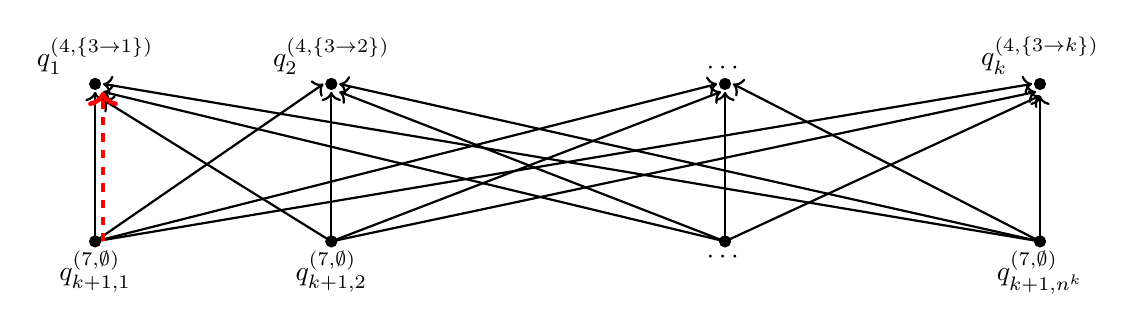
\begin{tikzpicture}
%%% The nodes represents the k query in the first round
\filldraw[black] (0, 2) circle (2pt) node [anchor=south]{$q_1^{(4, \{3 \to 1\} )}$};
\filldraw[black] (3, 2) circle (2pt) node [anchor=south]{$q_2^{(4, \{3 \to 2\} )}$};
% \filldraw[black] (6, 2) circle (2pt) node [anchor=south]{$q^4_3$};
\filldraw[black] (8, 2) circle (2pt) node [anchor=south]{$\cdots$};
\filldraw[black] (12, 2) circle (2pt) node [anchor=south]{$q_k^{(4, \{3 \to k\} )}$};
%%%%%% The nodes represents the n^k queries in the second round
\filldraw[black] (0, 0) circle (2pt) node [anchor=north]{$q_{k+1,1}^{(7, \emptyset)}$};
\filldraw[black] (3, 0) circle (2pt) node [anchor=north]{$q_{k+1,2}^{(7, \emptyset)}$};
% \filldraw[black] (6, 0) circle (2pt) node [anchor=north]{$q^{3, 7}_{k+1}$};
\filldraw[black] (8, 0) circle (2pt) node [anchor=north]{$\cdots$};
\filldraw[black] (12, 0) circle (2pt) node [anchor=north]{$q_{k+1,n^k}^{(7, \emptyset)}$};
%%%%%% The edges represents their dependency relations GROUP 1
\draw[ thick,->] (0, 0)  -- (0, 1.9) ;
\draw[ thick,->] (0, 0)  -- (2.9, 2) ;
% \draw[very thick,->] (0, 0)  -- (6, 2) ;
\draw[ thick,->] (0, 0)  -- (7.9, 2) ;
\draw[ thick,->] (0, 0)  -- (11.9, 2) ;
%%%%%% The edges represents their dependency relations GROUP 2
\draw[ thick,->] (3, 0)  -- (0.1, 1.8) ;
\draw[ thick,->] (3, 0)  -- (3, 1.9) ;
% \draw[very thick,->] (0, 0)  -- (6, 2) ;
\draw[ thick,->] (3, 0)  -- (7.95, 1.9) ;
\draw[ thick,->] (3, 0)  -- (11.95, 1.9) ;
%%%%%% The edges represents their dependency relations GROUP 3
\draw[ thick,->] (8, 0)  -- (0.1, 1.9) ;
\draw[ thick,->] (8, 0)  -- (3.1, 1.9) ;
% \draw[very thick,->] (0, 0)  -- (6, 2) ;
\draw[ thick,->] (8, 0)  -- (8, 1.9) ;
\draw[ thick,->] (8, 0)  -- (12, 1.85) ;
%%%%%% The edges represents their dependency relations GROUP 4
\draw[ thick,->] (12, 0)  -- (0.1, 2) ;
\draw[ thick,->] (12, 0)  -- (3.1, 2) ;
% \draw[very thick,->] (0, 0)  -- (6, 2) ;
\draw[ thick,->] (12, 0)  -- (8.1, 2) ;
\draw[ thick,->] (12, 0)  -- (12, 1.85) ;
%%%% The longest path representing the adaptivity
\draw[ultra thick, red, ->, dashed] (0.1, 0) -- (0.1, 1.9);
\end{tikzpicture}
}
\end{center}
\end{example}
%
\newpage

%
\begin{example}[Multi-Round Algorithm]
{
\[
MR \triangleq
\begin{array}{l}
    \left[i \leftarrow 1 \right]^1 ; \\
    \left[I \leftarrow [] \right]^2; \\
   \ewhile ~ [i < k]^{3} 
    \ ~ \edo ~ \\ \Big(
    \left[p \leftarrow c \right]^4 ; \\
    \left[a \leftarrow \query(p, I) \right]^5; \\
    \left[I \leftarrow \eupdt( {I}, (a, p))  \right]^6 ; \\
    \left[i \leftarrow i + 1 \right]^7 \\
    \Big) 
\end{array}
%
~~~~ \Rightarrow ~~~
%
MR^{ssa} \triangleq
\begin{array}{l}
    \left[i \leftarrow 1 \right]^1 ; \\
   \left[I \leftarrow [] \right]^2; \\
   \ewhile ~ [i < k]^{3} 0, [I_3,I_1,I_2] \\ 
    \ ~ \edo ~ \\ \Big(
    \left[p_1 \leftarrow c \right]^4 ; \\
    \left[a \leftarrow \query(p_1, I_2) \right]^5; \\
    \left[I_2 \leftarrow \eupdt( {I_3}, (a_1, p_1))  \right]^6;\\
    \left[i \leftarrow i + 1 \right]^7 \\
    \Big) 
\end{array}
\]
}
%
%
%
Adapt($MR$) = k.
\\
%
{
Using \THESYSTEM, we first generate a assigned variables $G$ from an empty list $[]$ and empty whlemap $\emptyset$.
 \[[]; \emptyset; MR^{ssa} \to G; w  \land w = \emptyset\].
 %
 \[
 G_{k=2} = 
 \left[
 i_1^{1}, I_1^2, i_3^3, I_3^3, p_1^4, a_1^5, I_2^6, i_2^7
\right] 
\]
  We denote $I_1^{1}$ short for ${I_1}^{(1,\emptyset)}$ and ${I_3}^{(2,1)}$ short for ${I_3}^{(2,[2:1])}$, where the label $(2, 1)$ represents at line number $2$ and in the $1$ st iteration.
  }
{
	\[
M =  \left[ \begin{matrix}
   i_1^{1} & I_1^2 & i_3^3 & I_3^3 & p_1^4 & a_1^5 & I_2^6 & i_2^7\\
 0 & 0 & 0 & 0 & 0 & 0 & 0 & 0 \\
 1 & 0 & 0 & 0 & 0 & 0 & 0 & 0 \\
 0 & 0 & 0 & 0 & 0 & 0 & 0 & 0 \\
 0 & 1 & 0 & 0 & 0 & 0 & 0 & 0 \\
 0 & 1 & 1 & 1 & 0 & 0 & 0 & 0 \\
 1 & 0 & 0 & 0 & 1 & 0 & 0 & 0 \\
 0 & 0 & 0 & 0 & 0 & 0 & 0 & 0 \\
 0 & 0 & 0 & 0 & 0 & 1 & 0 & 0 \\
 0 & 0 & 0 & 0 & 0 & 1 & 1 & 1 \\
 1 & 0 & 0 & 0 & 0 & 0 & 0 & 0  \\
 \end{matrix} \right] 
~ , V = \left [ \begin{matrix}
i_1^1 & 0 \\
I_1^2 & 0 \\
i_3^3 & 2 \\
I_3^3 & 2 \\
p_1^4 & 2 \\
a_1^5 & 1 \\
I_2^6 & 2 \\
i_2^7 & 2
\end{matrix} \right ]
\]
}

\newpage
\begin{center}
%
\todo{
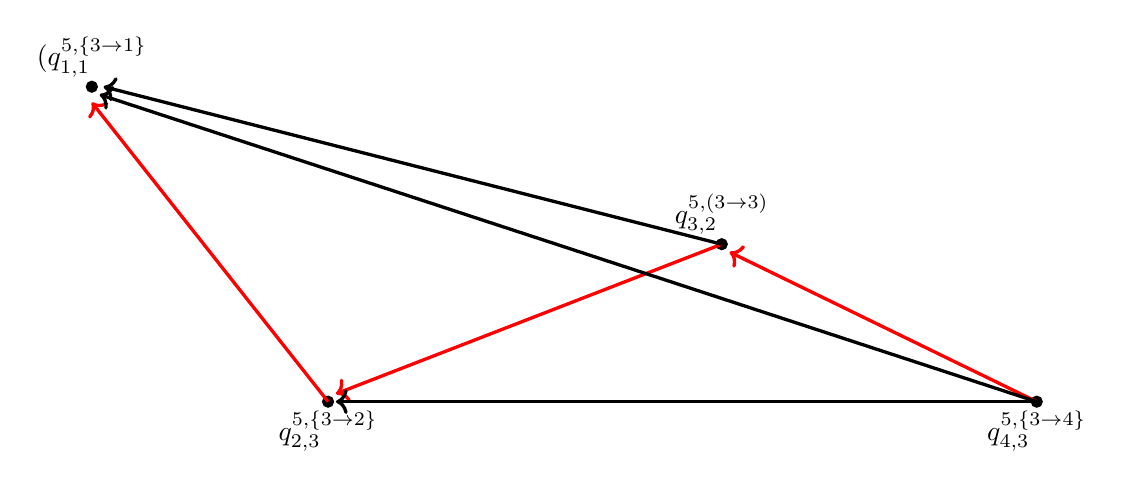
\begin{tikzpicture}
%%% The nodes represents the k query in the first round
\filldraw[black] (0, 4) circle (2pt) node [anchor=south]{$(q^{5, \{3 \to 1\}}_{1, 1}$};
\filldraw[black] (3, 0) circle (2pt) node [anchor=north]{$q^{5, \{3 \to 2\}}_{2, 3}$};
% \filldraw[black] (6, 0) circle (2pt) node [anchor=north]{$q^{3, 7}_{k+1}$};
% \filldraw[black] (8, 0) circle (2pt) node [anchor=north]{$\cdots$};
\filldraw[black] (12, 0) circle (2pt) node [anchor=north]{$q^{5, \{3 \to 4\}}_{4, 3}$};
\filldraw[black] (8, 2) circle (2pt) node [anchor=south]{$q^{5, (3 \to 3)}_{3, 2}$};
\draw[very thick,->, red] (3, 0)  -- (0, 3.8) ;
%
\draw[very thick,->, red] (8, 2)  -- (3.1, 0.1) ;
\draw[very thick,->] (8, 2)  -- (0.15, 4) ;
% \draw[very thick,->] (8, 0)  -- (3.1, 0) ;
% \draw[very thick,->] (8, 4)  -- (3, 0.2) ;
% %
%%%%%% The edges represents their dependency relations GROUP 4
% \draw[very thick,->] (0, 0)  -- (6, 2) ;
% \draw[very thick,->] (12, 2)  -- (8.1, 2) ;
\draw[very thick,->, red] (12, 0)  -- (8.1, 1.9) ;
\draw[very thick,->] (12, 0)  -- (3.1, 0) ;
\draw[very thick,->] (12, 0)  -- (0.1, 3.9) ;
%
\end{tikzpicture}
}
\end{center}
%
\newpage
%
$\forall k. \forall D$, we have $A(TR^L) = (k - 1)$ given all possible execution traces.
\todo{
\begin{center}
%
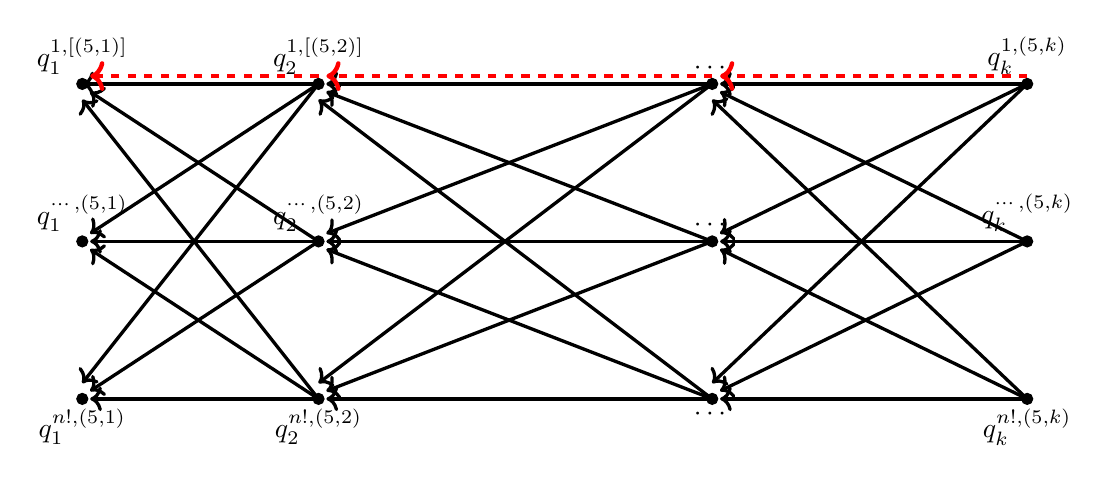
\begin{tikzpicture}
%%% The nodes represents the k query in the first round
\filldraw[black] (0, 4) circle (2pt) node [anchor=south]{$q^{1, [(5, 1)]}_1$};
\filldraw[black] (3, 4) circle (2pt) node [anchor=south]{$q^{1, [(5, 2)]}_2$};
% \filldraw[black] (6, 2) circle (2pt) node [anchor=south]{$q^4_3$};
\filldraw[black] (8, 4) circle (2pt) node [anchor=south]{$\cdots$};
\filldraw[black] (12, 4) circle (2pt) node [anchor=south]{$q^{1, (5, k)}_k$};
%%%%%% The nodes represents the n^k queries in the second round
\filldraw[black] (0, 0) circle (2pt) node [anchor=north]{$q^{n!, (5, 1)}_1$};
\filldraw[black] (3, 0) circle (2pt) node [anchor=north]{$q^{n!, (5, 2)}_2$};
% \filldraw[black] (6, 0) circle (2pt) node [anchor=north]{$q^{3, 7}_{k+1}$};
\filldraw[black] (8, 0) circle (2pt) node [anchor=north]{$\cdots$};
\filldraw[black] (12, 0) circle (2pt) node [anchor=north]{$q^{n!, (5, k)}_k$};
%%% The nodes represents the k query in the first round
\filldraw[black] (0, 2) circle (2pt) node [anchor=south]{$q^{\cdots, (5, 1)}_1$};
\filldraw[black] (3, 2) circle (2pt) node [anchor=south]{$q^{\cdots, (5, 2)}_2$};
% \filldraw[black] (6, 2) circle (2pt) node [anchor=south]{$q^4_3$};
\filldraw[black] (8, 2) circle (2pt) node [anchor=south]{$\cdots$};
\filldraw[black] (12, 2) circle (2pt) node [anchor=south]{$q^{\cdots, (5, k)}_k$};
%%%%%% The edges represents their dependency relations GROUP 1
\draw[very thick,->] (3, 2)  -- (0.1, 2) ;
\draw[very thick,->] (3, 0)  -- (0.1, 1.9) ;
\draw[very thick,->] (3, 4)  -- (0.1, 2.1) ;
%
\draw[very thick,->] (3, 2)  -- (0.1, 0.1) ;
\draw[very thick,->] (3, 0)  -- (0.1, 0) ;
\draw[very thick,->] (3, 4)  -- (0, 0.2) ;
%
\draw[very thick,->] (3, 2)  -- (0.1, 3.9) ;
\draw[very thick,->] (3, 0)  -- (0, 3.8) ;
\draw[very thick,->] (3, 4)  -- (0, 4) ;
% \draw[very thick,->] (0, 0)  -- (6, 2) ;
%%%%%% The edges represents their dependency relations GROUP 2
% \draw[very thick,->] (0, 0)  -- (6, 2) ;
\draw[very thick,->] (8, 2)  -- (3.1, 2) ;
\draw[very thick,->] (8, 0)  -- (3.1, 1.9) ;
\draw[very thick,->] (8, 4)  -- (3.1, 2.1) ;
%
\draw[very thick,->] (8, 2)  -- (3.1, 0.1) ;
\draw[very thick,->] (8, 0)  -- (3.1, 0) ;
\draw[very thick,->] (8, 4)  -- (3, 0.2) ;
%
\draw[very thick,->] (8, 2)  -- (3.1, 3.9) ;
\draw[very thick,->] (8, 0)  -- (3, 3.8) ;
\draw[very thick,->] (8, 4)  -- (3.1, 4) ;
%%%%%% The edges represents their dependency relations GROUP 4
% \draw[very thick,->] (0, 0)  -- (6, 2) ;
\draw[very thick,->] (12, 2)  -- (8.1, 2) ;
\draw[very thick,->] (12, 0)  -- (8.1, 1.9) ;
\draw[very thick,->] (12, 4)  -- (8.1, 2.1) ;
%
\draw[very thick,->] (12, 2)  -- (8.1, 0.1) ;
\draw[very thick,->] (12, 0)  -- (8.1, 0) ;
\draw[very thick,->] (12, 4)  -- (8, 0.2) ;
%
\draw[very thick,->] (12, 2)  -- (8.1, 3.9) ;
\draw[very thick,->] (12, 0)  -- (8, 3.8) ;
\draw[very thick,->] (12, 4)  -- (8.1, 4) ;
%
%%%% The longest path representing the adaptivity
\draw[ultra thick, red, ->, dashed] (3, 4.1)  -- (0.1, 4.1);
\draw[ultra thick, red, ->, dashed] (8, 4.1)  -- (3.1, 4.1);
\draw[ultra thick, red, ->, dashed] (12, 4.1)  -- (8.1, 4.1);
\end{tikzpicture}
\end{center}
}
\end{example}
%%
%%
\section{Non Determinism}
%%
\paragraph{Non-Determinism of queries.}
% 
{
When evaluating a query $\query(\qval)$ on a given database $D$, 
in addition to obtain a result $v$ from the database $v = \query(\qval)(D)$,
we assume there is an underlying mechanism that will perform extra manipulations on $v$. 
The mechanism is considered as primitive operations in our language, behaving as black box to programmers.
There are different kinds of mechanisms, 
such as adding noise sampled from certain probabilistic distribution to the result \cite{dwork2015preserving}.
Because of the randomness of the underlying mechanism, the evaluation of a query $\query(\qval)$ is non-deterministic. 
That's the reason, in the Definition \ref{def:query_dep}, given a fixed database $D$, there will be a query domain $\qdom$ where $\query(\qval)(D) $ can be evaluated to different values $v \in \qdom$.
}
\\
{
On the other hand, in the operational semantics rule \textbf{query-v}:
\[
		\inferrule
	{
	\query(\qval) = v
	}
	{
	\config{m, [\assign{x}{\query(\qval)}]^l, t, w} 
	\xrightarrow{} 
	\config{m[ v/ x], \eskip,  (t ++ [(\qval, l, w)],w }
	}
	~\textbf{query-v}
	\]
, we evaluate the query given database $D$ based on an assumption that the underlying mechanism is fixed.
This fixed mechanism only adds constant $0$ to the original result $v$ returned from the database, i.e., $v = \query(\qval)(D)$. 
}
%
\\
%
The Lemma \ref{lem:semidetrm} and \ref{lem:querysemidetrm} formalize this property.
%
\begin{lem}
[Semi-Determinism].
\label{lem:semidetrm}\\
{
for any program $c$ with a starting memory $m$, trace $t$ and while label $w$, 
if program $c$ contains neither  
$[\assign{x}{\query(\qexpr)}]^l$ nor $[\assign{x}{\query(\qval)}]^l$ for any $\qexpr$ and $\qval$, then
%
$$
\bigwedge
\left\{\begin{array}{l}
\config{m, c, t, w} 
\rightarrow^{*} 
\config{m_1, \eskip, t_1, w_1} 
\\ 
\config{m, c, t, w} 
\rightarrow^{*} 
\config{m_2, \eskip, t_2, w_2} 
\end{array}
\right\}
\implies
(m_1 = m_2 \land t_1 = t_2 \land w_1 = w_2)
 $$ 
}
\end{lem}
%
\begin{proof}
{
Proof is obvious by induction on the operational semantics rules.
}
\end{proof}
%
%
\begin{lem}
[Query Semi-Determinism].
\label{lem:querysemidetrm}
\\
{
Given a program $c; \assign{x}{\query(\qexpr)}; c'$ with a starting memory $m$, trace $t$ and while label $w$, 
s.t. $c$ contains neither  
$[\assign{x}{\query(\qexpr)}]^l$ nor $[\assign{x}{\query(\qval)}]^l$ for any $\qexpr$ and $\qval$, then:
%
\[
\bigwedge
\left\{
\begin{array}{l}
\config{m, c; \assign{x}{\query(\qexpr)}; c', t, w} 
\rightarrow^{*} 
\config{m_1, \assign{x}{\query(\qval_1)}; c', t_1, w_1} 
\\
\config{m, c; \assign{x}{\query(\qexpr)}; c', t, w} 
\rightarrow^{*} 
\config{m_2, \assign{x}{\query(\qval_2)}; c', t_2, w_2} 
\end{array}
\right\}
\implies
(\qval_1 = \qval_2 \land m_1 = m_2 \land t_1 = t_2 \land w_1 = w_2)
\]
}
\end{lem}
%
\begin{proof}
{
Proof is obvious by induction on the operational semantics rules.
}
\end{proof}
% %
\section{Analysis of Generalization Error}

\begin{example}[Two Round Algorithm]
\[
TR^H(k) \triangleq
{
\begin{array}{l}
    % \left[j \leftarrow 0 \right]^1 ; \\
    \clabel{a_1 \leftarrow [] }^1; \\
    \eloop ~ [k]^{2} ~ (a_2 \leftarrow f(1, a_1, a_3)) \\
    ~ \edo ~ \\
    \Big(
     \clabel{x_1 \leftarrow \query() }^3 ; \\
    \clabel{a_3 \leftarrow x_1 :: a_2 }^4     \Big);\\
    \clabel{l \leftarrow q_{k + 1}(a_3)}^{5}\\
\end{array}
}
\]
\end{example}
%
\begin{example}[Multi-Round Algorithm]
\[
MR^H \triangleq
\begin{array}{l}
    %  \left[j \leftarrow 0 \right]^1 ; \\
    \left[I_2 \leftarrow [] \right]^1; \\
    \eloop ~ [k]^{2} ~ (I_2 \leftarrow f(2, I_1, I_3)) \\ 
    \ ~ \edo ~ \\ \Big(
    \left[p_1 \leftarrow c \right]^3 ; \\
    \left[a_1 \leftarrow \delta(\query(p, I_2)) \right]^4; \\
    \left[I_3 \leftarrow \eupdt( {I_2}, (a_1, p))  \right]^5
    \Big) 
\end{array}
\]
\end{example}
%
%
By applying different mechanisms $\delta()$ over the queries $\query(\cdot)$, we have different error bounds.
\\
\textbf{Gaussian Mechanism:} $N(0, \sigma)$ \cite{dwork2015preserving}:
\\
Adaptivity $r = 2$: 
$ \sigma = O \left(\frac{\sqrt{r \log(k)}}{\sqrt{n}} \right)$ (also known as expected error);
\\
Adaptivity unknown:
$ \sigma = O\left(\frac{\sqrt[4]{k}}{\sqrt{n}} \right)$;
\\
{Mean Squared Error Bound:} 
$ \frac{1}{2n} \min\limits_{\lambda \in [0, 1]}
\left( \frac{2\rho k n - \ln(1 - \lambda)}{\lambda} 
\right)
+ 2 \mathbb{E}_{Z_i \sim N(0, \frac{1}{2n^2 \rho})}
\left[ \max\limits_{i \in [k]} (Z_i^2) \right]$
%
\\
{Confidence Bounds:} minimize $\tau$ where
$\tau \geq \sqrt{\frac{2}{n \beta}
\min\limits_{\lambda \in [0, 1]}
\left( \frac{2\rho k n - \ln(1 - \lambda)}{\lambda} 
\right)
}$
and 
$\tau \geq \frac{2}{n} \sqrt{\frac{\ln(4n /\beta}{\rho'}}$ with confidence level $1 - \beta$ .
\\
\textbf{$(\epsilon, \delta)-DP$ mechanism}:
\\
Confidence Bounds:
$\tau \geq \sqrt{\frac{48}{n} \ln(4/\beta) }$ with $\epsilon \leq \frac{\tau}{4}$ and $\delta = 
\exp \left(\frac{-4 \ln (8/\beta)}{\tau} \right)$
\\
\textbf{Sample Splitting}: 
\\
Expected Error: $O \left(\frac{\sqrt{k \log(k)}}{\sqrt{n}} \right)$
\\
\textbf{Thresholdout}: $B, \sigma, T, h$ 
\\
Confidence bounds:  
$\tau = \max\limits\left\{ 
\sqrt{\frac{2\zeta }{h \beta}},
2\sigma \ln(\frac{\beta}{2}),
\sqrt{\frac{1}{\beta}} \cdot \left(\sqrt{T^2 + 56\sigma^2} + \sqrt{\frac{\zeta}{4h} } \right)
\right\}
$,
for $\zeta = \min\limits_{\lambda \in [0, 1)}
\left( \frac{2B \ (\sigma^2 h) - \ln(1 - \lambda)}{\lambda} \right)$

\clearpage


% \section{new \THESYSTEM with loop }
\subsection{Analysis Rules/Algorithms of \THESYSTEM}

There are two steps for our algorithm to get the estimation of the adaptivity of a program $\ssa{c}$ in the ssa form. 
\begin{enumerate}
    \item Estimate the variables that are new generated (via assignment) and store these variables in a global list $G$. We have the algorithm of the form : $\ag{ G;w; \ssa{c}}{G';w'} $.
    \item We start to track the dependence between variables in a matrix $M$, whose size is $|G| \times |G|$, and track whether arbitrary variable is assigned with a query result in a vector $V$ with size $|G|$. The algorithm to fill in the matrix is of the form: $\ad{\Gamma ; \ssa{c} ; i_1}{M;V;{i_2}}$. $\Gamma$ is a vector records the variables the current program $\ssa{c}$ depends on, the index $i_1$ is a pointer which refers to the position of the first new-generated variable in $\ssa{c}$ in the global list $G$, and $i_2$ points to the first new variable that is not in $\ssa{c}$ (if exists). 
\end{enumerate}

% We have the judgment of the form $\vdash^{i_1, i_2}_{M,V} ~ c  $.  Our grade is a combination of a matrix $M$, used to track the dependency of variables appeared in the statement $c$, and a vector $V$ indicating the variables associated with results from queries $q$. The size of the matrix $M$ is $L \times L$, and vector $V$ of size $L$, where $L$ is the total size of variables needed in the program $c$, which is fixed per program. We assume the program is in the style of Static Single Assignment.To be more specific, we give a quick example: $x \leftarrow e_1; x \leftarrow e_2 $ will be rewritten as $ x_1 \leftarrow e_1; x_2 \leftarrow e_2$. And the if condition $ \eif ~ e_b \ethen x \leftarrow e_1 \eelse x \leftarrow e_2  $ will look like $ \eif ~ e_b \ethen x_1 \leftarrow e_1 \eelse x_2 \leftarrow e_2  $. As we have seen, SSA requires unique variables, and these newly generated variables will be recorded in the matrix $M$.  Also, the variable at different iteration is treated as different variable in the matrix $M$ and vector $V$.

% The superscript $i_1,i_2$  specify the range of "living" or "active" variables in the matrix and vector. $i_1$ is the starting line (and column) in the matrix where the new generated variables in program $c$ starts to show up. Likewise, $i_2$ states the ending position of active range by $c$.
%  Worth to mention, $i_1,i_2$ can be used to track the exact location of newly generated variables. For example, the assignment statement $x \leftarrow e$ or $x \leftarrow q $ with $c_2 =c_1+1$, tells us the variable $x$ is at the $c_1$th line(column) of the matrix. As we can notice, the loop increases the variables needed in the matrix by $N \times a$ where $N$ is the number of rounds of the loop and $a$ is the size of the variables generated in the loop body. We will have a global map, which maps the variable name to the position in the vector. We call it $GM: VAR \to \mathbb{N}$.

We give an example of $M$ and $V$ of the program $c$.   
$$
c= \begin{array}{c}
\ssa{\assign {x_1} {q}} ;        \\
\ssa{\assign {x_2} {x_1+1}} ;\\
\ssa{\assign {x_3} {x_2+2} }
\end{array}~~~~~~~~~~~~
M =  \left[ \begin{matrix}
 & (x_1) & (x_2) & (x_3) \\
(x_1) & 0 & 0 & 0 \\
(x_2) & 1 & 0 & 0 \\
(x_3) & 1 & 1 & 0 \\
\end{matrix} \right] ~ , V = \left [ \begin{matrix}
(x_1) &  1 \\
(x_2) & 0 \\
(x_3) & 0 \\
\end{matrix} \right ]
$$
Still use the program $c$ as the example, the global list $G$ is now : $ [ x_1 , x_2 , x_3] $. 
The function $\mathsf{Left}$ and $\mathsf{Right}$ is used to generate the corresponding vector of the left side and right side of an assignment. Take $\assign {x_2} {x_1+1} $ as an example, the result is shown as follows.
\[
\sf{L}(1) = \left[ \begin{matrix}
 0  & ~~~(x_1) \\
 1 & ~~~(x_2) \\
 0 & ~~~(x_3) \\
\end{matrix}   \right ] ~~~~~~~~~~~~~~
\sf{R} (x_1+1, 1) = \left[ \begin{matrix} 
   1 & 0 & 0 \\
   (x_1) & (x_2) & (x_3) \\
\end{matrix}  \right]
\]
Now let us think about the loop.
\[\ssa{c_3} \triangleq
\begin{array}{l}
     \left[\ssa{ x_1 \leftarrow q_1}  \right]^1 ; \\
    \eloop ~ [2]^{2} , 0,\\
  \ssa{[x_3 , x_1 , x_2]} 
     ~ \edo
    \\
    ~ \Big( 
    \left[\ssa{ y_1 \leftarrow q_2} \right]^3; \\
    \left[\ssa{x_2 \leftarrow y_1  + x_3 } \right]^5
    \Big) ; \\
     \left[ \assign{z_1}{x_3 + 2}  \right]^{6}
\end{array}
~~~~~~~~~~~~
M =  \left[ \begin{matrix}
 & (x_1) & (x_3^{1}) & (y_1^{1}) & (x_3^{1})  & (x_3^{2}) & (y_1^{2}) & (x_2^{2}) & (x_3^{f}) &  (z_1) \\
(x_1) & 0 & 0 & 0 & 0 & 0 & 0 & 0 &0 &0 \\
(x_3^{1}) & 1 & 0 & 0 & 0 & 0 & 0 & 0&0&0\\
(y_1^{1}) & 0 & 0 & 0 & 0 & 0 & 0& 0& 0 &0\\
(x_2^{1}) & 0 & 1 & 1 & 0 & 0 & 0 & 0& 0&0\\
(x_3^{2}) & 0 & 0 & 0 & 1 & 0 & 0 & 0 & 0&0 \\
(y_1^{2}) & 0 & 0 & 0 & 0 & 0 & 0 & 0& 0&0\\
(x_2^{2}) & 0 & 0 & 0 & 0 & 1 & 1 & 0& 0&0\\
(x_3^{f}) & 1 & 0 & 0 & 0 & 0 & 0 & 1& 0&0\\
(z_1) & 0 & 0 & 0 & 0 & 0 & 0 & 0 & 1 &0 \\
\end{matrix} \right] ~ , V = \left [ \begin{matrix}
(x_1) &  1 \\
(x_3^{1}) & 0 \\
(y_1^{1}) & 1 \\
(x_2^{1}) &  0 \\
(x_3^{2}) & 0 \\
(y_1^{2}) & 1 \\
(x_2^{2}) &  0 \\
(x_3^{f}) &  0 \\
(z_1) &  0 \\
\end{matrix} \right ]
\]

\[\ssa{c_3'} \triangleq
\begin{array}{l}
     \left[\ssa{ x_1 \leftarrow q_1}  \right]^1 ; \\
    \eloop ~ [0]^{2} , 0,\\
  \ssa{[x_3 , x_1 , x_2]} 
     ~ \edo
    \\
    ~ \Big( 
    \left[\ssa{ y_1 \leftarrow q_2} \right]^3; \\
    \left[\ssa{x_2 \leftarrow y_1  + x_3 } \right]^5
    \Big) ; \\
    \left[ \assign{z_1}{x_3 + 2}  \right]^{6}
\end{array}
~~~~~~~~~~~~
M =  \left[ \begin{matrix}
 & (x_1) & (x_3^{f}) & (z_1)  \\
(x_1) & 0 & 0 & 0 \\
(x_3^{f}) & 1 & 0 & 0 \\
(z_1^{2}) & 0 & 1 & 0 \\
\end{matrix} \right] ~ , V = \left [ \begin{matrix}
(x_1) &  1 \\
(x_3^{f}) & 0 \\
(z_1) &  0 \\
\end{matrix} \right ]
\]
We can now look at the if statement.
\[ c_4 \triangleq
\begin{array}{l}
   \left[ x \leftarrow q_1 \right]^1; \\
   \left[y \leftarrow q_2\right]^2 ; \\
    \eif \;( x + y == 5 )^3\; \\
    \mathsf{then} \;\left[ x \leftarrow q_3 \right]^4 \; \\
    \mathsf{else} (\;\left[ x \leftarrow q_4 \right]^5 ; \\
    y \leftarrow 2 ) ;\\
   \left[ z \leftarrow x +y \right]^6; \\
\end{array}
\hspace{20pt} \hookrightarrow \hspace{20pt}
%
 \ssa{c_4} \triangleq
\begin{array}{l}
   \left[ \ssa{ x_1 \leftarrow q_1} \right]^1; \\
   \left[\ssa{ y_1 \leftarrow q_2} \right]^2 ; \\
    \eif \;( \ssa{ x_1 + y_1 == 5} )^3, [ x_4,x_2,x_3 ],[] ,[y_3,y_1,y_2 ]\; \\
    \mathsf{then} \;\left[ \ssa{ x_2 \leftarrow q_3}\right]^4 \; \\
    \mathsf{else} (\;\left[ \ssa{x_3 \leftarrow q_4} \right]^5 ; \\
     \ssa{y_2 \leftarrow 2} ) \\
   \left[ \ssa{ z_1 \leftarrow x_4 +y_3 }\right]^6; \\
\end{array}
\]
\[
M_{c4} =  \left[ \begin{matrix}
 & (x_1) & (y_1) & (x_2) & (x_3)  & (y_2) & (x_4) & (y_3) & (z_1)  \\
(x_1) & 0 & 0 & 0 & 0 & 0 & 0 & 0 &0  \\
(y_1) & 0 & 0 & 0 & 0 & 0 & 0 & 0&0\\
(x_2) & 0 & 0 & 0 & 0 & 0 & 0& 0& 0 \\
(x_3) & 0 & 0 & 0 & 0 & 0 & 0 & 0& 0\\
(y_2) & 0 & 0 & 0 & 0 & 0 & 0 & 0 & 0 \\
(x_4) & 0 & 0 & 1 & 1 & 0 & 0 & 0 &0\\
(y_3) & 0 & 1 & 0 & 0 & 1 & 0 & 0 &0\\
(z_1) & 0 & 0 & 0 & 0 & 0 & 1 & 1 & 0  \\
\end{matrix} \right] ~ , V_{c4} = \left [ \begin{matrix}
(x_1) &  1 \\
(y_1) & 1 \\
(x_2) & 1 \\
(x_3) &  1 \\
(y_2) & 0 \\
(x_4) & 0 \\
(y_3) &  0 \\
(z_1) &  0 \\
\end{matrix} \right ]
\]
% We consider to have the superscript to denote the iteration number (or map if we have nested loop), as shown in the above matrix and vector. The global map $G$ is generated by analysing the program. We can estimate the variables needed in the loop by using the loop number $N$ and the loop body. In this example, the global map for $c_3$ : $ \{ x_1 \to 1, x_2^{1} \to 2, y_1^{1} \to 3 , x_3^{1} \to 4 , x_2^{2} \to 5 , y_1^{2} \to 6 , x_3^{2} \to 7  \} $.  
% By default, $G(x_2)$ gives the location for the first appearance of the variable $x_2$. We can also allow $G(x_2 , 2)$ to get the location of the second iteration $x_2^{2}$. We also allow $G(x, i, i+n)$ to return a set of locations where $x$ appears in the vector in the certain range $[i, i+n]$, which helps to locate variables in the loop.




% Also, to be able to track the relation between variables in varied iterations in the loop. we define a dependent map $\mathsf{DM}$ based on command $c$ to provide the dependency relation(syntactically) between variables. $\mathsf{VAR}(\expr)$ gives the set of variables appears in the expression $\expr$.
% \[
% \begin{array}{lll}
% \mathsf{DM} (c_1; c_2) & \triangleq &  \mathsf{DM} (c_1) \uplus \mathsf{DM} (c_2)  \\
% \mathsf{DM} (x_1 \leftarrow \expr ) & \triangleq & \{  x_1 \to \mathsf{VARS}(\expr)  \}
% \end{array}
% \]

\subsection{The algorithm to estimate the matrix and vector}
We first generate a list of variables $G$ that will be assigned with values (via the command $\assign{x}{e}$ or $\assign{x}{q}$). 

 \begin{mathpar}
\inferrule
{
}
{ \ag{G ;w; \ssa{[\assign {x}{\expr}]^{l}}}{G ++ [\ssa{x}^{(l,w)}];w}
% G ;w; \ssa{[\assign {x}{\expr}]^{l}} \to G ++ [x^{(l,w)}];w 
}
~\textbf{ag-asgn}
\and
\inferrule
{
}
{ \ag{G ;w;  [ \assign{\ssa{x}}{q(\ssa{\expr})}]^{l}}{  G ++ [\ssa{x}^{(l,w)}] ; w} 
}~\textbf{ag-query}
%
\and 
%
\inferrule
{
\ag{G; w; \ssa{c_1}}{  G_1;w_1}
\and 
 \ag{G_1;w ; \ssa{c_2}}{  G_2; w_2}
 \\
 {G_3 = G_2 ++ \ssa{[\bar{x}^{(l,w)}]++ \ssa{[\bar{y}^{(l,w)}]}++ \ssa{[\bar{z}^{(l,w)}]} }}
}
{
\ag{G; w;
[\eif(\ssa{\bexpr},[ \bar{\ssa{x}}, \bar{\ssa{x_1}}, \bar{\ssa{x_2}}] ,[ \bar{\ssa{y}}, \bar{\ssa{y_1}}, \bar{\ssa{y_2}}],[ \bar{\ssa{z}}, \bar{\ssa{z_1}}, \bar{\ssa{z_2}}], \ssa{ c_1, c_2)}]^{l} }{ G_3 ;w}
}~\textbf{ag-if}
%
%
%
\and 
%
\inferrule
{
\ag{G; w; \ssa{c_1}}{ G_1; w_1}
\and 
\ag{G_1;w_1; \ssa{c_2}}{ G_2; w_2}
}
{
\ag{G; w;
\ssa{(c_1 ; c_2)}}{  G_2 ; w_2}
}
~\textbf{ag-seq}
\and 
\inferrule
{
{G_0 = G \quad w_0 =w }
\and
\forall 0 \leq z < N. 
{ \ag{ G_z ++ \ssa{[\bar{x}^{(l, {w_z}+l)}]} ; (w_z+l); \ssa{c}}{ G_{z+1} ; w_{z+1}}  }
\\
{G_f = G_N ++ \ssa{[\bar{x}^{(l, w_N \setminus l)}]} }
\and
{ \ssa{\aexpr} =  {N}  }
}
{\ag{G; w; [\eloop ~ \ssa{\aexpr}, n, [\bar{\ssa{x}}, \bar{\ssa{x_1}}, \bar{\ssa{x_2}}] ~ \edo ~ \ssa{c}]^{l} }{ G_f; w_N\setminus l }
}~\textbf{ag-loop}
\end{mathpar}


%
%
% \paragraph{Analysis Rules.}
% \[\begin{array}{ll}
%     \mathcal{A}( \assign x \expr )( \Gamma , i )  & =  ( \mathsf{L}(x) * ( \mathsf{R}(\expr) + \Gamma ), V, i+1 )\\
%     \mathcal{A}( \assign x q)( \Gamma ,  i )  & = ( \mathsf{L}(x) * ( \mathsf{R}(\emptyset) + \Gamma) , \mathsf{L}(x) , i+1 )\\
%     \mathcal{A}( \eif ~ e_b \ethen c_1 \eelse c_2 )( \Gamma , i ) & =   \elet \; (M_1, v_1, i_1) =  \mathcal{A}(C_1)(\Gamma +\mathsf{R}(e_b) , i)
%     \ein \; \\
%     &  \elet \;  (M_2, v_2, i_2)= \mathcal{A}(C_2) (\Gamma +\mathsf{R}(e_b) ,i_1) \ein \; \\
%     & (  M_1 \uplus M_2, V_1 \uplus V_2   , i_2 )
%     \\
%     \mathcal{A}( c_1 ; c_2 )( \Gamma ,  i )  & =  \elet \;     (M_1, v_1, i_1) = 
%     \mathcal{A}(c_1) (\Gamma  +\mathsf{R}(e_b) , i)
%     \ein \; \\
%     &  \elet \;  (M_2, v_2, i_2) =                      \mathcal{A}(c_2)(\Gamma +\mathsf{R}(e_b) ,
%       i_1) \ein \; \\ 
%       & (  M_1 \cdot M_2, V_1 \uplus V_2   , i_2 )    \\
%      \mathcal{A}( \eloop ~ \expr_N ~ (c_1) ~ \edo ~ c_2  )( \Gamma ,  i )  & =  \elet \;     (M_1, v_1, i+a) = 
%     \mathcal{A}(c_1;c_2 ) (\Gamma , i)
%     \ein \; \\
%     & ( M_{i,a}^N(c_1), V_{i, a}^N , i + N*a ) \\
%  \mathcal{A}( \eswitch(\expr, x,(v_j \rightarrow q_j )  )( \Gamma ,  i+j )  & =  \elet \;     (M_j, v_j, i+j) = 
%     \mathcal{A}(x_j \leftarrow q_j ) (\Gamma + \mathsf{R}(e), i+j-1)     
%   \ein \\
%   & ( \sum_{j=0}^{N} M_j, \sum_{j=0}^{N} V_j, i + N ) \quad j \in \{1, \dots, N\}  \\
%     \end{array}
% \]
%
%
\paragraph{Analysis Logic Rules.}
%
%
$\Gamma$ is a matrix of one row and $N$ columns, $N = |G|=|V|$.\\ 

$\mathsf{L(i)}$ generates a matrix of one column, $N$ rows, where the $i-th$ row is $1$, all the other rows are $0$.\\

$\mathsf{R(e, i)}$ generates a matrix of one row and $N$ columns, where the locations of variables in $e$ is marked as $1$. To handle loop, for instance, the variable $y$ appears many times in $G$, the argument $i$ helps to find the location of the current living variable $y$ in the expression $e$, which is the latest $y$ with the largest location $i_y< i$ in our global variable list $G$.\\ 


{$ \forall 0 \leq z < |\bar{x}|. \bar{x}(z) = x_z, \bar{x_1}(z) = x_{1z}, \bar{x_2}(z) = x_{2z} $ } \\

$ \Gamma \vdash_{M,v_{\emptyset}}^{i, i+ |\ssa{\bar{x}}|} \ssa{[ \bar{x},\bar{x_1},\bar{x_2}   ]} \triangleq { \forall 0 \leq z < |\bar{x}|.  \Gamma \vdash_{M_{x_z}, V_{\emptyset}}^{i+z, i+z+1 } x_z \leftarrow x_{1z} + x_{2z} }$ where $M = \sum_{z\in [|\bar{x}|] }M_{x_z} $\\

\framebox{$ {\Gamma} \vdash^{i_1, i_2}_{M,V} ~ c $}
%
% \begin{mathpar}
% \inferrule
% {M = \mathsf{L}(i) * ( \mathsf{R}(\expr,i) + \Gamma )
% }
% {\Gamma \vdash_{M, V_{\emptyset}}^{(i, i+1)} [\assign {\ssa{x}}{\ssa{\expr}} ]^{l}
% }
% ~\textbf{asgn}
% \and
% \inferrule
% {M = \mathsf{L}(i) * ( \Gamma)
% \\
% V= \mathsf{L}(i)
% }
% { \Gamma \vdash^{(i, i+1)}_{M, V} [ \assign{\ssa{x}}{q} ]^{l} 
% }~\textbf{query}
% %
% \and 
% %
% \inferrule
% {
% \Gamma + \mathsf{R}(\bexpr, i_1) \vdash^{(i_1, i_2)}_{M_1, V_1} \ssa{c_1} 
% % : \Phi \land \bexpr \Rightarrow \Psi
% \and 
% \Gamma + \mathsf{R}(\bexpr, i_1) \vdash^{(i_2, i_3)}_{M_2, V_2} \ssa{c_2} 
% % : \Phi \land \neg \bexpr \Rightarrow \Psi
% \\
% { \forall 0 \leq j < |\bar{x}|. \bar{x}(j) = x_j, \bar{x_1}(j) = x_{1j}, \bar{x_2}(j) = x_{2j}  }
% \\
% { \forall 0 \leq j < |\bar{x}|.  \Gamma \vdash_{M_{x_j}, V_{\emptyset}}^{i_3+j, i_3+j+1 } x_j \leftarrow x_{1j} + x_{2j} }
% \and
% { \forall 0 \leq j < |\bar{y}|.  \Gamma \vdash_{M_{y_j}, V_{\emptyset}}^{i_3+|\bar{x}|+j, i_3+|\bar{x}|+j+1 } y_j \leftarrow y_{1j} + y_{2j} }
% \\
% { \forall 0 \leq j < |\bar{z}|.  \Gamma \vdash_{M_{z_j}, V_{\emptyset}}^{i_3+|\bar{x}|+|\bar{y}|+j, i_3+|\bar{x}|+|\bar{y}|+j+1 } z_j \leftarrow z_{1j} + z_{2j} }
% \and
% {M = (M_1+M_2)+ \sum_{j\in [|\bar{x}|] }M_{x_j} + \sum_{j\in [|\bar{y}|] }M_{y_j} + \sum_{j\in [|\bar{z}|] }M_{z_j} }
% }
% {
% \Gamma \vdash^{(i_1, i_3+|\bar{x}|+|\bar{y}|+|\bar{z}|)}_{M, V_1 \uplus V_2 } 
% [\eif(\sbexpr,[ \bar{\ssa{x}}, \bar{\ssa{x_1}}, \bar{\ssa{x_2}}] ,[ \bar{\ssa{y}}, \bar{\ssa{y_1}}, \bar{\ssa{y_2}}] , [ \bar{\ssa{z}}, \bar{\ssa{z_1}}, \bar{\ssa{z_2}}] , \ssa{ c_1, c_2)}]^{l}
% }~\textbf{if}
% %
% %
% %
% \and 
% %
% \inferrule
% {
% \Gamma \vdash^{(i_1, i_2)}_{M_1, V_1} \ssa{c_1} 
% % : \Phi \Rightarrow \Phi_1
% \and 
% \Gamma \vdash^{(i_2, i_3)}_{M_2, V_2} \ssa{c_2} 
% % : \Phi_1 \Rightarrow \Psi 
% }
% {
% \Gamma \vdash^{(i_1, i_3)}_{M_1 \green{;} M_2, V_1 \uplus V_2}
% \ssa{c_1 ; c_2} 
% % : \Phi \Rightarrow \Psi
% }
% ~\textbf{seq}
% \and 
% \inferrule
% {
% B= |\ssa{\bar{x}}| 
% \and
% {\Gamma \vdash^{(i, i+B)}_{M_{10}, V_{10}} [\bar{\ssa{x}}, \bar{\ssa{x_1}}, \bar{\ssa{x_2}}] }
% \and
% {\Gamma \vdash^{(i+B,i+B+A )}_{M_{20}, V_{20}} \ssa{c} 
% }
% \\
% \forall 1 \leq j < N. 
% {\Gamma \vdash^{(i+j*(B+A), i+B+j*(B+A))}_{M_{1j}, V_{1j}}  } [\bar{\ssa{x}}, \bar{\ssa{x_1}}, \bar{\ssa{x_2}}]
% \and
% {\Gamma \vdash^{(i+B+j*(B+A),i+B+A+j*(B+A) )}_{M_{2j}, V_{2j}} \ssa{c} 
% % : \Phi \land e_n = \lceil{z+1}\rceil \Rightarrow \Psi 
% }
% \\
% {\Gamma \vdash^{(i+N*(B+A) ,i+N*(B+A)+B )}_{M, V} [\bar{\ssa{x}}, \bar{\ssa{x_1}}, \bar{\ssa{x_2}}]
% % : \Psi \Rightarrow \Phi \land e_N = \lceil{z}\rceil 
% }
% \and
% { \ssa{a} = \lceil {N} \rceil }
% \and
% {M' = M+ \sum_{0 \leq j <N} M_{1j}+M_{2j}  }
% \and
% {V' = V \uplus \sum_{0 \leq j <N} V_{1j} \uplus V_{2j}  }
% }
% {\Gamma \vdash^{(i, i+N*(B+A)+B   )}_{M', V'} 
% [\eloop ~ \ssa{\aexpr}, 0, [\bar{\ssa{x}}, \bar{\ssa{x_1}}, \bar{\ssa{x_2}}] ~ \edo ~ \ssa{c}]^{l}
% % : \Phi \land \expr_N = \lceil { N} \rceil \Rightarrow \Phi \land \expr_N = \lceil{0}\rceil
% }~\textbf{loop}
% % \and 
% % \inferrule
% % {
% % \Gamma \vdash^{(i,i+a )}_{M, V} c 
% % }
% % {\Gamma \vdash^{(i, i+ N*a)}_{M_{i,a}^N(f), V_{i, a}^N} 
% % \ewhile([\bexpr]^l,   c) : \phi \Rightarrow \psi
% % }~\textbf{while}
% %
% \and
% %
% \inferrule
% { \Gamma + \mathsf{R}(\expr,i) \vdash^{(i, i+1)}_{M, V} \assign{ x}{q_j} 
% % : \Phi \Rightarrow \Psi
% \\
% j \in \{1, \dots, N\}     }
% {\Gamma \vdash^{(i, i+1)}_{ M,V } 
% [\eswitch(\ssa{\expr}, \ssa{x},(v_j \rightarrow q_j ) ]^{l}
% % : \Phi \Rightarrow \Psi 
% }
% ~\textbf{switch}
% % %
% % \and
% % %
% % \inferrule
% % { 
% % \vDash 
% % \Phi \Rightarrow \Phi'  
% % \and
% % \Gamma \vdash^{(i_1, i_2)}_{(M',V')} c : \Phi' \Rightarrow \Psi'
% % \and
% % \vDash \Psi' \Rightarrow \Psi
% % \and 
% % \Phi \vDash M' \leq M
% % \and 
% % \Phi \vDash V' \leq V
% % }
% % {\Gamma \vdash^{(i_1, i_2)}_{(M,V)} c 
% % : \Phi \Rightarrow \Psi
% % }
% % ~\textbf{conseq}
% \end{mathpar}
\begin{mathpar}
\inferrule
{M = \mathsf{L}(i) * ( \mathsf{R}(\ssa{\expr},i) + \Gamma )
}
{
 \ad{\Gamma;[\assign {\ssa{x}}{\ssa{\expr}} ]^{l}; i }{M; V_{\emptyset}; i+1 }
% \Gamma \vdash_{M, V_{\emptyset}}^{(i, i+1)} [\assign {\ssa{x}}{\ssa{\expr}} ]^{l}
}
~\textbf{ad-asgn}
\and
\inferrule
{M = \mathsf{L}(i) * ( \mathsf{R}(\ssa{\expr},i) + \Gamma )
\\
V= \mathsf{L}(i)
}
{ 
\ad{\Gamma;[ \assign{\ssa{x}}{q(\ssa{\expr})} ]^{l} ; i }{M;V;i+1}
%  \vdash^{(i, i+1)}_{M, V} [ \assign{\ssa{x}}{q(\ssa{\expr})} ]^{l} 
}~\textbf{ad-query}
%
\and 
%
\inferrule
{
{\ad{\Gamma + \mathsf{R}(\ssa{\bexpr}, i_1); \ssa{c_1} ; i_1 }{ M_1;V_1;i_2 }}
% \Gamma + \mathsf{R}(\bexpr, i_1) \vdash^{(i_1, i_2)}_{M_1, V_1} \ssa{c_1} 
% : \Phi \land \bexpr \Rightarrow \Psi
\and 
{\ad{\Gamma + \mathsf{R}(\ssa{\bexpr}, i_1);\ssa{c_2} ; i_2 }{ M_2; V_2 ;i_3}}
% \Gamma + \mathsf{R}(\ssa{\bexpr}, i_1) \vdash^{(i_2, i_3)}_{M_2, V_2} \ssa{c_2} 
% : \Phi \land \neg \bexpr \Rightarrow \Psi
\\
% { \forall 0 \leq j < |\bar{x}|. \bar{x}(j) = x_j, \bar{x_1}(j) = x_{1j}, \bar{x_2}(j) = x_{2j}  }
{\ad{\Gamma; [ \bar{\ssa{x}}, \bar{\ssa{x_1}}, \bar{\ssa{x_2}}]; i_3 }{ M_x; V_{\emptyset}; i_3+|\bar{\ssa{x}}| }}
%
\and
%
{\ad{\Gamma; [ \bar{\ssa{y}}, \bar{\ssa{y_1}}, \bar{\ssa{y_2}}]; i_3+|\bar{\ssa{x}}| }{ M_y; V_{\emptyset}; i_3+|\bar{\ssa{x}}|+|\bar{\ssa{y}}| }}
%
\\
%
{\ad{\Gamma; [ \bar{\ssa{z}}, \bar{\ssa{z_1}}, \bar{\ssa{z_2}}]; i_3+|\bar{\ssa{x}}|+ |\bar{\ssa{y}}|}{ M_y; V_{\emptyset}; i_3+|\bar{\ssa{x}}|+|\bar{\ssa{y}}| + |\bar{\ssa{z}}| }}
\\
{M = (M_1+M_2)+ M_x+M_y +M_z }
}
{
\ad{\Gamma ; \eif([\ssa{\bexpr}]^{l},[ \bar{\ssa{x}}, \bar{\ssa{x_1}}, \bar{\ssa{x_2}}] ,[ \bar{\ssa{y}}, \bar{\ssa{y_1}}, \bar{\ssa{y_2}}] , [ \bar{\ssa{z}}, \bar{\ssa{z_1}}, \bar{\ssa{z_2}}] , \ssa{ c_1, c_2)} ; i_1}{ M ;V_1 \uplus V_2  ; i_3+|\bar{x}|+|\bar{y}|+|\bar{z}| }
}~\textbf{ad-if}
%
%
%
\and 
%
\inferrule
{
{\ad{\Gamma; \ssa{c_1} ; i_1 }{ M_1 ; V_1; i_2 }  }
% \Gamma \vdash^{(i_1, i_2)}_{M_1, V_1} \ssa{c_1} 
% : \Phi \Rightarrow \Phi_1
\and 
{\ad{\Gamma;\ssa{c_2}; i_2}{M_2; V_2 ;i_3 }}
% \Gamma \vdash^{(i_2, i_3)}_{M_2, V_2} \ssa{c_2} 
% : \Phi_1 \Rightarrow \Psi 
}
{
\ad{\Gamma ; (\ssa{c_1 ; c_2} ) ; i_1}{(M_1 {;} M_2) ; V_1 \uplus V_2 ; i_3  }
% \Gamma \vdash^{(i_1, i_3)}_{M_1 {;} M_2, V_1 \uplus V_2}
% \ssa{c_1 ; c_2} 
% : \Phi \Rightarrow \Psi
}
~\textbf{ad-seq}
\and 
\inferrule
{
B= |\ssa{\bar{x}}| \and {A = |\ssa{c}|}
% \and
% {\Gamma \vdash^{(i, i+B)}_{M_{10}, V_{10}} [\bar{\ssa{x}}, \bar{\ssa{x_1}}, \bar{\ssa{x_2}}] }
% \and
% {\Gamma \vdash^{(i+B,i+B+A )}_{M_{20}, V_{20}} \ssa{c} 
% }
\\
\forall 0 \leq j < N. 
{\ad{\Gamma;[\bar{\ssa{x}}, \bar{\ssa{x_1}}, \bar{\ssa{x_2}}]; i+ j*(B+A) }{M_{1j};V_{1j}; i+B+j*(B+A) }}
% {\Gamma \vdash^{(i+j*(B+A), i+B+j*(B+A))}_{M_{1j}, V_{1j}}  } [\bar{\ssa{x}}, \bar{\ssa{x_1}}, \bar{\ssa{x_2}}]
\\
{
\ad{\Gamma;\ssa{c} ; i+B+j*(B+A)  }{M_{2j}; V_{2j}; i+B+A+j*(B+A) }
% \Gamma \vdash^{(i+B+j*(B+A),i+B+A+j*(B+A) )}_{M_{2j}, V_{2j}} \ssa{c} 
% : \Phi \land e_n = \lceil{z+1}\rceil \Rightarrow \Psi 
}
\\
{
\ad{\Gamma ; [\bar{\ssa{x}}, \bar{\ssa{x_1}}, \bar{\ssa{x_2}}] ; i+N*(B+A) }{M; V ;i+N*(B+A)+B}
% \Gamma \vdash^{(i+N*(B+A) ,i+N*(B+A)+B )}_{M, V} [\bar{\ssa{x}}, \bar{\ssa{x_1}}, \bar{\ssa{x_2}}]
% : \Psi \Rightarrow \Phi \land e_N = \lceil{z}\rceil 
}
\\
{ \ssa{\aexpr} =  {N}  }
\and
{M' = M+ \sum_{0 \leq j <N}( M_{1j}+M_{2j})  }
\and
{V' = V \uplus \sum_{0 \leq j <N}( V_{1j} \uplus V_{2j})  }
}
{
\ad{\Gamma;\eloop ~ [\ssa{\aexpr}]^{l}, ~0, [\bar{\ssa{x}}, \bar{\ssa{x_1}}, \bar{\ssa{x_2}}] ~ \edo ~ \ssa{c}, i }{ M';V' ;i+N*(B+A)+B }
%  \vdash^{(i,   )}_{M', V'} 
% : \Phi \land \expr_N = \lceil { N} \rceil \Rightarrow \Phi \land \expr_N = \lceil{0}\rceil
}~\textbf{ad-loop}
\end{mathpar}
%
\begin{figure}
   \[
 \begin{array}{lll}
    |[\eswitch(\ssa{\expr}, \ssa{x},(v_j \rightarrow q_j )]^{l} |_{low}  &=& [\eswitch(|\ssa{\expr}|_{low}, |x|_{low},(v_j \rightarrow q_j )]^{l} \\
    | [\eloop ~ \ssa{\aexpr}, n, [\bar{\ssa{x}}, \bar{\ssa{x_1}}, \bar{\ssa{x_2}}] ~ \edo ~ \ssa{c}]^{l}|_{low}  &=& [\eloop ~ |\ssa{\aexpr}|_{low},  ~ \edo ~ |\ssa{c}|_{low}]^{l} \\
      |\ssa{c_1 ; c_2}|_{low}  &=& |\ssa{c_1}|_{low} ; |\ssa{c_2}|_{low} \\
       |[\eif(\sbexpr,[ \bar{\ssa{x}}, \bar{\ssa{x_1}}, \bar{\ssa{x_2}}] ,[ \bar{\ssa{y}}, \bar{\ssa{y_1}}, \bar{\ssa{y_2}}] , [ \bar{\ssa{z}}, \bar{\ssa{z_1}}, \bar{\ssa{z_2}}] , \ssa{ c_1, c_2)}]^{l}|_{low}  &=&
       [\eif(|\sbexpr|_{low}, |\ssa{ c_1}|_{low}, |\ssa{c_2}|_{low})]^{l}\\
       | [\assign {\ssa{x}}{\ssa{\expr}}]^{l}|_{low} & = & [\assign {|\ssa{x}|_{low}}{|\ssa{\expr}|_{low}} ]^{l}  \\
       | [\assign {\ssa{x}}{q} ]^{l} |_{low} & = & [\assign {|\ssa{x}|_{low}}{q}]^{l} \\
       |x_i|_{low} & = & x \\
       |n |_{low} & = & n \\
      | \ssa{\aexpr_1} \oplus_{a} \ssa{\aexpr_2} |_{low} & = &  |\ssa{\aexpr_1}|_{low} \oplus_a |\ssa{\aexpr_2}|_{low} \\
      | \ssa{\bexpr_1} \oplus_{b} \ssa{\bexpr_2} |_{low} & = &  |\ssa{\bexpr_1}|_{low} \oplus_b |\ssa{\bexpr_2}|_{low}
 \end{array}
\]
    \caption{The erasure of SSA}
    \label{fig:ssa_erasure}
\end{figure}


\[
\begin{array}{lll}
M_1 ; M_2 & := & M_2 \cdot M_1 + M_1 + M_2      \\
V_1 \uplus V_2 & := & \left\{
\begin{array}{ll}
1 & (V_1[i] = 1 \lor V_2[i] = 1) \land i = 1, \cdots, N \land |V_1| = |V_2|\\
0 & o.w.
\end{array}\right.\\
%
% M_1 \uplus M_2 & := & \left\{
% \begin{array}{ll}
% 1 & (M_1[i][j] = 1  \lor M_2[i][j] = 1) \land i, j = 1, \cdots, N \land |M_1| = |M_2|\\
% 0 & (M_1[i][j] = 0  \land M_2[i, j] = 0) \land i, j = 1, \cdots, N \land |M_1| = |M_2|\\
% \bot & o.w.
% \end{array}\right.\\
%
% V_{(i, a)}^N
% & := & \left\{
% \begin{array}{ll}
% V[i+ o*a, i + (o + 1) * a-1] = V[i, i + a-1] & 
%  o = 1, \cdots, N - 1 \\
% \bot & o.w.
% \end{array}\right.\\
% %
% M_{(i, a)}^N (c)
% & := & \left\{
% \begin{array}{ll}
% M[i+ o*a, i + (o + 1) * a-1][i + o*a, i + (o + 1) * a-1] & \\
% = M[i, i + a-1][i, i+ a-1] & 
%  o = 1, \cdots, N - 1 \\
% M[i+ o*a,i + (o + 1) * a-1][0, i + o * a-1] = 
% 0 & 
%  o = 1, \cdots, N - 1 \\
% M[0, i + o * a-1][i+ o*a, i + (o + 1) * a-1] & \\
% =  M[0, i + (o - 1) * a-1][i+ (o - 1)*a, i + o * a-1] & 
%  o = 1, \cdots, N - 1 \\
%  \qquad & \qquad  \qquad  \\
% M[l][k] = 
% 1& 
% \begin{array}{l}
% \forall x_l \in  \mathsf{DM}(c). \forall x_k \in  \mathsf{DM}(c)(x_l).\\
%  for \quad o = 0, \cdots, N . \\
% l \in G(x_l,i+ o*a, i+(o+1)*a-1) \land \\
% k \in G(x_k,0, i + (o ) * a-1) \land \\
% \end{array}\\
% \bot & o.w.
% \end{array}\right.\\
%
\end{array}
\]
%
% \begin{center}
% \begin{tabular}{p{15pt}|p{15pt}|p{15pt}||p{15pt}|p{15pt}
% |p{15pt}||p{15pt}|p{15pt}|
% p{15pt}|p{15pt}|p{15pt}|p{15pt}|p{15pt}| } 
%  1 & $\cdots$ & i-1 & i & $\cdots$ & \tiny{i+a-1} & {\tiny i+a } 
% & $\cdots$ & {\tiny{i+2a-1} }
% & $\cdots$ & {\tiny i+N*a-1} & {\tiny i+N*a} & $\cdots$ \\
% \hline
% $\cdots$  & \cellcolor{green} & \cellcolor{green} & \cellcolor{sandstorm} 0 & \cellcolor{sandstorm} 0 & \cellcolor{sandstorm} 0 & \cellcolor{sandstorm} 0 & \cellcolor{sandstorm} 0 & \cellcolor{sandstorm} 0 &  &  &  & \\[10pt]
% \hline
% i-1 & \cellcolor{green} & \cellcolor{green} & \cellcolor{sandstorm} 0 & \cellcolor{sandstorm} 0 & \cellcolor{sandstorm} 0 & \cellcolor{sandstorm} 0 &\cellcolor{sandstorm} 0 & \cellcolor{sandstorm} 0 &  &  &  &  \\ [10pt]
% \hline
% i & \cellcolor{periwinkle} & \cellcolor{periwinkle} & \cellcolor{pink} & \cellcolor{pink} &\cellcolor{pink} & \cellcolor{sandstorm} 0 &
% \cellcolor{sandstorm} 0 &
% \cellcolor{sandstorm} 0 &&&& \\ [10pt]
% \hline
% $\cdots$ & \cellcolor{periwinkle} & \cellcolor{periwinkle}
% &\cellcolor{pink} &\cellcolor{pink}&\cellcolor{pink} &
% \cellcolor{sandstorm} 0 & \cellcolor{sandstorm} 0 &
% \cellcolor{sandstorm} 0 &&&& \\ [10pt]
% \hline
% i+a-1 &\cellcolor{periwinkle} &\cellcolor{periwinkle} & \cellcolor{pink} & \cellcolor{pink} & \cellcolor{pink} 
% & \cellcolor{sandstorm} 0 & \cellcolor{sandstorm} 0 
% & \cellcolor{sandstorm} 0 &&&& \\ [10pt]
% \hline \hline
% {\scriptsize i+a }  & \cellcolor{periwinkle} & \cellcolor{periwinkle} & \cellcolor{trueblue} &\cellcolor{trueblue}
% & \cellcolor{trueblue}& \cellcolor{pink} 
% &\cellcolor{pink} & \cellcolor{pink} & &&& \\ [10pt]
% \hline
% $\cdots$ &\cellcolor{periwinkle} &\cellcolor{periwinkle} & \cellcolor{trueblue}  & \cellcolor{trueblue} c & \cellcolor{trueblue} 
% & \cellcolor{pink} & \cellcolor{pink} &\cellcolor{pink} 
% &&&& \\ [10pt]
% \hline
% {\small i+2a-1 } &\cellcolor{periwinkle} & \cellcolor{periwinkle} & \cellcolor{trueblue} 
% & \cellcolor{trueblue}  & \cellcolor{trueblue}
% & \cellcolor{pink} & \cellcolor{pink} & \cellcolor{pink} 
% &&&& \\ [10pt]
% \hline
% $\cdots$ & &&&&&&&&&&&  \\ [10pt]
% \hline
% {\tiny i+N*a-1 } & &&&&&&&&&&& \\ [10pt]
% \hline
% {\tiny i+N*a} & &&&&&&&&&&&\\ [10pt]
% \hline
% $\cdots$ & &&&&&&&&&&&\\ [10pt]
% \hline
% \end{tabular}
% \end{center}
%
%
%
       
% \begin{defn}
% [Validity of hoare triple]
% If $ c : \psi \Rightarrow \phi$, for any memory $m$ and database $D$ s.t., $\psi(m)$ holds, for any trace $t$, loop maps $w$ so that $ \config{m, c, t,w} \rightarrow^{*} \config{m', \eskip, t', w'}$, then $\phi(m')$ holds, written $\vDash c : \psi \Rightarrow \phi $.  
% \end{defn}




\newpage
\bibliographystyle{plain}
\bibliography{adaptivity.bib}

\end{document}



